% Created 2024-01-24 Wed 00:43
% Intended LaTeX compiler: pdflatex
\documentclass[11pt]{article}
\usepackage[utf8]{inputenc}
\usepackage[T1]{fontenc}
\usepackage{graphicx}
\usepackage{longtable}
\usepackage{wrapfig}
\usepackage{rotating}
\usepackage[normalem]{ulem}
\usepackage{amsmath}
\usepackage{amssymb}
\usepackage{capt-of}
\usepackage{hyperref}
\usepackage[a4paper, left=2.25cm, right=2.25cm, top=1.25cm, bottom=1.25cm]{geometry}
\usepackage{lmodern}
\renewcommand{\contentsname}{Spis treści}
\author{Piotr Karamon, Kyrylo Iakymenko, Joanna Konieczny}
\date{}
\title{Dokumentacja}
\hypersetup{
 pdfauthor={Piotr Karamon, Kyrylo Iakymenko, Joanna Konieczny},
 pdftitle={Dokumentacja},
 pdfkeywords={},
 pdfsubject={},
 pdfcreator={Emacs 29.1 (Org mode 9.7)}, 
 pdflang={English}}

% Setup for code blocks [1/2]

\usepackage{fvextra}

\fvset{%
  commandchars=\\\{\},
  highlightcolor=white!95!black!80!blue,
  breaklines=true,
  breaksymbol=\color{white!60!black}\tiny\ensuremath{\hookrightarrow}}

% Make line numbers smaller and grey.
\renewcommand\theFancyVerbLine{\footnotesize\color{black!40!white}\arabic{FancyVerbLine}}

\usepackage{xcolor}

% In case engrave-faces-latex-gen-preamble has not been run.
\providecolor{EfD}{HTML}{f7f7f7}
\providecolor{EFD}{HTML}{28292e}

% Define a Code environment to prettily wrap the fontified code.
\usepackage[breakable,xparse]{tcolorbox}
\DeclareTColorBox[]{Code}{o}%
{colback=EfD!98!EFD, colframe=EfD!95!EFD,
  fontupper=\footnotesize\setlength{\fboxsep}{0pt},
  colupper=EFD,
  IfNoValueTF={#1}%
  {boxsep=2pt, arc=2.5pt, outer arc=2.5pt,
    boxrule=0.5pt, left=2pt}%
  {boxsep=2.5pt, arc=0pt, outer arc=0pt,
    boxrule=0pt, leftrule=1.5pt, left=0.5pt},
  right=2pt, top=1pt, bottom=0.5pt,
  breakable}

% Support listings with captions
\usepackage{float}
\floatstyle{plain}
\newfloat{listing}{htbp}{lst}
\newcommand{\listingsname}{Listing}
\floatname{listing}{\listingsname}
\newcommand{\listoflistingsname}{List of Listings}
\providecommand{\listoflistings}{\listof{listing}{\listoflistingsname}}


% Setup for code blocks [2/2]: syntax highlighting colors

\newcommand\efstrut{\vrule height 2.1ex depth 0.8ex width 0pt}
\definecolor{EFD}{HTML}{000000}
\definecolor{EfD}{HTML}{ffffff}
\newcommand{\EFD}[1]{\textcolor{EFD}{#1}} % default
\newcommand{\EFvp}[1]{#1} % variable-pitch
\definecolor{EFh}{HTML}{595959}
\newcommand{\EFh}[1]{\textcolor{EFh}{#1}} % shadow
\definecolor{EFsc}{HTML}{005f5f}
\newcommand{\EFsc}[1]{\textcolor{EFsc}{\textbf{#1}}} % success
\definecolor{EFw}{HTML}{884900}
\newcommand{\EFw}[1]{\textcolor{EFw}{\textbf{#1}}} % warning
\definecolor{EFe}{HTML}{a60000}
\newcommand{\EFe}[1]{\textcolor{EFe}{\textbf{#1}}} % error
\definecolor{EFl}{HTML}{3548cf}
\newcommand{\EFl}[1]{\textcolor{EFl}{#1}} % link
\definecolor{EFlv}{HTML}{721045}
\newcommand{\EFlv}[1]{\textcolor{EFlv}{#1}} % link-visited
\definecolor{Efhi}{HTML}{b2e4dc}
\newcommand{\EFhi}[1]{\colorbox{Efhi}{\efstrut{}#1}} % highlight
\definecolor{EFc}{HTML}{595959}
\newcommand{\EFc}[1]{\textcolor{EFc}{\textit{#1}}} % font-lock-comment-face
\definecolor{EFcd}{HTML}{595959}
\newcommand{\EFcd}[1]{\textcolor{EFcd}{\textit{#1}}} % font-lock-comment-delimiter-face
\definecolor{EFs}{HTML}{3548cf}
\newcommand{\EFs}[1]{\textcolor{EFs}{#1}} % font-lock-string-face
\definecolor{EFd}{HTML}{2a5045}
\newcommand{\EFd}[1]{\textcolor{EFd}{\textit{#1}}} % font-lock-doc-face
\definecolor{EFm}{HTML}{7c318f}
\newcommand{\EFm}[1]{\textcolor{EFm}{\textit{#1}}} % font-lock-doc-markup-face
\definecolor{EFk}{HTML}{531ab6}
\newcommand{\EFk}[1]{\textcolor{EFk}{\textbf{#1}}} % font-lock-keyword-face
\definecolor{EFb}{HTML}{8f0075}
\newcommand{\EFb}[1]{\textcolor{EFb}{\textbf{#1}}} % font-lock-builtin-face
\definecolor{EFf}{HTML}{721045}
\newcommand{\EFf}[1]{\textcolor{EFf}{#1}} % font-lock-function-name-face
\definecolor{EFv}{HTML}{005e8b}
\newcommand{\EFv}[1]{\textcolor{EFv}{#1}} % font-lock-variable-name-face
\definecolor{EFt}{HTML}{005f5f}
\newcommand{\EFt}[1]{\textcolor{EFt}{\textbf{#1}}} % font-lock-type-face
\definecolor{EFo}{HTML}{0000b0}
\newcommand{\EFo}[1]{\textcolor{EFo}{#1}} % font-lock-constant-face
\definecolor{EFwr}{HTML}{884900}
\newcommand{\EFwr}[1]{\textcolor{EFwr}{\textbf{#1}}} % font-lock-warning-face
\definecolor{EFnc}{HTML}{a60000}
\newcommand{\EFnc}[1]{\textcolor{EFnc}{\textbf{#1}}} % font-lock-negation-char-face
\definecolor{EFpp}{HTML}{a0132f}
\newcommand{\EFpp}[1]{\textcolor{EFpp}{#1}} % font-lock-preprocessor-face
\definecolor{EFrc}{HTML}{00663f}
\newcommand{\EFrc}[1]{\textcolor{EFrc}{\textbf{#1}}} % font-lock-regexp-grouping-construct
\definecolor{EFrb}{HTML}{721045}
\newcommand{\EFrb}[1]{\textcolor{EFrb}{\textbf{#1}}} % font-lock-regexp-grouping-backslash
\definecolor{Efob}{HTML}{f2f2f2}
\newcommand{\EFob}[1]{\colorbox{Efob}{\efstrut{}#1}} % org-block
\definecolor{Efobb}{HTML}{e0e0e0}
\newcommand{\EFobb}[1]{\colorbox{Efobb}{\efstrut{}#1}} % org-block-begin-line
\definecolor{Efobe}{HTML}{e0e0e0}
\newcommand{\EFobe}[1]{\colorbox{Efobe}{\efstrut{}#1}} % org-block-end-line
\newcommand{\EFOa}[1]{\textbf{#1}} % outline-1
\definecolor{EFOb}{HTML}{624416}
\newcommand{\EFOb}[1]{\textcolor{EFOb}{\textbf{#1}}} % outline-2
\definecolor{EFOc}{HTML}{193668}
\newcommand{\EFOc}[1]{\textcolor{EFOc}{\textbf{#1}}} % outline-3
\definecolor{EFOd}{HTML}{721045}
\newcommand{\EFOd}[1]{\textcolor{EFOd}{\textbf{#1}}} % outline-4
\definecolor{EFOe}{HTML}{2a5045}
\newcommand{\EFOe}[1]{\textcolor{EFOe}{\textbf{#1}}} % outline-5
\definecolor{EFOf}{HTML}{7f0000}
\newcommand{\EFOf}[1]{\textcolor{EFOf}{\textbf{#1}}} % outline-6
\definecolor{EFOg}{HTML}{3f578f}
\newcommand{\EFOg}[1]{\textcolor{EFOg}{\textbf{#1}}} % outline-7
\definecolor{EFOh}{HTML}{595959}
\newcommand{\EFOh}[1]{\textcolor{EFOh}{\textbf{#1}}} % outline-8
\definecolor{EFhn}{HTML}{0000b0}
\newcommand{\EFhn}[1]{\textcolor{EFhn}{#1}} % highlight-numbers-number
\newcommand{\EFhq}[1]{#1} % highlight-quoted-quote
\newcommand{\EFhs}[1]{#1} % highlight-quoted-symbol
\newcommand{\EFrda}[1]{#1} % rainbow-delimiters-depth-1-face
\newcommand{\EFrdb}[1]{#1} % rainbow-delimiters-depth-2-face
\newcommand{\EFrdc}[1]{#1} % rainbow-delimiters-depth-3-face
\newcommand{\EFrdd}[1]{#1} % rainbow-delimiters-depth-4-face
\newcommand{\EFrde}[1]{#1} % rainbow-delimiters-depth-5-face
\newcommand{\EFrdf}[1]{#1} % rainbow-delimiters-depth-6-face
\newcommand{\EFrdg}[1]{#1} % rainbow-delimiters-depth-7-face
\newcommand{\EFrdh}[1]{#1} % rainbow-delimiters-depth-8-face
\newcommand{\EFrdi}[1]{#1} % rainbow-delimiters-depth-9-face
\begin{document}

\maketitle
\tableofcontents

\section{Wkład poszczególnych osób}
\label{sec:org7f56e78}
\begin{enumerate}
\item Schemat, funkcje użytkowników i systemu (50\%)

Kilka wspólnych spotkań online na których powstał dokument funkcji użytkowników i systemu oraz sam schemat bazy.
\begin{itemize}
\item \textbf{Piotr Karamon} - (33.3\%)
\item \textbf{Joanna Konieczny} - (33.3\%)
\item \textbf{Kyrylo Iakymenko} - (33.3\%)
\end{itemize}
\item Warunki integralnościowe (5\%)
\begin{itemize}
\item \textbf{Piotr Karamon} - pracownicy, płatności, użytkownicy plus dodanie opisów do wszystkich pozostałych (33.3\%)
\item \textbf{Joanna Konieczny} - dla studiów (33.3\%)
\item \textbf{Kyrylo Iakymenko} - dla kursów i webinarów (33.3\%)
\end{itemize}
\item Generowanie danych (13\%)
\begin{itemize}
\item \textbf{Piotr Karamon} - generowanie danych dla webinarów (15\%)
\item \textbf{Joanna Konieczny} - generowanie danych dla studiów (50\%)
\item \textbf{Kyrylo Iakymenko} - generowanie danych dla kursów/użytkowników/pracowników. (35\%)
\end{itemize}
\item Procedury, funkcje, triggery widoki (20\%)
\begin{itemize}
\item \textbf{Piotr Karamon} - Raporty finansowe, raport bilokacji, harmonogramy, wszystkie triggery,
procedury/ funkcje związane z płatnościami, zapisami, webinarami (60\%)
\item \textbf{Joanna Konieczny} - Część funkcji i procedur związanych ze studiami (10\%)
\item \textbf{Kyrylo Iakymenko} - 3 widoki, 26 funkcji i procedur (30\%)
\end{itemize}
\item Indeksy \& uprawnienia (2\%)
\begin{itemize}
\item \textbf{Piotr Karamon} - Wszystko (100\%)
\item \textbf{Joanna Konieczny} - (0\%)
\item \textbf{Kyrylo Iakymenko} - (0\%)
\end{itemize}
\item Przygotowanie dokumentacji (10\%)
\begin{itemize}
\item \textbf{Piotr Karamon} - Dodanie krótkich opisów do funkcji/procedur/indeksów/widoków. Stworzenie skryptu
który z pliku \texttt{.sql} schematu bazy danych, pliku \texttt{.xml} z vertabelo i innych mniejszych plików zawierających
procedury/funkcjie etc. generuje dokumentację do pliku \texttt{.org} który poźniej kompilowany jest do pliku \texttt{pdf}.
(60\%)
\item \textbf{Joanna Konieczny} - Opisanie tabel oraz ich wszystkich kolumn (w sekcji studiów) (20\%)
\item \textbf{Kyrylo Iakymenko} - Opisanie tabel oraz ich wszystkich kolumn (wszystko poza studiami) (20\%)
\end{itemize}
\item Sumaryczny wkład
\begin{itemize}
\item \textbf{Piotr Karamon}  - (40.4\%)
\item \textbf{Joanna Konieczny} - (28.8\%)
\item \textbf{Kyrylo Iakymenko} - (30.8\%)
\end{itemize}
\end{enumerate}
\section{Funkcje użytkowników i systemu}
\label{sec:orgac5ae95}
\begin{itemize}
\item \textbf{Użytkownik niezarejestrowany}
\begin{enumerate}
\item Przegłądanie oferty: Dostep do ogólnej oferty edukacyjnej bez możliwości rejestracji.
\item Utworzenie konta.
\end{enumerate}
\item \textbf{Użytkownik zarejestrowany}
\begin{enumerate}
\item Przeglądanie oferty edukacyjnej: Możliwość przeglądania dostepnych kursów, webinarów i studiów oraz pojedynczych spotkań studyjnych.
\item Przeglądanie historii platnosci (nazwa zakupionego przedmiotu, kwota, data, informacja o tym, czy płatność się powiodła).
\item Zarządanie kontem: Edycja danych osobowych.
\item Zakup dostępu do płatnego webinaru.
\item Zakup dostępu do nagrania z płatnego webinaru.
\item Zapisanie się na kurs.
\item Zapisanie się na studia.
\item Zapisanie się na płatne pojedyncze spotkanie studyjne.
\item Uczestnictwo w webinarze.
\item Oglądanie udostępnionych nagrań z webinarów.
\item Dodanie/usunięcie produktu z/do koszyka.
\item Dokonanie płatności za produkt.
\end{enumerate}
\item \textbf{Uczestnik kursu}
\begin{enumerate}
\item Przeglądanie modułów które składają sie na kurs.
\item Dostep do harmonogramu: moduły stacjonarne - data, miejsce, prowadzący; moduly on-line synchroniczne - data, prowadzący, link do spotkania; moduły on-line asynchroniczne - link do nagrania; moduły hybrydowe - połączenie harmonogramów dla modułów stacjonarnych i online.
\item Dostęp do informacji o postepie w kursie/zaliczeniu.
\item Uczestnictwo w modułach on-line synchronicznych.
\item Oglądanie nagrań (moduły on-line asynchroniczne).
\item Oglądanie nagran z modułów on-line synchronicznych.
\end{enumerate}
\item \textbf{Student}
\begin{enumerate}
\item Przeglądanie harmonogramu zajęć (kiedy, gdzie i z jakim prowadzącym).
\item Przeglądanie programu studiów.
\item Przeglądanie ocen.
\item Dostęp do danych o frekwencji na zajeciach.
\end{enumerate}
\item \textbf{Księgowa}
\begin{enumerate}
\item Zarządzanie płatnościami: Przeglądanie i monitorowanie płatności użytkowników.
\item Generowanie raportów finansowych: Tworzenie zestawień przychodów z poszczególnych wydarzeń.
\item Weryfikacja płatności odroczonych: Monitorowanie płatności odroczonych dla stałych klientów.
\end{enumerate}
\item \textbf{Wykładowca webinarów}
\begin{enumerate}
\item Stworzenie webinaru.
\item Modyfikacja danych webinaru.
\end{enumerate}
\item \textbf{Nauczyciel zwiazany z kursami}
\begin{enumerate}
\item Tworzenie/modyfikacja kursów.
\item Tworzenie/modyfikacja modułów.
\item Tworzenie/modyfikacja zajęć.
\item Wpisywanie obecności.
\end{enumerate}
\item \textbf{Nauczyciel akademicki}
\begin{enumerate}
\item Tworzenie/modyfikacja przedmiotów.
\item Tworzenie/modyfikacja egzaminów.
\item Dodawanie/modyfikacja ocen z egzaminów.
\item Tworzenie staży.
\item Wpisywanie zaliczenia ze stażu.
\item Aktualizacja danych dotyczących stażu danego studenta.
\end{enumerate}
\item \textbf{Sekretariat}
\begin{enumerate}
\item Wysyłanie dyplomów.
\item Raporty bilokacji.
\item Informacje o harmonogramach pracowników i uczniów.
\end{enumerate}
\item \textbf{Tłumacz}
\begin{enumerate}
\item Posiada dostep do wszystkich webinarów oraz kursów i studiów online.
\item Dodawanie materiałów: może dodawać do bazy przetłumaczone materiały.
\end{enumerate}
\item \textbf{Administrator}
\begin{enumerate}
\item Zarząda bazą danych.
\item Ma nieograniczone uprawnienia.
\end{enumerate}
\item \textbf{Dyrektor szkoły}
\begin{enumerate}
\item Odroczenie płatności.
\item Dodanie pracowników.
\item Nadawanie pracownikom ról.
\item Utworzenie/modyfikacja studiów.
\item Utworzenie/modyfikacja kierunku studiów.
\item Dostep do raportów finansowych.
\item Dostep do raportów dotyczacych pracowników.
\end{enumerate}
\end{itemize}
\section{Schemat}
\label{sec:orgd2d8cbe}
\begin{center}
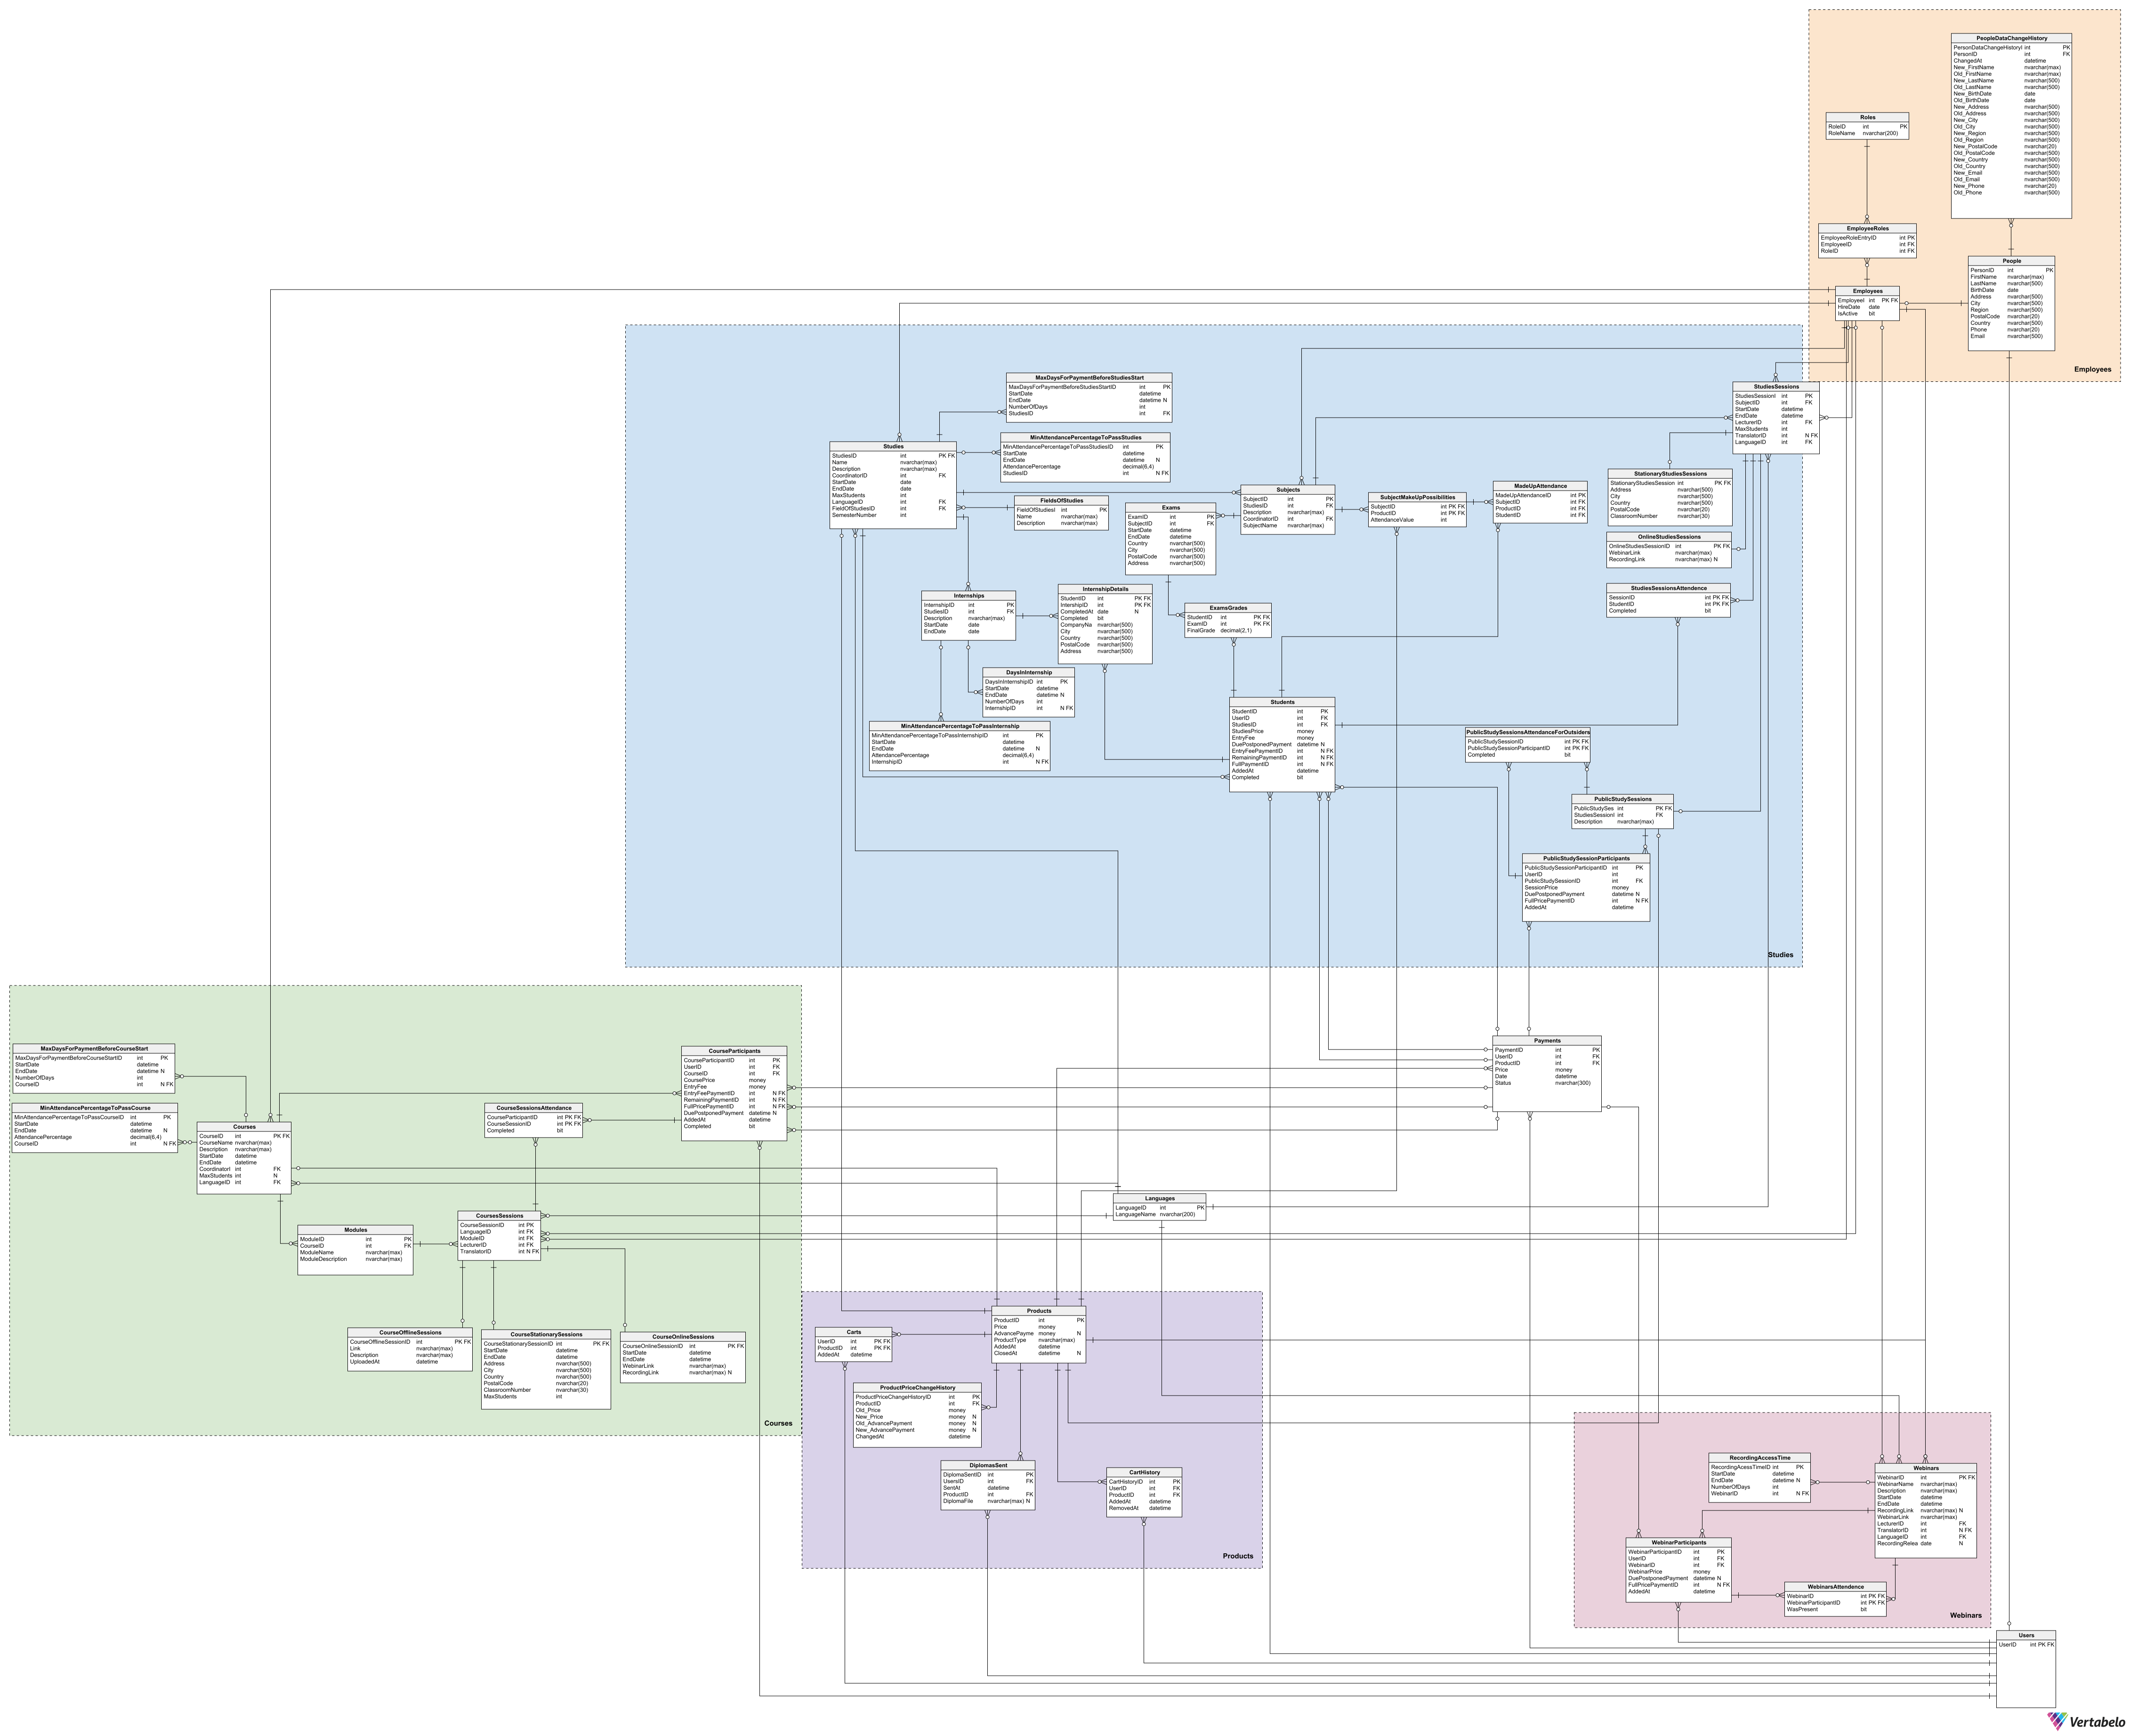
\includegraphics[width=.9\linewidth]{./schemat.png}
\end{center}

\newpage
\begin{center}
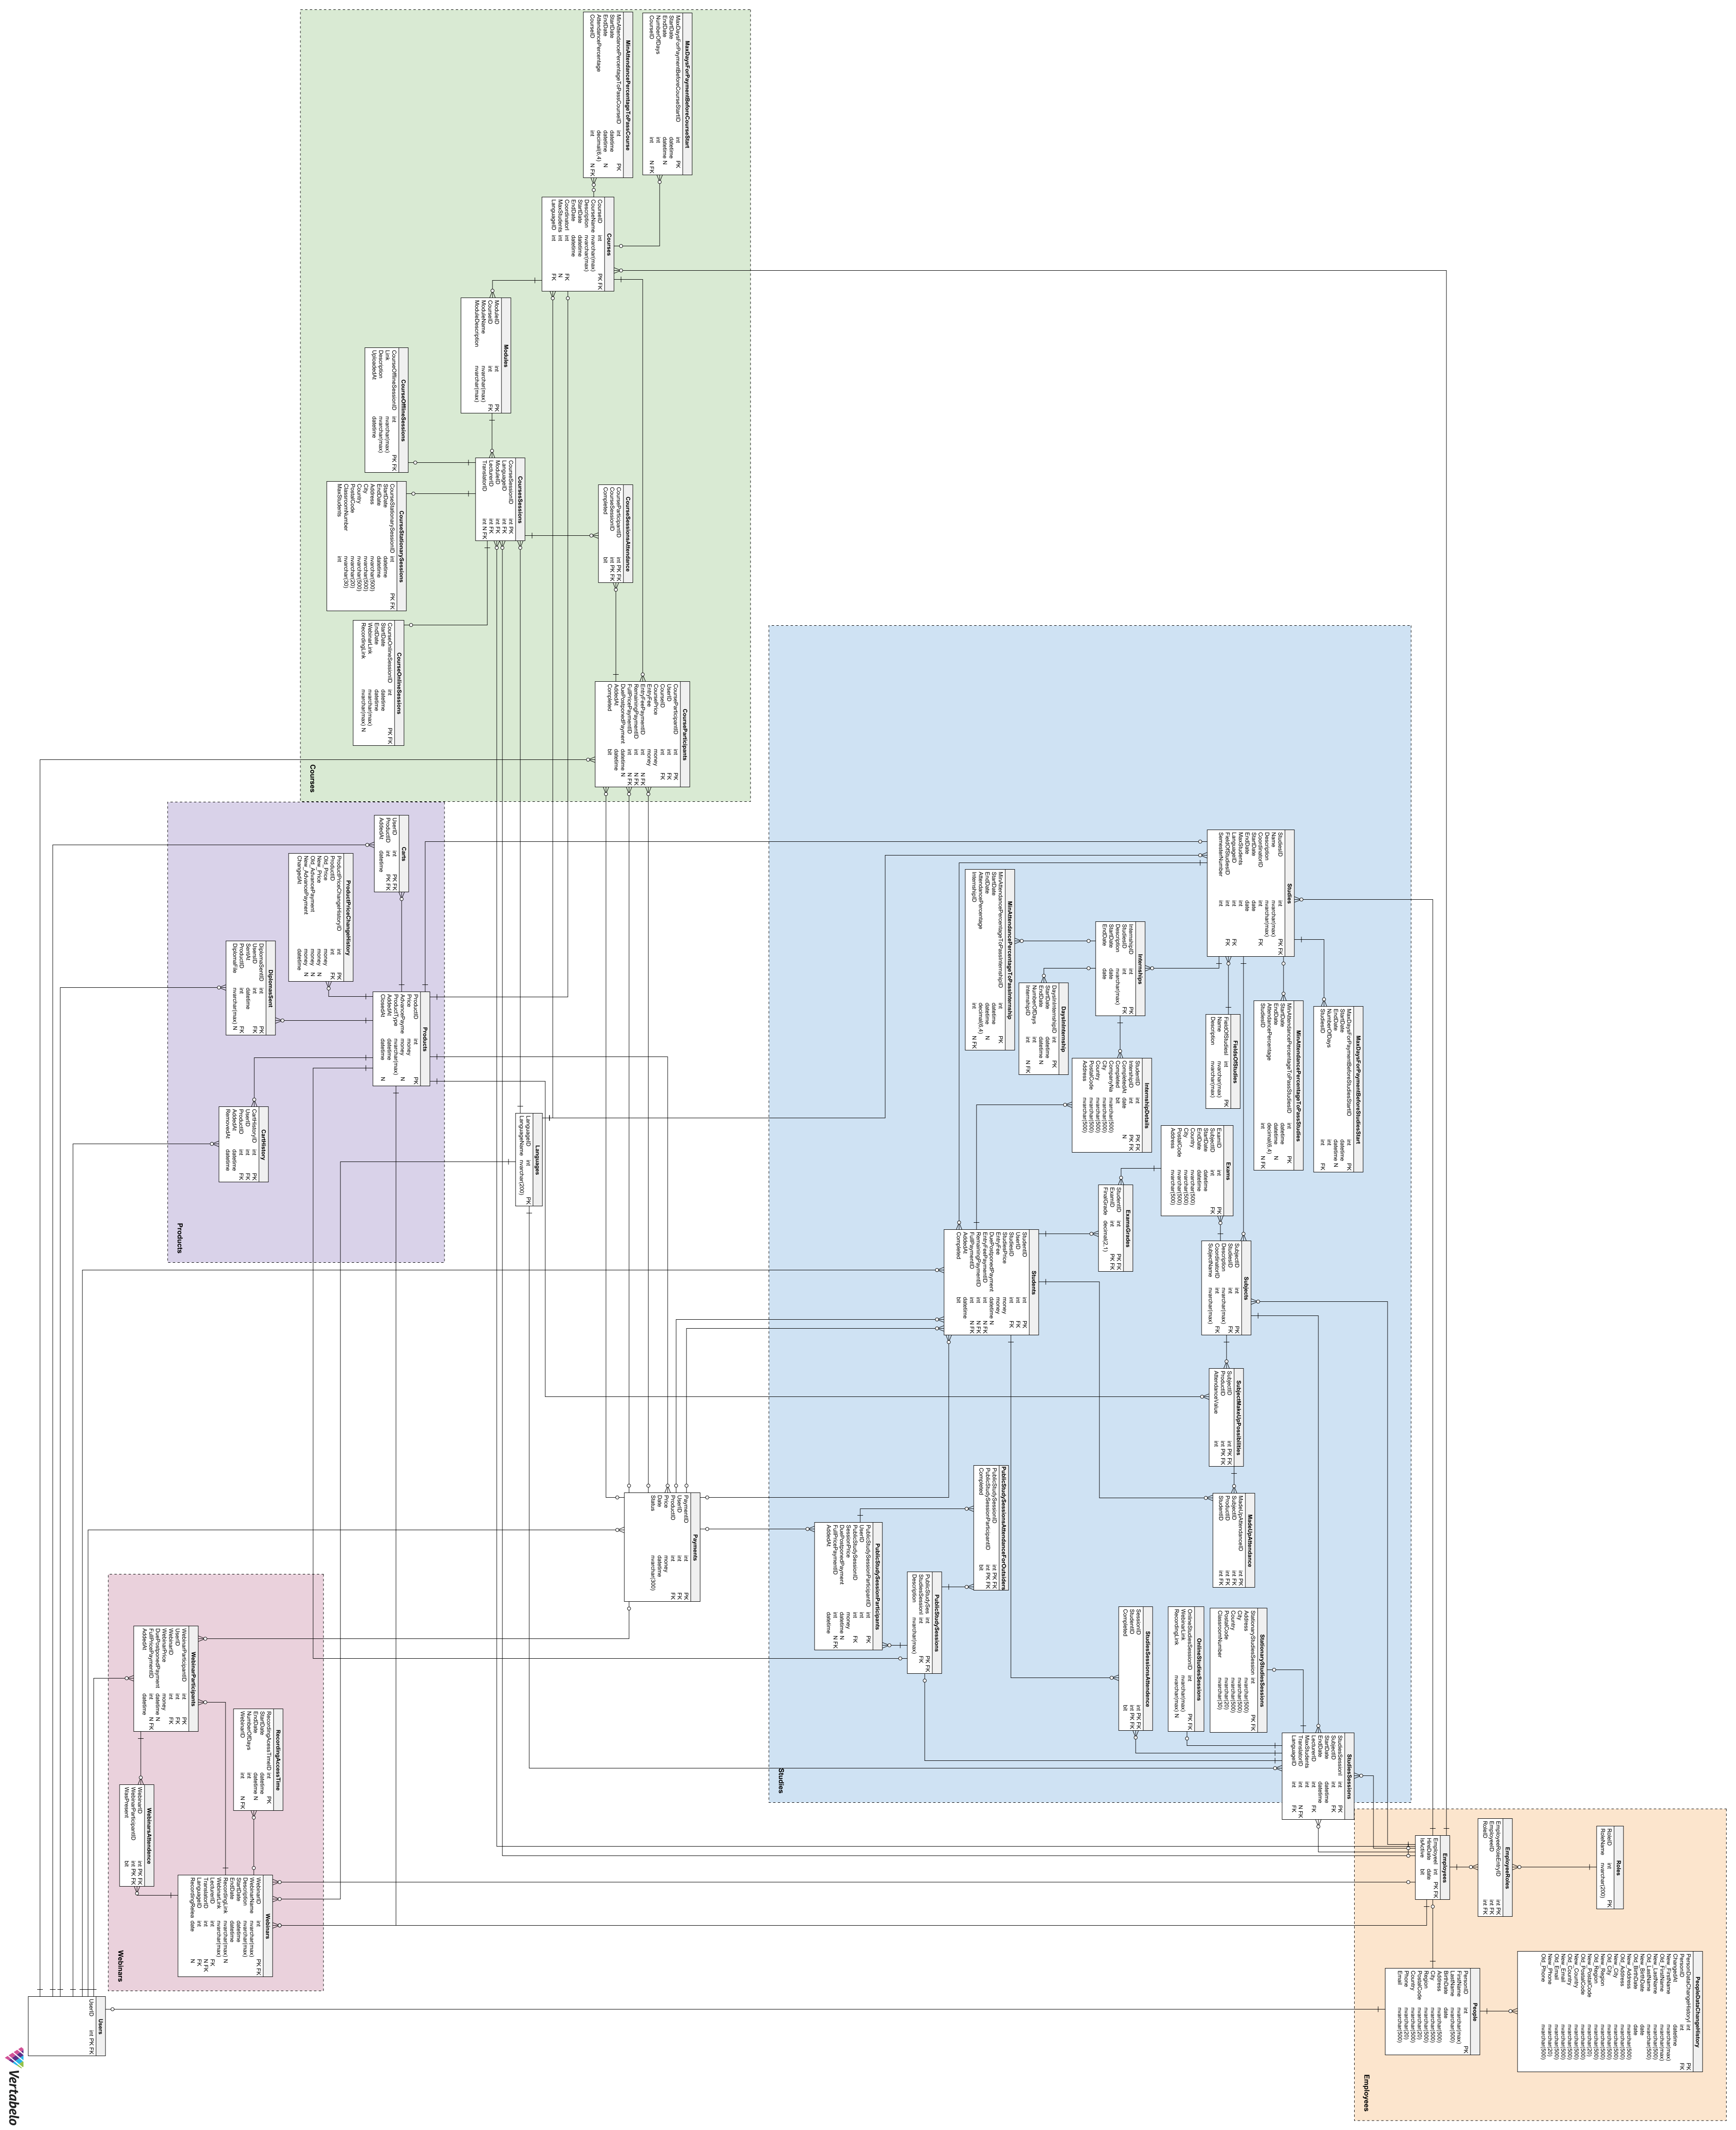
\includegraphics[height=660px]{./schemat-rotated.png}
\end{center}

\newpage
\section{Tabele}
\label{sec:orge22b84c}
\subsection{\texttt{People}}
\label{sec:org2475a43}
Tabela People przechowuje informacje o osobach w systemie.
\begin{itemize}
\item \texttt{PersonID} - Unikalny identyfikator osoby, generowany automatycznie.
\item \texttt{FirstName} - Imię osoby.
\item \texttt{LastName} - Nazwisko osoby.
\item \texttt{BirthDate} - Data urodzenia osoby.
\item \texttt{Address} - Adres zamieszkania osoby.
\item \texttt{City} - Miasto zamieszkania osoby.
\item \texttt{Region} - Region zamieszkania osoby.
\item \texttt{PostalCode} - Kod pocztowy zamieszkania osoby.
\item \texttt{Country} - Kraj zamieszkania osoby.
\item \texttt{Phone} - Numer telefonu osoby.
\item \texttt{Email} - Adres e-mail osoby.
\end{itemize}
\begin{Code}
\begin{Verbatim}
\color{EFD}\EFk{CREATE} \EFk{TABLE} \EFf{People} (
    PersonID \EFt{int}  \EFk{NOT} \EFk{NULL} \EFk{IDENTITY},
    FirstName nvarchar(\EFb{max})  \EFk{NOT} \EFk{NULL},
    LastName nvarchar(\EFhn{500})  \EFk{NOT} \EFk{NULL},
    BirthDate \EFt{date}  \EFk{NOT} \EFk{NULL},
    Address nvarchar(\EFhn{500})  \EFk{NOT} \EFk{NULL},
    City nvarchar(\EFhn{500})  \EFk{NOT} \EFk{NULL},
    Region nvarchar(\EFhn{500})  \EFk{NOT} \EFk{NULL},
    PostalCode nvarchar(\EFhn{20})  \EFk{NOT} \EFk{NULL},
    Country nvarchar(\EFhn{500})  \EFk{NOT} \EFk{NULL},
    Phone nvarchar(\EFhn{20})  \EFk{NOT} \EFk{NULL},
    Email nvarchar(\EFhn{500})  \EFk{NOT} \EFk{NULL},
    \EFk{CONSTRAINT} Person\_pk \EFk{PRIMARY} \EFk{KEY}  (PersonID)
);
\end{Verbatim}
\end{Code}
Warunki integralnościowe:


\begin{itemize}
\item \texttt{People\_EmailValid}

Adres email musi zawierać znak '@'

\begin{Code}
\begin{Verbatim}
\color{EFD}\EFk{CONSTRAINT} People\_EmailValid \EFk{CHECK}
(Email \EFk{LIKE} \EFs{'\%@\%'})
\end{Verbatim}
\end{Code}
\item \texttt{People\_BirthDateValid}

Data urodzenia nie może być z przyszłości
\begin{Code}
\begin{Verbatim}
\color{EFD}\EFk{CONSTRAINT} People\_BirthDateValid \EFk{CHECK}
(BirthDate <= GetDate())
\end{Verbatim}
\end{Code}
\item \texttt{People\_PhoneIsValid}

Numer telefonu składa się z cyfr
\begin{Code}
\begin{Verbatim}
\color{EFD}\EFk{CONSTRAINT} People\_PhoneIsValid \EFk{CHECK}
((ISNUMERIC([Phone])=(\EFhn{1})))
\end{Verbatim}
\end{Code}
\item \texttt{People\_PostalCodeIsValid}

Kod pocztowy musi być w poprawnym formacie.
\begin{Code}
\begin{Verbatim}
\color{EFD}\EFk{CONSTRAINT} People\_PostalCodeIsValid \EFk{CHECK}
(PostalCode \EFk{LIKE} \EFs{'[0-9][0-9]-[0-9][0-9][0-9]'}
\EFk{OR} PostalCode \EFk{LIKE} \EFs{'[0-9][0-9][0-9][0-9][0-9]'}
\EFk{OR} PostalCode \EFk{LIKE} \EFs{'[0-9][0-9][0-9][0-9][0-9][0-9]'})
\end{Verbatim}
\end{Code}
\end{itemize}
\subsection{\texttt{Employees}}
\label{sec:orge77d964}
Tabela Employees przechowuje informacje o pracownikach systemu.
\begin{itemize}
\item \texttt{EmployeeID} - Unikalny identyfikator pracownika, stanowiący klucz główny tabeli.
\item \texttt{HireDate} - Data zatrudnienia pracownika.
\item \texttt{IsActive} - Flaga określająca, czy pracownik jest aktualnie zatrudniony.
\end{itemize}
\begin{Code}
\begin{Verbatim}
\color{EFD}\EFk{CREATE} \EFk{TABLE} \EFf{Employees} (
    EmployeeID \EFt{int}  \EFk{NOT} \EFk{NULL},
    HireDate \EFt{date}  \EFk{NOT} \EFk{NULL},
    IsActive \EFt{bit}  \EFk{NOT} \EFk{NULL},
    \EFk{CONSTRAINT} id \EFk{PRIMARY} \EFk{KEY}  (EmployeeID)
);
\EFk{ALTER} \EFk{TABLE} \EFf{Employees} \EFk{ADD} \EFk{CONSTRAINT} Employees\_People
    \EFk{FOREIGN} \EFk{KEY} (EmployeeID)
    \EFk{REFERENCES} People (PersonID);
\end{Verbatim}
\end{Code}
\subsection{\texttt{Users}}
\label{sec:org00cc62a}
Tabela Users przechowuje podstawowe informacje o użytkownikach.
\begin{itemize}
\item \texttt{UserID} - Unikalny identyfikator użytkownika, stanowiący klucz główny tabeli.
\end{itemize}
\begin{Code}
\begin{Verbatim}
\color{EFD}\EFk{CREATE} \EFk{TABLE} \EFf{Users} (
    UserID \EFt{int}  \EFk{NOT} \EFk{NULL},
    \EFk{CONSTRAINT} Users\_pk \EFk{PRIMARY} \EFk{KEY}  (UserID)
);
\EFk{ALTER} \EFk{TABLE} \EFf{Users} \EFk{ADD} \EFk{CONSTRAINT} Users\_People
    \EFk{FOREIGN} \EFk{KEY} (UserID)
    \EFk{REFERENCES} People (PersonID);
\end{Verbatim}
\end{Code}
\subsection{\texttt{PeopleDataChangeHistory}}
\label{sec:orgd02a234}
Tabela PeopleDataChangeHistory przechowuje historię zmian danych osobowych w systemie.
\begin{itemize}
\item \texttt{PersonDataChangeHistoryID} - Unikalny identyfikator wpisu historii zmian danych osobowych, generowany automatycznie.
\item \texttt{PersonID} - Identyfikator osoby, do której odnosi się historia zmian.
\item \texttt{ChangedAt} - Data i czas dokonania zmiany.
\item \texttt{New\_FirstName} - Nowe imię.
\item \texttt{Old\_FirstName} - Stare imię.
\item \texttt{New\_LastName} - Nowe nazwisko.
\item \texttt{Old\_LastName} - Stare nazwisko.
\item \texttt{New\_BirthDate} - Nowa data urodzenia.
\item \texttt{Old\_BirthDate} - Stara data urodzenia.
\item \texttt{New\_Address} - Nowy adres zamieszkania.
\item \texttt{Old\_Address} - Stary adres zamieszkania.
\item \texttt{New\_City} - Nowe miasto zamieszkania.
\item \texttt{Old\_City} - Stare miasto zamieszkania.
\item \texttt{New\_Region} - Nowy region zamieszkania.
\item \texttt{Old\_Region} - Stary region zamieszkania.
\item \texttt{New\_PostalCode} - Nowy kod pocztowy zamieszkania.
\item \texttt{Old\_PostalCode} - Stary kod pocztowy zamieszkania.
\item \texttt{New\_Country} - Nowy kraj zamieszkania.
\item \texttt{Old\_Country} - Stary kraj zamieszkania.
\item \texttt{New\_Email} - Nowy adres e-mail.
\item \texttt{Old\_Email} - Stary adres e-mail.
\item \texttt{New\_Phone} - Nowy numer telefonu.
\item \texttt{Old\_Phone} - Stary numer telefonu.
\end{itemize}
\begin{Code}
\begin{Verbatim}
\color{EFD}\EFk{CREATE} \EFk{TABLE} \EFf{PeopleDataChangeHistory} (
    PersonDataChangeHistoryID \EFt{int}  \EFk{NOT} \EFk{NULL} \EFk{IDENTITY},
    PersonID \EFt{int}  \EFk{NOT} \EFk{NULL},
    ChangedAt datetime  \EFk{NOT} \EFk{NULL},
    New\_FirstName nvarchar(\EFb{max})  \EFk{NOT} \EFk{NULL},
    Old\_FirstName nvarchar(\EFb{max})  \EFk{NOT} \EFk{NULL},
    New\_LastName nvarchar(\EFhn{500})  \EFk{NOT} \EFk{NULL},
    Old\_LastName nvarchar(\EFhn{500})  \EFk{NOT} \EFk{NULL},
    New\_BirthDate \EFt{date}  \EFk{NOT} \EFk{NULL},
    Old\_BirthDate \EFt{date}  \EFk{NOT} \EFk{NULL},
    New\_Address nvarchar(\EFhn{500})  \EFk{NOT} \EFk{NULL},
    Old\_Address nvarchar(\EFhn{500})  \EFk{NOT} \EFk{NULL},
    New\_City nvarchar(\EFhn{500})  \EFk{NOT} \EFk{NULL},
    Old\_City nvarchar(\EFhn{500})  \EFk{NOT} \EFk{NULL},
    New\_Region nvarchar(\EFhn{500})  \EFk{NOT} \EFk{NULL},
    Old\_Region nvarchar(\EFhn{500})  \EFk{NOT} \EFk{NULL},
    New\_PostalCode nvarchar(\EFhn{20})  \EFk{NOT} \EFk{NULL},
    Old\_PostalCode nvarchar(\EFhn{500})  \EFk{NOT} \EFk{NULL},
    New\_Country nvarchar(\EFhn{500})  \EFk{NOT} \EFk{NULL},
    Old\_Country nvarchar(\EFhn{500})  \EFk{NOT} \EFk{NULL},
    New\_Email nvarchar(\EFhn{500})  \EFk{NOT} \EFk{NULL},
    Old\_Email nvarchar(\EFhn{500})  \EFk{NOT} \EFk{NULL},
    New\_Phone nvarchar(\EFhn{20})  \EFk{NOT} \EFk{NULL},
    Old\_Phone nvarchar(\EFhn{500})  \EFk{NOT} \EFk{NULL},
    \EFk{CONSTRAINT} PersonDataChangeHistory\_pk \EFk{PRIMARY} \EFk{KEY}  (PersonDataChangeHistoryID)
);
\EFk{ALTER} \EFk{TABLE} \EFf{PeopleDataChangeHistory} \EFk{ADD} \EFk{CONSTRAINT} PeopleDataChangeHistory\_People
    \EFk{FOREIGN} \EFk{KEY} (PersonID)
    \EFk{REFERENCES} People (PersonID);
\end{Verbatim}
\end{Code}
Warunki integralnościowe:


\begin{itemize}
\item \texttt{PeopleDataChangeHistory\_ChangedAtIsValid}

Data zmiany nie może być w przyszłości
\begin{Code}
\begin{Verbatim}
\color{EFD}\EFk{CONSTRAINT} PeopleDataChangeHistory\_ChangedAtIsValid \EFk{CHECK}
(ChangedAt <= GetDate())
\end{Verbatim}
\end{Code}
\item \texttt{PeopleDataChangeHistory\_NewPostalCodeIsValid}

Kod pocztowy musi być w poprawnym formacie
\begin{Code}
\begin{Verbatim}
\color{EFD}\EFk{CONSTRAINT} PeopleDataChangeHistory\_NewPostalCodeIsValid \EFk{CHECK}
(New\_PostalCode \EFk{LIKE} \EFs{'[0-9][0-9]-[0-9][0-9][0-9]'}
\EFk{OR} New\_PostalCode \EFk{LIKE} \EFs{'[0-9][0-9][0-9][0-9][0-9]'}
\EFk{OR} New\_PostalCode \EFk{LIKE} \EFs{'[0-9][0-9][0-9][0-9][0-9][0-9]'})
\end{Verbatim}
\end{Code}
\item \texttt{PeopleDataChangeHistory\_New\_EmailValid}

Nowy adres email musi zawierać znak '@'
\begin{Code}
\begin{Verbatim}
\color{EFD}\EFk{CONSTRAINT} PeopleDataChangeHistory\_New\_EmailValid \EFk{CHECK}
(New\_Email \EFk{LIKE} \EFs{'\%@\%'})
\end{Verbatim}
\end{Code}
\item \texttt{PeopleDataChangeHistory\_New\_BirthDate}

Data urodzenia nie może być w przyszłości
\begin{Code}
\begin{Verbatim}
\color{EFD}\EFk{CONSTRAINT} PeopleDataChangeHistory\_New\_BirthDate \EFk{CHECK}
(New\_BirthDate <= GetDate())
\end{Verbatim}
\end{Code}
\item \texttt{PeopleDataChangeHistory\_New\_Phone}

Nowy numer telefonu składa się z cyfr
\begin{Code}
\begin{Verbatim}
\color{EFD}\EFk{CONSTRAINT} PeopleDataChangeHistory\_New\_Phone \EFk{CHECK}
(ISNUMERIC(New\_Phone)=(\EFhn{1}))
\end{Verbatim}
\end{Code}
\end{itemize}
\subsection{\texttt{Roles}}
\label{sec:org0b49b84}
Tabela Roles przechowuje informacje o różnych rolach w systemie.
\begin{itemize}
\item \texttt{RoleID} - Unikalny identyfikator roli, generowany automatycznie.
\item \texttt{RoleName} - Nazwa roli, opisująca jej funkcję lub uprawnienia w systemie.
\end{itemize}
\begin{Code}
\begin{Verbatim}
\color{EFD}\EFk{CREATE} \EFk{TABLE} \EFf{Roles} (
    RoleID \EFt{int}  \EFk{NOT} \EFk{NULL} \EFk{IDENTITY},
    RoleName nvarchar(\EFhn{200})  \EFk{NOT} \EFk{NULL},
    \EFk{CONSTRAINT} RoleName \EFk{UNIQUE} (RoleName),
    \EFk{CONSTRAINT} employeeType \EFk{PRIMARY} \EFk{KEY}  (RoleID)
);
\end{Verbatim}
\end{Code}
\subsection{\texttt{EmployeeRoles}}
\label{sec:org3869524}
Tabela EmployeeRoles przechowuje informacje o rolach przypisanych pracownikom systemu.
\begin{itemize}
\item \texttt{EmployeeRoleEntryID} - Unikalny identyfikator wpisu roli pracownika, który jest generowany automatycznie.
\item \texttt{EmployeeID} - Identyfikator pracownika, do którego przypisana jest rola. Jest to klucz obcy, odnoszący
\end{itemize}
się do kolumny EmployeeID w tabeli Employees.
\begin{itemize}
\item \texttt{RoleID} - Identyfikator roli przypisanej pracownikowi. Jest to klucz obcy, odnoszący się do kolumny RoleID w tabeli Roles.
\end{itemize}

\begin{Code}
\begin{Verbatim}
\color{EFD}\EFk{CREATE} \EFk{TABLE} \EFf{EmployeeRoles} (
    EmployeeRoleEntryID \EFt{int}  \EFk{NOT} \EFk{NULL} \EFk{IDENTITY},
    EmployeeID \EFt{int}  \EFk{NOT} \EFk{NULL},
    RoleID \EFt{int}  \EFk{NOT} \EFk{NULL},
    \EFk{CONSTRAINT} EmployeeRoles\_ak\_1 \EFk{UNIQUE} (EmployeeRoleEntryID, RoleID),
    \EFk{CONSTRAINT} EmployeeRoles\_pk \EFk{PRIMARY} \EFk{KEY}  (EmployeeRoleEntryID)
);
\EFk{ALTER} \EFk{TABLE} \EFf{EmployeeRoles} \EFk{ADD} \EFk{CONSTRAINT} EmployeeCategories\_Employees
    \EFk{FOREIGN} \EFk{KEY} (EmployeeID)
    \EFk{REFERENCES} Employees (EmployeeID)
    \EFk{ON} \EFk{DELETE}  \EFk{CASCADE};
\EFk{ALTER} \EFk{TABLE} \EFf{EmployeeRoles} \EFk{ADD} \EFk{CONSTRAINT} EmployeeRoles\_Roles
    \EFk{FOREIGN} \EFk{KEY} (RoleID)
    \EFk{REFERENCES} Roles (RoleID)
    \EFk{ON} \EFk{DELETE}  \EFk{CASCADE};
\end{Verbatim}
\end{Code}
\subsection{\texttt{Products}}
\label{sec:orgaa3b19e}
Tabela Products przechowuje informacje o produktach w systemie.
\begin{itemize}
\item \texttt{ProductID} - Unikalny identyfikator produktu.
\item \texttt{Price} - Cena produktu.
\item \texttt{AdvancePayment} - Wartość zaliczki do zapłaty za produkt.
\item \texttt{ProductType} - Rodzaj produktu.
\item \texttt{AddedAt} - Data dodania produktu do systemu.
\item \texttt{ClosedAt} - Data zamknięcia produktu, jeżeli produkt nie jest już dostępny.
\end{itemize}
\begin{Code}
\begin{Verbatim}
\color{EFD}\EFk{CREATE} \EFk{TABLE} \EFf{Products} (
    ProductID \EFt{int}  \EFk{NOT} \EFk{NULL} \EFk{IDENTITY},
    Price money  \EFk{NOT} \EFk{NULL},
    AdvancePayment money  \EFk{NULL},
    ProductType nvarchar(\EFb{max})  \EFk{NOT} \EFk{NULL},
    AddedAt datetime  \EFk{NOT} \EFk{NULL} \EFk{DEFAULT} GETDATE(),
    ClosedAt datetime  \EFk{NULL},
    \EFk{CONSTRAINT} Products\_pk \EFk{PRIMARY} \EFk{KEY}  (ProductID)
);
\end{Verbatim}
\end{Code}
Warunki integralnościowe:


\begin{itemize}
\item \texttt{Products\_PriceIsValid}

Cena musi być większa lub równa 0
\begin{Code}
\begin{Verbatim}
\color{EFD}\EFk{CONSTRAINT} Products\_PriceIsValid \EFk{CHECK}
(Price >= \EFhn{0})
\end{Verbatim}
\end{Code}
\item \texttt{Products\_AdvancePaymentIsValid}

Zaliczka musi być większa od 0 i nie może być większa od ceny całkowitej, lub być NULL
\begin{Code}
\begin{Verbatim}
\color{EFD}\EFk{CONSTRAINT} Products\_AdvancePaymentIsValid \EFk{CHECK}
((AdvancePayment > \EFhn{0} \EFk{AND} AdvancePayment < Price)
\EFk{OR} (AdvancePayment \EFk{IS} \EFk{NULL}))
\end{Verbatim}
\end{Code}
\item \texttt{Products\_ProductTypeIsValid}

Produkt może być webinarem, kursem, studia mi, albo pojedyńczym postkaniem studyjnym
\begin{Code}
\begin{Verbatim}
\color{EFD}\EFk{CONSTRAINT} Products\_ProductTypeIsValid \EFk{CHECK}
(ProductType \EFk{IN} (\EFs{'studies'}, \EFs{'course'},\EFs{'webinar'}, \EFs{'public study session'}))
\end{Verbatim}
\end{Code}
\item \texttt{Products\_AddedAtIsValid}

AddedAt nie może być w przyszłości
\begin{Code}
\begin{Verbatim}
\color{EFD}\EFk{CONSTRAINT} Products\_AddedAtIsValid \EFk{CHECK}
(AddedAt <= GetDate())
\end{Verbatim}
\end{Code}
\item \texttt{Products\_ClosedAtIsValid}

ClosedAt musi być po AddedAt
\begin{Code}
\begin{Verbatim}
\color{EFD}\EFk{CONSTRAINT} Products\_ClosedAtIsValid \EFk{CHECK}
(ClosedAt <= GetDate() \EFk{AND} ClosedAt >= AddedAt)
\end{Verbatim}
\end{Code}
\end{itemize}
\subsection{\texttt{ProductPriceChangeHistory}}
\label{sec:org6b35b59}
Tabela ProductPriceChangeHistory przechowuje historię zmian cen produktów.
\begin{itemize}
\item \texttt{ProductPriceChangeHistoryID} - Unikalny identyfikator historii zmian cen produktów.
\item \texttt{ProductID} - Identyfikator produktu, którego cena uległa zmianie.
\item \texttt{Old\_Price} - Stara cena produktu przed zmianą.
\item \texttt{New\_Price} - Nowa cena produktu po zmianie.
\item \texttt{Old\_AdvancePayment} - Stara wartość zaliczki przed zmianą.
\item \texttt{New\_AdvancePayment} - Nowa wartość zaliczki po zmianie.
\item \texttt{ChangedAt} - Data dokonania zmiany.
\end{itemize}
\begin{Code}
\begin{Verbatim}
\color{EFD}\EFk{CREATE} \EFk{TABLE} \EFf{ProductPriceChangeHistory} (
    ProductPriceChangeHistoryID \EFt{int}  \EFk{NOT} \EFk{NULL} \EFk{IDENTITY},
    ProductID \EFt{int}  \EFk{NOT} \EFk{NULL},
    Old\_Price money  \EFk{NOT} \EFk{NULL},
    New\_Price money  \EFk{NULL},
    Old\_AdvancePayment money  \EFk{NULL},
    New\_AdvancePayment money  \EFk{NULL},
    ChangedAt datetime  \EFk{NOT} \EFk{NULL} \EFk{DEFAULT} GETDATE(),
    \EFk{CONSTRAINT} ProductPriceChangeHistory\_pk \EFk{PRIMARY} \EFk{KEY}  (ProductPriceChangeHistoryID)
);
\EFk{ALTER} \EFk{TABLE} \EFf{ProductPriceChangeHistory} \EFk{ADD} \EFk{CONSTRAINT} ProductHistory\_Products
    \EFk{FOREIGN} \EFk{KEY} (ProductID)
    \EFk{REFERENCES} Products (ProductID)
    \EFk{ON} \EFk{DELETE}  \EFk{CASCADE};
\end{Verbatim}
\end{Code}
Warunki integralnościowe:


\begin{itemize}
\item \texttt{ProductHistory\_ChangedAtIsValid}

ChangedAt nie może być z przyszłości
\begin{Code}
\begin{Verbatim}
\color{EFD}\EFk{CONSTRAINT} ProductHistory\_ChangedAtIsValid \EFk{CHECK}
(ChangedAt <= GetDate())
\end{Verbatim}
\end{Code}
\item \texttt{ProductHIstory\_NewPriceIsValid}

Nowa cenu musi być nieujemna
\begin{Code}
\begin{Verbatim}
\color{EFD}\EFk{CONSTRAINT} ProductHIstory\_NewPriceIsValid \EFk{CHECK}
(New\_price >= \EFhn{0})
\end{Verbatim}
\end{Code}
\item \texttt{ProductHistory\_NewAdvancePaymentIsValid}

Jeżeli wpisano zaliczkę to musi być ona większa od zera
\begin{Code}
\begin{Verbatim}
\color{EFD}\EFk{CONSTRAINT} ProductHistory\_NewAdvancePaymentIsValid \EFk{CHECK}
(New\_AdvancePayment > \EFhn{0})
\end{Verbatim}
\end{Code}
\end{itemize}
\subsection{\texttt{Payments}}
\label{sec:org32092b7}
Tabela Payments przechowuje informacje o płatnościach dokonanych przez użytkowników.
\begin{itemize}
\item \texttt{PaymentID} - Unikalny identyfikator płatności.
\item \texttt{UserID} - Identyfikator użytkownika, który dokonał płatności.
\item \texttt{ProductID} - Identyfikator produktu, na który użytkownik dokonał płatności.
\item \texttt{Price} - Kwota płatności.
\item \texttt{Date} - Data dokonania płatności.
\item \texttt{Status} - Status płatności ``Successful'' albo ``Failed''
\end{itemize}
\begin{Code}
\begin{Verbatim}
\color{EFD}\EFk{CREATE} \EFk{TABLE} \EFf{Payments} (
    PaymentID \EFt{int}  \EFk{NOT} \EFk{NULL} \EFk{IDENTITY},
    UserID \EFt{int}  \EFk{NOT} \EFk{NULL},
    ProductID \EFt{int}  \EFk{NOT} \EFk{NULL},
    Price money  \EFk{NOT} \EFk{NULL},
    \EFt{Date} datetime  \EFk{NOT} \EFk{NULL},
    Status nvarchar(\EFhn{300})  \EFk{NOT} \EFk{NULL},
    \EFk{CONSTRAINT} Payments\_pk \EFk{PRIMARY} \EFk{KEY}  (PaymentID)
);
\EFk{ALTER} \EFk{TABLE} \EFf{Payments} \EFk{ADD} \EFk{CONSTRAINT} OrderHistory\_Products
    \EFk{FOREIGN} \EFk{KEY} (ProductID)
    \EFk{REFERENCES} Products (ProductID);
\EFk{ALTER} \EFk{TABLE} \EFf{Payments} \EFk{ADD} \EFk{CONSTRAINT} OrderHistory\_Users
    \EFk{FOREIGN} \EFk{KEY} (UserID)
    \EFk{REFERENCES} Users (UserID);
\end{Verbatim}
\end{Code}
Warunki integralnościowe:


\begin{itemize}
\item \texttt{Payments\_Price}

Kwota musi być  >= 0
\begin{Code}
\begin{Verbatim}
\color{EFD}\EFk{CONSTRAINT} Payments\_Price \EFk{CHECK}
(Price >= \EFhn{0})
\end{Verbatim}
\end{Code}
\item \texttt{Payments\_Status}

Możliwe wartości dla statusu płatności: ``Successful'', ``Failed''
\begin{Code}
\begin{Verbatim}
\color{EFD}\EFk{CONSTRAINT} Payments\_Status \EFk{CHECK}
(Status \EFk{in} (\EFs{'Successful'}, \EFs{'Failed'}))
\end{Verbatim}
\end{Code}
\item \texttt{Payments\_Date}

Data płatności nie może być z przyszłości
\begin{Code}
\begin{Verbatim}
\color{EFD}\EFk{CONSTRAINT} Payments\_Date \EFk{CHECK}
(\EFt{Date} <= GetDate())
\end{Verbatim}
\end{Code}
\end{itemize}
\subsection{\texttt{Carts}}
\label{sec:org430c4bb}
Tabela Carts przechowuje informacje o koszykach zakupowych użytkowników.
\begin{itemize}
\item \texttt{UserID} - Identyfikator użytkownika, do którego przypisany jest koszyk.
\item \texttt{ProductID} - Identyfikator produktu, który został dodany do koszyka.
\item \texttt{AddedAt} - Data i godzina dodania produktu do koszyka. Wartość domyślna to bieżąca data i czas.
\end{itemize}
\begin{Code}
\begin{Verbatim}
\color{EFD}\EFk{CREATE} \EFk{TABLE} \EFf{Carts} (
    UserID \EFt{int}  \EFk{NOT} \EFk{NULL},
    ProductID \EFt{int}  \EFk{NOT} \EFk{NULL},
    AddedAt datetime  \EFk{NOT} \EFk{NULL} \EFk{DEFAULT} GEtDATE(),
    \EFk{CONSTRAINT} Carts\_pk \EFk{PRIMARY} \EFk{KEY}  (UserID,ProductID)
);
\EFk{ALTER} \EFk{TABLE} \EFf{Carts} \EFk{ADD} \EFk{CONSTRAINT} Carts\_Products
    \EFk{FOREIGN} \EFk{KEY} (ProductID)
    \EFk{REFERENCES} Products (ProductID);
\EFk{ALTER} \EFk{TABLE} \EFf{Carts} \EFk{ADD} \EFk{CONSTRAINT} Carts\_Users
    \EFk{FOREIGN} \EFk{KEY} (UserID)
    \EFk{REFERENCES} Users (UserID);
\end{Verbatim}
\end{Code}
Warunki integralnościowe:


\begin{itemize}
\item \texttt{Carts\_AddedAtIsValid}

AddedAt nie może być w przyszłości
\begin{Code}
\begin{Verbatim}
\color{EFD}\EFk{CONSTRAINT} Carts\_AddedAtIsValid \EFk{CHECK}
(AddedAt <= GetDate())
\end{Verbatim}
\end{Code}
\end{itemize}
\subsection{\texttt{CartHistory}}
\label{sec:orgedaae55}
Tabela CartHistory przechowuje historię zmian w koszyku zakupowym.
\begin{itemize}
\item \texttt{CartHistoryID} - Unikalny identyfikator historii koszyka.
\item \texttt{UserID} - Identyfikator użytkownika, do którego przypisana jest historia koszyka.
\item \texttt{ProductID} - Identyfikator produktu, który był dodany do koszyka.
\item \texttt{AddedAt} - Data dodania produktu do koszyka.
\item \texttt{RemovedAt} - Data usunięcia produktu z koszyka.
\end{itemize}
\begin{Code}
\begin{Verbatim}
\color{EFD}\EFk{CREATE} \EFk{TABLE} \EFf{CartHistory} (
    CartHistoryID \EFt{int}  \EFk{NOT} \EFk{NULL} \EFk{IDENTITY},
    UserID \EFt{int}  \EFk{NOT} \EFk{NULL},
    ProductID \EFt{int}  \EFk{NOT} \EFk{NULL},
    AddedAt datetime  \EFk{NOT} \EFk{NULL},
    RemovedAt datetime  \EFk{NOT} \EFk{NULL},
    \EFk{CONSTRAINT} CartHistory\_pk \EFk{PRIMARY} \EFk{KEY}  (CartHistoryID)
);
\EFk{ALTER} \EFk{TABLE} \EFf{CartHistory} \EFk{ADD} \EFk{CONSTRAINT} CartHistory\_Products
    \EFk{FOREIGN} \EFk{KEY} (ProductID)
    \EFk{REFERENCES} Products (ProductID);
\EFk{ALTER} \EFk{TABLE} \EFf{CartHistory} \EFk{ADD} \EFk{CONSTRAINT} CartHistory\_Users
    \EFk{FOREIGN} \EFk{KEY} (UserID)
    \EFk{REFERENCES} Users (UserID);
\end{Verbatim}
\end{Code}
Warunki integralnościowe:


\begin{itemize}
\item \texttt{CartHistory\_AddedAt}

AddedAt nie może być w przyszłości
\begin{Code}
\begin{Verbatim}
\color{EFD}\EFk{CONSTRAINT} CartHistory\_AddedAt \EFk{CHECK}
(AddedAt <= GetDate())
\end{Verbatim}
\end{Code}
\item \texttt{CartHIstory\_RemovedAt}

RemovedAt musi być po AddedAt
\begin{Code}
\begin{Verbatim}
\color{EFD}\EFk{CONSTRAINT} CartHIstory\_RemovedAt \EFk{CHECK}
(RemovedAt >= AddedAt \EFk{AND} RemovedAt <= GetDate())
\end{Verbatim}
\end{Code}
\end{itemize}
\subsection{\texttt{Languages}}
\label{sec:org45e2f5f}
Tabela Languages przechowuje informacje o dostępnych językach w systemie.
\begin{itemize}
\item \texttt{LanguageID} - Unikalny identyfikator języka, generowany automatycznie.
\item \texttt{LanguageName} - Nazwa języka, opisująca konkretny język używany w systemie.
\end{itemize}
\begin{Code}
\begin{Verbatim}
\color{EFD}\EFk{CREATE} \EFk{TABLE} \EFf{Languages} (
    LanguageID \EFt{int}  \EFk{NOT} \EFk{NULL} \EFk{IDENTITY},
    LanguageName nvarchar(\EFhn{200})  \EFk{NOT} \EFk{NULL},
    \EFk{CONSTRAINT} LanguageName \EFk{UNIQUE} (LanguageName),
    \EFk{CONSTRAINT} Languages\_pk \EFk{PRIMARY} \EFk{KEY}  (LanguageID)
);
\end{Verbatim}
\end{Code}
\subsection{\texttt{Webinars}}
\label{sec:org3b0c4a2}
Tabela Webinars przechowuje informacje dotyczące webinarów oferowanych w systemie.
\begin{itemize}
\item \texttt{WebinarID} - Unikalny identyfikator webinaru.
\item \texttt{WebinarName} - Nazwa webinaru.
\item \texttt{Description} - Opis webinaru, zawierający informacje na temat treści i celów.
\item \texttt{StartDate} - Data rozpoczęcia webinaru.
\item \texttt{EndDate} - Data zakończenia webinaru.
\item \texttt{RecordingLink} - Link do nagrania webinaru (opcjonalny).
\item \texttt{WebinarLink} - Link do udziału w webinarze.
\item \texttt{LecturerID} - Identyfikator prowadzącego webinar, który jest pracownikiem systemu.
\item \texttt{TranslatorID} - Identyfikator tłumacza webinaru (opcjonalny).
\item \texttt{LanguageID} - Identyfikator języka, w jakim prowadzony jest webinar.
\item \texttt{RecordingReleaseDate} - Data udostępnienia nagrania webinaru (opcjonalna).
\end{itemize}
\begin{Code}
\begin{Verbatim}
\color{EFD}\EFk{CREATE} \EFk{TABLE} \EFf{Webinars} (
    WebinarID \EFt{int}  \EFk{NOT} \EFk{NULL},
    WebinarName nvarchar(\EFb{max})  \EFk{NOT} \EFk{NULL},
    Description nvarchar(\EFb{max})  \EFk{NOT} \EFk{NULL},
    StartDate datetime  \EFk{NOT} \EFk{NULL},
    EndDate datetime  \EFk{NOT} \EFk{NULL},
    RecordingLink nvarchar(\EFb{max})  \EFk{NULL},
    WebinarLink nvarchar(\EFb{max})  \EFk{NOT} \EFk{NULL},
    LecturerID \EFt{int}  \EFk{NOT} \EFk{NULL},
    TranslatorID \EFt{int}  \EFk{NULL},
    LanguageID \EFt{int}  \EFk{NOT} \EFk{NULL},
    RecordingReleaseDate \EFt{date}  \EFk{NULL},
    \EFk{CONSTRAINT} Webinars\_pk \EFk{PRIMARY} \EFk{KEY}  (WebinarID)
);
\EFk{ALTER} \EFk{TABLE} \EFf{Webinars} \EFk{ADD} \EFk{CONSTRAINT} Webinars\_Languages
    \EFk{FOREIGN} \EFk{KEY} (LanguageID)
    \EFk{REFERENCES} Languages (LanguageID);
\EFk{ALTER} \EFk{TABLE} \EFf{Webinars} \EFk{ADD} \EFk{CONSTRAINT} Webinars\_Lecturers
    \EFk{FOREIGN} \EFk{KEY} (TranslatorID)
    \EFk{REFERENCES} Employees (EmployeeID);
\EFk{ALTER} \EFk{TABLE} \EFf{Webinars} \EFk{ADD} \EFk{CONSTRAINT} Webinars\_Products
    \EFk{FOREIGN} \EFk{KEY} (WebinarID)
    \EFk{REFERENCES} Products (ProductID);
\EFk{ALTER} \EFk{TABLE} \EFf{Webinars} \EFk{ADD} \EFk{CONSTRAINT} Webinars\_Translators
    \EFk{FOREIGN} \EFk{KEY} (LecturerID)
    \EFk{REFERENCES} Employees (EmployeeID);
\end{Verbatim}
\end{Code}
Warunki integralnościowe:


\begin{itemize}
\item \texttt{Webinars\_RecodingReleaseDateValid}

RecodingReleaseData musi być po EndDate
\begin{Code}
\begin{Verbatim}
\color{EFD}\EFk{CONSTRAINT} Webinars\_RecodingReleaseDateValid \EFk{CHECK}
(RecordingReleaseDate >= EndDate)
\end{Verbatim}
\end{Code}
\item \texttt{Webinars\_RecodingLinkRelationWithRecordingReleaseDate}

Jeżeli jest nagranie to RecordingReleaseDate nie może być nullem, jeżeli nie ma to RecordingReleaseDate musi być nullem
\begin{Code}
\begin{Verbatim}
\color{EFD}\EFk{CONSTRAINT} Webinars\_RecodingLinkRelationWithRecordingReleaseDate \EFk{CHECK}
((RecordingReleaseDate \EFk{IS} \EFk{NULL} \EFk{AND} RecordingLink \EFk{IS} \EFk{NULL})
\EFk{OR}
(RecordingReleaseDate \EFk{IS} \EFk{NOT} \EFk{NULL} \EFk{AND} RecordingLink \EFk{IS} \EFk{NOT} \EFk{NULL}))
\end{Verbatim}
\end{Code}
\item \texttt{Webinars\_DateRangeIsValid}

StartDate musi być przed EndDate
\begin{Code}
\begin{Verbatim}
\color{EFD}\EFk{CONSTRAINT} Webinars\_DateRangeIsValid \EFk{CHECK}
(StartDate < EndDate)
\end{Verbatim}
\end{Code}
\end{itemize}
\subsection{\texttt{WebinarParticipants}}
\label{sec:org44cd8b7}
Tabela WebinarParticipants przechowuje informacje o uczestnikach webinarów.
\begin{itemize}
\item \texttt{WebinarParticipantID} - Unikalny identyfikator uczestnika webinaru.
\item \texttt{UserID} - Identyfikator użytkownika, który jest uczestnikiem webinaru.
\item \texttt{WebinarID} - Identyfikator webinaru, do którego przypisany jest uczestnik.
\item \texttt{WebinarPrice} - Cena uczestnictwa w webinarze.
\item \texttt{DuePostponedPayment} - Data odroczonego terminu płatności.
\item \texttt{FullPricePaymentID} - Identyfikator pełnej płatności.
\item \texttt{AddedAt} - Data dodania uczestnika do webinaru.
\end{itemize}
\begin{Code}
\begin{Verbatim}
\color{EFD}\EFk{CREATE} \EFk{TABLE} \EFf{WebinarParticipants} (
    WebinarParticipantID \EFt{int}  \EFk{NOT} \EFk{NULL} \EFk{IDENTITY},
    UserID \EFt{int}  \EFk{NOT} \EFk{NULL},
    WebinarID \EFt{int}  \EFk{NOT} \EFk{NULL},
    WebinarPrice money  \EFk{NOT} \EFk{NULL},
    DuePostponedPayment datetime  \EFk{NULL},
    FullPricePaymentID \EFt{int}  \EFk{NULL},
    AddedAt datetime  \EFk{NOT} \EFk{NULL} \EFk{DEFAULT} GETDATE(),
    \EFk{CONSTRAINT} WebinarParticipants\_pk \EFk{PRIMARY} \EFk{KEY}  (WebinarParticipantID)
);
\EFk{ALTER} \EFk{TABLE} \EFf{WebinarParticipants} \EFk{ADD} \EFk{CONSTRAINT} WebinarParticipants\_Payments
    \EFk{FOREIGN} \EFk{KEY} (FullPricePaymentID)
    \EFk{REFERENCES} Payments (PaymentID)
    \EFk{ON} \EFk{DELETE}  \EFk{CASCADE};
\EFk{ALTER} \EFk{TABLE} \EFf{WebinarParticipants} \EFk{ADD} \EFk{CONSTRAINT} WebinarParticipants\_Users
    \EFk{FOREIGN} \EFk{KEY} (UserID)
    \EFk{REFERENCES} Users (UserID)
    \EFk{ON} \EFk{DELETE}  \EFk{CASCADE};
\EFk{ALTER} \EFk{TABLE} \EFf{WebinarParticipants} \EFk{ADD} \EFk{CONSTRAINT} WebinarParticipants\_Webinars
    \EFk{FOREIGN} \EFk{KEY} (WebinarID)
    \EFk{REFERENCES} Webinars (WebinarID)
    \EFk{ON} \EFk{DELETE}  \EFk{CASCADE};
\end{Verbatim}
\end{Code}
Warunki integralnościowe:


\begin{itemize}
\item \texttt{WebinarParticipants\_WebinarPrice}

Cena za webinar musi być większa lub równa zero
\begin{Code}
\begin{Verbatim}
\color{EFD}\EFk{CONSTRAINT} WebinarParticipants\_WebinarPrice \EFk{CHECK}
(WebinarPrice >= \EFhn{0})
\end{Verbatim}
\end{Code}
\item \texttt{WebinarParticipants\_FulPricePaymentID}

FullPricePaymentID może być NULL gdy istnieje DuePostponedPayment lub gdy WebinarPrice = 0
\begin{Code}
\begin{Verbatim}
\color{EFD}\EFk{CONSTRAINT} WebinarParticipants\_FulPricePaymentID \EFk{CHECK}
(FullPricePaymentID \EFk{IS} \EFk{NOT} \EFk{NULL} \EFk{OR}
 (DuePostponedPayment \EFk{IS} \EFk{NOT} \EFk{NULL} \EFk{OR}
     WebinarPrice = \EFhn{0}))
\end{Verbatim}
\end{Code}
\end{itemize}
\subsection{\texttt{WebinarsAttendence}}
\label{sec:org8c6867f}
Tabela WebinarsAttendance przechowuje informacje dotyczące uczestnictwa w webinarze.
\begin{itemize}
\item \texttt{WebinarID} - Identyfikator webinaru, do którego odnosi się uczestnictwo.
\item \texttt{WebinarParticipantID} - Identyfikator uczestnika webinaru.
\item \texttt{WasPresent} - Wartość logiczna określająca, czy uczestnik był obecny na webinarze (1 - obecny, 0 - nieobecny).
\end{itemize}
\begin{Code}
\begin{Verbatim}
\color{EFD}\EFk{CREATE} \EFk{TABLE} \EFf{WebinarsAttendence} (
    WebinarID \EFt{int}  \EFk{NOT} \EFk{NULL},
    WebinarParticipantID \EFt{int}  \EFk{NOT} \EFk{NULL},
    WasPresent \EFt{bit}  \EFk{NOT} \EFk{NULL},
    \EFk{CONSTRAINT} WebinarsAttendence\_pk \EFk{PRIMARY} \EFk{KEY}  (WebinarID,WebinarParticipantID)
);
\EFk{ALTER} \EFk{TABLE} \EFf{WebinarsAttendence} \EFk{ADD} \EFk{CONSTRAINT} WebinarsAttendence\_WebinarParticipants
    \EFk{FOREIGN} \EFk{KEY} (WebinarParticipantID)
    \EFk{REFERENCES} WebinarParticipants (WebinarParticipantID);
\EFk{ALTER} \EFk{TABLE} \EFf{WebinarsAttendence} \EFk{ADD} \EFk{CONSTRAINT} WebinarsAttendence\_Webinars
    \EFk{FOREIGN} \EFk{KEY} (WebinarID)
    \EFk{REFERENCES} Webinars (WebinarID)
    \EFk{ON} \EFk{DELETE}  \EFk{CASCADE};
\end{Verbatim}
\end{Code}
\subsection{\texttt{Courses}}
\label{sec:orgaa2e6e4}
Tabela Courses przechowuje informacje o kursach dostępnych w systemie.
\begin{itemize}
\item \texttt{CourseID} - Unikalny identyfikator kursu.
\item \texttt{CourseName} - Nazwa kursu.
\item \texttt{Description} - Opis kursu, zawierający informacje dotyczące treści i celów.
\item \texttt{StartDate} - Data rozpoczęcia kursu.
\item \texttt{EndDate} - Data zakończenia kursu.

\item \texttt{CoordinatorID} - Identyfikator koordynatora kursu, który jest pracownikiem systemu.
\item \texttt{MaxStudents} - Maksymalna liczba studentów, którzy mogą uczestniczyć w kursie.
\item \texttt{LanguageID} - Identyfikator języka, w jakim prowadzony jest kurs.
\end{itemize}
\begin{Code}
\begin{Verbatim}
\color{EFD}\EFk{CREATE} \EFk{TABLE} \EFf{Courses} (
    CourseID \EFt{int}  \EFk{NOT} \EFk{NULL},
    CourseName nvarchar(\EFb{max})  \EFk{NOT} \EFk{NULL},
    Description nvarchar(\EFb{max})  \EFk{NOT} \EFk{NULL},
    StartDate datetime  \EFk{NOT} \EFk{NULL},
    EndDate datetime  \EFk{NOT} \EFk{NULL},
    CoordinatorID \EFt{int}  \EFk{NOT} \EFk{NULL},
    MaxStudents \EFt{int}  \EFk{NULL},
    LanguageID \EFt{int}  \EFk{NOT} \EFk{NULL},
    \EFk{CONSTRAINT} Courses\_pk \EFk{PRIMARY} \EFk{KEY}  (CourseID)
);
\EFk{ALTER} \EFk{TABLE} \EFf{Courses} \EFk{ADD} \EFk{CONSTRAINT} Courses\_Employees
    \EFk{FOREIGN} \EFk{KEY} (CoordinatorID)
    \EFk{REFERENCES} Employees (EmployeeID);
\EFk{ALTER} \EFk{TABLE} \EFf{Courses} \EFk{ADD} \EFk{CONSTRAINT} Courses\_Languages
    \EFk{FOREIGN} \EFk{KEY} (LanguageID)
    \EFk{REFERENCES} Languages (LanguageID);
\EFk{ALTER} \EFk{TABLE} \EFf{Courses} \EFk{ADD} \EFk{CONSTRAINT} Courses\_Products
    \EFk{FOREIGN} \EFk{KEY} (CourseID)
    \EFk{REFERENCES} Products (ProductID);
\end{Verbatim}
\end{Code}
Warunki integralnościowe:


\begin{itemize}
\item \texttt{Course\_MaxStudents}

MaxStudents może być NULL, jeżeli np. jest to kurs wyłącznie online, w przeciwnym wypadku musi być > 0
\begin{Code}
\begin{Verbatim}
\color{EFD}\EFk{CONSTRAINT} Course\_MaxStudents \EFk{CHECK}
(MaxStudents \EFk{is} \EFk{NULL} \EFk{OR}
(MaxStudents > \EFhn{0}) )
\end{Verbatim}
\end{Code}
\item \texttt{Course\_DateIntervalIsValid}

EndDate musi być po StartDate
\begin{Code}
\begin{Verbatim}
\color{EFD}\EFk{CONSTRAINT} Course\_DateIntervalIsValid \EFk{CHECK}
(StartDate < EndDate)
\end{Verbatim}
\end{Code}
\end{itemize}
\subsection{\texttt{CourseParticipants}}
\label{sec:orga4da90c}
Tabela CourseParticipants przechowuje informacje o uczestnikach kursów.
\begin{itemize}
\item \texttt{CourseParticipantID} - Unikalny identyfikator uczestnika kursu.
\item \texttt{UserID} - Identyfikator użytkownika, który jest jednocześnie kluczem obcym powiązanym z tabelą Users.
\item \texttt{CourseID} - Identyfikator kursu, który jest jednocześnie kluczem obcym powiązanym z tabelą Courses.
\item \texttt{CoursePrice} - Cena kursu dla uczestnika.
\item \texttt{EntryFee} - Cena zaliczki dla tego kursu.
\item \texttt{EntryFeePaymentID} - Identyfikator płatności za zaliczkę, który jest jednocześnie kluczem obcym powiązanym z tabelą Payments.
\item \texttt{RemainingPaymentID} - Identyfikator pozostałej płatności, który jest jednocześnie kluczem obcym powiązanym z tabelą Payments.
\item \texttt{FullPricePaymentID} - Identyfikator pełnej płatności, który jest jednocześnie kluczem obcym powiązanym z tabelą Payments.
\item \texttt{DuePostponedPayment} - Data, do której została odroczona płatność.
\item \texttt{AddedAt} - Data dodania uczestnika do kursu.
\item \texttt{Completed} - Wartość logiczna określająca, czy uczestnik ukończył kurs (1 - ukończono, 0 - nie ukończono).
\end{itemize}
\begin{Code}
\begin{Verbatim}
\color{EFD}\EFk{CREATE} \EFk{TABLE} \EFf{CourseParticipants} (
    CourseParticipantID \EFt{int}  \EFk{NOT} \EFk{NULL} \EFk{IDENTITY},
    UserID \EFt{int}  \EFk{NOT} \EFk{NULL},
    CourseID \EFt{int}  \EFk{NOT} \EFk{NULL},
    CoursePrice money  \EFk{NOT} \EFk{NULL},
    EntryFee money  \EFk{NOT} \EFk{NULL},
    EntryFeePaymentID \EFt{int}  \EFk{NULL},
    RemainingPaymentID \EFt{int}  \EFk{NULL},
    FullPricePaymentID \EFt{int}  \EFk{NULL},
    DuePostponedPayment datetime  \EFk{NULL},
    AddedAt datetime  \EFk{NOT} \EFk{NULL} \EFk{DEFAULT} GETDATE(),
    Completed \EFt{bit}  \EFk{NOT} \EFk{NULL},
    \EFk{CONSTRAINT} CourseParticipants\_pk \EFk{PRIMARY} \EFk{KEY}  (CourseParticipantID)
);
\EFk{ALTER} \EFk{TABLE} \EFf{CourseParticipants} \EFk{ADD} \EFk{CONSTRAINT} CourseParticipants\_Courses
    \EFk{FOREIGN} \EFk{KEY} (CourseID)
    \EFk{REFERENCES} Courses (CourseID);
\EFk{ALTER} \EFk{TABLE} \EFf{CourseParticipants} \EFk{ADD} \EFk{CONSTRAINT} CourseParticipants\_EntryFeePayments
    \EFk{FOREIGN} \EFk{KEY} (EntryFeePaymentID)
    \EFk{REFERENCES} Payments (PaymentID);
\EFk{ALTER} \EFk{TABLE} \EFf{CourseParticipants} \EFk{ADD} \EFk{CONSTRAINT} CourseParticipants\_FullPricePayments
    \EFk{FOREIGN} \EFk{KEY} (FullPricePaymentID)
    \EFk{REFERENCES} Payments (PaymentID);
\EFk{ALTER} \EFk{TABLE} \EFf{CourseParticipants} \EFk{ADD} \EFk{CONSTRAINT} CourseParticipants\_RemainingPayments
    \EFk{FOREIGN} \EFk{KEY} (RemainingPaymentID)
    \EFk{REFERENCES} Payments (PaymentID);
\EFk{ALTER} \EFk{TABLE} \EFf{CourseParticipants} \EFk{ADD} \EFk{CONSTRAINT} CourseParticipants\_Users
    \EFk{FOREIGN} \EFk{KEY} (UserID)
    \EFk{REFERENCES} Users (UserID);
\end{Verbatim}
\end{Code}
Warunki integralnościowe:


\begin{itemize}
\item \texttt{CourseParticipants\_PriceCheck}

Cena musi być >=0
\begin{Code}
\begin{Verbatim}
\color{EFD}\EFk{CONSTRAINT} CourseParticipants\_PriceCheck \EFk{CHECK}
(CoursePrice >= \EFhn{0})
\end{Verbatim}
\end{Code}
\item \texttt{CourseParticpants\_EntryFeeCheck}

Zaliczka nie może być ujemna oraz nie może być większa od całkowitej ceny
\begin{Code}
\begin{Verbatim}
\color{EFD}\EFk{CONSTRAINT} CourseParticpants\_EntryFeeCheck \EFk{CHECK}
(EntryFee >= \EFhn{0} \EFk{and} EntryFee <= CoursePrice)
\end{Verbatim}
\end{Code}
\end{itemize}
\subsection{\texttt{Modules}}
\label{sec:org92e21a9}
Tabela Modules przechowuje informacje o modułach składających się na kursy w systemie.
\begin{itemize}
\item \texttt{ModuleID} - Unikalny identyfikator modułu, automatycznie generowany przez system.
\item \texttt{CourseID} - Identyfikator kursu, do którego przypisany jest moduł.
\item \texttt{ModuleName} - Nazwa modułu.
\item \texttt{ModuleDescription} - Opis modułu, zawierający szczegółowe informacje na temat treści i celów.
\end{itemize}
\begin{Code}
\begin{Verbatim}
\color{EFD}\EFk{CREATE} \EFk{TABLE} \EFf{Modules} (
    ModuleID \EFt{int}  \EFk{NOT} \EFk{NULL} \EFk{IDENTITY},
    CourseID \EFt{int}  \EFk{NOT} \EFk{NULL},
    ModuleName nvarchar(\EFb{max})  \EFk{NOT} \EFk{NULL},
    ModuleDescription nvarchar(\EFb{max})  \EFk{NOT} \EFk{NULL},
    \EFk{CONSTRAINT} Modules\_pk \EFk{PRIMARY} \EFk{KEY}  (ModuleID)
);
\EFk{ALTER} \EFk{TABLE} \EFf{Modules} \EFk{ADD} \EFk{CONSTRAINT} Modules\_Courses
    \EFk{FOREIGN} \EFk{KEY} (CourseID)
    \EFk{REFERENCES} Courses (CourseID);
\end{Verbatim}
\end{Code}
\subsection{\texttt{CoursesSessions}}
\label{sec:orgeca18ac}
Tabela CoursesSessions przechowuje informacje o sesjach kursów.
\begin{itemize}
\item \texttt{CourseSessionID} - Unikalny identyfikator sesji kursu.
\item \texttt{LanguageID} - Klucz obcy określający język, w jakim odbywa się sesja kursu.
\item \texttt{ModuleID} - Klucz obcy wskazujący na moduł związany z daną sesją kursu.
\item \texttt{LecturerID} - Klucz obcy wskazujący na wykładowcę prowadzącego daną sesję kursu.
\item \texttt{TranslatorID} - Opcjonalny klucz obcy wskazujący na tłumacza przypisanego do sesji kursu.
\end{itemize}
\begin{Code}
\begin{Verbatim}
\color{EFD}\EFk{CREATE} \EFk{TABLE} \EFf{CoursesSessions} (
    CourseSessionID \EFt{int}  \EFk{NOT} \EFk{NULL} \EFk{IDENTITY},
    LanguageID \EFt{int}  \EFk{NOT} \EFk{NULL},
    ModuleID \EFt{int}  \EFk{NOT} \EFk{NULL},
    LecturerID \EFt{int}  \EFk{NOT} \EFk{NULL},
    TranslatorID \EFt{int}  \EFk{NULL},
    \EFk{CONSTRAINT} CoursesSessions\_pk \EFk{PRIMARY} \EFk{KEY}  (CourseSessionID)
);
\EFk{ALTER} \EFk{TABLE} \EFf{CoursesSessions} \EFk{ADD} \EFk{CONSTRAINT} CoursesSessions\_Employees
    \EFk{FOREIGN} \EFk{KEY} (LecturerID)
    \EFk{REFERENCES} Employees (EmployeeID);
\EFk{ALTER} \EFk{TABLE} \EFf{CoursesSessions} \EFk{ADD} \EFk{CONSTRAINT} CoursesSessions\_Languages
    \EFk{FOREIGN} \EFk{KEY} (LanguageID)
    \EFk{REFERENCES} Languages (LanguageID);
\EFk{ALTER} \EFk{TABLE} \EFf{CoursesSessions} \EFk{ADD} \EFk{CONSTRAINT} CoursesSessions\_Modules
    \EFk{FOREIGN} \EFk{KEY} (ModuleID)
    \EFk{REFERENCES} Modules (ModuleID)
    \EFk{ON} \EFk{DELETE}  \EFk{CASCADE};
\EFk{ALTER} \EFk{TABLE} \EFf{CoursesSessions} \EFk{ADD} \EFk{CONSTRAINT} CoursesSessions\_Translators
    \EFk{FOREIGN} \EFk{KEY} (TranslatorID)
    \EFk{REFERENCES} Employees (EmployeeID);
\end{Verbatim}
\end{Code}
\subsection{\texttt{CourseOfflineSessions}}
\label{sec:org68f4fa0}
Tabela CourseOfflineSessions przechowuje informacje o sesjach kursów offline.
\begin{itemize}
\item \texttt{CourseOfflineSessionID} - Unikalny identyfikator sesji kursu offline.
\item \texttt{Link} - Łącze do sesji kursu offline.
\item \texttt{Description} - Opis sesji kursu offline, zawierający informacje na temat treści i celów.
\item \texttt{UploadedAt} - Data przesłania informacji o sesji, domyślnie ustawiana na bieżącą datę.
\end{itemize}
\begin{Code}
\begin{Verbatim}
\color{EFD}\EFk{CREATE} \EFk{TABLE} \EFf{CourseOfflineSessions} (
    CourseOfflineSessionID \EFt{int}  \EFk{NOT} \EFk{NULL},
    Link nvarchar(\EFb{max})  \EFk{NOT} \EFk{NULL},
    Description nvarchar(\EFb{max})  \EFk{NOT} \EFk{NULL},
    UploadedAt datetime  \EFk{NOT} \EFk{NULL} \EFk{DEFAULT} GETDATE(),
    \EFk{CONSTRAINT} CourseOfflineSessions\_pk \EFk{PRIMARY} \EFk{KEY}  (CourseOfflineSessionID)
);
\EFk{ALTER} \EFk{TABLE} \EFf{CourseOfflineSessions} \EFk{ADD} \EFk{CONSTRAINT} CourseOfflineSessions\_CoursesSessions
    \EFk{FOREIGN} \EFk{KEY} (CourseOfflineSessionID)
    \EFk{REFERENCES} CoursesSessions (CourseSessionID)
    \EFk{ON} \EFk{DELETE}  \EFk{CASCADE};
\end{Verbatim}
\end{Code}
Warunki integralnościowe:


\begin{itemize}
\item \texttt{CourseOfflineSessions\_UploadedAtIsValid}

UploadedAt nie może być w przyszłości
\begin{Code}
\begin{Verbatim}
\color{EFD}\EFk{CONSTRAINT} CourseOfflineSessions\_UploadedAtIsValid \EFk{CHECK}
(UploadedAt <= GETDATE() )
\end{Verbatim}
\end{Code}
\end{itemize}
\subsection{\texttt{CourseStationarySessions}}
\label{sec:org71a0785}
Tabela CourseStationarySessions przechowuje informacje o sesjach stacjonarnych kursów.
\begin{itemize}
\item \texttt{CourseStationarySessionID} - Unikalny identyfikator sesji stacjonarnej kursu.
\item \texttt{StartDate} - Data i godzina rozpoczęcia sesji stacjonarnej.
\item \texttt{EndDate} - Data i godzina zakończenia sesji stacjonarnej.
\item \texttt{Address} - Adres, na którym odbywa się sesja stacjonarna.
\item \texttt{City} - Miasto, w którym odbywa się sesja stacjonarna.
\item \texttt{Country} - Kraj, w którym odbywa się sesja stacjonarna.
\item \texttt{PostalCode} - Kod pocztowy sesji stacjonarnej, spełniający warunki poprawności.
\item \texttt{ClassroomNumber} - Numer sali, w której odbywa się sesja stacjonarna.
\item \texttt{MaxStudents} - Maksymalna liczba studentów, którzy mogą uczestniczyć w sesji stacjonarnej.
\end{itemize}
\begin{Code}
\begin{Verbatim}
\color{EFD}\EFk{CREATE} \EFk{TABLE} \EFf{CourseStationarySessions} (
    CourseStationarySessionID \EFt{int}  \EFk{NOT} \EFk{NULL},
    StartDate datetime  \EFk{NOT} \EFk{NULL},
    EndDate datetime  \EFk{NOT} \EFk{NULL},
    Address nvarchar(\EFhn{500})  \EFk{NOT} \EFk{NULL},
    City nvarchar(\EFhn{500})  \EFk{NOT} \EFk{NULL},
    Country nvarchar(\EFhn{500})  \EFk{NOT} \EFk{NULL},
    PostalCode nvarchar(\EFhn{20})  \EFk{NOT} \EFk{NULL},
    ClassroomNumber nvarchar(\EFhn{30})  \EFk{NOT} \EFk{NULL},
    MaxStudents \EFt{int}  \EFk{NOT} \EFk{NULL},
    \EFk{CONSTRAINT} CourseStationarySessions\_pk \EFk{PRIMARY} \EFk{KEY}  (CourseStationarySessionID)
);
\EFk{ALTER} \EFk{TABLE} \EFf{CourseStationarySessions} \EFk{ADD} \EFk{CONSTRAINT} CourseStationarySessions\_CoursesSessions
    \EFk{FOREIGN} \EFk{KEY} (CourseStationarySessionID)
    \EFk{REFERENCES} CoursesSessions (CourseSessionID)
    \EFk{ON} \EFk{DELETE}  \EFk{CASCADE};
\end{Verbatim}
\end{Code}
Warunki integralnościowe:


\begin{itemize}
\item \texttt{CourseStationarySessions\_DateIntervalIsValid}

EndDate musi być po StartDate
\begin{Code}
\begin{Verbatim}
\color{EFD}\EFk{CONSTRAINT} CourseStationarySessions\_DateIntervalIsValid \EFk{CHECK}
(StartDate < EndDate)
\end{Verbatim}
\end{Code}
\item \texttt{CourseStationarySessions\_PostalCodeIsValid}

Kod pocztowy ma być w poprawnym formacie
\begin{Code}
\begin{Verbatim}
\color{EFD}\EFk{CONSTRAINT} CourseStationarySessions\_PostalCodeIsValid \EFk{CHECK}
(PostalCode \EFk{LIKE} \EFs{'[0-9][0-9]-[0-9][0-9][0-9]'}
\EFk{OR} PostalCode \EFk{LIKE} \EFs{'[0-9][0-9][0-9][0-9][0-9]'}
\EFk{OR} PostalCode \EFk{LIKE} \EFs{'[0-9][0-9][0-9][0-9][0-9][0-9]'})
\end{Verbatim}
\end{Code}
\item \texttt{CourseStationarySessions\_MaxStudentsIValid}

MaxStudents musi być większy od zera
\begin{Code}
\begin{Verbatim}
\color{EFD}\EFk{CONSTRAINT} CourseStationarySessions\_MaxStudentsIValid \EFk{CHECK}
(MaxStudents > \EFhn{0})
\end{Verbatim}
\end{Code}
\end{itemize}
\subsection{\texttt{CourseOnlineSessions}}
\label{sec:org1d30731}
Tabela CourseOnlineSessions przechowuje informacje o sesjach kursów online.
\begin{itemize}
\item \texttt{CourseOnlineSessionID} - Unikalny identyfikator sesji kursu online.
\item \texttt{StartDate} - Data rozpoczęcia sesji kursu online.
\item \texttt{EndDate} - Data zakończenia sesji kursu online.
\item \texttt{WebinarLink} - Link do platformy webinarowej, na której odbywa się sesja kursu online.
\item \texttt{RecordingLink} - Link do nagrania sesji kursu online. Może być NULL w przypadku braku dostępnego nagrania.
\end{itemize}
\begin{Code}
\begin{Verbatim}
\color{EFD}\EFk{CREATE} \EFk{TABLE} \EFf{CourseOnlineSessions} (
    CourseOnlineSessionID \EFt{int}  \EFk{NOT} \EFk{NULL},
    StartDate datetime  \EFk{NOT} \EFk{NULL},
    EndDate datetime  \EFk{NOT} \EFk{NULL},
    WebinarLink nvarchar(\EFb{max})  \EFk{NOT} \EFk{NULL},
    RecordingLink nvarchar(\EFb{max})  \EFk{NULL},
    \EFk{CONSTRAINT} CourseOnlineSessions\_pk \EFk{PRIMARY} \EFk{KEY}  (CourseOnlineSessionID)
);
\EFk{ALTER} \EFk{TABLE} \EFf{CourseOnlineSessions} \EFk{ADD} \EFk{CONSTRAINT} CourseOnlineSessions\_CoursesSessions
    \EFk{FOREIGN} \EFk{KEY} (CourseOnlineSessionID)
    \EFk{REFERENCES} CoursesSessions (CourseSessionID)
    \EFk{ON} \EFk{DELETE}  \EFk{CASCADE};
\end{Verbatim}
\end{Code}
Warunki integralnościowe:


\begin{itemize}
\item \texttt{CourseOnlineSessions\_DateIntervalCheck}

EndDate musi być po StartDate
\begin{Code}
\begin{Verbatim}
\color{EFD}\EFk{CONSTRAINT} CourseOnlineSessions\_DateIntervalCheck \EFk{CHECK}
(StartDate < EndDate)
\end{Verbatim}
\end{Code}
\end{itemize}
\subsection{\texttt{CourseSessionsAttendance}}
\label{sec:orgc4f2785}
Tabela CourseSessionsAttendance przechowuje informacje o uczestnictwie w sesjach kursu.
\begin{itemize}
\item \texttt{CourseParticipantID} - Identyfikator uczestnika kursu, który jest jednocześnie kluczem obcym powiązanym z tabelą CourseParticipants.
\item \texttt{CourseSessionID} - Identyfikator sesji kursu, który jest jednocześnie kluczem obcym powiązanym z tabelą CourseSessions.
\item \texttt{Completed} - Wartość logiczna określająca, czy uczestnik ukończył daną sesję kursu (1 - ukończono, 0 - nie ukończono).
\end{itemize}
\begin{Code}
\begin{Verbatim}
\color{EFD}\EFk{CREATE} \EFk{TABLE} \EFf{CourseSessionsAttendance} (
    CourseParticipantID \EFt{int}  \EFk{NOT} \EFk{NULL},
    CourseSessionID \EFt{int}  \EFk{NOT} \EFk{NULL},
    Completed \EFt{bit}  \EFk{NOT} \EFk{NULL},
    \EFk{CONSTRAINT} CourseSessionsAttendance\_pk \EFk{PRIMARY} \EFk{KEY}  (CourseSessionID,CourseParticipantID)
);
\EFk{ALTER} \EFk{TABLE} \EFf{CourseSessionsAttendance} \EFk{ADD} \EFk{CONSTRAINT} CourseSessionsAttendance\_CourseParticipants
    \EFk{FOREIGN} \EFk{KEY} (CourseParticipantID)
    \EFk{REFERENCES} CourseParticipants (CourseParticipantID)
    \EFk{ON} \EFk{DELETE}  \EFk{CASCADE};
\EFk{ALTER} \EFk{TABLE} \EFf{CourseSessionsAttendance} \EFk{ADD} \EFk{CONSTRAINT} CourseSessionsAttendance\_CoursesSessions
    \EFk{FOREIGN} \EFk{KEY} (CourseSessionID)
    \EFk{REFERENCES} CoursesSessions (CourseSessionID)
    \EFk{ON} \EFk{DELETE}  \EFk{CASCADE};
\end{Verbatim}
\end{Code}
\subsection{\texttt{FieldsOfStudies}}
\label{sec:orgb55998b}
Tabela FieldsOfStudies przechowuje informacje o wszystkich dziedzinach oferowanych studiów.
\begin{itemize}
\item \texttt{FieldOfStudiesID} - Unikalny identyfikator dziedziny studiów.
\item \texttt{Name} - Nazwa dziedziny studiów
\item \texttt{Description} - Opis dziedziny studiów
\end{itemize}
\begin{Code}
\begin{Verbatim}
\color{EFD}\EFk{CREATE} \EFk{TABLE} \EFf{FieldsOfStudies} (
    FieldOfStudiesID \EFt{int}  \EFk{NOT} \EFk{NULL} \EFk{IDENTITY},
    \EFk{Name} nvarchar(\EFb{max})  \EFk{NOT} \EFk{NULL},
    Description nvarchar(\EFb{max})  \EFk{NOT} \EFk{NULL},
    \EFk{CONSTRAINT} FieldsOfStudies\_pk \EFk{PRIMARY} \EFk{KEY}  (FieldOfStudiesID)
);
\end{Verbatim}
\end{Code}
\subsection{\texttt{Studies}}
\label{sec:org93024e2}
Tabela Studies przechowuje informacje o oferowanych programach studiów.
\begin{itemize}
\item \texttt{StudiesID} - Unikalny identyfikator studiów
\item \texttt{Name} - Nazwa studiów
\item \texttt{Description} - Opis studiów
\item \texttt{CoordinatorID} - Identyfikator pracownika będącego koordynatorem studiów
\item \texttt{StartDate} - Data rozpoczęcia studiów
\item \texttt{EndDate} - Data zakończenia studiów
\item \texttt{MaxStudents} - Maksymalna liczba studentów mogących zapisać się na studia
\item \texttt{LanguageID} - ID języka, w którym będą prowadzone studia
\item \texttt{FieldOfStudiesID} - ID dziedziny studiów
\item \texttt{SemesterNumber} - Numer semestru studiów
\end{itemize}
\begin{Code}
\begin{Verbatim}
\color{EFD}\EFk{CREATE} \EFk{TABLE} \EFf{Studies} (
    StudiesID \EFt{int}  \EFk{NOT} \EFk{NULL},
    \EFk{Name} nvarchar(\EFb{max})  \EFk{NOT} \EFk{NULL},
    Description nvarchar(\EFb{max})  \EFk{NOT} \EFk{NULL},
    CoordinatorID \EFt{int}  \EFk{NOT} \EFk{NULL},
    StartDate \EFt{Date}  \EFk{NOT} \EFk{NULL},
    EndDate \EFt{Date}  \EFk{NOT} \EFk{NULL},
    MaxStudents \EFt{int}  \EFk{NOT} \EFk{NULL},
    LanguageID \EFt{int}  \EFk{NOT} \EFk{NULL},
    FieldOfStudiesID \EFt{int}  \EFk{NOT} \EFk{NULL},
    SemesterNumber \EFt{int}  \EFk{NOT} \EFk{NULL},
    \EFk{CONSTRAINT} Studies\_pk \EFk{PRIMARY} \EFk{KEY}  (StudiesID)
);
\EFk{ALTER} \EFk{TABLE} \EFf{Studies} \EFk{ADD} \EFk{CONSTRAINT} Studies\_Employees
    \EFk{FOREIGN} \EFk{KEY} (CoordinatorID)
    \EFk{REFERENCES} Employees (EmployeeID);
\EFk{ALTER} \EFk{TABLE} \EFf{Studies} \EFk{ADD} \EFk{CONSTRAINT} Studies\_FieldsOfStudies
    \EFk{FOREIGN} \EFk{KEY} (FieldOfStudiesID)
    \EFk{REFERENCES} FieldsOfStudies (FieldOfStudiesID);
\EFk{ALTER} \EFk{TABLE} \EFf{Studies} \EFk{ADD} \EFk{CONSTRAINT} Studies\_Languages
    \EFk{FOREIGN} \EFk{KEY} (LanguageID)
    \EFk{REFERENCES} Languages (LanguageID);
\EFk{ALTER} \EFk{TABLE} \EFf{Studies} \EFk{ADD} \EFk{CONSTRAINT} Studies\_Products
    \EFk{FOREIGN} \EFk{KEY} (StudiesID)
    \EFk{REFERENCES} Products (ProductID);
\end{Verbatim}
\end{Code}
Warunki integralnościowe:


\begin{itemize}
\item \texttt{Studies\_DateIntervalIsValid}

EndDate musi być po StartDate
\begin{Code}
\begin{Verbatim}
\color{EFD}\EFk{CONSTRAINT} Studies\_DateIntervalIsValid \EFk{CHECK}
(StartDate < EndDate)
\end{Verbatim}
\end{Code}
\item \texttt{Studies\_MaxStudentsIsValid}

Maksymalna liczba studentów musi być większa od 0
\begin{Code}
\begin{Verbatim}
\color{EFD}\EFk{CONSTRAINT} Studies\_MaxStudentsIsValid \EFk{CHECK}
(MaxStudents > \EFhn{0})
\end{Verbatim}
\end{Code}
\item \texttt{Studies\_SemesterIsValid}

Numery semestrów zaczynają się od 1
\begin{Code}
\begin{Verbatim}
\color{EFD}\EFk{CONSTRAINT} Studies\_SemesterIsValid \EFk{CHECK}
(SemesterNumber >= \EFhn{1})
\end{Verbatim}
\end{Code}
\end{itemize}
\subsection{\texttt{Students}}
\label{sec:org648a33e}
Tabela Students przechowuje podstawowe informacje o studentach.
\begin{itemize}
\item \texttt{StudentID} - Unikalny identyfikator studenta
\item \texttt{UserID} - ID użytkownika
\item \texttt{StudiesID} - Identyfikator studiów
\item \texttt{StudiesPrice} - Całkowita cena studiów
\item \texttt{EntryFee} - Kwota zaliczki
\item \texttt{DuePostponedPayment} - Data do której płatność została odroczona
\item \texttt{EntryFeePaymentID} - Identyfikator płatności dla zaliczki
\item \texttt{RemainingPaymentID} - Identyfikator spłaty pozostałej kwoty
\item \texttt{FullPaymentID} - Identyfikator spłaty całości studiów
\item \texttt{AddedAt} - Data dodania studenta do bazy
\item \texttt{Completed} - Oznaczenie informujące o tym, czy student uzyskał zaliczenie studiów
\end{itemize}
\begin{Code}
\begin{Verbatim}
\color{EFD}\EFk{CREATE} \EFk{TABLE} \EFf{Students} (
    StudentID \EFt{int}  \EFk{NOT} \EFk{NULL} \EFk{IDENTITY},
    UserID \EFt{int}  \EFk{NOT} \EFk{NULL},
    StudiesID \EFt{int}  \EFk{NOT} \EFk{NULL},
    StudiesPrice money  \EFk{NOT} \EFk{NULL},
    EntryFee money  \EFk{NOT} \EFk{NULL},
    DuePostponedPayment datetime  \EFk{NULL},
    EntryFeePaymentID \EFt{int}  \EFk{NULL},
    RemainingPaymentID \EFt{int}  \EFk{NULL},
    FullPaymentID \EFt{int}  \EFk{NULL},
    AddedAt datetime  \EFk{NOT} \EFk{NULL} \EFk{DEFAULT} GETDATE(),
    Completed \EFt{bit}  \EFk{NOT} \EFk{NULL} \EFk{DEFAULT} \EFhn{0},
    \EFk{CONSTRAINT} Students\_pk \EFk{PRIMARY} \EFk{KEY}  (StudentID)
);
\EFk{ALTER} \EFk{TABLE} \EFf{Students} \EFk{ADD} \EFk{CONSTRAINT} Students\_FullPayments
    \EFk{FOREIGN} \EFk{KEY} (RemainingPaymentID)
    \EFk{REFERENCES} Payments (PaymentID);
\EFk{ALTER} \EFk{TABLE} \EFf{Students} \EFk{ADD} \EFk{CONSTRAINT} Students\_Payments
    \EFk{FOREIGN} \EFk{KEY} (FullPaymentID)
    \EFk{REFERENCES} Payments (PaymentID);
\EFk{ALTER} \EFk{TABLE} \EFf{Students} \EFk{ADD} \EFk{CONSTRAINT} Students\_RemainingPayments
    \EFk{FOREIGN} \EFk{KEY} (EntryFeePaymentID)
    \EFk{REFERENCES} Payments (PaymentID);
\EFk{ALTER} \EFk{TABLE} \EFf{Students} \EFk{ADD} \EFk{CONSTRAINT} Students\_Studies
    \EFk{FOREIGN} \EFk{KEY} (StudiesID)
    \EFk{REFERENCES} Studies (StudiesID);
\EFk{ALTER} \EFk{TABLE} \EFf{Students} \EFk{ADD} \EFk{CONSTRAINT} Students\_Users
    \EFk{FOREIGN} \EFk{KEY} (UserID)
    \EFk{REFERENCES} Users (UserID);
\end{Verbatim}
\end{Code}
Warunki integralnościowe:


\begin{itemize}
\item \texttt{Students\_PriceIsValid}

Cena za studia musi być większa od zera
\begin{Code}
\begin{Verbatim}
\color{EFD}\EFk{CONSTRAINT} Students\_PriceIsValid \EFk{CHECK}
(StudiesPrice > \EFhn{0})
\end{Verbatim}
\end{Code}
\item \texttt{Students\_EntryFeeIsValid}

Zaliczka musi być większa od zera i mniejsza od całkowitej ceny studiów.
\begin{Code}
\begin{Verbatim}
\color{EFD}\EFk{CONSTRAINT} Students\_EntryFeeIsValid \EFk{CHECK}
(EntryFee > \EFhn{0} \EFk{AND} EntryFee < StudiesPrice)
\end{Verbatim}
\end{Code}
\end{itemize}
\subsection{\texttt{Subjects}}
\label{sec:orge782026}
Tabela Subjects przechowuje informacje na temat wszystkich przedmiotów podpiętych pod wszystkie kierunki studiów.
\begin{itemize}
\item \texttt{SubjectID} - Unikalny identyfikator przedmiotu
\item \texttt{StudiesID} - ID studiów, pod które podpięty jest przedmiot
\item \texttt{Description} - Opis przedmiotu
\item \texttt{CoordinatorID} - Identyfikator pracownika będącego koordynatorem przedmiotu
\item \texttt{SubjectName} - Nazwa przedmiotu
\end{itemize}
\begin{Code}
\begin{Verbatim}
\color{EFD}\EFk{CREATE} \EFk{TABLE} \EFf{Subjects} (
    SubjectID \EFt{int}  \EFk{NOT} \EFk{NULL} \EFk{IDENTITY},
    StudiesID \EFt{int}  \EFk{NOT} \EFk{NULL},
    Description nvarchar(\EFb{max})  \EFk{NOT} \EFk{NULL},
    CoordinatorID \EFt{int}  \EFk{NOT} \EFk{NULL},
    SubjectName nvarchar(\EFb{max})  \EFk{NOT} \EFk{NULL},
    \EFk{CONSTRAINT} SubjectID \EFk{PRIMARY} \EFk{KEY}  (SubjectID)
);
\EFk{ALTER} \EFk{TABLE} \EFf{Subjects} \EFk{ADD} \EFk{CONSTRAINT} Studies\_Subjects
    \EFk{FOREIGN} \EFk{KEY} (StudiesID)
    \EFk{REFERENCES} Studies (StudiesID);
\EFk{ALTER} \EFk{TABLE} \EFf{Subjects} \EFk{ADD} \EFk{CONSTRAINT} Subjects\_Employees
    \EFk{FOREIGN} \EFk{KEY} (CoordinatorID)
    \EFk{REFERENCES} Employees (EmployeeID);
\end{Verbatim}
\end{Code}
\subsection{\texttt{Exams}}
\label{sec:org39f658e}
Tabela Exams przechowuje informacje o egzaminach.
\begin{itemize}
\item \texttt{ExamID} - Unikalny identyfikator egzaminu
\item \texttt{SubjectID} - Identyfikator przedmiotu, do którego przeprowadzany jest egzamin
\item \texttt{StartDate} - Data rozpoczęcia egzaminu
\item \texttt{EndDate} - Data zakończenia egzaminu
\item \texttt{Country} - Nazwa państwa, w którym przeprowadzany jest egzamin
\item \texttt{City} - Nazwa miasta, w którym przeprowadzany jest egzamin
\item \texttt{PostalCode} - Kod pocztowy adresu, w którym przeprowadzany jest egzamin
\item \texttt{Address} - Dokładny adres przeprowadzania egzaminu
\end{itemize}
\begin{Code}
\begin{Verbatim}
\color{EFD}\EFk{CREATE} \EFk{TABLE} \EFf{Exams} (
    ExamID \EFt{int}  \EFk{NOT} \EFk{NULL} \EFk{IDENTITY},
    SubjectID \EFt{int}  \EFk{NOT} \EFk{NULL},
    StartDate datetime  \EFk{NOT} \EFk{NULL},
    EndDate datetime  \EFk{NOT} \EFk{NULL},
    Country nvarchar(\EFhn{500})  \EFk{NOT} \EFk{NULL},
    City nvarchar(\EFhn{500})  \EFk{NOT} \EFk{NULL},
    PostalCode nvarchar(\EFhn{500})  \EFk{NOT} \EFk{NULL},
    Address nvarchar(\EFhn{500})  \EFk{NOT} \EFk{NULL},
    \EFk{CONSTRAINT} Exams\_pk \EFk{PRIMARY} \EFk{KEY}  (ExamID)
);
\EFk{ALTER} \EFk{TABLE} \EFf{Exams} \EFk{ADD} \EFk{CONSTRAINT} Exams\_Subjects
    \EFk{FOREIGN} \EFk{KEY} (SubjectID)
    \EFk{REFERENCES} Subjects (SubjectID);
\end{Verbatim}
\end{Code}
Warunki integralnościowe:


\begin{itemize}
\item \texttt{Exams\_DateInteralIsValid}

EndDate musi być po StartDate
\begin{Code}
\begin{Verbatim}
\color{EFD}\EFk{CONSTRAINT} Exams\_DateInteralIsValid \EFk{CHECK}
(StartDate < EndDate)
\end{Verbatim}
\end{Code}
\item \texttt{Exams\_PostalCodeIsValid}

Kod pocztowy ma być w poprawnym formacie
\begin{Code}
\begin{Verbatim}
\color{EFD}\EFk{CONSTRAINT} Exams\_PostalCodeIsValid \EFk{CHECK}
(PostalCode \EFk{LIKE} \EFs{'[0-9][0-9]-[0-9][0-9][0-9]'}
\EFk{OR} PostalCode \EFk{LIKE} \EFs{'[0-9][0-9][0-9][0-9][0-9]'}
\EFk{OR} PostalCode \EFk{LIKE} \EFs{'[0-9][0-9][0-9][0-9][0-9][0-9]'})
\end{Verbatim}
\end{Code}
\end{itemize}
\subsection{\texttt{ExamsGrades}}
\label{sec:org7cc5571}
Tabela ExamGrades przechowuje informacje o ocenach z przeprowadzonych egzaminów.
\begin{itemize}
\item \texttt{StudentID} - Identyfikator egzaminowanego studenta
\item \texttt{ExamID} - Identyfikator egzaminu, w którym student brał udział
\item \texttt{FinalGrade} - Ocena końcowa uzyskana przez studenta z egzaminu
\end{itemize}
\begin{Code}
\begin{Verbatim}
\color{EFD}\EFk{CREATE} \EFk{TABLE} \EFf{ExamsGrades} (
    StudentID \EFt{int}  \EFk{NOT} \EFk{NULL},
    ExamID \EFt{int}  \EFk{NOT} \EFk{NULL},
    FinalGrade \EFt{decimal}(\EFhn{2},\EFhn{1})  \EFk{NOT} \EFk{NULL},
    \EFk{CONSTRAINT} ExamsGrades\_pk \EFk{PRIMARY} \EFk{KEY}  (StudentID,ExamID)
);
\EFk{ALTER} \EFk{TABLE} \EFf{ExamsGrades} \EFk{ADD} \EFk{CONSTRAINT} ExamsGrades\_Exams
    \EFk{FOREIGN} \EFk{KEY} (ExamID)
    \EFk{REFERENCES} Exams (ExamID);
\EFk{ALTER} \EFk{TABLE} \EFf{ExamsGrades} \EFk{ADD} \EFk{CONSTRAINT} Grades\_Students
    \EFk{FOREIGN} \EFk{KEY} (StudentID)
    \EFk{REFERENCES} Students (StudentID);
\end{Verbatim}
\end{Code}
Warunki integralnościowe:


\begin{itemize}
\item \texttt{FinalExams\_FinalGradeIsValid}

Przyjmujemy skalę ocen jak na publicznej uczelni wyższej
\begin{Code}
\begin{Verbatim}
\color{EFD}\EFk{CONSTRAINT} FinalExams\_FinalGradeIsValid \EFk{CHECK}
(FinalGrade \EFk{IN} (\EFhn{2.0}, \EFhn{3.0}, \EFhn{3.5}, \EFhn{4.0}, \EFhn{4.5}, \EFhn{5.0}))
\end{Verbatim}
\end{Code}
\end{itemize}
\subsection{\texttt{StudiesSessions}}
\label{sec:orgce2e617}
Tabela StudiesSessions przechowuje informacje o wszystkich zajęciach w ramach każdego z przedmiotów.
\begin{itemize}
\item \texttt{StudiesSessionID} - Unikalny identyfikator zajęć
\item \texttt{SubjectID} - ID przedmiotu
\item \texttt{StartDate} - Data rozpoczęcia zajęć
\item \texttt{EndDate} - Data zakończenia zajęć
\item \texttt{LecturerID} - Identyfikator pracownika prowadzącego zajęcia
\item \texttt{MaxStudents} - Maksymalna liczba studentów, którzy mogą wziąć udział w zajęciach
\item \texttt{TranslatorID} - W przypadku przedmiotu prowadzonego w innym języku - identyfikator tłumacza
\item \texttt{LanguageID} - Identyfikator języku prowadzenia zajęć
\end{itemize}
\begin{Code}
\begin{Verbatim}
\color{EFD}\EFk{CREATE} \EFk{TABLE} \EFf{StudiesSessions} (
    StudiesSessionID \EFt{int}  \EFk{NOT} \EFk{NULL} \EFk{IDENTITY},
    SubjectID \EFt{int}  \EFk{NOT} \EFk{NULL},
    StartDate datetime  \EFk{NOT} \EFk{NULL},
    EndDate datetime  \EFk{NOT} \EFk{NULL},
    LecturerID \EFt{int}  \EFk{NOT} \EFk{NULL},
    MaxStudents \EFt{int}  \EFk{NOT} \EFk{NULL},
    TranslatorID \EFt{int}  \EFk{NULL},
    LanguageID \EFt{int}  \EFk{NOT} \EFk{NULL},
    \EFk{CONSTRAINT} StudiesSessions\_pk \EFk{PRIMARY} \EFk{KEY}  (StudiesSessionID)
);
\EFk{ALTER} \EFk{TABLE} \EFf{StudiesSessions} \EFk{ADD} \EFk{CONSTRAINT} StudiesSessions\_Employees
    \EFk{FOREIGN} \EFk{KEY} (TranslatorID)
    \EFk{REFERENCES} Employees (EmployeeID);
\EFk{ALTER} \EFk{TABLE} \EFf{StudiesSessions} \EFk{ADD} \EFk{CONSTRAINT} StudiesSessions\_Languages
    \EFk{FOREIGN} \EFk{KEY} (LanguageID)
    \EFk{REFERENCES} Languages (LanguageID);
\EFk{ALTER} \EFk{TABLE} \EFf{StudiesSessions} \EFk{ADD} \EFk{CONSTRAINT} StudySessions\_Employees
    \EFk{FOREIGN} \EFk{KEY} (LecturerID)
    \EFk{REFERENCES} Employees (EmployeeID);
\EFk{ALTER} \EFk{TABLE} \EFf{StudiesSessions} \EFk{ADD} \EFk{CONSTRAINT} StudySessions\_Subjects
    \EFk{FOREIGN} \EFk{KEY} (SubjectID)
    \EFk{REFERENCES} Subjects (SubjectID);
\end{Verbatim}
\end{Code}
Warunki integralnościowe:


\begin{itemize}
\item \texttt{StudiesSessions\_DateIntervalIsValid}

EndDate musi być po StartDate
\begin{Code}
\begin{Verbatim}
\color{EFD}\EFk{CONSTRAINT} StudiesSessions\_DateIntervalIsValid \EFk{CHECK}
(StartDate < EndDate)
\end{Verbatim}
\end{Code}
\item \texttt{MaxStudentsVerification}
\begin{Code}
\begin{Verbatim}
\color{EFD}\EFk{CONSTRAINT} MaxStudentsVerification \EFk{CHECK}
(MaxStudents > \EFhn{0})
\end{Verbatim}
\end{Code}
\end{itemize}
\subsection{\texttt{StationaryStudiesSessions}}
\label{sec:org79da263}
Tabela StationaryStudiesSessions przechowuje informacje na temat zajęć stacjonarnych.
\begin{itemize}
\item \texttt{StationaryStudiesSessionID} - Unikalny identyfikator zajęć stacjonarnych
\item \texttt{Address} - Adres, pod którym odbywają się zajęcia.
\item \texttt{City} - Nazwa miasta, w którym odbywają się zajęcia
\item \texttt{Country} - Nazwa państwa, w którym odbywają się zajęcia
\item \texttt{PostalCode} - Kod pocztowy do adresu, w którym odbywają się zajęcia
\item \texttt{ClassroomNumber} - Nr sali, w której odbywają się zajęcia
\end{itemize}
\begin{Code}
\begin{Verbatim}
\color{EFD}\EFk{CREATE} \EFk{TABLE} \EFf{StationaryStudiesSessions} (
    StationaryStudiesSessionID \EFt{int}  \EFk{NOT} \EFk{NULL},
    Address nvarchar(\EFhn{500})  \EFk{NOT} \EFk{NULL},
    City nvarchar(\EFhn{500})  \EFk{NOT} \EFk{NULL},
    Country nvarchar(\EFhn{500})  \EFk{NOT} \EFk{NULL},
    PostalCode nvarchar(\EFhn{20})  \EFk{NOT} \EFk{NULL},
    ClassroomNumber nvarchar(\EFhn{30})  \EFk{NOT} \EFk{NULL},
    \EFk{CONSTRAINT} StationaryStudiesSessions\_pk \EFk{PRIMARY} \EFk{KEY}  (StationaryStudiesSessionID)
);
\EFk{ALTER} \EFk{TABLE} \EFf{StationaryStudiesSessions} \EFk{ADD} \EFk{CONSTRAINT} StationaryStudiesSessions\_StudySessions
    \EFk{FOREIGN} \EFk{KEY} (StationaryStudiesSessionID)
    \EFk{REFERENCES} StudiesSessions (StudiesSessionID)
    \EFk{ON} \EFk{DELETE}  \EFk{CASCADE};
\end{Verbatim}
\end{Code}
Warunki integralnościowe:


\begin{itemize}
\item \texttt{StationaryStudiesSessions\_PostalCodeIsValid}

Kod pocztowy jest w poprawny formacie
\begin{Code}
\begin{Verbatim}
\color{EFD}\EFk{CONSTRAINT} StationaryStudiesSessions\_PostalCodeIsValid \EFk{CHECK}
(PostalCode \EFk{LIKE} \EFs{'[0-9][0-9]-[0-9][0-9][0-9]'}
\EFk{OR} PostalCode \EFk{LIKE} \EFs{'[0-9][0-9][0-9][0-9][0-9]'}
\EFk{OR} PostalCode \EFk{LIKE} \EFs{'[0-9][0-9][0-9][0-9][0-9][0-9]'})
\end{Verbatim}
\end{Code}
\end{itemize}
\subsection{\texttt{OnlineStudiesSessions}}
\label{sec:orgf51a18b}
Tabela OnlineStudiesSessions przechowuje informacje o zajęciach odbywanych w formie zdalnej.
\begin{itemize}
\item \texttt{OnlineStudiesSessionID} - Unikalny identyfikator zajęć online
\item \texttt{WebinarLink} - Link do spotkania na żywo
\item \texttt{RecordingLink} - Link do nagrania, w przypadku gdy spotkanie było nagrywane
\end{itemize}
\begin{Code}
\begin{Verbatim}
\color{EFD}\EFk{CREATE} \EFk{TABLE} \EFf{OnlineStudiesSessions} (
    OnlineStudiesSessionID \EFt{int}  \EFk{NOT} \EFk{NULL},
    WebinarLink nvarchar(\EFb{max})  \EFk{NOT} \EFk{NULL},
    RecordingLink nvarchar(\EFb{max})  \EFk{NULL},
    \EFk{CONSTRAINT} OnlineStudiesSessions\_pk \EFk{PRIMARY} \EFk{KEY}  (OnlineStudiesSessionID)
);
\EFk{ALTER} \EFk{TABLE} \EFf{OnlineStudiesSessions} \EFk{ADD} \EFk{CONSTRAINT} OnlineStudiesSessions\_StudySessions
    \EFk{FOREIGN} \EFk{KEY} (OnlineStudiesSessionID)
    \EFk{REFERENCES} StudiesSessions (StudiesSessionID)
    \EFk{ON} \EFk{DELETE}  \EFk{CASCADE};
\end{Verbatim}
\end{Code}
\subsection{\texttt{StudiesSessionsAttendence}}
\label{sec:org937e5d6}
Tabela StudiesSessionsAttendence przechowuje informacje o obecnościach studentów na zajęciach.
\begin{itemize}
\item \texttt{SessionID} - Identyfikator zajęć
\item \texttt{StudentID} - ID studenta zapisaego na zajęcia
\item \texttt{Completed} - Oznaczenie obecności studenta na zajęciach,
\end{itemize}
\begin{Code}
\begin{Verbatim}
\color{EFD}\EFk{CREATE} \EFk{TABLE} \EFf{StudiesSessionsAttendence} (
    SessionID \EFt{int}  \EFk{NOT} \EFk{NULL},
    StudentID \EFt{int}  \EFk{NOT} \EFk{NULL},
    Completed \EFt{bit}  \EFk{NOT} \EFk{NULL},
    \EFk{CONSTRAINT} StudiesSessionsAttendence\_pk \EFk{PRIMARY} \EFk{KEY}  (SessionID,StudentID)
);
\EFk{ALTER} \EFk{TABLE} \EFf{StudiesSessionsAttendence} \EFk{ADD} \EFk{CONSTRAINT} StudiesSessionsAttendence\_Students
    \EFk{FOREIGN} \EFk{KEY} (StudentID)
    \EFk{REFERENCES} Students (StudentID);
\EFk{ALTER} \EFk{TABLE} \EFf{StudiesSessionsAttendence} \EFk{ADD} \EFk{CONSTRAINT} StudySessionsAttendence\_StudySessions
    \EFk{FOREIGN} \EFk{KEY} (SessionID)
    \EFk{REFERENCES} StudiesSessions (StudiesSessionID)
    \EFk{ON} \EFk{DELETE}  \EFk{CASCADE};
\end{Verbatim}
\end{Code}
\subsection{\texttt{Internships}}
\label{sec:orgbedbdc1}
Tabela Internships przechowuje informacje o wszystkich oferowanych programach stażowych.
\begin{itemize}
\item \texttt{InternshipID} - Unikalny identyfikator programu stażowego.
\item \texttt{StudiesID} - ID studiów, do których przypisany jest program stażowy
\item \texttt{Description} - Opis stażu
\item \texttt{StartDate} - Data rozpoczęcia stażu
\item \texttt{EndDate} - Data zakończenia stażu
\end{itemize}
\begin{Code}
\begin{Verbatim}
\color{EFD}\EFk{CREATE} \EFk{TABLE} \EFf{Internships} (
    InternshipID \EFt{int}  \EFk{NOT} \EFk{NULL} \EFk{IDENTITY},
    StudiesID \EFt{int}  \EFk{NOT} \EFk{NULL},
    Description nvarchar(\EFb{max})  \EFk{NOT} \EFk{NULL},
    StartDate \EFt{date}  \EFk{NOT} \EFk{NULL},
    EndDate \EFt{date}  \EFk{NOT} \EFk{NULL},
    \EFk{CONSTRAINT} Internships\_pk \EFk{PRIMARY} \EFk{KEY}  (InternshipID)
);
\EFk{ALTER} \EFk{TABLE} \EFf{Internships} \EFk{ADD} \EFk{CONSTRAINT} Internships\_Studies
    \EFk{FOREIGN} \EFk{KEY} (StudiesID)
    \EFk{REFERENCES} Studies (StudiesID);
\end{Verbatim}
\end{Code}
Warunki integralnościowe:


\begin{itemize}
\item \texttt{Internships\_DateIntervalIsValid}

EndDate musi być po StartDate
\begin{Code}
\begin{Verbatim}
\color{EFD}\EFk{CONSTRAINT} Internships\_DateIntervalIsValid \EFk{CHECK}
(StartDate < EndDate)
\end{Verbatim}
\end{Code}
\end{itemize}
\subsection{\texttt{InternshipDetails}}
\label{sec:org2364cc0}
Tabela InternshipDetails przechowuje informacje na temat przebiegu stażu dla każdego studenta.
\begin{itemize}
\item \texttt{StudentID} - ID studenta
\item \texttt{IntershipID} - ID stażu
\item \texttt{CompletedAt} - Data zaliczenia stażu, w przypadku gdy student go zaliczył
\item \texttt{Completed} - Oznaczenie, czy student zaliczył staż
\item \texttt{CompanyName} - Nazwa firmy oferującej staż
\item \texttt{City} - Nazwa miasta, w którym zlokalizowana jest firma oferująca staż
\item \texttt{Country} - Nazwa państwa, w którym zlokalizowana jest firma oferująca staż
\item \texttt{PostalCode} - Kod pocztowy do adresu, w którym zlokalizowana jest firma oferująca staż
\item \texttt{Address} - Adres firmy oferującej staż
\end{itemize}
\begin{Code}
\begin{Verbatim}
\color{EFD}\EFk{CREATE} \EFk{TABLE} \EFf{InternshipDetails} (
    StudentID \EFt{int}  \EFk{NOT} \EFk{NULL},
    IntershipID \EFt{int}  \EFk{NOT} \EFk{NULL},
    CompletedAt \EFt{date}  \EFk{NULL},
    Completed \EFt{bit}  \EFk{NOT} \EFk{NULL},
    CompanyName nvarchar(\EFhn{500})  \EFk{NOT} \EFk{NULL},
    City nvarchar(\EFhn{500})  \EFk{NOT} \EFk{NULL},
    Country nvarchar(\EFhn{500})  \EFk{NOT} \EFk{NULL},
    PostalCode nvarchar(\EFhn{500})  \EFk{NOT} \EFk{NULL},
    Address nvarchar(\EFhn{500})  \EFk{NOT} \EFk{NULL},
    \EFk{CONSTRAINT} InternshipDetails\_pk \EFk{PRIMARY} \EFk{KEY}  (IntershipID,StudentID)
);
\EFk{ALTER} \EFk{TABLE} \EFf{InternshipDetails} \EFk{ADD} \EFk{CONSTRAINT} InternshipAttendence\_Internships
    \EFk{FOREIGN} \EFk{KEY} (IntershipID)
    \EFk{REFERENCES} Internships (InternshipID);
\EFk{ALTER} \EFk{TABLE} \EFf{InternshipDetails} \EFk{ADD} \EFk{CONSTRAINT} InternshipDetails\_Students
    \EFk{FOREIGN} \EFk{KEY} (StudentID)
    \EFk{REFERENCES} Students (StudentID);
\end{Verbatim}
\end{Code}
Warunki integralnościowe:


\begin{itemize}
\item \texttt{InternshipDetails\_CompletedAtIsValid}

CompletedAt nie może być w przyszłości
\begin{Code}
\begin{Verbatim}
\color{EFD}\EFk{CONSTRAINT} InternshipDetails\_CompletedAtIsValid \EFk{CHECK}
(CompletedAt <= GetDate())
\end{Verbatim}
\end{Code}
\item \texttt{InternshipDetails\_PostalCodeIsValid}

Kod pocztowy ma być w prawidłowym formacie
\begin{Code}
\begin{Verbatim}
\color{EFD}\EFk{CONSTRAINT} InternshipDetails\_PostalCodeIsValid \EFk{CHECK}
(PostalCode \EFk{LIKE} \EFs{'[0-9][0-9]-[0-9][0-9][0-9]'}
\EFk{OR} PostalCode \EFk{LIKE} \EFs{'[0-9][0-9][0-9][0-9][0-9]'}
\EFk{OR} PostalCode \EFk{LIKE} \EFs{'[0-9][0-9][0-9][0-9][0-9][0-9]'})
\end{Verbatim}
\end{Code}
\end{itemize}
\subsection{\texttt{PublicStudySessions}}
\label{sec:orgd54acd4}
Tabela PublicStudySessions przechowuje informacje o zajęciach otwartych  (tj. takich, w których użytkownik może uczestniczyć bez zapisywania się na studia).
\begin{itemize}
\item \texttt{PublicStudySessionID} - Unikalny identyfikator zajęć otwartych
\item \texttt{StudiesSessionID} - Identyfikator zajęć
\item \texttt{Description} - Opis zajęć otwartych
\end{itemize}
\begin{Code}
\begin{Verbatim}
\color{EFD}\EFk{CREATE} \EFk{TABLE} \EFf{PublicStudySessions} (
    PublicStudySessionID \EFt{int}  \EFk{NOT} \EFk{NULL},
    StudiesSessionID \EFt{int}  \EFk{NOT} \EFk{NULL},
    Description nvarchar(\EFb{max})  \EFk{NOT} \EFk{NULL},
    \EFk{CONSTRAINT} PublicStudySessions\_ak\_1 \EFk{UNIQUE} (StudiesSessionID),
    \EFk{CONSTRAINT} PublicStudySessions\_pk \EFk{PRIMARY} \EFk{KEY}  (PublicStudySessionID)
);
\EFk{ALTER} \EFk{TABLE} \EFf{PublicStudySessions} \EFk{ADD} \EFk{CONSTRAINT} PublicStudySessions\_Products
    \EFk{FOREIGN} \EFk{KEY} (PublicStudySessionID)
    \EFk{REFERENCES} Products (ProductID);
\EFk{ALTER} \EFk{TABLE} \EFf{PublicStudySessions} \EFk{ADD} \EFk{CONSTRAINT} PublicStudySessions\_StudiesSessions
    \EFk{FOREIGN} \EFk{KEY} (StudiesSessionID)
    \EFk{REFERENCES} StudiesSessions (StudiesSessionID)
    \EFk{ON} \EFk{DELETE}  \EFk{CASCADE};
\end{Verbatim}
\end{Code}
\subsection{\texttt{PublicStudySessionParticipants}}
\label{sec:org740c53b}
Tabela PublicStudySessionParticipants przechowuje informacje o uczestnikach zajęć otwartych.
\begin{itemize}
\item \texttt{PublicStudySessionParticipantID} - Unikalny identyfikator uczestnika zajęć otwartych
\item \texttt{UserID} - ID użytkownika
\item \texttt{PublicStudySessionID} - Identyfikator zajęć, w których uczestnik bierze udział
\item \texttt{SessionPrice} - Cena uczestnictwa w zajęciach
\item \texttt{DuePostponedPayment} - Data do której została odroczona płatność
\item \texttt{FullPricePaymentID} - Identyfikator płatności, w przypadku jej uiszczenia
\item \texttt{AddedAt} - Data dodania uczestnika zajęć otwartych do bazy
\end{itemize}
\begin{Code}
\begin{Verbatim}
\color{EFD}\EFk{CREATE} \EFk{TABLE} \EFf{PublicStudySessionParticipants} (
    PublicStudySessionParticipantID \EFt{int}  \EFk{NOT} \EFk{NULL} \EFk{IDENTITY},
    UserID \EFt{int}  \EFk{NOT} \EFk{NULL},
    PublicStudySessionID \EFt{int}  \EFk{NOT} \EFk{NULL},
    SessionPrice money  \EFk{NOT} \EFk{NULL},
    DuePostponedPayment datetime  \EFk{NULL},
    FullPricePaymentID \EFt{int}  \EFk{NULL},
    AddedAt datetime  \EFk{NOT} \EFk{NULL} \EFk{DEFAULT} GETDATE(),
    \EFk{CONSTRAINT} PublicStudySessionParticipants\_pk \EFk{PRIMARY} \EFk{KEY}  (PublicStudySessionParticipantID)
);
\EFk{ALTER} \EFk{TABLE} \EFf{PublicStudySessionParticipants} \EFk{ADD} \EFk{CONSTRAINT} PublicStudySessionParticipants\_Payments
    \EFk{FOREIGN} \EFk{KEY} (FullPricePaymentID)
    \EFk{REFERENCES} Payments (PaymentID);
\EFk{ALTER} \EFk{TABLE} \EFf{PublicStudySessionParticipants} \EFk{ADD} \EFk{CONSTRAINT} PublicStudySessionParticipants\_PublicStudySessions
    \EFk{FOREIGN} \EFk{KEY} (PublicStudySessionID)
    \EFk{REFERENCES} PublicStudySessions (PublicStudySessionID);
\end{Verbatim}
\end{Code}
Warunki integralnościowe:


\begin{itemize}
\item \texttt{PublicStudySessionParticipants\_SessionPriceIsValid}
\begin{Code}
\begin{Verbatim}
\color{EFD}\EFk{CONSTRAINT} PublicStudySessionParticipants\_SessionPriceIsValid \EFk{CHECK}
(SessionPrice > \EFhn{0})
\end{Verbatim}
\end{Code}
\end{itemize}
\subsection{\texttt{PublicStudySessionsAttendanceForOutsiders}}
\label{sec:orgccd039b}
Tabela PublicStudySessionsAttendanceForOutsiders przechowuje informacje o obecności użytkowników niezapisanych na studia w zajęciach otwartych.
\begin{itemize}
\item \texttt{PublicStudySessionID} - Identyfikator zajęć otwartych
\item \texttt{PublicStudySessionParticipantID} - Identyfikator uczestnika zajęć otwartych
\item \texttt{Completed} - Oznaczenie, czy użytkownik wziął udział w zajęciach otwartych.
\end{itemize}
\begin{Code}
\begin{Verbatim}
\color{EFD}\EFk{CREATE} \EFk{TABLE} \EFf{PublicStudySessionsAttendanceForOutsiders} (
    PublicStudySessionID \EFt{int}  \EFk{NOT} \EFk{NULL},
    PublicStudySessionParticipantID \EFt{int}  \EFk{NOT} \EFk{NULL},
    Completed \EFt{bit}  \EFk{NOT} \EFk{NULL},
    \EFk{CONSTRAINT} PublicStudySessionsAttendanceForOutsiders\_pk \EFk{PRIMARY} \EFk{KEY}  (PublicStudySessionID,PublicStudySessionParticipantID)
);
\EFk{ALTER} \EFk{TABLE} \EFf{PublicStudySessionsAttendanceForOutsiders} \EFk{ADD} \EFk{CONSTRAINT} AttendanceForOutsiders
    \EFk{FOREIGN} \EFk{KEY} (PublicStudySessionParticipantID)
    \EFk{REFERENCES} PublicStudySessionParticipants (PublicStudySessionParticipantID);
\EFk{ALTER} \EFk{TABLE} \EFf{PublicStudySessionsAttendanceForOutsiders} \EFk{ADD} \EFk{CONSTRAINT} PublicStudySessionsAttendanceForOutsiders\_PublicStudySessions
    \EFk{FOREIGN} \EFk{KEY} (PublicStudySessionID)
    \EFk{REFERENCES} PublicStudySessions (PublicStudySessionID);
\end{Verbatim}
\end{Code}
\subsection{\texttt{SubjectMakeUpPossibilities}}
\label{sec:org5851cba}
Tabela SubjectMakeUpPossibilities przechowuje informacje na temat wszystkich możliwych ``zastępstw'', które student może zrealizować w przypadku nieobecności na zajęciach z danego przedmiotu.
\begin{itemize}
\item \texttt{SubjectID} - Identyfikator przedmiotu
\item \texttt{ProductID} - Identyfikator produktu, którego zakup oraz zrealizowanie pozwala odrobić nieobecności
\item \texttt{AttendanceValue} - Ilość zajęć które odrabia zrealizowanie danego produktu.
\end{itemize}
\begin{Code}
\begin{Verbatim}
\color{EFD}\EFk{CREATE} \EFk{TABLE} \EFf{SubjectMakeUpPossibilities} (
    SubjectID \EFt{int}  \EFk{NOT} \EFk{NULL},
    ProductID \EFt{int}  \EFk{NOT} \EFk{NULL},
    AttendanceValue \EFt{int}  \EFk{NOT} \EFk{NULL},
    \EFk{CONSTRAINT} SubjectMakeUpPossibilities\_pk \EFk{PRIMARY} \EFk{KEY}  (SubjectID,ProductID)
);
\EFk{ALTER} \EFk{TABLE} \EFf{SubjectMakeUpPossibilities} \EFk{ADD} \EFk{CONSTRAINT} SubjectMakeUpPossibilities\_Products
    \EFk{FOREIGN} \EFk{KEY} (ProductID)
    \EFk{REFERENCES} Products (ProductID);
\EFk{ALTER} \EFk{TABLE} \EFf{SubjectMakeUpPossibilities} \EFk{ADD} \EFk{CONSTRAINT} SubjectMakeUpPossibilities\_Subjects
    \EFk{FOREIGN} \EFk{KEY} (SubjectID)
    \EFk{REFERENCES} Subjects (SubjectID);
\end{Verbatim}
\end{Code}
Warunki integralnościowe:


\begin{itemize}
\item \texttt{SubjectMakeUpPossibilities\_AttendanceValue}

Jest to liczba odrobionych zajęć z przedmiotu, zatem musi być większa od zera
\begin{Code}
\begin{Verbatim}
\color{EFD}\EFk{CONSTRAINT} SubjectMakeUpPossibilities\_AttendanceValue \EFk{CHECK}
(AttendanceValue > \EFhn{0})
\end{Verbatim}
\end{Code}
\end{itemize}
\subsection{\texttt{MadeUpAttendance}}
\label{sec:org9782807}
W tabeli MadeUpAttendance odnotowywane są wszystkie ``zastępstwa'' dla studentów odrabiających 
zajęcia z danego przedmiotu innym produktem.
\begin{itemize}
\item \texttt{MadeUpAttendanceID} - Unikalny identyfikator zrealizowanego ``zastępstwa''
\item \texttt{SubjectID} - Identyfikator przedmiotu
\item \texttt{ProductID} - Identyfikator produktu
\item \texttt{StudentID} - ID studenta
\end{itemize}
\begin{Code}
\begin{Verbatim}
\color{EFD}\EFk{CREATE} \EFk{TABLE} \EFf{MadeUpAttendance} (
    MadeUpAttendanceID \EFt{int}  \EFk{NOT} \EFk{NULL} \EFk{IDENTITY},
    SubjectID \EFt{int}  \EFk{NOT} \EFk{NULL},
    ProductID \EFt{int}  \EFk{NOT} \EFk{NULL},
    StudentID \EFt{int}  \EFk{NOT} \EFk{NULL},
    \EFk{CONSTRAINT} MadeUpAttendance\_ak\_1 \EFk{UNIQUE} (SubjectID, ProductID, StudentID),
    \EFk{CONSTRAINT} MadeUpAttendance\_pk \EFk{PRIMARY} \EFk{KEY}  (MadeUpAttendanceID)
);
\EFk{ALTER} \EFk{TABLE} \EFf{MadeUpAttendance} \EFk{ADD} \EFk{CONSTRAINT} MadeUpAttendance\_Students
    \EFk{FOREIGN} \EFk{KEY} (StudentID)
    \EFk{REFERENCES} Students (StudentID);
\EFk{ALTER} \EFk{TABLE} \EFf{MadeUpAttendance} \EFk{ADD} \EFk{CONSTRAINT} MadeUpAttendance\_SubjectMakeUpPossibilities
    \EFk{FOREIGN} \EFk{KEY} (SubjectID,ProductID)
    \EFk{REFERENCES} SubjectMakeUpPossibilities (SubjectID,ProductID);
\end{Verbatim}
\end{Code}
\subsection{\texttt{DiplomasSent}}
\label{sec:org722ab0e}
Tabela DiplomasSent przechowuje informacje o wysłanych dyplomach.
\begin{itemize}
\item \texttt{DiplomaSentID} - Unikalny identyfikator wysłanego dyplomu.
\item \texttt{UserID} - Identyfikator użytkownika, któremu dyplom został wysłany.
\item \texttt{SentAt} - Data wysłania dyplomu.
\item \texttt{ProductID} - Identyfikator produktu związanego z dyplomem.
\item \texttt{DiplomaFile} - Ścieżka do pliku dyplomu, jeżeli został załączony.
\end{itemize}
\begin{Code}
\begin{Verbatim}
\color{EFD}\EFk{CREATE} \EFk{TABLE} \EFf{DiplomasSent} (
    DiplomaSentID \EFt{int}  \EFk{NOT} \EFk{NULL} \EFk{IDENTITY},
    UserID \EFt{int}  \EFk{NOT} \EFk{NULL},
    SentAt datetime  \EFk{NOT} \EFk{NULL} \EFk{DEFAULT} GETDATE(),
    ProductID \EFt{int}  \EFk{NOT} \EFk{NULL},
    DiplomaFile nvarchar(\EFb{max})  \EFk{NULL},
    \EFk{CONSTRAINT} DiplomasSent\_pk \EFk{PRIMARY} \EFk{KEY}  (DiplomaSentID)
);
\EFk{ALTER} \EFk{TABLE} \EFf{DiplomasSent} \EFk{ADD} \EFk{CONSTRAINT} DiplomasSent\_Products
    \EFk{FOREIGN} \EFk{KEY} (ProductID)
    \EFk{REFERENCES} Products (ProductID);
\EFk{ALTER} \EFk{TABLE} \EFf{DiplomasSent} \EFk{ADD} \EFk{CONSTRAINT} DiplomasSent\_Users
    \EFk{FOREIGN} \EFk{KEY} (UserID)
    \EFk{REFERENCES} Users (UserID);
\end{Verbatim}
\end{Code}
\subsection{Tabele z parameterami}
\label{sec:org29b3b13}
Jest to zestaw tabel które działają na identycznych zasadach.
Przechowują one parametry biznesowe. Pozwalają zmieniać minimalne progi
obecnośći w celu zaliczenia kursów, studiów, ilość dni w stażu etc.


Wszystkie tabele mają następującą strukturę:
\begin{itemize}
\item \texttt{EntryId} - id wpisu
\item \texttt{StartDate} - początkowa data od której obowiązuje dane reguła
\item \texttt{EndDate} - końcowa data od której reguła traci moc, jeżeli \texttt{EndDate} jest \texttt{NULL} to reguła obowiązuje
do odwołania.
\item \texttt{IdElementuKtóregoDotyczyReguła} - może to być np. \texttt{CourseID} albo \texttt{StudiesID}, jeżeli jest \texttt{NULL} to
wtedy reguła dotyczy wszystkich obiektów(np. kursów lub semestrów studiów). To pole umożliwia
wprowadzanie wyjątków. Gdy np. dla pewnego kursu chcemy zmniejszyć próg min. obecności do 50\%.
Przyjmujemy zasadę, że reguła szczególna uchyla regułę ogólną.
\end{itemize}


By ułatwić korzystanie z tych tabel stworzono funkcje typu \texttt{GetMinAttendancePercentageForStudies} które zwracają odpowiednią wielkość dla danego kursu, semestru studiów etc.

Napisano również triggery, które spełniają rolę warunków integralnościowych, dbają one o to, by
nie miała miejsca sytuacja w której dla danego np. kursu mamy dwa obowiązujące progi obecności.
Pamiętamy natomiast, że mogą obowiązywać dwie reguły na raz: ogólne i szczegółowa, wtedy
szczegółowa uchyla ogólną.
\subsubsection{\texttt{MinAttendancePercentageToPassInternship}}
\label{sec:orgdef81a4}
\begin{Code}
\begin{Verbatim}
\color{EFD}\EFk{CREATE} \EFk{TABLE} \EFf{MinAttendancePercentageToPassInternship} (
    MinAttendancePercentageToPassInternshipID \EFt{int}  \EFk{NOT} \EFk{NULL} \EFk{IDENTITY},
    StartDate datetime  \EFk{NOT} \EFk{NULL},
    EndDate datetime  \EFk{NULL},
    AttendancePercentage \EFt{decimal}(\EFhn{6},\EFhn{4})  \EFk{NOT} \EFk{NULL},
    InternshipID \EFt{int}  \EFk{NULL},
    \EFk{CONSTRAINT} MinAttendancePercentageToPassInternship\_pk \EFk{PRIMARY} \EFk{KEY}  (MinAttendancePercentageToPassInternshipID)
);
\EFk{ALTER} \EFk{TABLE} \EFf{MinAttendancePercentageToPassInternship} \EFk{ADD} \EFk{CONSTRAINT} MinAttendancePercentageToPassInternship\_Internships
    \EFk{FOREIGN} \EFk{KEY} (InternshipID)
    \EFk{REFERENCES} Internships (InternshipID);
\end{Verbatim}
\end{Code}
Warunki integralnościowe:


\begin{itemize}
\item \texttt{MinAttendancePercentageToPassInternship\_DateIntervalIsValid}

EndDate musi być po StartDate
\begin{Code}
\begin{Verbatim}
\color{EFD}\EFk{CONSTRAINT} MinAttendancePercentageToPassInternship\_DateIntervalIsValid \EFk{CHECK}
(StartDate < EndDate)
\end{Verbatim}
\end{Code}
\item \texttt{MinAttendancePercentageToPassInternship\_PercentageIsValid}

Procent obecności musi być w przedziale od 0 do 1 włącznie
\begin{Code}
\begin{Verbatim}
\color{EFD}\EFk{CONSTRAINT} MinAttendancePercentageToPassInternship\_PercentageIsValid \EFk{CHECK}
(AttendancePercentage \EFk{BETWEEN} \EFhn{0} \EFk{AND} \EFhn{1.0})
\end{Verbatim}
\end{Code}
\end{itemize}
\subsubsection{\texttt{RecordingAccessTime}}
\label{sec:org6270382}
\begin{Code}
\begin{Verbatim}
\color{EFD}\EFk{CREATE} \EFk{TABLE} \EFf{RecordingAccessTime} (
    RecordingAcessTimeID \EFt{int}  \EFk{NOT} \EFk{NULL} \EFk{IDENTITY},
    StartDate datetime  \EFk{NOT} \EFk{NULL},
    EndDate datetime  \EFk{NULL},
    NumberOfDays \EFt{int}  \EFk{NOT} \EFk{NULL},
    WebinarID \EFt{int}  \EFk{NULL},
    \EFk{CONSTRAINT} RecordingAccessTime\_pk \EFk{PRIMARY} \EFk{KEY}  (RecordingAcessTimeID)
);
\EFk{ALTER} \EFk{TABLE} \EFf{RecordingAccessTime} \EFk{ADD} \EFk{CONSTRAINT} RecordingAccessTime\_Webinars
    \EFk{FOREIGN} \EFk{KEY} (WebinarID)
    \EFk{REFERENCES} Webinars (WebinarID)
    \EFk{ON} \EFk{DELETE}  \EFk{CASCADE};
\end{Verbatim}
\end{Code}
Warunki integralnościowe:


\begin{itemize}
\item \texttt{RecordingAccessTime\_DateIntervalIsValid}

EndDate musi być po StartDate
\begin{Code}
\begin{Verbatim}
\color{EFD}\EFk{CONSTRAINT} RecordingAccessTime\_DateIntervalIsValid \EFk{CHECK}
(StartDate < EndDate)
\end{Verbatim}
\end{Code}
\item \texttt{RecordingAccessTime\_NumberOfDaysIsValid}

Liczba dni na którą udostępniamy nagrani musi być większa lub równa 0
\begin{Code}
\begin{Verbatim}
\color{EFD}\EFk{CONSTRAINT} RecordingAccessTime\_NumberOfDaysIsValid \EFk{CHECK}
(NumberOfDays >= \EFhn{0})
\end{Verbatim}
\end{Code}
\end{itemize}
\subsubsection{\texttt{MaxDaysForPaymentBeforeStudiesStart}}
\label{sec:orgb090b96}
\begin{Code}
\begin{Verbatim}
\color{EFD}\EFk{CREATE} \EFk{TABLE} \EFf{MaxDaysForPaymentBeforeStudiesStart} (
    MaxDaysForPaymentBeforeStudiesStartID \EFt{int}  \EFk{NOT} \EFk{NULL} \EFk{IDENTITY},
    StartDate datetime  \EFk{NOT} \EFk{NULL},
    EndDate datetime  \EFk{NULL},
    NumberOfDays \EFt{int}  \EFk{NOT} \EFk{NULL},
    StudiesID \EFt{int}  \EFk{NULL},
    \EFk{CONSTRAINT} MaxDaysForPaymentBeforeStudiesStart\_pk \EFk{PRIMARY} \EFk{KEY}  (MaxDaysForPaymentBeforeStudiesStartID)
);
\EFk{ALTER} \EFk{TABLE} \EFf{MaxDaysForPaymentBeforeStudiesStart} \EFk{ADD} \EFk{CONSTRAINT} MaxDaysForPaymentBeforeStudiesStart\_Studies
    \EFk{FOREIGN} \EFk{KEY} (StudiesID)
    \EFk{REFERENCES} Studies (StudiesID);
\end{Verbatim}
\end{Code}
Warunki integralnościowe:


\begin{itemize}
\item \texttt{MaxDaysForPaymentBeforeStudiesStart\_DateIntervalIsValid}

EndDate musi być po StartDate
\begin{Code}
\begin{Verbatim}
\color{EFD}\EFk{CONSTRAINT} MaxDaysForPaymentBeforeStudiesStart\_DateIntervalIsValid \EFk{CHECK}
(EndDate > StartDate)
\end{Verbatim}
\end{Code}
\item \texttt{MaxDaysForPaymentBeforeStudiesStart\_NumberOfDaysIsValid}

Liczba dni przed rozpoczęciem musi być większa od 0
\begin{Code}
\begin{Verbatim}
\color{EFD}\EFk{CONSTRAINT} MaxDaysForPaymentBeforeStudiesStart\_NumberOfDaysIsValid \EFk{CHECK}
(NumberOfDays > \EFhn{0})
\end{Verbatim}
\end{Code}
\end{itemize}
\subsubsection{\texttt{MinAttendancePercentageToPassCourse}}
\label{sec:org2b2596f}
\begin{Code}
\begin{Verbatim}
\color{EFD}\EFk{CREATE} \EFk{TABLE} \EFf{MinAttendancePercentageToPassCourse} (
    MinAttendancePercentageToPassCourseID \EFt{int}  \EFk{NOT} \EFk{NULL} \EFk{IDENTITY},
    StartDate datetime  \EFk{NOT} \EFk{NULL},
    EndDate datetime  \EFk{NULL},
    AttendancePercentage \EFt{decimal}(\EFhn{6},\EFhn{4})  \EFk{NOT} \EFk{NULL},
    CourseID \EFt{int}  \EFk{NULL},
    \EFk{CONSTRAINT} MinAttendancePercentageToPassCourse\_pk \EFk{PRIMARY} \EFk{KEY}  (MinAttendancePercentageToPassCourseID)
);
\EFk{ALTER} \EFk{TABLE} \EFf{MinAttendancePercentageToPassCourse} \EFk{ADD} \EFk{CONSTRAINT} MinAttendancePercentageToPassCourse\_Courses
    \EFk{FOREIGN} \EFk{KEY} (CourseID)
    \EFk{REFERENCES} Courses (CourseID);
\end{Verbatim}
\end{Code}
Warunki integralnościowe:


\begin{itemize}
\item \texttt{MinAttendancePercentageToPassCourse\_DateIntervalIsValid}

EndDate musi być po StartDate
\begin{Code}
\begin{Verbatim}
\color{EFD}\EFk{CONSTRAINT} MinAttendancePercentageToPassCourse\_DateIntervalIsValid \EFk{CHECK}
((StartDate < EndDate))
\end{Verbatim}
\end{Code}
\item \texttt{MinAttendancePercentageToPassCourse\_AttendencePercentageIsValid}

Procent obecności musi być w przedziale od 0 do 1 włącznie
\begin{Code}
\begin{Verbatim}
\color{EFD}\EFk{CONSTRAINT} MinAttendancePercentageToPassCourse\_AttendencePercentageIsValid \EFk{CHECK}
((AttendancePercentage >= \EFhn{0}) \EFk{and} (AttendancePercentage <= \EFhn{1}))
\end{Verbatim}
\end{Code}
\end{itemize}
\subsubsection{\texttt{DaysInInternship}}
\label{sec:orgcbc647a}
\begin{Code}
\begin{Verbatim}
\color{EFD}\EFk{CREATE} \EFk{TABLE} \EFf{DaysInInternship} (
    DaysInInternshipID \EFt{int}  \EFk{NOT} \EFk{NULL} \EFk{IDENTITY},
    StartDate datetime  \EFk{NOT} \EFk{NULL},
    EndDate datetime  \EFk{NULL},
    NumberOfDays \EFt{int}  \EFk{NOT} \EFk{NULL},
    InternshipID \EFt{int}  \EFk{NULL},
    \EFk{CONSTRAINT} DaysInInternship\_pk \EFk{PRIMARY} \EFk{KEY}  (DaysInInternshipID)
);
\EFk{ALTER} \EFk{TABLE} \EFf{DaysInInternship} \EFk{ADD} \EFk{CONSTRAINT} DaysOfPracticeLaws\_Internships
    \EFk{FOREIGN} \EFk{KEY} (InternshipID)
    \EFk{REFERENCES} Internships (InternshipID);
\end{Verbatim}
\end{Code}
Warunki integralnościowe:


\begin{itemize}
\item \texttt{DaysInInternship\_DateIntervalIsValid}

EndDate musi być po StartDate
\begin{Code}
\begin{Verbatim}
\color{EFD}\EFk{CONSTRAINT} DaysInInternship\_DateIntervalIsValid \EFk{CHECK}
(StartDate < EndDate)
\end{Verbatim}
\end{Code}
\item \texttt{DaysInInternship\_NumberOfDaysIsValid}

Liczba dni stażu musi być większa od zera
\begin{Code}
\begin{Verbatim}
\color{EFD}\EFk{CONSTRAINT} DaysInInternship\_NumberOfDaysIsValid \EFk{CHECK}
(NumberOfDays > \EFhn{0})
\end{Verbatim}
\end{Code}
\end{itemize}
\subsubsection{\texttt{MaxDaysForPaymentBeforeCourseStart}}
\label{sec:orge781551}
\begin{Code}
\begin{Verbatim}
\color{EFD}\EFk{CREATE} \EFk{TABLE} \EFf{MaxDaysForPaymentBeforeCourseStart} (
    MaxDaysForPaymentBeforeCourseStartID \EFt{int}  \EFk{NOT} \EFk{NULL} \EFk{IDENTITY},
    StartDate datetime  \EFk{NOT} \EFk{NULL},
    EndDate datetime  \EFk{NULL},
    NumberOfDays \EFt{int}  \EFk{NOT} \EFk{NULL},
    CourseID \EFt{int}  \EFk{NULL},
    \EFk{CONSTRAINT} MaxDaysForPaymentBeforeCourseStart\_pk \EFk{PRIMARY} \EFk{KEY}  (MaxDaysForPaymentBeforeCourseStartID)
);
\EFk{ALTER} \EFk{TABLE} \EFf{MaxDaysForPaymentBeforeCourseStart} \EFk{ADD} \EFk{CONSTRAINT} MaxDaysForPaymentBeforeCourseStart\_Courses
    \EFk{FOREIGN} \EFk{KEY} (CourseID)
    \EFk{REFERENCES} Courses (CourseID);
\end{Verbatim}
\end{Code}
Warunki integralnościowe:


\begin{itemize}
\item \texttt{MaxDaysForPaymentBeforeCourseStart\_DateIntervalIsValid}

EndDate musi być po StartDate
\begin{Code}
\begin{Verbatim}
\color{EFD}\EFk{CONSTRAINT} MaxDaysForPaymentBeforeCourseStart\_DateIntervalIsValid \EFk{CHECK}
(StartDate < EndDate)
\end{Verbatim}
\end{Code}
\item \texttt{MaxDaysForPaymentBeforeCourseStart\_NumberOfDaysIValid}

Liczba dni przed rozpoczęciem musi być większa od 0
\begin{Code}
\begin{Verbatim}
\color{EFD}\EFk{CONSTRAINT} MaxDaysForPaymentBeforeCourseStart\_NumberOfDaysIValid \EFk{CHECK}
(NumberOfDays > \EFhn{0})
\end{Verbatim}
\end{Code}
\end{itemize}
\subsubsection{\texttt{MinAttendancePercentageToPassStudies}}
\label{sec:org1b6b5c1}
\begin{Code}
\begin{Verbatim}
\color{EFD}\EFk{CREATE} \EFk{TABLE} \EFf{MinAttendancePercentageToPassStudies} (
    MinAttendancePercentageToPassStudiesID \EFt{int}  \EFk{NOT} \EFk{NULL} \EFk{IDENTITY},
    StartDate datetime  \EFk{NOT} \EFk{NULL},
    EndDate datetime  \EFk{NULL},
    AttendancePercentage \EFt{decimal}(\EFhn{6},\EFhn{4})  \EFk{NOT} \EFk{NULL},
    StudiesID \EFt{int}  \EFk{NULL},
    \EFk{CONSTRAINT} MinAttendancePercentageToPassStudies\_pk \EFk{PRIMARY} \EFk{KEY}  (MinAttendancePercentageToPassStudiesID)
);
\EFk{ALTER} \EFk{TABLE} \EFf{MinAttendancePercentageToPassStudies} \EFk{ADD} \EFk{CONSTRAINT} MinAttendancePercentageToPassStudies\_Studies
    \EFk{FOREIGN} \EFk{KEY} (StudiesID)
    \EFk{REFERENCES} Studies (StudiesID);
\end{Verbatim}
\end{Code}
Warunki integralnościowe:


\begin{itemize}
\item \texttt{MinAttendancePercentageToPassStudies\_DateIntervalIsValid}

EndDate musi być po StartDate
\begin{Code}
\begin{Verbatim}
\color{EFD}\EFk{CONSTRAINT} MinAttendancePercentageToPassStudies\_DateIntervalIsValid \EFk{CHECK}
(StartDate < EndDate)
\end{Verbatim}
\end{Code}
\item \texttt{MinAttendancePercentageToPassStudies\_PercentageIsValid}

Procent obecności musi być w przedziale od 0 do 1 włącznie
\begin{Code}
\begin{Verbatim}
\color{EFD}\EFk{CONSTRAINT} MinAttendancePercentageToPassStudies\_PercentageIsValid \EFk{CHECK}
(AttendancePercentage \EFk{BETWEEN} \EFhn{0} \EFk{AND} \EFhn{1})
\end{Verbatim}
\end{Code}
\end{itemize}
\section{Widoki}
\label{sec:org8ba2678}
\subsection{\texttt{ActivityConflicts}}
\label{sec:orge434bac}
Widok prezentujący konflikty terminów zajęć dla użytkowników
\begin{Code}
\begin{Verbatim}
\color{EFD}\EFk{CREATE} \EFk{OR} \EFk{ALTER} \EFk{VIEW} \EFf{ActivityConflicts} \EFk{AS}
\EFk{WITH} AUX \EFk{AS} (
    \EFk{SELECT} WP.UserID, W.StartDate, W.EndDate, \EFs{'webinar'} \EFk{as} \EFs{'ActivityType'}, W.WebinarID \EFk{as} \EFs{'ActivityID'}
    \EFk{FROM} Webinars W 
    \EFk{JOIN} WebinarParticipants WP \EFk{ON} WP.WebinarID = W.WebinarID
    \EFk{UNION}
    \EFk{SELECT} CP.UserID, ISNULL(CSS.StartDate, COS.StartDate), ISNULL(CSS.EndDate, COS.EndDate),
        \EFs{'CourseSession'}, CS.CourseSessionID
    \EFk{FROM} CoursesSessions CS 
    \EFk{JOIN} Modules \EFk{M} \EFk{ON} \EFk{M}.ModuleID = CS.ModuleID
    \EFk{JOIN} Courses C \EFk{ON} C.CourseID = \EFk{M}.CourseID
    \EFk{JOIN} CourseParticipants CP \EFk{ON} CP.CourseID = C.CourseID
    \EFk{LEFT} \EFk{JOIN} CourseStationarySessions CSS \EFk{ON} CSS.CourseStationarySessionID = CS.CourseSessionID
    \EFk{LEFT} \EFk{JOIN} CourseOnlineSessions COS \EFk{ON} COS.CourseOnlineSessionID = CS.CourseSessionID
    \EFk{WHERE} CSS.CourseStationarySessionID \EFk{IS} \EFk{NOT} \EFk{NULL} \EFk{OR} COS.CourseOnlineSessionID \EFk{IS} \EFk{NOT} \EFk{NULL}
    \EFk{UNION}
    \EFk{SELECT} STU.UserID, SS.StartDate, SS.EndDate, \EFs{'StudiesSession'}, SS.StudiesSessionID
    \EFk{FROM} StudiesSessions SS
    \EFk{JOIN} Subjects S \EFk{ON} S.SubjectID = SS.SubjectID
    \EFk{JOIN} Studies ST \EFk{ON} ST.StudiesID = S.StudiesID
    \EFk{JOIN} Students STU \EFk{ON} STU.StudiesID = ST.StudiesID
    \EFk{UNION}
    \EFk{SELECT} PSSP.UserID, SS.StartDate, SS.EndDate, \EFs{'PublicStudySession'}, PSSP.PublicStudySessionParticipantID
    \EFk{FROM} PublicStudySessions PSS 
    \EFk{JOIN} PublicStudySessionParticipants PSSP \EFk{ON} PSSP.PublicStudySessionID = PSS.PublicStudySessionID
    \EFk{JOIN} StudiesSessions SS \EFk{ON} SS.StudiesSessionID = PSS.StudiesSessionID
)
\EFk{SELECT} 
    a1.UserID, 
    P.FirstName, 
    P.LastName, 
    P.Phone,
    P.Email,
    a1.StartDate \EFk{AS} \EFs{'Activity\_1\_Start'}, 
    a1.EndDate \EFk{AS} \EFs{'Activity\_1\_End'}, 
    a1.ActivityType \EFk{as} \EFs{'Activity\_1\_Type'},
    a1.ActivityID \EFk{as} \EFs{'Activity\_1\_ID'},
    a2.StartDate \EFk{AS} \EFs{'Activity\_2\_Start'}, 
    a2.EndDate \EFk{AS} \EFs{'Activity\_2\_End'},
    a2.ActivityType \EFk{AS} \EFs{'Activity\_2\_Type'},
    a2.ActivityID \EFk{AS} \EFs{'Activity2\_ID'}
\EFk{FROM} 
    AUX a1
\EFk{JOIN} 
    AUX a2 
\EFk{ON} 
    a1.UserID = a2.UserID \EFk{AND}
    a1.StartDate <= a2.EndDate \EFk{AND} 
    a1.EndDate >= a2.StartDate 
    \EFk{AND} a1.ActivityID <> a2.ActivityID \EFk{AND} a1.ActivityType <> a2.ActivityType
    \EFk{AND} (a1.ActivityType + \EFb{CAST}(a1.ActivityID \EFk{AS} \EFt{VARCHAR}) < a2.ActivityType + \EFb{CAST}(a2.ActivityID \EFk{AS} \EFt{VARCHAR}))
\EFk{JOIN} People P \EFk{ON} P.PersonID = a1.UserID
\EFk{WHERE} 
    a1.UserID = a2.UserID;
\end{Verbatim}
\end{Code}
\subsection{\texttt{SchoolOffer}}
\label{sec:orgba1a4fc}
Widok prezentujący bieżącą ofertę edukacyjną (webinary, kursy, studia)
\begin{Code}
\begin{Verbatim}
\color{EFD}\EFk{CREATE} \EFk{OR} \EFk{ALTER} \EFk{VIEW} \EFf{SchoolOffer} \EFk{AS}
\EFk{SELECT} 
        W.WebinarID \EFk{as} \EFs{'ProductID'},
       \EFs{'Webinar'} \EFk{as}\EFs{'ProductType'},
        W.WebinarName \EFk{as} \EFs{'ProductName'},
        W.Description,
        Price \EFk{as} \EFs{'TotalPrice'},
        \EFk{NULL} \EFk{as} \EFs{'AdvancePayment'},
        StartDate,
        EndDate
\EFk{FROM} Webinars W 
\EFk{JOIN} Products P \EFk{ON} W.WebinarID = P.ProductID \EFk{AND} P.ClosedAt \EFk{IS} \EFk{NULL}
\EFk{UNION}
\EFk{SELECT} C.CourseID, \EFs{'Course'}, C.CourseName, C.[Description], P.Price, P.AdvancePayment, C.StartDate, C.EndDate
\EFk{FROM} Courses C 
\EFk{JOIN} Products P \EFk{ON} P.ProductID = C.CourseID \EFk{AND} P.ClosedAt \EFk{IS} \EFk{NULL} \EFk{AND} C.StartDate > GETDATE()
\EFk{UNION}
\EFk{SELECT} S.StudiesID, \EFs{'Studies'}, S.\EFk{Name}, S.[Description], P.Price, P.AdvancePayment, S.StartDate, S.EndDate
\EFk{FROM} Studies S
\EFk{JOIN} Products P \EFk{ON} P.ProductID = S.StudiesID \EFk{AND} P.ClosedAt \EFk{IS} \EFk{NULL}
\EFk{WHERE} S.StartDate > GETDATE()
\EFk{UNION}
\EFk{SELECT} 
        PSS.PublicStudySessionID,
       \EFs{'Public Study Session'},
       \EFs{'Sesja również dla osób z zewnątrz'} + S.[Description],
        S.[Description],
        P.Price, 
        P.AdvancePayment,
        SS.StartDate,
        SS.EndDate
\EFk{FROM} PublicStudySessions PSS 
\EFk{JOIN} Products P \EFk{ON} P.ProductID = PSS.PublicStudySessionID \EFk{AND} P.ClosedAt \EFk{IS} \EFk{NULL}
\EFk{JOIN} StudiesSessions SS \EFk{ON} SS.StudiesSessionID = PSS.StudiesSessionID
\EFk{JOIN} Subjects S \EFk{ON} S.SubjectID = SS.SubjectID
\EFk{WHERE} SS.StartDate > GETDATE();
\end{Verbatim}
\end{Code}
\subsection{\texttt{EmployeeTimeTable}}
\label{sec:org930ef1b}
Widok prezentujący harmonogram pracy pracowników
\begin{Code}
\begin{Verbatim}
\color{EFD}\EFk{CREATE} \EFk{OR} \EFk{ALTER} \EFk{VIEW} \EFf{EmployeeTimeTable} \EFk{AS}
\EFk{WITH} EmployeeData \EFk{AS} (
    \EFk{SELECT} E.EmployeeID, P.FirstName + \EFs{' '} + P.LastName \EFk{as} \EFs{'FullName'}
    \EFk{FROM} Employees E
    \EFk{JOIN} People P \EFk{ON} P.PersonID = E.EmployeeID
)
\EFk{SELECT} \EFs{'Stationary Course Session'} \EFk{as} \EFs{'Session Type'},
        CSS.CourseStationarySessionID \EFs{'SessionID'},
        ED.EmployeeID \EFk{as} \EFs{'EmployeeID'},
        ED.FullName \EFk{as} \EFs{'FullName'},
        CSS.StartDate, CSS.EndDate
\EFk{FROM} CourseStationarySessions CSS 
\EFk{JOIN} CoursesSessions CS \EFk{ON} CS.CourseSessionID = CSS.CourseStationarySessionID
\EFk{JOIN} EmployeeData ED \EFk{ON} ED.EmployeeID = CS.LecturerID
\EFk{UNION}
\EFk{SELECT} \EFs{'Online Course Session'},
        COS.CourseOnlineSessionID,
        ED.EmployeeID,
        ED.FullName,
        COS.StartDate, 
        COS.EndDate
\EFk{FROM} CourseOnlineSessions COS
\EFk{JOIN} CoursesSessions CS \EFk{ON} CS.CourseSessionID = COS.CourseOnlineSessionID
\EFk{JOIN} EmployeeData ED \EFk{ON} ED.EmployeeID = CS.LecturerID
\EFk{UNION} 
\EFk{SELECT} \EFs{'Webinar'}, W.WebinarID, ED.EmployeeID, ED.FullName, W.StartDate, W.EndDate
\EFk{FROM} Webinars W 
\EFk{JOIN} EmployeeData ED \EFk{ON} ED.EmployeeID = W.LecturerID
\EFk{UNION} 
\EFk{SELECT} \EFs{'Studies Session'},
        SS.StudiesSessionID, 
        ED.EmployeeID, 
        ED.FullName,
        SS.StartDate,
        SS.EndDate
\EFk{FROM} StudiesSessions SS
\EFk{JOIN} EmployeeData ED \EFk{ON} ED.EmployeeID = SS.LecturerID;
\end{Verbatim}
\end{Code}
\subsection{\texttt{EmployeeStatistics}}
\label{sec:org5d978ad}
Widok prezentujący statystyki dotyczące aktywności pracowników
\begin{Code}
\begin{Verbatim}
\color{EFD}\EFk{CREATE} \EFk{OR} \EFk{ALTER} \EFk{VIEW} \EFf{EmployeeStatistics} \EFk{AS}
\EFk{SELECT} 
    E.EmployeeID,
    P.FirstName, 
    P.LastName,
    (
        \EFk{SELECT} \EFb{COUNT}(*)
        \EFk{FROM} Webinars W
        \EFk{WHERE} W.LecturerID = E.EmployeeID
    ) \EFk{as} \EFs{'WebinarsConducted'},
    (
        \EFk{SELECT} \EFb{COUNT}(*)
        \EFk{FROM} Courses C
        \EFk{WHERE} C.CoordinatorID = E.EmployeeID
    ) \EFk{as} \EFs{'CoursesCoordinated'},
    (
        \EFk{SELECT} \EFb{COUNT}(*)
        \EFk{FROM} Studies S 
        \EFk{WHERE} S.CoordinatorID = E.EmployeeID
    ) \EFk{as} \EFs{'StudiesCoordinated'},
    (
        \EFk{SELECT} \EFb{COUNT}(*)
        \EFk{FROM} StudiesSessions SS
        \EFk{WHERE} SS.LecturerID = E.EmployeeID \EFk{AND} SS.EndDate >  GETDATE()
    ) \EFk{as} \EFs{'StudiesSessionsConducted'},
    (
        \EFk{SELECT} \EFb{COUNT}(COS.CourseOnlineSessionID) + \EFb{COUNT}(CSS.CourseStationarySessionID)
        \EFk{FROM} CoursesSessions CS 
        \EFk{LEFT} \EFk{JOIN} CourseOnlineSessions COS \EFk{ON}
             COS.CourseOnlineSessionID = CS.CourseSessionID \EFk{AND} COS.StartDate < GETDATE()
        \EFk{LEFT} \EFk{JOIN} CourseStationarySessions CSS \EFk{ON} 
             CSS.CourseStationarySessionID = CS.CourseSessionID \EFk{AND} CSS.EndDate < GETDATE()
        \EFk{WHERE} CS.LecturerID = E.EmployeeID
    ) \EFk{as} \EFs{'CourseSessionsConducted'}

\EFk{FROM} Employees E 
\EFk{JOIN} People P \EFk{ON} P.PersonID = E.EmployeeID;
\end{Verbatim}
\end{Code}
\subsection{\texttt{TotalIncomeForProducts}}
\label{sec:orgdb43d1a}
Widok prezentujący łączne przychody z różnych produktów edukacyjnych
\begin{Code}
\begin{Verbatim}
\color{EFD}\EFk{CREATE} \EFk{OR} \EFk{ALTER} \EFk{VIEW} \EFf{TotalIncomeForProducts} \EFk{AS}
\EFk{WITH} ProductsIncome \EFk{AS} (
    \EFk{SELECT} 
        W.WebinarID \EFk{AS} \EFs{'ProductID'},
    \EFs{'Webinar'} \EFk{AS} \EFs{'ProductType'},
        W.WebinarName \EFk{AS} \EFs{'ProductName'},
        W.Description,
        W.StartDate \EFk{AS} \EFs{'Date'},
        W.LecturerID \EFk{AS} \EFs{'MainEmployeeId'}
    \EFk{FROM} Webinars W

    \EFk{UNION}

    \EFk{SELECT} 
        C.CourseID,
    \EFs{'Course'},
        C.CourseName,
        C.Description,
        C.StartDate,
        C.CoordinatorID
    \EFk{FROM} Courses C

    \EFk{UNION}

    \EFk{SELECT} 
        S.StudiesID,
    \EFs{'Studies'},
        S.\EFk{Name},
        S.Description,
        \EFb{CONVERT}(datetime, S.StartDate) \EFk{AS} \EFs{'Date'},
        S.CoordinatorID
    \EFk{FROM} Studies S

  \EFk{UNION}

  \EFk{SELECT} 
    P.PublicStudySessionID,
    \EFs{'Public study session'},
    S.SubjectName,
    P.Description,
    SS.StartDate,
    SS.LecturerID
  \EFk{FROM} PublicStudySessions P
  \EFk{JOIN} StudiesSessions SS \EFk{ON} SS.StudiesSessionID = P.StudiesSessionID
  \EFk{JOIN} Subjects S \EFk{ON} SS.SubjectID = S.SubjectID
)
\EFk{SELECT} 
    PI.ProductID,
  PI.ProductType,
    PI.ProductName,
  ISNULL(\EFb{SUM}(P.Price),\EFhn{0}) \EFk{as} \EFs{'Income'},
    PI.Description,
    PI.\EFt{Date},
    PP.FirstName + \EFs{' '} + PP.LastName \EFk{AS} \EFs{'MainEmployee'}
\EFk{FROM} ProductsIncome PI
\EFk{JOIN} Employees E \EFk{ON} E.EmployeeID = PI.MainEmployeeId
\EFk{JOIN} People PP \EFk{ON} PP.PersonID = E.EmployeeID
\EFk{LEFT} \EFk{JOIN} Payments P \EFk{ON} P.ProductID = PI.ProductID \EFk{AND} P.Status=\EFs{'Successful'}
\EFk{GROUP} \EFk{BY} PI.ProductID, PI.ProductType, PI.ProductName, PI.Description, PI.\EFt{Date}, PP.FirstName + \EFs{' '} + PP.LastName
\EFk{HAVING} PI.\EFt{Date} < GETDATE();
\end{Verbatim}
\end{Code}
\subsection{\texttt{RevenueSummaryByProductType}}
\label{sec:org5ae22f8}
Widok prezentujący miesięczne i roczne podsumowanie przychodów według typów produktów
\begin{Code}
\begin{Verbatim}
\color{EFD}\EFk{CREATE} \EFk{OR} \EFk{ALTER} \EFk{VIEW} \EFf{RevenueSummaryByProductType} \EFk{AS}
\EFk{SELECT}
    ISNULL(\EFb{CAST}(\EFk{YEAR}(P.\EFt{Date}) \EFk{AS} NVARCHAR(\EFhn{4})), \EFs{'Total'}) \EFk{AS} RevenueYear,
    \EFk{CASE} 
        \EFk{WHEN} \EFk{MONTH}(P.\EFt{Date}) \EFk{IS} \EFk{NULL} \EFk{THEN} \EFs{'Total'}
        \EFk{ELSE} \EFb{CAST}(\EFk{MONTH}(P.\EFt{Date}) \EFk{AS} NVARCHAR(\EFhn{2})) 
    \EFk{END} \EFk{AS} RevenueMonth,
    \EFb{COALESCE}(Pr.ProductType, \EFs{'All Types'}) \EFk{AS} ProductType,
    \EFb{SUM}(P.Price) \EFk{AS} TotalRevenue
\EFk{FROM}
    Payments P
\EFk{INNER} \EFk{JOIN}
    Products Pr \EFk{ON} P.ProductID = Pr.ProductID
\EFk{WHERE}
    P.Status = \EFs{'Successful'}
\EFk{GROUP} \EFk{BY}
    \EFk{YEAR}(P.\EFt{Date}),
    \EFk{MONTH}(P.\EFt{Date}),
    \EFk{ROLLUP}(Pr.ProductType);
\end{Verbatim}
\end{Code}
\subsection{\texttt{TimeTableForAllUsers}}
\label{sec:org526f20d}
Widok prezentujący harmonogram zajęć dla wszystkich użytkowników
\begin{Code}
\begin{Verbatim}
\color{EFD}\EFk{CREATE} \EFk{OR} \EFk{ALTER} \EFk{VIEW} \EFf{TimeTableForAllUsers} \EFk{AS}
\EFk{SELECT} 
    S.UserID,
    \EFs{'studies session'} \EFk{as} \EFs{'type'},
    SS.StartDate \EFk{as} \EFs{'StartDate'},
    SS.EndDate \EFk{as} \EFs{'EndDate'},
    P.FirstName + \EFs{' '} + P.LastName \EFk{as} \EFs{'Lecturer'},
    \EFk{CASE} 
        \EFk{WHEN} SSS.StationaryStudiesSessionID \EFk{IS} \EFk{NULL} \EFk{THEN} \EFs{'online'}
        \EFk{ELSE} SSS.Country + \EFs{' '} + SSS.PostalCode + \EFs{' '} + SSS.City + \EFs{' '} + SSS.Address + \EFs{' '} + SSS.ClassroomNumber
    \EFk{END} \EFk{as} \EFs{'Place'}
\EFk{FROM} Students S
\EFk{JOIN} Studies \EFk{ON} Studies.StudiesID = S.StudiesID
\EFk{JOIN} Subjects \EFk{ON} Subjects.StudiesID = Studies.StudiesID
\EFk{JOIN} StudiesSessions SS \EFk{ON} SS.SubjectID = Subjects.SubjectID
\EFk{JOIN} Employees E \EFk{ON} E.EmployeeID = SS.LecturerID
\EFk{JOIN} People P \EFk{ON} E.EmployeeID = P.PersonID
\EFk{LEFT} \EFk{JOIN} StationaryStudiesSessions SSS \EFk{ON} SSS.StationaryStudiesSessionID = SS.StudiesSessionID
\EFk{LEFT} \EFk{JOIN} OnlineStudiesSessions OSS \EFk{ON} OSS.OnlineStudiesSessionID = SS.StudiesSessionID
\EFk{UNION}
\EFk{SELECT} 
    Wp.UserID, 
    \EFs{'webinar'},
    W.StartDate,
    W.EndDate,
    P.FirstName + \EFs{' '} + P.LastName,
    \EFs{'online'}
\EFk{FROM} Webinars W 
\EFk{JOIN} WebinarParticipants WP \EFk{ON} WP.WebinarID = W.WebinarID
\EFk{JOIN} Employees E \EFk{ON} W.LecturerID = E.EmployeeID
\EFk{JOIN} People P \EFk{ON} P.PersonID = E.EmployeeID
\EFk{UNION}
\EFk{SELECT}
    CP.UserID,
    \EFs{'course session'},
    ISNULL(CSS.StartDate, CONS.StartDate),
    ISNULL(CSS.EndDate, CONS.EndDate),
    P.FirstName + \EFs{' '} + P.LastName,
    \EFk{CASE}
        \EFk{WHEN} CSS.CourseStationarySessionID \EFk{IS} \EFk{NOT} \EFk{NULL} \EFk{THEN}
            CSS.Country + \EFs{' '} + CSS.PostalCode + \EFs{' '} + CSS.City + \EFs{' '} + CSS.Address + \EFs{' '} + CSS.ClassroomNumber
        \EFk{ELSE} \EFs{'online'}
    \EFk{END}
\EFk{FROM} CourseParticipants CP
\EFk{JOIN} Courses C \EFk{ON} C.CourseID = CP.CourseID
\EFk{JOIN} Modules \EFk{M} \EFk{ON} \EFk{M}.CourseID = C.CourseID
\EFk{JOIN} CoursesSessions CS \EFk{ON} CS.ModuleID = \EFk{M}.ModuleID
\EFk{JOIN} Employees E \EFk{ON} E.EmployeeID = CS.LecturerID
\EFk{JOIN} People P \EFk{ON} P.PersonID = E.EmployeeID
\EFk{LEFT} \EFk{JOIN} CourseStationarySessions CSS \EFk{ON} CSS.CourseStationarySessionID = CS.CourseSessionID
\EFk{LEFT} \EFk{JOIN} CourseOnlineSessions CONS \EFk{ON} CONS.CourseOnlineSessionID = CS.CourseSessionID
\EFk{WHERE} CSS.CourseStationarySessionID \EFk{IS} \EFk{NOT} \EFk{NULL} \EFk{OR} CONS.CourseOnlineSessionID \EFk{IS} \EFk{NOT} \EFk{NULL}
\EFk{UNION}
\EFk{SELECT}
    PSSP.UserID,
    \EFs{'public study session'}, 
    SS.StartDate \EFk{as} \EFs{'StartDate'},
    SS.EndDate \EFk{as} \EFs{'EndDate'},
    P.FirstName + \EFs{' '} + P.LastName, 
    \EFk{CASE} 
        \EFk{WHEN} SSS.StationaryStudiesSessionID \EFk{IS} \EFk{NULL} \EFk{THEN} \EFs{'online'}
        \EFk{ELSE} SSS.Country + \EFs{' '} + SSS.PostalCode + \EFs{' '} + SSS.City + \EFs{' '} + SSS.Address + \EFs{' '} + SSS.ClassroomNumber
    \EFk{END} \EFk{as} \EFs{'Place'}
\EFk{FROM} PublicStudySessionParticipants PSSP
\EFk{JOIN} PublicStudySessions PSS \EFk{ON} PSS.PublicStudySessionID = PSSP.PublicStudySessionID
\EFk{JOIN} StudiesSessions SS \EFk{ON} SS.StudiesSessionID = PSS.StudiesSessionID
\EFk{LEFT} \EFk{JOIN} StationaryStudiesSessions SSS \EFk{ON} SSS.StationaryStudiesSessionID = SS.StudiesSessionID
\EFk{LEFT} \EFk{JOIN} OnlineStudiesSessions OSS \EFk{ON} OSS.OnlineStudiesSessionID = SS.StudiesSessionID
\EFk{JOIN} Employees E \EFk{ON} E.EmployeeID = SS.LecturerID
\EFk{JOIN} People P \EFk{ON} P.PersonID = E.EmployeeID;
\end{Verbatim}
\end{Code}
\subsection{\texttt{Loaners}}
\label{sec:org5887436}
Widok prezentujący listę dłużników
\begin{Code}
\begin{Verbatim}
\color{EFD}\EFk{CREATE} \EFk{OR} \EFk{ALTER} \EFk{VIEW} \EFf{Loaners} \EFk{AS}
\EFk{WITH} UserDetails \EFk{AS} (
    \EFk{SELECT} 
        U.UserID,
        P.FirstName + \EFs{' '} + P.LastName \EFk{AS} \EFs{'FullName'},
        P.Email,
        P.Phone
    \EFk{FROM} 
        Users U
    \EFk{JOIN} People P \EFk{ON} P.PersonID = U.UserID
)
\EFk{SELECT} 
    UD.UserID,
    UD.FullName,
    UD.Email,
    UD.Phone,
    WP.WebinarID \EFk{AS} \EFs{'ProductIDToPay'},
    \EFs{'Webinar'} \EFk{AS} \EFs{'ProductType'},
    W.WebinarName \EFk{AS} \EFs{'ProductName'},
    WP.WebinarPrice \EFk{AS} \EFs{'LoanAmount'},
    WP.DuePostponedPayment \EFk{AS} \EFs{'PaymentDue'}
\EFk{FROM} 
    WebinarParticipants WP 
\EFk{JOIN} UserDetails UD \EFk{ON} UD.UserID = WP.UserID
\EFk{JOIN} Webinars W \EFk{ON} W.WebinarID = WP.WebinarID
\EFk{WHERE} 
    WP.DuePostponedPayment \EFk{IS} \EFk{NOT} \EFk{NULL} \EFk{AND} WP.FullPricePaymentID \EFk{IS} \EFk{NULL}

\EFk{UNION}

\EFk{SELECT} 
    UD.UserID,
    UD.FullName,
    UD.Email,
    UD.Phone,
    CP.CourseID \EFk{AS} \EFs{'ProductIDToPay'},
    \EFs{'Course'} \EFk{AS} \EFs{'ProductType'},
    C.CourseName \EFk{AS} \EFs{'ProductName'},
    CP.CoursePrice \EFk{AS} \EFs{'LoanAmount'},
    CP.DuePostponedPayment \EFk{AS} \EFs{'PaymentDue'}
\EFk{FROM} 
    CourseParticipants CP 
\EFk{JOIN} UserDetails UD \EFk{ON} UD.UserID = CP.UserID
\EFk{JOIN} Courses C \EFk{ON} C.CourseID = CP.CourseID
\EFk{WHERE} 
    CP.DuePostponedPayment \EFk{IS} \EFk{NOT} \EFk{NULL} \EFk{AND} CP.FullPricePaymentID \EFk{IS} \EFk{NULL} \EFk{AND} CP.EntryFeePaymentID \EFk{IS} \EFk{NULL} \EFk{AND} CP.RemainingPaymentID \EFk{IS} \EFk{NULL}

\EFk{UNION}

\EFk{SELECT} 
    UD.UserID,
    UD.FullName,
    UD.Email,
    UD.Phone,
    S.StudiesID \EFk{AS} \EFs{'ProductIDToPay'},
    \EFs{'Studies'} \EFk{AS} \EFs{'ProductType'},
    SS.\EFk{Name} \EFk{AS} \EFs{'ProductName'},
    S.StudiesPrice - ISNULL(EFP.Price, \EFhn{0}) - ISNULL(RPP.Price, \EFhn{0}) \EFk{AS} \EFs{'LoanAmount'},
    S.DuePostponedPayment \EFk{AS} \EFs{'PaymentDue'}
\EFk{FROM} 
    Students S
\EFk{JOIN} UserDetails UD \EFk{ON} UD.UserID = S.UserID
\EFk{JOIN} Studies SS \EFk{ON} SS.StudiesID = S.StudiesID
\EFk{LEFT} \EFk{JOIN} Payments EFP \EFk{ON} EFP.PaymentID = S.EntryFeePaymentID
\EFk{LEFT} \EFk{JOIN} Payments RPP \EFk{ON} RPP.PaymentID = S.RemainingPaymentID
\EFk{WHERE} 
    S.DuePostponedPayment \EFk{IS} \EFk{NOT} \EFk{NULL} \EFk{AND} (S.EntryFeePaymentID \EFk{IS} \EFk{NULL} \EFk{OR} S.RemainingPaymentID \EFk{IS} \EFk{NULL})

\EFk{UNION}

\EFk{SELECT} 
    UD.UserID,
    UD.FullName,
    UD.Email,
    UD.Phone,
    P.PublicStudySessionID \EFk{AS} \EFs{'ProductIDToPay'},
    \EFs{'Public Study Session'} \EFk{AS} \EFs{'ProductType'},
    S.SubjectName \EFk{AS} \EFs{'ProductName'},
    P.SessionPrice \EFk{AS} \EFs{'LoanAmount'},
    P.DuePostponedPayment \EFk{AS} \EFs{'PaymentDue'}
\EFk{FROM} 
    PublicStudySessionParticipants P
\EFk{JOIN} UserDetails UD \EFk{ON} UD.UserID = P.UserID
\EFk{JOIN} PublicStudySessions PS \EFk{ON} PS.PublicStudySessionID = P.PublicStudySessionID
\EFk{JOIN} StudiesSessions SS \EFk{ON} SS.StudiesSessionID = PS.StudiesSessionID
\EFk{JOIN} Subjects S \EFk{ON} S.SubjectID = SS.SubjectID
\EFk{WHERE} 
    P.DuePostponedPayment \EFk{IS} \EFk{NOT} \EFk{NULL} \EFk{AND} P.FullPricePaymentID \EFk{IS} \EFk{NULL};
\end{Verbatim}
\end{Code}
\subsection{\texttt{AttendanceListForEachSession}}
\label{sec:org4bb8fd5}
Widok prezentujący frekwencje na zajęciach
\begin{Code}
\begin{Verbatim}
\color{EFD}\EFk{CREATE} \EFk{OR} \EFk{ALTER} \EFk{VIEW} \EFf{AttendanceListForEachSession} \EFk{AS}
\EFk{WITH} SessionsAttendance \EFk{AS}
(\EFk{SELECT} 
  \EFs{'Studies Session'} \EFk{as} \EFs{'SessionType'},
  S.UserID,
  SS.StudiesSessionID \EFk{as} \EFs{'SessionID'},
  SS.StartDate,
  SS.EndDate,
  SA.Completed
\EFk{FROM} StudiesSessions SS 
\EFk{JOIN} StudiesSessionsAttendence SA \EFk{ON} SA.SessionID = SS.StudiesSessionID
\EFk{JOIN} Students S \EFk{ON} S.StudentID = SA.StudentID
\EFk{JOIN} Subjects SUB \EFk{ON} SUB.SubjectID = SS.SubjectID
\EFk{WHERE} SS.EndDate < GETDATE()
\EFk{UNION}
\EFk{SELECT} 
  \EFs{'Public Study Session'},
  PSP.UserID,
  PSP.PublicStudySessionID,
  SS.StartDate,
  SS.EndDate,
  PA.Completed
\EFk{FROM} PublicStudySessions PS 
\EFk{JOIN} StudiesSessions SS \EFk{ON} SS.StudiesSessionID = PS.StudiesSessionID
\EFk{JOIN} PublicStudySessionsAttendanceForOutsiders PA
  \EFk{ON} PA.PublicStudySessionID=PS.PublicStudySessionID
\EFk{JOIN} PublicStudySessionParticipants PSP 
  \EFk{ON} PSP.PublicStudySessionParticipantID = PA.PublicStudySessionParticipantID
\EFk{UNION}
\EFk{SELECT} 
  \EFs{'Course Offline Session'}, 
  CP.UserID,
  CS.CourseOfflineSessionID,
  CS.UploadedAt,
  \EFk{NULL},
  CA.Completed
\EFk{FROM} CourseOfflineSessions CS
\EFk{JOIN} CourseSessionsAttendance CA \EFk{ON} CA.CourseSessionID = CS.CourseOfflineSessionID
\EFk{JOIN} CourseParticipants CP \EFk{ON} CP.CourseParticipantID = CA.CourseParticipantID
\EFk{UNION}
\EFk{SELECT}
  \EFs{'Course Online Session'},
  CP.UserID,
  CS.CourseOnlineSessionID,
  CS.StartDate,
  CS.EndDate,
  CA.Completed
\EFk{FROM} CourseOnlineSessions CS
\EFk{JOIN} CourseSessionsAttendance CA \EFk{ON} CA.CourseSessionID = CS.CourseOnlineSessionID
\EFk{JOIN} CourseParticipants CP \EFk{ON} CP.CourseParticipantID = CA.CourseParticipantID
\EFk{UNION}
\EFk{SELECT} 
  \EFs{'Course Stationary Session'}, 
  CP.UserID,
  CS.CourseStationarySessionID,
  CS.StartDate,
  CS.EndDate,
  CA.Completed
\EFk{FROM} CourseStationarySessions CS
\EFk{JOIN} CourseSessionsAttendance CA \EFk{ON} CA.CourseSessionID = CS.CourseStationarySessionID
\EFk{JOIN} CourseParticipants CP \EFk{ON} CP.CourseParticipantID = CA.CourseParticipantID
\EFk{UNION}
\EFk{SELECT}
  \EFs{'Webinar'}, 
  WP.UserID,
  W.WebinarID,
  W.StartDate,
  W.EndDate,
  WA.WasPresent
\EFk{FROM} Webinars W
\EFk{JOIN} WebinarsAttendence WA \EFk{ON} WA.WebinarID = W.WebinarID
\EFk{JOIN} WebinarParticipants WP \EFk{ON} WP.WebinarParticipantID = WA.WebinarParticipantID)
\EFk{SELECT} 
  P.FirstName,
  P.LastName,
  SA.UserID,
  SA.SessionType,
  SA.SessionID,
  SA.StartDate,
  SA.EndDate,
  SA.Completed
\EFk{FROM} SessionsAttendance SA
\EFk{JOIN} People P \EFk{ON} SA.UserID = P.PersonID;
\end{Verbatim}
\end{Code}
\subsection{\texttt{GeneralAttendance}}
\label{sec:orgcd066dc}
Widok prezentujący ogólne statystyki frekwencji na zajęciach
\begin{Code}
\begin{Verbatim}
\color{EFD}\EFk{CREATE} \EFk{OR} \EFk{ALTER} \EFk{VIEW} \EFf{GeneralAttendance} \EFk{AS}
\EFk{WITH} StudiesSessionsInfo \EFk{AS} (
  \EFk{SELECT} 
    SS.StudiesSessionID, 
    \EFk{CASE}
      \EFk{WHEN} PS.StudiesSessionID \EFk{IS} \EFk{NULL} \EFk{THEN} \EFs{'Study Session'}
      \EFk{ELSE} \EFs{'Study Session \& Public'}
    \EFk{END} \EFk{as} \EFs{'type'},
    S.SubjectName + \EFs{' '} + \EFb{CAST}(SS.StudiesSessionID \EFk{as} \EFt{VARCHAR}(\EFhn{10})) \EFk{as} SessionName,

    (
      \EFk{SELECT} \EFb{COUNT}(SU.StudentID)
      \EFk{FROM} Subjects SUB
      \EFk{JOIN} Studies ST \EFk{ON}  SUB.StudiesID = ST.StudiesID
      \EFk{JOIN} Students SU \EFk{ON} SU.StudiesID = ST.StudiesID
      \EFk{WHERE} SUB.SubjectID = S.SubjectID
    ) + (
      \EFk{SELECT} \EFb{COUNT}(*)
      \EFk{FROM} PublicStudySessionParticipants PS2
      \EFk{WHERE} PS2.PublicStudySessionID = PS.PublicStudySessionID
    ) \EFk{as} \EFs{'PeopleEnlisted'}, 
    (
      \EFk{SELECT} \EFb{COUNT}(*)
      \EFk{FROM} StudiesSessionsAttendence SA
      \EFk{WHERE} SA.SessionID = SS.StudiesSessionID \EFk{AND} Completed=\EFhn{1}
    ) + (
      \EFk{SELECT} \EFb{COUNT}(*)
      \EFk{FROM} PublicStudySessionsAttendanceForOutsiders PSA
      \EFk{WHERE} PSA.PublicStudySessionID = PS.PublicStudySessionID \EFk{AND} Completed=\EFhn{1}
    ) \EFk{as} \EFs{'NumberOfPeoplePresent'}
  \EFk{FROM} StudiesSessions SS 
  \EFk{LEFT} \EFk{JOIN} PublicStudySessions PS \EFk{ON} PS.StudiesSessionID = SS.StudiesSessionID
  \EFk{JOIN} Subjects S \EFk{ON} S.SubjectID = SS.SubjectID
  \EFk{WHERE} SS.EndDate < GETDATE()
)
\EFk{SELECT} \EFs{'Webinar'} \EFk{as} \EFk{Type}, Web.WebinarName \EFk{as} SessionName, \EFb{COUNT}(*) \EFk{as} PeopleEnlisted, \EFb{SUM}(\EFb{CAST}(W.WasPresent \EFk{as} \EFt{INT})) \EFk{as} NumOfPeoplePresent, ROUND(\EFhn{100}*\EFb{SUM}(\EFb{CAST}(W.WasPresent \EFk{as} \EFt{float}))/\EFb{COUNT}(*), \EFhn{2}) \EFk{as} Percentage
\EFk{FROM} WebinarsAttendence \EFk{As} W
\EFk{INNER} \EFk{JOIN} Webinars \EFk{as} Web \EFk{on} Web.WebinarID = W.WebinarID
\EFk{WHERE} Web.EndDate < GETDATE()
\EFk{GROUP} \EFk{BY} W.WebinarID, Web.WebinarName
\EFk{UNION}
\EFk{SELECT} \EFs{'Course Session'} \EFk{as} \EFk{Type}, \EFk{M}.ModuleName \EFk{as} SessionName, \EFb{COUNT}(*) \EFk{as} PeopleEnlisted, \EFb{SUM}(\EFb{CAST}(C.Completed \EFk{as} \EFt{INT})) \EFk{as} NumOfPeoplePresent, ROUND(\EFhn{100}*\EFb{SUM}(\EFb{CAST}(C.Completed \EFk{as} \EFt{float}))/\EFb{COUNT}(*), \EFhn{2}) \EFk{as} Percentage
\EFk{FROM} CourseSessionsAttendance \EFk{As} C
\EFk{INNER} \EFk{JOIN} CoursesSessions \EFk{as} CS \EFk{on} CS.CourseSessionID = C.CourseSessionID
\EFk{INNER} \EFk{JOIN} Modules \EFk{as} \EFk{M} \EFk{on} CS.ModuleID = \EFk{M}.ModuleID
\EFk{GROUP} \EFk{BY} C.CourseSessionID, \EFk{M}.ModuleName
\EFk{UNION}
\EFk{SELECT} I.\EFk{type},I.SessionName,I.PeopleEnlisted,I.NumberOfPeoplePresent,
  \EFk{CASE} 
  \EFk{WHEN} I.PeopleEnlisted > \EFhn{0} \EFk{THEN}
    ROUND(\EFhn{100}*(\EFb{CAST}(I.NumberOfPeoplePresent \EFk{AS} \EFt{FLOAT}))/ \EFb{CAST}(I.PeopleEnlisted \EFk{AS} \EFt{FLOAT}), \EFhn{2})
  \EFk{ELSE} 
    \EFhn{0}
  \EFk{END}
\EFk{FROM} StudiesSessionsInfo I;
\end{Verbatim}
\end{Code}
\subsection{\texttt{NumberOfPeopleRegisteredForEvents}}
\label{sec:orga63400e}
Widok prezentujący liste osób zapisanych na przyszłe wydarzenia
\begin{Code}
\begin{Verbatim}
\color{EFD}\EFk{CREATE} \EFk{OR} \EFk{ALTER} \EFk{VIEW} \EFf{NumberOfPeopleRegisteredForEvents} \EFk{AS}
\EFk{SELECT} CSS.StartDate \EFk{as}\EFs{'StartDate'},
     CSS.EndDate, 
       \EFs{'Stationary'} \EFk{as} \EFs{'StationaryOrOnline'},
       \EFs{'course session'} \EFk{as} \EFs{'Type'},
       P.FirstName + \EFs{' '} + P.LastName \EFk{as} \EFs{'Lecturer'}, 
       \EFb{COUNT}(CP.CourseParticipantID) \EFk{as} \EFs{'PeopleRegistered'}
\EFk{FROM} CourseStationarySessions CSS 
\EFk{JOIN} CoursesSessions CS \EFk{ON} CS.CourseSessionID=CSS.CourseStationarySessionID
\EFk{JOIN} Employees E \EFk{ON} E.EmployeeID = CS.LecturerID
\EFk{JOIN} People P \EFk{ON} P.PersonID = E.EmployeeID
\EFk{JOIN} Modules \EFk{M} \EFk{ON} \EFk{M}.ModuleID = CS.ModuleID
\EFk{JOIN} Courses C \EFk{ON} C.CourseID = \EFk{M}.CourseID
\EFk{JOIN} CourseParticipants CP \EFk{ON} CP.CourseID = C.CourseID
\EFk{WHERE} CSS.StartDate > GETDATE()
\EFk{GROUP} \EFk{BY} CSS.StartDate,CSS.EndDate,  P.FirstName + \EFs{' '} + P.LastName
\EFk{UNION} 
\EFk{SELECT} COS.StartDate,
     COS.EndDate,
       \EFs{'Online'},
       \EFs{'course session'},
       P.FirstName + \EFs{' '} + P.LastName, 
       \EFb{COUNT}(CP.CourseParticipantID)
\EFk{FROM} CourseOnlineSessions COS 
\EFk{JOIN} CoursesSessions CS \EFk{ON} CS.CourseSessionID=COS.CourseOnlineSessionID
\EFk{JOIN} Employees E \EFk{ON} E.EmployeeID = CS.LecturerID
\EFk{JOIN} People P \EFk{ON} P.PersonID = E.EmployeeID
\EFk{JOIN} Modules \EFk{M} \EFk{ON} \EFk{M}.ModuleID = CS.ModuleID
\EFk{JOIN} Courses C \EFk{ON} C.CourseID = \EFk{M}.CourseID
\EFk{JOIN} CourseParticipants CP \EFk{ON} CP.CourseID = C.CourseID
\EFk{WHERE} COS.StartDate > GETDATE()
\EFk{GROUP} \EFk{BY} COS.CourseOnlineSessionID, COS.StartDate,COS.EndDate, P.FirstName + \EFs{' '} + P.LastName
\EFk{UNION}
\EFk{SELECT} W.StartDate,
     W.EndDate, 
        \EFs{'Online'},
        \EFs{'webinar'},
        P.FirstName + \EFs{' '} + P.LastName,
        \EFb{COUNT}(WP.WebinarParticipantID)
\EFk{FROM} Webinars W
\EFk{JOIN} WebinarParticipants WP \EFk{ON} WP.WebinarID = W.WebinarID
\EFk{JOIN} Employees E \EFk{ON} E.EmployeeID = W.LecturerID
\EFk{JOIN} People P \EFk{ON} P.PersonID = E.EmployeeID
\EFk{WHERE} W.EndDate > GETDATE()
\EFk{GROUP} \EFk{BY} W.WebinarID, W.StartDate, W.EndDate, P.FirstName + \EFs{' '} + P.LastName
\EFk{UNION}
\EFk{SELECT} SS.StartDate, SS.EndDate,  
    \EFk{CASE}
        \EFk{WHEN} OSS.OnlineStudiesSessionID  \EFk{IS} \EFk{NULL} \EFk{THEN} \EFs{'Stationary'}
        \EFk{ELSE} \EFs{'Online'}
    \EFk{END},
    \EFs{'studies sessions'},
    P.FirstName + \EFs{' '} + P.LastName
    \EFs{'studies session'},
    \EFb{COUNT}(Students.StudentID) + \EFb{COUNT}(SSS.StationaryStudiesSessionID)
\EFk{FROM} StudiesSessions SS
\EFk{LEFT} \EFk{JOIN} PublicStudySessions PSS \EFk{ON} PSS.StudiesSessionID = SS.StudiesSessionID
\EFk{LEFT} \EFk{JOIN} PublicStudySessionParticipants PSSP \EFk{ON} PSSP.PublicStudySessionID = PSS.PublicStudySessionID
\EFk{LEFT} \EFk{JOIN} OnlineStudiesSessions OSS \EFk{ON} OSS.OnlineStudiesSessionID = SS.StudiesSessionID
\EFk{LEFT} \EFk{JOIN} StationaryStudiesSessions SSS \EFk{ON} SSS.StationaryStudiesSessionID = SS.StudiesSessionID
\EFk{JOIN} Employees E \EFk{ON} E.EmployeeID = SS.LecturerID
\EFk{JOIN} People P \EFk{ON} E.EmployeeID = P.PersonID
\EFk{JOIN} Subjects S \EFk{ON} S.SubjectID = SS.SubjectID
\EFk{JOIN} Studies \EFk{ON} Studies.StudiesID = S.StudiesID
\EFk{JOIN} Students \EFk{ON} Students.StudiesID = Studies.StudiesID 
\EFk{WHERE} SS.EndDate > GETDATE()
\EFk{GROUP} \EFk{BY} SS.StudiesSessionID, SS.StartDate,SS.EndDate, SS.StudiesSessionID, OSS.OnlineStudiesSessionID, P.FirstName + \EFs{' '} + P.LastName;
\end{Verbatim}
\end{Code}
\section{Funkcje i procedury}
\label{sec:org95342f2}
\subsection{\texttt{dbo.GetRecordingAccessDays}}
\label{sec:orge2bff40}
Funkcja pobierająca liczbę dni dostępu do nagrań webinarów.
\begin{Code}
\begin{Verbatim}
\color{EFD}\EFk{CREATE} \EFk{OR} \EFk{ALTER} \EFk{FUNCTION} \EFf{dbo.GetRecordingAccessDays}(@WebinarID \EFt{INT})
\EFk{RETURNS} \EFt{INT}
\EFk{AS}
\EFk{BEGIN}
    \EFk{DECLARE} @NumberOfDays \EFt{INT};

    \EFcd{--} \EFc{Try to find a specific rule for the given WebinarID}
    \EFk{SELECT} @NumberOfDays = NumberOfDays
    \EFk{FROM} RecordingAccessTime
    \EFk{WHERE} WebinarID = @WebinarID
          \EFk{AND} StartDate <= GETDATE() 
          \EFk{AND} (EndDate \EFk{IS} \EFk{NULL} \EFk{OR} EndDate > GETDATE());

    \EFcd{--} \EFc{If no specific rule found, look for a general rule}
    IF @NumberOfDays \EFk{IS} \EFk{NULL}
    \EFk{BEGIN}
        \EFk{SELECT} @NumberOfDays = NumberOfDays
        \EFk{FROM} RecordingAccessTime
        \EFk{WHERE} WebinarID \EFk{IS} \EFk{NULL}
              \EFk{AND} StartDate <= GETDATE() 
              \EFk{AND} (EndDate \EFk{IS} \EFk{NULL} \EFk{OR} EndDate > GETDATE());
    \EFk{END}

    \EFcd{--} \EFc{Return the number of days}
    \EFk{RETURN} @NumberOfDays;
\EFk{END};
\EFk{GO}
\end{Verbatim}
\end{Code}
\subsection{\texttt{dbo.GetMinAttendancePercentageForCourse}}
\label{sec:orgd397634}
Funkcja pobierająca minimalny procent obecności wymagany do zaliczenia kursu.
\begin{Code}
\begin{Verbatim}
\color{EFD}\EFk{CREATE} \EFk{OR} \EFk{ALTER} \EFk{FUNCTION} \EFf{dbo.GetMinAttendancePercentageForCourse}(@CourseID \EFt{INT})
\EFk{RETURNS} \EFt{DECIMAL}(\EFhn{6}, \EFhn{4})
\EFk{AS}
\EFk{BEGIN}
    \EFk{DECLARE} @MinAttendancePercentage \EFt{DECIMAL}(\EFhn{6}, \EFhn{4});

    \EFcd{--} \EFc{Try to find a specific rule for the given CourseID}
    \EFk{SELECT} @MinAttendancePercentage = AttendancePercentage
    \EFk{FROM} MinAttendancePercentageToPassCourse
    \EFk{WHERE} CourseID = @CourseID
          \EFk{AND} StartDate <= GETDATE()
          \EFk{AND} (EndDate \EFk{IS} \EFk{NULL} \EFk{OR} EndDate > GETDATE());

    \EFcd{--} \EFc{If no specific rule found, look for a general rule (CourseID is NULL)}
    IF @MinAttendancePercentage \EFk{IS} \EFk{NULL}
    \EFk{BEGIN}
        \EFk{SELECT} @MinAttendancePercentage = AttendancePercentage
        \EFk{FROM} MinAttendancePercentageToPassCourse
        \EFk{WHERE} CourseID \EFk{IS} \EFk{NULL}
              \EFk{AND} StartDate <= GETDATE()
              \EFk{AND} (EndDate \EFk{IS} \EFk{NULL} \EFk{OR} EndDate > GETDATE());
    \EFk{END}

    \EFcd{--} \EFc{Return the minimum attendance percentage}
    \EFk{RETURN} @MinAttendancePercentage;
\EFk{END};
\EFk{GO}
\end{Verbatim}
\end{Code}
\subsection{\texttt{dbo.GetMinAttendancePercentageForInternship}}
\label{sec:org66f05ae}
Funkcja pobierająca minimalny procent obecności wymagany do zaliczenia stażu.
\begin{Code}
\begin{Verbatim}
\color{EFD}\EFk{CREATE} \EFk{OR} \EFk{ALTER} \EFk{FUNCTION} \EFf{dbo.GetMinAttendancePercentageForInternship}(@InternshipID \EFt{INT})
\EFk{RETURNS} \EFt{DECIMAL}(\EFhn{6}, \EFhn{4})
\EFk{AS}
\EFk{BEGIN}
    \EFk{DECLARE} @MinAttendancePercentage \EFt{DECIMAL}(\EFhn{6}, \EFhn{4});

    \EFcd{--} \EFc{Try to find a specific rule for the given InternshipID}
    \EFk{SELECT} @MinAttendancePercentage = AttendancePercentage
    \EFk{FROM} MinAttendancePercentageToPassInternship
    \EFk{WHERE} InternshipID = @InternshipID
          \EFk{AND} StartDate <= GETDATE()
          \EFk{AND} (EndDate \EFk{IS} \EFk{NULL} \EFk{OR} EndDate > GETDATE());

    \EFcd{--} \EFc{If no specific rule found, look for a general rule (InternshipID is NULL)}
    IF @MinAttendancePercentage \EFk{IS} \EFk{NULL}
    \EFk{BEGIN}
        \EFk{SELECT} @MinAttendancePercentage = AttendancePercentage
        \EFk{FROM} MinAttendancePercentageToPassInternship
        \EFk{WHERE} InternshipID \EFk{IS} \EFk{NULL}
              \EFk{AND} StartDate <= GETDATE()
              \EFk{AND} (EndDate \EFk{IS} \EFk{NULL} \EFk{OR} EndDate > GETDATE());
    \EFk{END}

    \EFcd{--} \EFc{Return the minimum attendance percentage}
    \EFk{RETURN} @MinAttendancePercentage;
\EFk{END};
\EFk{GO}
\end{Verbatim}
\end{Code}
\subsection{\texttt{dbo.GetMinAttendancePercentageForStudies}}
\label{sec:org7e29ef8}
Funkcja pobierająca minimalny procent obecności wymagany do zaliczenia studiów.
\begin{Code}
\begin{Verbatim}
\color{EFD}\EFk{CREATE} \EFk{OR} \EFk{ALTER} \EFk{FUNCTION} \EFf{dbo.GetMinAttendancePercentageForStudies}(@StudiesID \EFt{INT})
\EFk{RETURNS} \EFt{DECIMAL}(\EFhn{6}, \EFhn{4})
\EFk{AS}
\EFk{BEGIN}
    \EFk{DECLARE} @MinAttendancePercentage \EFt{DECIMAL}(\EFhn{6}, \EFhn{4});

    \EFcd{--} \EFc{Try to find a specific rule for the given StudiesID}
    \EFk{SELECT} @MinAttendancePercentage = AttendancePercentage
    \EFk{FROM} MinAttendancePercentageToPassStudies
    \EFk{WHERE} StudiesID = @StudiesID
          \EFk{AND} StartDate <= GETDATE()
          \EFk{AND} (EndDate \EFk{IS} \EFk{NULL} \EFk{OR} EndDate > GETDATE());

    \EFcd{--} \EFc{If no specific rule found, look for a general rule (StudiesID is NULL)}
    IF @MinAttendancePercentage \EFk{IS} \EFk{NULL}
    \EFk{BEGIN}
        \EFk{SELECT} @MinAttendancePercentage = AttendancePercentage
        \EFk{FROM} MinAttendancePercentageToPassStudies
        \EFk{WHERE} StudiesID \EFk{IS} \EFk{NULL}
              \EFk{AND} StartDate <= GETDATE()
              \EFk{AND} (EndDate \EFk{IS} \EFk{NULL} \EFk{OR} EndDate > GETDATE());
    \EFk{END}

    \EFcd{--} \EFc{Return the minimum attendance percentage}
    \EFk{RETURN} @MinAttendancePercentage;
\EFk{END};
\EFk{GO}
\end{Verbatim}
\end{Code}
\subsection{\texttt{dbo.GetMaxDaysForPaymentBeforeCourseStart}}
\label{sec:org1b572eb}
Funkcja pobierająca maksymalną liczbę dni na dokonanie płatności przed rozpoczęciem kursu.
\begin{Code}
\begin{Verbatim}
\color{EFD}\EFk{CREATE} \EFk{OR} \EFk{ALTER} \EFk{FUNCTION} \EFf{dbo.GetMaxDaysForPaymentBeforeCourseStart}(@CourseID \EFt{INT})
\EFk{RETURNS} \EFt{INT}
\EFk{AS}
\EFk{BEGIN}
    \EFk{DECLARE} @MaxDaysForPayment \EFt{INT};

    \EFcd{--} \EFc{Try to find a specific rule for the given CourseID}
    \EFk{SELECT} @MaxDaysForPayment = NumberOfDays
    \EFk{FROM} MaxDaysForPaymentBeforeCourseStart
    \EFk{WHERE} CourseID = @CourseID
          \EFk{AND} StartDate <= GETDATE()
          \EFk{AND} (EndDate \EFk{IS} \EFk{NULL} \EFk{OR} EndDate > GETDATE());

    \EFcd{--} \EFc{If no specific rule found, look for a general rule (CourseID is NULL)}
    IF @MaxDaysForPayment \EFk{IS} \EFk{NULL}
    \EFk{BEGIN}
        \EFk{SELECT} @MaxDaysForPayment = NumberOfDays
        \EFk{FROM} MaxDaysForPaymentBeforeCourseStart
        \EFk{WHERE} CourseID \EFk{IS} \EFk{NULL}
              \EFk{AND} StartDate <= GETDATE()
              \EFk{AND} (EndDate \EFk{IS} \EFk{NULL} \EFk{OR} EndDate > GETDATE());
    \EFk{END}

    \EFcd{--} \EFc{Return the maximum days for payment}
    \EFk{RETURN} @MaxDaysForPayment;
\EFk{END};
\EFk{GO}
\end{Verbatim}
\end{Code}
\subsection{\texttt{dbo.GetMaxDaysForPaymentBeforeStudiesStart}}
\label{sec:org9714ed3}
Funkcja pobierająca maksymalną liczbę dni na dokonanie płatności przed rozpoczęciem studiów.
\begin{Code}
\begin{Verbatim}
\color{EFD}\EFk{CREATE} \EFk{OR} \EFk{ALTER} \EFk{FUNCTION} \EFf{dbo.GetMaxDaysForPaymentBeforeStudiesStart}(@StudiesID \EFt{INT})
\EFk{RETURNS} \EFt{INT}
\EFk{AS}
\EFk{BEGIN}
    \EFk{DECLARE} @MaxDaysForPayment \EFt{INT};

    \EFcd{--} \EFc{Try to find a specific rule for the given StudiesID}
    \EFk{SELECT} @MaxDaysForPayment = NumberOfDays
    \EFk{FROM} MaxDaysForPaymentBeforeStudiesStart
    \EFk{WHERE} StudiesID = @StudiesID
          \EFk{AND} StartDate <= GETDATE()
          \EFk{AND} (EndDate \EFk{IS} \EFk{NULL} \EFk{OR} EndDate > GETDATE());

    \EFcd{--} \EFc{If no specific rule found, look for a general rule (StudiesID is NULL)}
    IF @MaxDaysForPayment \EFk{IS} \EFk{NULL}
    \EFk{BEGIN}
        \EFk{SELECT} @MaxDaysForPayment = NumberOfDays
        \EFk{FROM} MaxDaysForPaymentBeforeStudiesStart
        \EFk{WHERE} StudiesID \EFk{IS} \EFk{NULL}
              \EFk{AND} StartDate <= GETDATE()
              \EFk{AND} (EndDate \EFk{IS} \EFk{NULL} \EFk{OR} EndDate > GETDATE());
    \EFk{END}

    \EFcd{--} \EFc{Return the maximum days for payment}
    \EFk{RETURN} @MaxDaysForPayment;
\EFk{END};
\EFk{GO}
\end{Verbatim}
\end{Code}
\subsection{\texttt{dbo.GetDaysInInternship}}
\label{sec:org813a76f}
Funkcja pobierająca liczbę dni trwania stażu.
\begin{Code}
\begin{Verbatim}
\color{EFD}\EFk{CREATE} \EFk{OR} \EFk{ALTER} \EFk{FUNCTION} \EFf{dbo.GetDaysInInternship}(@InternshipID \EFt{INT})
\EFk{RETURNS} \EFt{INT}
\EFk{AS}
\EFk{BEGIN}
    \EFk{DECLARE} @DaysInInternship \EFt{INT};

    \EFcd{--} \EFc{Try to find a specific rule for the given InternshipID}
    \EFk{SELECT} @DaysInInternship = NumberOfDays
    \EFk{FROM} DaysInInternship
    \EFk{WHERE} InternshipID = @InternshipID
          \EFk{AND} StartDate <= GETDATE()
          \EFk{AND} (EndDate \EFk{IS} \EFk{NULL} \EFk{OR} EndDate > GETDATE());

    \EFcd{--} \EFc{If no specific rule found, look for a general rule (InternshipID is NULL)}
    IF @DaysInInternship \EFk{IS} \EFk{NULL}
    \EFk{BEGIN}
        \EFk{SELECT} @DaysInInternship = NumberOfDays
        \EFk{FROM} DaysInInternship
        \EFk{WHERE} InternshipID \EFk{IS} \EFk{NULL}
              \EFk{AND} StartDate <= GETDATE()
              \EFk{AND} (EndDate \EFk{IS} \EFk{NULL} \EFk{OR} EndDate > GETDATE());
    \EFk{END}

    \EFcd{--} \EFc{Return the number of days in the internship}
    \EFk{RETURN} @DaysInInternship;
\EFk{END};
\EFk{GO}
\end{Verbatim}
\end{Code}
\subsection{\texttt{AddFieldOfStudy}}
\label{sec:orgd4e4e53}
Procedura do dodawania nowego kierunku studiów.
\begin{Code}
\begin{Verbatim}
\color{EFD}\EFk{CREATE} \EFk{OR} \EFk{ALTER} \EFk{PROCEDURE} \EFf{AddFieldOfStudy}
  @\EFk{Name} NVARCHAR(\EFb{MAX}),
  @Description NVARCHAR(\EFb{MAX})
\EFk{AS}
\EFk{BEGIN}
  \EFk{SET} NOCOUNT \EFk{ON};

  \EFcd{--} \EFc{Add a new field of study}
  \EFk{INSERT} \EFk{INTO} FieldsOfStudies (\EFk{Name}, Description)
  \EFk{VALUES} (@\EFk{Name}, @Description);
  \EFk{RETURN} \EFhn{0};
\EFk{END};
\EFk{GO}
\end{Verbatim}
\end{Code}
\subsection{\texttt{DeleteFieldOfStudies}}
\label{sec:org1d6f4f0}
Procedura do usuwania kierunku studiów.
\begin{Code}
\begin{Verbatim}
\color{EFD}\EFk{CREATE} \EFk{OR} \EFk{ALTER} \EFk{PROCEDURE} \EFf{DeleteFieldOfStudies}
  @FieldOfStudiesID \EFt{INT}
\EFk{AS}
\EFk{BEGIN}
  \EFk{SET} NOCOUNT \EFk{ON};

\EFcd{--} \EFc{Check if there are studies in the given field of study}
IF \EFk{NOT} \EFk{EXISTS} (\EFk{SELECT} \EFhn{1} \EFk{FROM} Studies \EFk{WHERE} FieldOfStudiesID = @FieldOfStudiesID)
  \EFk{BEGIN}
      \EFk{BEGIN} \EFk{TRANSACTION};
      \EFcd{--} \EFc{Usuń kierunek studiów}
      \EFk{DELETE} \EFk{FROM} FieldsOfStudies \EFk{WHERE} FieldOfStudiesID = @FieldOfStudiesID;
      \EFk{COMMIT};
      \EFk{RETURN} \EFhn{0};
  \EFk{END}
  \EFk{ELSE}
  \EFk{BEGIN}
      PRINT(\EFs{'Field of studies cannot be removed because there are studies in it.'})
  \EFk{END}
  \EFk{RETURN} \EFhn{1};
\EFk{END};
\EFk{GO}
\end{Verbatim}
\end{Code}
\subsection{\texttt{CreateSemesterOfStudies}}
\label{sec:orgcca0c92}
Procedura do tworzenia semestru studiów.
\begin{Code}
\begin{Verbatim}
\color{EFD}\EFk{CREATE} \EFk{OR} \EFk{ALTER} \EFk{PROCEDURE} \EFf{CreateSemesterOfStudies}
    @Price money,
    @AdvancePayment money,
    @\EFk{Name} nvarchar(\EFb{max}),
    @Description nvarchar(\EFb{max}),
    @CoordinatorID \EFt{int},
    @StartDate \EFt{date},
    @EndDate \EFt{date},
    @MaxStudents \EFt{int},
    @LanguageID \EFt{int},
    @FieldOfStudiesID \EFt{int},
    @SemesterNumber \EFt{int}
\EFk{AS}
\EFk{BEGIN}
    \EFcd{--} \EFc{Insert into Products table with 'studies' as the ProductType}
    \EFk{INSERT} \EFk{INTO} Products (Price, AdvancePayment, ProductType)
    \EFk{VALUES} (@Price, @AdvancePayment, \EFs{'studies'})

    \EFcd{--} \EFc{Capture the newly inserted ProductID}
    \EFk{DECLARE} @NewProductID \EFt{int} = SCOPE\_IDENTITY()

    \EFcd{--} \EFc{Insert into Studies table}
    \EFk{INSERT} \EFk{INTO} Studies (StudiesID, \EFk{Name}, Description, CoordinatorID, StartDate, EndDate, MaxStudents, LanguageID, FieldOfStudiesID, SemesterNumber)
    \EFk{VALUES} (@NewProductID, @\EFk{Name}, @Description, @CoordinatorID, @StartDate, @EndDate, @MaxStudents, @LanguageID, @FieldOfStudiesID, @SemesterNumber)
\EFk{END};
\EFk{GO}
\end{Verbatim}
\end{Code}
\subsection{\texttt{ModifyStudies}}
\label{sec:org184f578}
Procedura do modyfikacji danych studiów.
\begin{Code}
\begin{Verbatim}
\color{EFD}\EFk{CREATE} \EFk{OR} \EFk{ALTER} \EFk{PROCEDURE} \EFf{ModifyStudies}
  @StudiesID \EFt{int},
  @\EFk{Name} nvarchar(\EFb{max}) = \EFk{NULL},
  @Description nvarchar(\EFb{max}) = \EFk{NULL},
  @CoordinatorID \EFt{int} = \EFk{NULL},
  @StartDate \EFt{Date} = \EFk{NULL},
  @EndDate \EFt{Date} = \EFk{NULL},
  @MaxStudents \EFt{int} = \EFk{NULL},
  @LanguageID \EFt{int} = \EFk{NULL},
  @FieldOfStudiesID \EFt{int} = \EFk{NULL},
  @SemesterNumber \EFt{int} = \EFk{NULL}
\EFk{AS}
\EFk{BEGIN}
  \EFcd{--} \EFc{Update the Studies table}
  \EFk{UPDATE} Studies
  \EFk{SET}
      \EFk{Name} = ISNULL(@\EFk{Name}, \EFk{Name}),
      Description = ISNULL(@Description, Description),
      CoordinatorID = ISNULL(@CoordinatorID, CoordinatorID),
      StartDate = ISNULL(@StartDate, StartDate),
      EndDate = ISNULL(@EndDate, EndDate),
      MaxStudents = ISNULL(@MaxStudents, MaxStudents),
      LanguageID = ISNULL(@LanguageID, LanguageID),
      FieldOfStudiesID = ISNULL(@FieldOfStudiesID, FieldOfStudiesID),
      SemesterNumber = ISNULL(@SemesterNumber, SemesterNumber)
  \EFk{WHERE} StudiesID = @StudiesID;
\EFk{END};
\EFk{GO}
\end{Verbatim}
\end{Code}
\subsection{\texttt{DeleteSession}}
\label{sec:org30e3a87}
Procedura do usuwania sesji.
\begin{Code}
\begin{Verbatim}
\color{EFD}\EFk{CREATE} \EFk{OR} \EFk{ALTER} \EFk{PROCEDURE} \EFf{DeleteSession} (
  @SessionID \EFt{INT}
)
\EFk{AS}
\EFk{BEGIN}
  IF \EFk{EXISTS}(
      \EFk{SELECT} PublicStudySessionID \EFk{FROM} PublicStudySessions \EFk{WHERE} PublicStudySessionID = @SessionID
  )
  \EFk{BEGIN}
      RAISERROR (\EFs{'Cannot delete public sessions'}, \EFhn{10}, \EFhn{1})
  \EFk{END}
  IF \EFk{NOT} \EFk{EXISTS}(
      \EFk{SELECT} StudiesSessionID \EFk{FROM} StudiesSessions \EFk{WHERE} StudiesSessionID = @SessionID
  )
  \EFk{BEGIN}
      RAISERROR (\EFs{'Study session does not exist'}, \EFhn{10}, \EFhn{1})
  \EFk{END}
  \EFk{DELETE} \EFk{FROM} StudiesSessions \EFk{WHERE} StudiesSessionID = @SessionID
  PRINT \EFs{'Successfully deleted data for study session '} + \EFb{CAST}(@SessionID \EFk{AS} NVARCHAR(\EFhn{10}));
\EFk{END};
\EFk{GO}
\end{Verbatim}
\end{Code}
\subsection{\texttt{ModifyStudySession}}
\label{sec:org4e04e35}
Procedura do modyfikacji sesji studiów.
\begin{Code}
\begin{Verbatim}
\color{EFD}\EFk{CREATE} \EFk{OR} \EFk{ALTER} \EFk{PROCEDURE} \EFf{ModifyStudySession}
  @StudiesSessionID \EFt{int},
  @SubjectID \EFt{int} = \EFk{NULL},
  @StartDate datetime = \EFk{NULL},
  @EndDate datetime = \EFk{NULL},
  @LecturerID \EFt{int} = \EFk{NULL},
  @MaxStudents \EFt{int} = \EFk{NULL},
  @TranslatorID \EFt{int} = \EFk{NULL},
  @LanguageID \EFt{int} = \EFk{NULL}
\EFk{AS}
\EFk{BEGIN}
  \EFk{UPDATE} StudiesSessions
  \EFk{SET}
      SubjectID = \EFb{COALESCE}(@SubjectID, SubjectID),
      StartDate = \EFb{COALESCE}(@StartDate, StartDate),
      EndDate = \EFb{COALESCE}(@EndDate, EndDate),
      LecturerID = \EFb{COALESCE}(@LecturerID, LecturerID),
      MaxStudents = \EFb{COALESCE}(@MaxStudents, MaxStudents),
      TranslatorID = \EFb{COALESCE}(@TranslatorID, TranslatorID),
      LanguageID = \EFb{COALESCE}(@LanguageID, LanguageID)
  \EFk{WHERE} StudiesSessionID = @StudiesSessionID;
\EFk{END};
\EFk{GO}
\end{Verbatim}
\end{Code}
\subsection{\texttt{CreateStationaryStudySession}}
\label{sec:orgd895bf8}
Procedura do dodawania sesji stacjonarnych studiów.
\begin{Code}
\begin{Verbatim}
\color{EFD}\EFk{CREATE} \EFk{OR} \EFk{ALTER} \EFk{PROCEDURE} \EFf{CreateStationaryStudySession}
  @SubjectID \EFt{int},
  @StartDate datetime,
  @EndDate datetime,
  @LecturerID \EFt{int},
  @MaxStudents \EFt{int},
  @TranslatorID \EFt{int} = \EFk{NULL},
  @LanguageID \EFt{int},
  @Address nvarchar(\EFhn{500}),
  @City nvarchar(\EFhn{500}),
  @Country nvarchar(\EFhn{500}),
  @PostalCode nvarchar(\EFhn{20}),
  @ClassroomNumber nvarchar(\EFhn{30})
\EFk{AS}
\EFk{BEGIN}
  \EFcd{--} \EFc{Insert into StudiesSessions table}
  \EFk{INSERT} \EFk{INTO} StudiesSessions (SubjectID, StartDate, EndDate, LecturerID, MaxStudents, TranslatorID, LanguageID)
  \EFk{VALUES} (@SubjectID, @StartDate, @EndDate, @LecturerID, @MaxStudents, @TranslatorID, @LanguageID);

  \EFcd{--} \EFc{Capture the newly created StudiesSession ID}
  \EFk{DECLARE} @NewSessionID \EFt{int};
  \EFk{SET} @NewSessionID = SCOPE\_IDENTITY();

  \EFcd{--} \EFc{Insert the location details into StationaryStudiesSessions}
  \EFk{INSERT} \EFk{INTO} StationaryStudiesSessions (StationaryStudiesSessionID, Address, City, Country, PostalCode, ClassroomNumber)
  \EFk{VALUES} (@NewSessionID, @Address, @City, @Country, @PostalCode, @ClassroomNumber);
\EFk{END};
\EFk{GO}
\end{Verbatim}
\end{Code}
\subsection{\texttt{ModifyStationaryStudySession}}
\label{sec:org3acded0}
Procedura do modyfikacji sesji stacjonarnych studiów.
\begin{Code}
\begin{Verbatim}
\color{EFD}\EFk{CREATE} \EFk{OR} \EFk{ALTER} \EFk{PROCEDURE} \EFf{ModifyStationaryStudySession}
  @StudiesSessionID \EFt{int},
  @SubjectID \EFt{int} = \EFk{NULL},
  @StartDate datetime = \EFk{NULL},
  @EndDate datetime = \EFk{NULL},
  @LecturerID \EFt{int} = \EFk{NULL},
  @MaxStudents \EFt{int} = \EFk{NULL},
  @TranslatorID \EFt{int} = \EFk{NULL},
  @LanguageID \EFt{int} = \EFk{NULL},
  @Address nvarchar(\EFhn{500}) = \EFk{NULL},
  @City nvarchar(\EFhn{500}) = \EFk{NULL},
  @Country nvarchar(\EFhn{500}) = \EFk{NULL},
  @PostalCode nvarchar(\EFhn{20}) = \EFk{NULL},
  @ClassroomNumber nvarchar(\EFhn{30}) = \EFk{NULL}
\EFk{AS}
\EFk{BEGIN}
  \EFcd{--} \EFc{Update the StudiesSessions table}
  \EFk{EXEC} ModifyStudySession @StudiesSessionID, @SubjectID, @StartDate, @EndDate, @LecturerID, @MaxStudents, @TranslatorID, @LanguageID;

  \EFcd{--} \EFc{Update the StationaryStudiesSessions table}
  \EFk{UPDATE} StationaryStudiesSessions
  \EFk{SET}
      Address = \EFb{COALESCE}(@Address, Address),
      City = \EFb{COALESCE}(@City, City),
      Country = \EFb{COALESCE}(@Country, Country),
      PostalCode = \EFb{COALESCE}(@PostalCode, PostalCode),
      ClassroomNumber = \EFb{COALESCE}(@ClassroomNumber, ClassroomNumber)
  \EFk{WHERE} StationaryStudiesSessionID = @StudiesSessionID;
\EFk{END};
\EFk{GO}
\end{Verbatim}
\end{Code}
\subsection{\texttt{AddOnlineStudySession}}
\label{sec:org79e87f0}
Procedura do dodawania sesji online studiów.
\begin{Code}
\begin{Verbatim}
\color{EFD}\EFk{CREATE} \EFk{OR} \EFk{ALTER} \EFk{PROCEDURE} \EFf{AddOnlineStudySession}
  @SubjectID \EFt{int},
  @StartDate datetime,
  @EndDate datetime,
  @LecturerID \EFt{int},
  @MaxStudents \EFt{int},
  @TranslatorID \EFt{int} = \EFk{NULL},
  @LanguageID \EFt{int},
  @WebinarLink nvarchar(\EFb{max}),
  @RecordingLink nvarchar(\EFb{max}) = \EFk{NULL}
\EFk{AS}
\EFk{BEGIN}
  \EFcd{--} \EFc{Insert into StudiesSessions table}
  \EFk{INSERT} \EFk{INTO} StudiesSessions (SubjectID, StartDate, EndDate, LecturerID, MaxStudents, TranslatorID, LanguageID)
  \EFk{VALUES} (@SubjectID, @StartDate, @EndDate, @LecturerID, @MaxStudents, @TranslatorID, @LanguageID);

  \EFcd{--} \EFc{Capture the newly created StudiesSession ID}
  \EFk{DECLARE} @NewSessionID \EFt{int};
  \EFk{SET} @NewSessionID = SCOPE\_IDENTITY();

  \EFcd{--} \EFc{Insert the online studies session details}
  \EFk{INSERT} \EFk{INTO} OnlineStudiesSessions (OnlineStudiesSessionID, WebinarLink, RecordingLink)
  \EFk{VALUES} (@NewSessionID, @WebinarLink, @RecordingLink);
\EFk{END};
\EFk{GO}
\end{Verbatim}
\end{Code}
\subsection{\texttt{ModifyOnlineStudySession}}
\label{sec:orgceb59ab}
Procedura do modyfikacji sesji online studiów.
\begin{Code}
\begin{Verbatim}
\color{EFD}\EFk{CREATE} \EFk{OR} \EFk{ALTER} \EFk{PROCEDURE} \EFf{ModifyOnlineStudySession}
  @OnlineStudiesSessionID \EFt{int},
  @WebinarLink nvarchar(\EFb{max}) = \EFk{NULL},
  @RecordingLink nvarchar(\EFb{max}) = \EFk{NULL},
  \EFcd{--} \EFc{Parameters for modifying StudiesSessions fields}
  @SubjectID \EFt{int} = \EFk{NULL},
  @StartDate datetime = \EFk{NULL},
  @EndDate datetime = \EFk{NULL},
  @LecturerID \EFt{int} = \EFk{NULL},
  @MaxStudents \EFt{int} = \EFk{NULL},
  @TranslatorID \EFt{int} = \EFk{NULL},
  @LanguageID \EFt{int} = \EFk{NULL}
\EFk{AS}
\EFk{BEGIN}
  \EFcd{--} \EFc{Update the OnlineStudiesSessions table}
  \EFk{UPDATE} OnlineStudiesSessions
  \EFk{SET}
      WebinarLink = \EFb{COALESCE}(@WebinarLink, WebinarLink),
      RecordingLink = \EFb{COALESCE}(@RecordingLink, RecordingLink)
  \EFk{WHERE} OnlineStudiesSessionID = @OnlineStudiesSessionID;

  \EFcd{--} \EFc{Update the StudiesSessions table}
  IF @SubjectID \EFk{IS} \EFk{NOT} \EFk{NULL} \EFk{OR} @StartDate \EFk{IS} \EFk{NOT} \EFk{NULL} \EFk{OR} @EndDate \EFk{IS} \EFk{NOT} \EFk{NULL} \EFk{OR} @LecturerID \EFk{IS} \EFk{NOT} \EFk{NULL} \EFk{OR} @MaxStudents \EFk{IS} \EFk{NOT} \EFk{NULL} \EFk{OR} @TranslatorID \EFk{IS} \EFk{NOT} \EFk{NULL} \EFk{OR} @LanguageID \EFk{IS} \EFk{NOT} \EFk{NULL}
  \EFk{BEGIN}
      \EFk{EXEC} ModifyStudySession
          @StudiesSessionID = @OnlineStudiesSessionID,
          @SubjectID = @SubjectID,
          @StartDate = @StartDate,
          @EndDate = @EndDate,
          @LecturerID = @LecturerID,
          @MaxStudents = @MaxStudents,
          @TranslatorID = @TranslatorID,
          @LanguageID = @LanguageID;
  \EFk{END}
\EFk{END};
\EFk{GO}
\end{Verbatim}
\end{Code}
\subsection{\texttt{ModifyOnlineStudiesSessionRecording}}
\label{sec:orga3d444e}
Procedura do modyfikacji nagarania ze studyjnego spotkania online.
\begin{Code}
\begin{Verbatim}
\color{EFD}\EFk{CREATE} \EFk{OR} \EFk{ALTER} \EFk{PROCEDURE} \EFf{ModifyOnlineStudiesSessionRecording}
    @OnlineStudiesSessionID \EFt{INT},
    @NewRecordingLink NVARCHAR(\EFb{MAX})
\EFk{AS}
\EFk{BEGIN}
    \EFk{UPDATE} OnlineStudiesSessions
    \EFk{SET} RecordingLink = @NewRecordingLink
    \EFk{WHERE} OnlineStudiesSessionID = @OnlineStudiesSessionID;
\EFk{END};
\EFk{GO}
\end{Verbatim}
\end{Code}
\subsection{\texttt{CreateSubject}}
\label{sec:org8a0394a}
Procedura do tworzenia przedmiotu.
\begin{Code}
\begin{Verbatim}
\color{EFD}\EFk{CREATE} \EFk{OR} \EFk{ALTER} \EFk{PROCEDURE} \EFf{CreateSubject}
  @StudiesID \EFt{int},
  @Description nvarchar(\EFb{max}),
  @CoordinatorID \EFt{int},
  @SubjectName nvarchar(\EFb{max})
\EFk{AS}
\EFk{BEGIN}
  \EFcd{--} \EFc{Insert the new subject into the Subjects table}
  \EFk{INSERT} \EFk{INTO} Subjects (StudiesID, Description, CoordinatorID, SubjectName)
  \EFk{VALUES} (@StudiesID, @Description, @CoordinatorID, @SubjectName);
\EFk{END};
\EFk{GO}
\end{Verbatim}
\end{Code}
\subsection{\texttt{ModifySubject}}
\label{sec:orga902a52}
Procedura do modyfikacji przedmiotu.
\begin{Code}
\begin{Verbatim}
\color{EFD}\EFk{CREATE} \EFk{OR} \EFk{ALTER} \EFk{PROCEDURE} \EFf{ModifySubject}
  @SubjectID \EFt{int},
  @StudiesID \EFt{int} = \EFk{NULL},
  @Description nvarchar(\EFb{max}) = \EFk{NULL},
  @CoordinatorID \EFt{int} = \EFk{NULL},
  @SubjectName nvarchar(\EFb{max}) = \EFk{NULL}
\EFk{AS}
\EFk{BEGIN}
  \EFcd{--} \EFc{Update the Subjects table}
  \EFk{UPDATE} Subjects
  \EFk{SET}
      StudiesID = \EFb{COALESCE}(@StudiesID, StudiesID),
      Description = \EFb{COALESCE}(@Description, Description),
      CoordinatorID = \EFb{COALESCE}(@CoordinatorID, CoordinatorID),
      SubjectName = \EFb{COALESCE}(@SubjectName, SubjectName)
  \EFk{WHERE} SubjectID = @SubjectID;
\EFk{END};
\EFk{GO}
\end{Verbatim}
\end{Code}
\subsection{\texttt{AddExam}}
\label{sec:org980dd87}
Procedura do dodawania egzaminu.
\begin{Code}
\begin{Verbatim}
\color{EFD}\EFk{CREATE} \EFk{OR} \EFk{ALTER} \EFk{PROCEDURE} \EFf{AddExam}
  @SubjectID \EFt{int},
  @StartDate datetime,
  @EndDate datetime,
  @Country nvarchar(\EFhn{500}),
  @City nvarchar(\EFhn{500}),
  @PostalCode nvarchar(\EFhn{500}),
  @Address nvarchar(\EFhn{500})
\EFk{AS}
\EFk{BEGIN}
  \EFk{INSERT} \EFk{INTO} Exams (SubjectID, StartDate, EndDate, Country, City, PostalCode, Address)
  \EFk{VALUES} (@SubjectID, @StartDate, @EndDate, @Country, @City, @PostalCode, @Address);
\EFk{END};
\EFk{GO}
\end{Verbatim}
\end{Code}
\subsection{\texttt{ModifyExam}}
\label{sec:orgfc3e956}
Procedura do modyfikacji egzaminu.
\begin{Code}
\begin{Verbatim}
\color{EFD}\EFk{CREATE} \EFk{OR} \EFk{ALTER} \EFk{PROCEDURE} \EFf{ModifyExam}
  @ExamID \EFt{int},
  @SubjectID \EFt{int} = \EFk{NULL},
  @StartDate datetime = \EFk{NULL},
  @EndDate datetime = \EFk{NULL},
  @Country nvarchar(\EFhn{500}) = \EFk{NULL},
  @City nvarchar(\EFhn{500}) = \EFk{NULL},
  @PostalCode nvarchar(\EFhn{500}) = \EFk{NULL},
  @Address nvarchar(\EFhn{500}) = \EFk{NULL}
\EFk{AS}
\EFk{BEGIN}
  \EFk{UPDATE} Exams
  \EFk{SET} SubjectID = \EFb{COALESCE}(@SubjectID, SubjectID),
      StartDate = \EFb{COALESCE}(@StartDate, StartDate),
      EndDate = \EFb{COALESCE}(@EndDate, EndDate),
      Country = \EFb{COALESCE}(@Country, Country),
      City = \EFb{COALESCE}(@City, City),
      PostalCode = \EFb{COALESCE}(@PostalCode, PostalCode),
      Address = \EFb{COALESCE}(@Address, Address)
  \EFk{WHERE} ExamID = @ExamID;
\EFk{END};
\EFk{GO}
\end{Verbatim}
\end{Code}
\subsection{\texttt{UpdateExamGrade}}
\label{sec:org0e420f4}
Procedura do aktualizacji oceny z egzaminu.
\begin{Code}
\begin{Verbatim}
\color{EFD}\EFk{CREATE} \EFk{OR} \EFk{ALTER} \EFk{PROCEDURE} \EFf{UpdateExamGrade}
  @StudentID \EFt{int},
  @ExamID \EFt{int},
  @FinalGrade \EFt{decimal}(\EFhn{2},\EFhn{1})
\EFk{AS}
\EFk{BEGIN}
  IF \EFk{EXISTS} (\EFk{SELECT} \EFhn{1} \EFk{FROM} ExamsGrades \EFk{WHERE} StudentID = @StudentID \EFk{AND} ExamID = @ExamID)
  \EFk{BEGIN}
      \EFk{UPDATE} ExamsGrades
      \EFk{SET} FinalGrade = @FinalGrade
      \EFk{WHERE} StudentID = @StudentID \EFk{AND} ExamID = @ExamID;
  \EFk{END}
  \EFk{ELSE}
  \EFk{BEGIN}
      \EFk{INSERT} \EFk{INTO} ExamsGrades (StudentID, ExamID, FinalGrade)
      \EFk{VALUES} (@StudentID, @ExamID, @FinalGrade);
  \EFk{END}
\EFk{END};
\EFk{GO}
\end{Verbatim}
\end{Code}
\subsection{\texttt{DeleteExamGrade}}
\label{sec:org3c7fadb}
Procedura do usuwania oceny z egzaminu.
\begin{Code}
\begin{Verbatim}
\color{EFD}\EFk{CREATE} \EFk{OR} \EFk{ALTER} \EFk{PROCEDURE} \EFf{DeleteExamGrade}
  @StudentID \EFt{int},
  @ExamID \EFt{int}
\EFk{AS}
\EFk{BEGIN}
  \EFk{DELETE} \EFk{FROM} ExamsGrades \EFk{WHERE} StudentID = @StudentID \EFk{AND} ExamID = @ExamID;
\EFk{END};
\EFk{GO}
\end{Verbatim}
\end{Code}
\subsection{\texttt{AddInternship}}
\label{sec:org2bdc2a6}
Procedura do dodawania stażu.
\begin{Code}
\begin{Verbatim}
\color{EFD}\EFk{CREATE} \EFk{OR} \EFk{ALTER} \EFk{PROCEDURE} \EFf{AddInternship}
  @StudiesID \EFt{int},
  @Description nvarchar(\EFb{max}),
  @StartDate \EFt{date},
  @EndDate \EFt{date}
\EFk{AS}
\EFk{BEGIN}
  \EFk{INSERT} \EFk{INTO} Internships (StudiesID, Description, StartDate, EndDate)
  \EFk{VALUES} (@StudiesID, @Description, @StartDate, @EndDate);

  PRINT \EFs{'Internship added successfully.'};
\EFk{END};
\EFk{GO}
\end{Verbatim}
\end{Code}
\subsection{\texttt{ModifyInternship}}
\label{sec:org9c0aa6a}
Procedura do modyfikacji danych stażu.
\begin{Code}
\begin{Verbatim}
\color{EFD}\EFk{CREATE} \EFk{OR} \EFk{ALTER} \EFk{PROCEDURE} \EFf{ModifyInternship}
  @InternshipID \EFt{int},
  @NewDescription nvarchar(\EFb{max}) = \EFk{NULL},
  @NewStartDate \EFt{date} = \EFk{NULL},
  @NewEndDate \EFt{date} = \EFk{NULL}
\EFk{AS}
\EFk{BEGIN}
  \EFk{UPDATE} Internships
  \EFk{SET} Description = \EFb{COALESCE}(@NewDescription, Description),
      StartDate = \EFb{COALESCE}(@NewStartDate, StartDate),
      EndDate = \EFb{COALESCE}(@NewEndDate, EndDate)
  \EFk{WHERE} InternshipID = @InternshipID;

  PRINT \EFs{'Internship modified successfully.'};
\EFk{END};
\EFk{GO}
\end{Verbatim}
\end{Code}
\subsection{\texttt{UpdateInternshipDetail}}
\label{sec:org8c8134b}
Procedura do aktualizacji szczegółów stażu dla danego studenta.
\begin{Code}
\begin{Verbatim}
\color{EFD}\EFk{CREATE} \EFk{OR} \EFk{ALTER} \EFk{PROCEDURE} \EFf{UpdateInternshipDetail}
  @StudentID \EFt{int},
  @InternshipID \EFt{int},
  @CompletedAt \EFt{date} = \EFk{NULL},
  @Completed \EFt{bit},
  @CompanyName nvarchar(\EFhn{500}),
  @City nvarchar(\EFhn{500}),
  @Country nvarchar(\EFhn{500}),
  @PostalCode nvarchar(\EFhn{500}),
  @Address nvarchar(\EFhn{500})
\EFk{AS}
\EFk{BEGIN}
  IF \EFk{EXISTS} (\EFk{SELECT} \EFhn{1} \EFk{FROM} InternshipDetails \EFk{WHERE} StudentID = @StudentID \EFk{AND} IntershipID = @InternshipID)
  \EFk{BEGIN}
      \EFk{UPDATE} InternshipDetails
      \EFk{SET} CompletedAt = @CompletedAt,
          Completed = @Completed,
          CompanyName = @CompanyName,
          City = @City,
          Country = @Country,
          PostalCode = @PostalCode,
          Address = @Address
      \EFk{WHERE} StudentID = @StudentID \EFk{AND} IntershipID = @InternshipID;
  \EFk{END}
  \EFk{ELSE}
  \EFk{BEGIN}
      \EFk{INSERT} \EFk{INTO} InternshipDetails (StudentID, IntershipID, CompletedAt, Completed, CompanyName, City, Country, PostalCode, Address)
      \EFk{VALUES} (@StudentID, @InternshipID, @CompletedAt, @Completed, @CompanyName, @City, @Country, @PostalCode, @Address);
  \EFk{END}

  PRINT \EFs{'Internship detail updated successfully.'};
\EFk{END};
\EFk{GO}
\end{Verbatim}
\end{Code}
\subsection{\texttt{DeleteInternshipDetail}}
\label{sec:orgc925361}
Procedura do usuwania szczegółów stażu.
\begin{Code}
\begin{Verbatim}
\color{EFD}\EFk{CREATE} \EFk{OR} \EFk{ALTER} \EFk{PROCEDURE} \EFf{DeleteInternshipDetail}
  @StudentID \EFt{int},
  @InternshipID \EFt{int}
\EFk{AS}
\EFk{BEGIN}
  \EFk{DELETE} \EFk{FROM} InternshipDetails \EFk{WHERE} StudentID = @StudentID \EFk{AND} IntershipID= @InternshipID;

  PRINT \EFs{'Internship detail deleted successfully.'};
\EFk{END};
\EFk{GO}
\end{Verbatim}
\end{Code}
\subsection{\texttt{InsertMadeUpAttendance}}
\label{sec:orgb1bc563}
Procedura do dodawania udziału w zajęciach zamiennych.
\begin{Code}
\begin{Verbatim}
\color{EFD}\EFk{CREATE} \EFk{OR} \EFk{ALTER} \EFk{PROCEDURE} \EFf{InsertMadeUpAttendance} (
  @StudentID \EFt{INT},
  @ProductID \EFt{INT},
  @SubjectID \EFt{INT}
)
\EFk{AS}
\EFk{BEGIN}
  IF \EFk{NOT} \EFk{EXISTS}(
      \EFk{SELECT} * \EFk{FROM} SubjectMakeUpPossibilities
      \EFk{WHERE} ProductID = @ProductID \EFk{AND} SubjectID = @SubjectID
  )
  \EFk{BEGIN}
      RAISERROR (\EFs{'This is not a valid make-up possibility.'}, \EFhn{10}, \EFhn{1})
  \EFk{END}
  IF \EFk{EXISTS}(
      \EFk{SELECT} * \EFk{FROM} MadeUpAttendance
      \EFk{WHERE} StudentID = @StudentID \EFk{AND} ProductID=@ProductID
  )
  \EFk{BEGIN}
      RAISERROR (\EFs{'This student already made up the attendance using this product'}, \EFhn{10}, \EFhn{1})
  \EFk{END}

  \EFk{DECLARE} @attendance \EFt{BIT}
\EFk{DECLARE} @UserID \EFt{INT}

\EFk{SELECT} @UserID = UserID \EFk{FROM}
Students \EFk{WHERE} Students.StudentID = @StudentID;

  \EFk{SET} @attendance = dbo.CheckIfUserCompletedProduct(@UserID, @ProductID)

  IF (@attendance = \EFhn{1})
  \EFk{BEGIN}
      \EFk{INSERT} \EFk{INTO} MadeUpAttendance (SubjectID, ProductID, StudentID)
      \EFk{VALUES} (@SubjectID, @ProductID, @StudentID)
  \EFk{END}
  PRINT \EFs{'Succesfully made-up attendance'}
\EFk{END};
\EFk{GO}
\end{Verbatim}
\end{Code}
\subsection{\texttt{CheckIfUserCompletedProduct}}
\label{sec:org2a59fb2}
Funkcja sprawdzająca, czy użytkownik ukończył dany produkt (kurs, webinar, etc.).
\begin{Code}
\begin{Verbatim}
\color{EFD}\EFk{CREATE} \EFk{OR} \EFk{ALTER} \EFk{FUNCTION} \EFf{CheckIfUserCompletedProduct} (
@UserID \EFt{INT},
@ProductID \EFt{INT}
)
\EFk{RETURNS} \EFt{BIT}
\EFk{AS}
\EFk{BEGIN}
IF \EFk{EXISTS} (
    \EFk{SELECT} * \EFk{FROM} Students
    \EFk{WHERE} UserID = @UserID \EFk{AND} StudiesID = @ProductID  \EFk{AND} Completed = \EFhn{1}
)
\EFk{BEGIN}
    \EFk{RETURN} \EFhn{1}
\EFk{END}
IF \EFk{EXISTS}(
    \EFk{SELECT} * \EFk{FROM} CourseParticipants
    \EFk{WHERE} UserID = @UserID \EFk{AND} CourseID = @ProductID  \EFk{AND} Completed = \EFhn{1}
)
\EFk{BEGIN}
    \EFk{RETURN} \EFhn{1}
\EFk{END}
IF \EFk{EXISTS}(
    \EFk{SELECT} * \EFk{FROM} WebinarsAttendence WA
\EFk{JOIN} WebinarParticipants WP \EFk{ON} WP.WebinarParticipantID = WA.WebinarParticipantID
    \EFk{WHERE} WP.UserID = @UserID \EFk{AND} WP.WebinarID = @ProductID \EFk{AND} WA.WasPresent = \EFhn{1}
)
\EFk{BEGIN}
    \EFk{RETURN} \EFhn{1}
\EFk{END}
IF \EFk{EXISTS}(
    \EFk{SELECT} * \EFk{FROM} PublicStudySessionsAttendanceForOutsiders A
    \EFk{JOIN} PublicStudySessionParticipants PS \EFk{ON}
    PS.PublicStudySessionParticipantID = A.PublicStudySessionParticipantID
    \EFk{WHERE} UserID = @UserID \EFk{AND} PS.PublicStudySessionParticipantID = @ProductID \EFk{AND} Completed = \EFhn{1}
)
\EFk{BEGIN}
    \EFk{RETURN} \EFhn{1}
\EFk{END}
\EFk{RETURN} \EFhn{0}
\EFk{END};
\EFk{GO}
\end{Verbatim}
\end{Code}
\subsection{\texttt{CloseStudies}}
\label{sec:orge4cee6c}
Procedura do zamykania semestru studiów. Sprawdza czy dany student zdał egzaminy, zaliczył staże, ma odpowiednią obecność i jeżeli tak to wpisuje zaliczenie semestru studiów.
\begin{Code}
\begin{Verbatim}
\color{EFD}\EFk{CREATE} \EFk{OR} \EFk{ALTER} \EFk{PROCEDURE} \EFf{CloseStudies}(@StudiesID \EFt{INT})
\EFk{AS}
\EFk{BEGIN}
    \EFk{BEGIN} TRY
        \EFk{BEGIN} \EFk{TRANSACTION}

        \EFcd{--} \EFc{Declare variables}
        \EFk{DECLARE} @MinAttendancePercentage \EFt{DECIMAL}(\EFhn{6},\EFhn{4});

        \EFcd{--} \EFc{Get minimum attendance percentage for the studies from the function}
        \EFk{SELECT} @MinAttendancePercentage = dbo.GetMinAttendancePercentageForStudies(@StudiesID);

        \EFcd{--} \EFc{Temporary table to store students' data}
        \EFk{CREATE} \EFk{TABLE} \#StudentData (
            StudentID \EFt{INT},
            SubjectID \EFt{INT},
            TotalSessions \EFt{INT},
            AttendedSessions \EFt{INT},
            MadeUpSessions \EFt{INT},
            EffectiveAttendance \EFt{DECIMAL}(\EFhn{6},\EFhn{4}),
            HasPassed \EFt{BIT},
            InternshipCompleted \EFt{BIT},
            ExamsPassed \EFt{BIT}
        );

        \EFcd{--} \EFc{Populate the temporary table with initial data}
        \EFk{INSERT} \EFk{INTO} \#StudentData (StudentID, SubjectID, TotalSessions, AttendedSessions, MadeUpSessions, EffectiveAttendance, HasPassed)
        \EFk{SELECT}
            s.StudentID,
            ss.SubjectID,
            (\EFk{SELECT} \EFb{COUNT}(*) \EFk{FROM} StudiesSessions ss2 \EFk{WHERE} ss2.SubjectID = ss.SubjectID) \EFk{AS} TotalSessions,
            \EFb{SUM}(\EFk{CASE} \EFk{WHEN} ssa.Completed = \EFhn{1} \EFk{THEN} \EFhn{1} \EFk{ELSE} \EFhn{0} \EFk{END}) \EFk{AS} AttendedSessions,
            \EFhn{0} \EFk{AS} MadeUpSessions, \EFcd{--} \EFc{Initial value, will be updated later}
            \EFhn{0.0} \EFk{AS} EffectiveAttendance, \EFcd{--} \EFc{Initial value, will be updated later}
            \EFhn{0} \EFk{AS} HasPassed \EFcd{--} \EFc{Initial value, will be updated later}
        \EFk{FROM} Students s
        \EFk{LEFT} \EFk{JOIN} StudiesSessionsAttendence ssa \EFk{ON} s.StudentID = ssa.StudentID
        \EFk{LEFT} \EFk{JOIN} StudiesSessions ss \EFk{ON} ssa.SessionID = ss.StudiesSessionID
        \EFk{WHERE} s.StudiesID = @StudiesID
        \EFk{GROUP} \EFk{BY} s.StudentID, ss.SubjectID;


        \EFcd{--} \EFc{Update the table with made up sessions}
        \EFk{UPDATE} \#StudentData
        \EFk{SET} MadeUpSessions = (
            \EFk{SELECT} \EFb{SUM}(smup.AttendanceValue)
            \EFk{FROM} MadeUpAttendance mup
            \EFk{JOIN} SubjectMakeUpPossibilities smup \EFk{ON} mup.SubjectID = smup.SubjectID \EFk{AND} mup.ProductID = smup.ProductID
            \EFk{WHERE} mup.StudentID = \#StudentData.StudentID \EFk{AND} mup.SubjectID = \#StudentData.SubjectID
        );

        \EFcd{--} \EFc{Calculate effective attendance for each student in each subject}
        \EFk{UPDATE} \#StudentData
        \EFk{SET} EffectiveAttendance = (\EFb{CAST}(AttendedSessions \EFk{AS} \EFt{DECIMAL}) + \EFb{CAST}(MadeUpSessions \EFk{AS} \EFt{DECIMAL})) / \EFb{CAST}(TotalSessions \EFk{AS} \EFt{DECIMAL});

        \EFcd{--} \EFc{Determine if the student has passed based on the effective attendance and minimum required attendance}
        \EFk{UPDATE} \#StudentData
        \EFk{SET} HasPassed = \EFk{CASE} \EFk{WHEN} EffectiveAttendance >= @MinAttendancePercentage \EFk{THEN} \EFhn{1} \EFk{ELSE} \EFhn{0} \EFk{END};

        \EFcd{--} \EFc{Check if each student has completed all internships}
        \EFk{UPDATE} \#StudentData
        \EFk{SET} InternshipCompleted = \EFk{CASE}
            \EFk{WHEN} \EFk{EXISTS} (
                \EFk{SELECT} \EFhn{1}
                \EFk{FROM} InternshipDetails id
                \EFk{JOIN} Internships i \EFk{ON} id.IntershipID = i.InternshipID
                \EFk{WHERE} id.StudentID = \#StudentData.StudentID \EFk{AND} i.StudiesID = @StudiesID \EFk{AND} id.Completed = \EFhn{1}
                \EFk{GROUP} \EFk{BY} id.StudentID
                \EFk{HAVING} \EFb{COUNT}(id.IntershipID) = (\EFk{SELECT} \EFb{COUNT}(InternshipID) \EFk{FROM} Internships \EFk{WHERE} StudiesID = @StudiesID)
            ) \EFk{THEN} \EFhn{1}
            \EFk{ELSE} \EFhn{0}
        \EFk{END};

        \EFcd{--} \EFc{Check if each student has passed all exams with a grade >= 3.0}
        \EFk{UPDATE} \#StudentData
        \EFk{SET} ExamsPassed = \EFk{CASE}
            \EFk{WHEN} \EFk{NOT} \EFk{EXISTS} (
                \EFk{SELECT} \EFhn{1}
                \EFk{FROM} ExamsGrades eg
                \EFk{JOIN} Exams e \EFk{ON} eg.ExamID = e.ExamID
                \EFk{JOIN} Subjects sub \EFk{ON} e.SubjectID = sub.SubjectID
                \EFk{WHERE} eg.StudentID = \#StudentData.StudentID \EFk{AND} sub.StudiesID = @StudiesID \EFk{AND} eg.FinalGrade < \EFhn{3.0}
            ) \EFk{THEN} \EFhn{1}
            \EFk{ELSE} \EFhn{0}
        \EFk{END};

        \EFcd{--} \EFc{Update the Students table to set Completed = 1 for those who passed everything}
        \EFk{UPDATE} s
        \EFk{SET} s.Completed = \EFhn{1}
        \EFk{FROM} Students s
        \EFk{JOIN} \#StudentData sd \EFk{ON} s.StudentID = sd.StudentID
        \EFk{WHERE} sd.HasPassed = \EFhn{1} \EFk{AND} sd.InternshipCompleted = \EFhn{1} \EFk{AND} sd.ExamsPassed = \EFhn{1} \EFk{AND} s.StudiesID = @StudiesID;

        \EFcd{--} \EFc{Final output of the procedure: StudentID, SubjectID, HasPassed, InternshipCompleted, ExamsPassed}
        \EFk{SELECT} * \EFk{FROM} \#StudentData;

        \EFcd{--} \EFc{Clean up temporary table}
        \EFk{DROP} \EFk{TABLE} \#StudentData;

        \EFk{COMMIT} \EFk{TRANSACTION}
    \EFk{END} TRY
    \EFk{BEGIN} CATCH
        \EFcd{--} \EFc{Error handling and rollback}
        \EFk{ROLLBACK} \EFk{TRANSACTION};
        THROW;
    \EFk{END} CATCH
\EFk{END};
\EFk{GO}
\end{Verbatim}
\end{Code}
\subsection{\texttt{AddOrModifyPublicStudySessionAttendance}}
\label{sec:org91125bf}
Procedura do dodawania lub modyfikacji obecności na pojedynczym spotkaniu studyjnym
\begin{Code}
\begin{Verbatim}
\color{EFD}\EFk{CREATE} \EFk{OR} \EFk{ALTER} \EFk{PROCEDURE} \EFf{AddOrModifyPublicStudySessionAttendance}(
  @ParticipantID \EFt{INT},
  @SessionID \EFt{INT},
  @Completed \EFt{BIT}
)
\EFk{AS}
\EFk{BEGIN}
  IF \EFk{EXISTS}(
      \EFk{SELECT} * \EFk{FROM} PublicStudySessionsAttendanceForOutsiders
      \EFk{WHERE} PublicStudySessionID = @SessionID \EFk{AND} PublicStudySessionParticipantID = @ParticipantID
  )
  \EFk{BEGIN}
      \EFk{UPDATE} PublicStudySessionsAttendanceForOutsiders
      \EFk{SET}
          Completed = @Completed
      \EFk{WHERE}
          PublicStudySessionParticipantID = @ParticipantID
      \EFk{AND} PublicStudySessionID = @SessionID
      PRINT \EFs{'Attendance already exists. Successfuly modified attendance'}
  \EFk{END}
  \EFk{ELSE}
  \EFk{BEGIN}
      \EFk{INSERT} \EFk{INTO} PublicStudySessionsAttendanceForOutsiders (PublicStudySessionID, PublicStudySessionParticipantID, Completed)
      \EFk{VALUES} (@SessionID, @ParticipantID, @Completed)
      PRINT \EFs{'Successfully inserted attendance'}
  \EFk{END}
\EFk{END};
\EFk{GO}
\end{Verbatim}
\end{Code}
\subsection{\texttt{DeletePublicStudySessionAttendance}}
\label{sec:org325dcc6}
Procedura do usuwania obecności na pojedynczym spotkaniu studyjnym
\begin{Code}
\begin{Verbatim}
\color{EFD}\EFk{CREATE} \EFk{OR} \EFk{ALTER} \EFk{PROCEDURE} \EFf{DeletePublicStudySessionAttendance}(
  @ParticipantID \EFt{INT},
  @SessionID \EFt{INT}
)
\EFk{AS}
\EFk{BEGIN}
  IF \EFk{EXISTS}(
      \EFk{SELECT} * \EFk{FROM} PublicStudySessionsAttendanceForOutsiders
      \EFk{WHERE} PublicStudySessionID = @SessionID \EFk{AND} PublicStudySessionParticipantID = @ParticipantID
  )
  \EFk{BEGIN}
      \EFk{DELETE} \EFk{FROM} PublicStudySessionsAttendanceForOutsiders
      \EFk{WHERE} PublicStudySessionID = @SessionID \EFk{AND} PublicStudySessionParticipantID = @ParticipantID
      PRINT \EFs{'Succesfully deleted attendance.'}
  \EFk{END}
  \EFk{ELSE}
  \EFk{BEGIN}
      PRINT \EFs{'This attendance does not exist.'}
  \EFk{END}
\EFk{END};
\EFk{GO}
\end{Verbatim}
\end{Code}
\subsection{\texttt{getStudiesAttendance}}
\label{sec:org13e02ce}
Funkcja zwracająca szczegółową listę obecności dla danego semestru studiów.
\begin{Code}
\begin{Verbatim}
\color{EFD}\EFk{CREATE} \EFk{OR} \EFk{ALTER} \EFk{FUNCTION} \EFf{getStudiesAttendance}(@StudiesID \EFt{INT})
\EFk{RETURNS} \EFk{TABLE}
\EFk{AS}
\EFk{RETURN} (
    \EFk{SELECT} 
        s.StudentID, 
        s.UserID, 
        p.FirstName, 
        p.LastName, 
        sub.SubjectID, 
        sub.SubjectName, 
        ss.StudiesSessionID \EFk{AS} SessionID,
        \EFk{CASE}
            \EFk{WHEN} sss.StationaryStudiesSessionID \EFk{IS} \EFk{NOT} \EFk{NULL} \EFk{THEN} \EFs{'Stationary'}
            \EFk{WHEN} oss.OnlineStudiesSessionID \EFk{IS} \EFk{NOT} \EFk{NULL} \EFk{THEN} \EFs{'Online'}
            \EFk{ELSE} \EFs{'Unknown'}
        \EFk{END} \EFk{AS} SessionType,
        ss.StartDate, 
        ss.EndDate, 
        ssa.Completed
    \EFk{FROM} 
        StudiesSessions ss
    \EFk{INNER} \EFk{JOIN} 
        StudiesSessionsAttendence ssa \EFk{ON} ss.StudiesSessionID = ssa.SessionID
    \EFk{INNER} \EFk{JOIN} 
        Students s \EFk{ON} ssa.StudentID = s.StudentID
    \EFk{INNER} \EFk{JOIN} 
        People p \EFk{ON} s.UserID = p.PersonID
    \EFk{INNER} \EFk{JOIN} 
        Subjects sub \EFk{ON} ss.SubjectID = sub.SubjectID
    \EFk{LEFT} \EFk{JOIN} 
        StationaryStudiesSessions sss \EFk{ON} ss.StudiesSessionID = sss.StationaryStudiesSessionID
    \EFk{LEFT} \EFk{JOIN} 
        OnlineStudiesSessions oss \EFk{ON} ss.StudiesSessionID = oss.OnlineStudiesSessionID
    \EFk{WHERE} 
        sub.StudiesID = @StudiesID
);
\EFk{GO}
\end{Verbatim}
\end{Code}
\subsection{\texttt{CreateCourse}}
\label{sec:orga63f5e5}
Procedura tworząca kurs.
\begin{Code}
\begin{Verbatim}
\color{EFD}\EFk{CREATE} \EFk{OR} \EFk{ALTER} \EFk{PROCEDURE} \EFf{CreateCourse}
    @CourseName nvarchar(\EFb{max}),
    @Description nvarchar(\EFb{max}),
    @StartDate datetime,
    @EndDate datetime,
    @CoordinatorID \EFt{int},
    @MaxStudents \EFt{int} = \EFk{NULL},  \EFcd{--} \EFc{Nullable}
    @LanguageID \EFt{int},
    @Price money,
    @AdvancePayment money
\EFk{AS}
\EFk{BEGIN}
    \EFcd{--} \EFc{Insert into Products table and capture the new ProductID}
    \EFk{DECLARE} @NewProductID \EFt{int};

    \EFk{INSERT} \EFk{INTO} Products (Price, AdvancePayment, ProductType)
    \EFk{VALUES} (@Price, @AdvancePayment, \EFs{'course'});

    \EFk{SET} @NewProductID = SCOPE\_IDENTITY();

    \EFcd{--} \EFc{Insert into Courses table using the new ProductID}
    \EFk{INSERT} \EFk{INTO} Courses (CourseID, CourseName, Description, StartDate, EndDate, CoordinatorID, MaxStudents, LanguageID)
    \EFk{VALUES} (@NewProductID, @CourseName, @Description, @StartDate, @EndDate, @CoordinatorID, @MaxStudents, @LanguageID);

    \EFcd{--} \EFc{Print confirmation message}
    PRINT \EFs{'Course created successfully.'};
\EFk{END};
\EFk{GO}
\end{Verbatim}
\end{Code}
\subsection{\texttt{ModifyCourse}}
\label{sec:orgd56f8fb}
Procedura modyfikująca kurs.
\begin{Code}
\begin{Verbatim}
\color{EFD}\EFk{CREATE} \EFk{OR} \EFk{ALTER} \EFk{PROCEDURE} \EFf{ModifyCourse}
    @CourseID \EFt{int},
    @NewCourseName nvarchar(\EFb{max}) = \EFk{NULL},
    @NewDescription nvarchar(\EFb{max}) = \EFk{NULL},
    @NewStartDate datetime = \EFk{NULL},
    @NewEndDate datetime = \EFk{NULL},
    @NewCoordinatorID \EFt{int} = \EFk{NULL},
    @NewMaxStudents \EFt{int} = \EFk{NULL},
    @NewLanguageID \EFt{int} = \EFk{NULL}
\EFk{AS}
\EFk{BEGIN}
    \EFcd{--} \EFc{Update the Courses table}
    \EFk{UPDATE} Courses
    \EFk{SET} CourseName = \EFb{COALESCE}(@NewCourseName, CourseName),
        Description = \EFb{COALESCE}(@NewDescription, Description),
        StartDate = \EFb{COALESCE}(@NewStartDate, StartDate),
        EndDate = \EFb{COALESCE}(@NewEndDate, EndDate),
        CoordinatorID = \EFb{COALESCE}(@NewCoordinatorID, CoordinatorID),
        MaxStudents = \EFb{COALESCE}(@NewMaxStudents, MaxStudents),
        LanguageID = \EFb{COALESCE}(@NewLanguageID, LanguageID)
    \EFk{WHERE} CourseID = @CourseID;

    \EFcd{--} \EFc{Print confirmation message}
    PRINT \EFs{'Course data updated successfully.'};
\EFk{END};
\EFk{GO}
\end{Verbatim}
\end{Code}
\subsection{\texttt{CreateModule}}
\label{sec:orgdd61e27}
Procedura tworząca moduł kursu.
\begin{Code}
\begin{Verbatim}
\color{EFD}\EFk{CREATE} \EFk{OR} \EFk{ALTER} \EFk{PROCEDURE} \EFf{CreateModule}
    @CourseID \EFt{int},
    @ModuleName nvarchar(\EFb{max}),
    @ModuleDescription nvarchar(\EFb{max})
\EFk{AS}
\EFk{BEGIN}
    \EFcd{--} \EFc{Insert the new module into the Modules table}
    \EFk{INSERT} \EFk{INTO} Modules (CourseID, ModuleName, ModuleDescription)
    \EFk{VALUES} (@CourseID, @ModuleName, @ModuleDescription);

    \EFcd{--} \EFc{Print confirmation message}
    PRINT \EFs{'Module created successfully.'};
\EFk{END};
\EFk{GO}
\end{Verbatim}
\end{Code}
\subsection{\texttt{ModifyModule}}
\label{sec:orgb40954a}
Procedura modyfikująca moduł kursu.
\begin{Code}
\begin{Verbatim}
\color{EFD}\EFk{CREATE} \EFk{OR} \EFk{ALTER} \EFk{PROCEDURE} \EFf{ModifyModule}
    @ModuleID \EFt{int},
    @NewModuleName nvarchar(\EFb{max}) = \EFk{NULL},
    @NewModuleDescription nvarchar(\EFb{max}) = \EFk{NULL}
\EFk{AS}
\EFk{BEGIN}
    \EFcd{--} \EFc{Update the Modules table}
    \EFk{UPDATE} Modules
    \EFk{SET} ModuleName = \EFb{COALESCE}(@NewModuleName, ModuleName),
        ModuleDescription = \EFb{COALESCE}(@NewModuleDescription, ModuleDescription)
    \EFk{WHERE} ModuleID = @ModuleID;

    \EFcd{--} \EFc{Print confirmation message}
    PRINT \EFs{'Module updated successfully.'};
\EFk{END};
\EFk{GO}
\end{Verbatim}
\end{Code}
\subsection{\texttt{DeleteModule}}
\label{sec:org8a131d9}
Procedura usuwająca moduł kursu.
\begin{Code}
\begin{Verbatim}
\color{EFD}\EFk{CREATE} \EFk{OR} \EFk{ALTER} \EFk{PROCEDURE} \EFf{DeleteModule}
    @ModuleID \EFt{int}
\EFk{AS}
\EFk{BEGIN}
    \EFcd{--} \EFc{Delete the specified module from the Modules table}
    \EFk{DELETE} \EFk{FROM} Modules
    \EFk{WHERE} ModuleID = @ModuleID;

    \EFcd{--} \EFc{Print confirmation message}
    PRINT \EFs{'Module deleted successfully.'};
\EFk{END};
\EFk{GO}
\end{Verbatim}
\end{Code}
\subsection{\texttt{ModifyOnlineCourseSession}}
\label{sec:org5182aa8}
Procedura modyfikująca sesję online kursu.
\begin{Code}
\begin{Verbatim}
\color{EFD}\EFk{CREATE} \EFk{OR} \EFk{ALTER} \EFk{PROCEDURE} \EFf{ModifyOnlineCourseSession}
    @CourseSessionID \EFt{int},
    @LanguageID \EFt{int} = \EFk{NULL},
    @ModuleID \EFt{int} = \EFk{NULL},
    @LecturerID \EFt{int} = \EFk{NULL},
    @TranslatorID \EFt{int} = \EFk{NULL},
    @StartDate datetime = \EFk{NULL},
    @EndDate datetime = \EFk{NULL},
    @WebinarLink nvarchar(\EFb{max}) = \EFk{NULL},
    @RecordingLink nvarchar(\EFb{max}) = \EFk{NULL}
\EFk{AS}
\EFk{BEGIN}
    \EFcd{--} \EFc{Update the general course session details}
    \EFk{UPDATE} CoursesSessions
    \EFk{SET} LanguageID = \EFb{COALESCE}(@LanguageID, LanguageID),
        ModuleID = \EFb{COALESCE}(@ModuleID, ModuleID),
        LecturerID = \EFb{COALESCE}(@LecturerID, LecturerID),
        TranslatorID = \EFb{COALESCE}(@TranslatorID, TranslatorID)
    \EFk{WHERE} CourseSessionID = @CourseSessionID;

    \EFcd{--} \EFc{Update the online-specific details}
    \EFk{UPDATE} CourseOnlineSessions
    \EFk{SET} StartDate = \EFb{COALESCE}(@StartDate, StartDate),
        EndDate = \EFb{COALESCE}(@EndDate, EndDate),
        WebinarLink = \EFb{COALESCE}(@WebinarLink, WebinarLink),
        RecordingLink = \EFb{COALESCE}(@RecordingLink, RecordingLink)
    \EFk{WHERE} CourseOnlineSessionID = @CourseSessionID;

    PRINT \EFs{'Online course session modified successfully.'};
\EFk{END};
\EFk{GO}
\end{Verbatim}
\end{Code}
\subsection{\texttt{ModifyOfflineCourseSession}}
\label{sec:org8d60cca}
Procedura modyfikująca sesję offline kursu.
\begin{Code}
\begin{Verbatim}
\color{EFD}\EFk{CREATE} \EFk{OR} \EFk{ALTER} \EFk{PROCEDURE} \EFf{ModifyOfflineCourseSession}
    @CourseSessionID \EFt{int},
    @LanguageID \EFt{int} = \EFk{NULL},
    @ModuleID \EFt{int} = \EFk{NULL},
    @LecturerID \EFt{int} = \EFk{NULL},
    @TranslatorID \EFt{int} = \EFk{NULL},
    @Link nvarchar(\EFb{max}) = \EFk{NULL},
    @Description nvarchar(\EFb{max}) = \EFk{NULL}
\EFk{AS}
\EFk{BEGIN}
    \EFcd{--} \EFc{Update the general course session details}
    \EFk{UPDATE} CoursesSessions
    \EFk{SET} LanguageID = \EFb{COALESCE}(@LanguageID, LanguageID),
        ModuleID = \EFb{COALESCE}(@ModuleID, ModuleID),
        LecturerID = \EFb{COALESCE}(@LecturerID, LecturerID),
        TranslatorID = \EFb{COALESCE}(@TranslatorID, TranslatorID)
    \EFk{WHERE} CourseSessionID = @CourseSessionID;

    \EFcd{--} \EFc{Update the offline-specific details}
    \EFk{UPDATE} CourseOfflineSessions
    \EFk{SET} Link = \EFb{COALESCE}(@Link, Link),
        Description = \EFb{COALESCE}(@Description, Description)
    \EFk{WHERE} CourseOfflineSessionID = @CourseSessionID;

    PRINT \EFs{'Offline course session modified successfully.'};
\EFk{END};
\EFk{GO}
\end{Verbatim}
\end{Code}
\subsection{\texttt{ModifyStationaryCourseSession}}
\label{sec:org8d8a4ca}
Procedura modyfikująca stacjonarną sesję kursu.
\begin{Code}
\begin{Verbatim}
\color{EFD}\EFk{CREATE} \EFk{OR} \EFk{ALTER} \EFk{PROCEDURE} \EFf{ModifyStationaryCourseSession}
    @CourseSessionID \EFt{int},
    @LanguageID \EFt{int} = \EFk{NULL},
    @ModuleID \EFt{int} = \EFk{NULL},
    @LecturerID \EFt{int} = \EFk{NULL},
    @TranslatorID \EFt{int} = \EFk{NULL},
    @StartDate datetime = \EFk{NULL},
    @EndDate datetime = \EFk{NULL},
    @Address nvarchar(\EFhn{500}) = \EFk{NULL},
    @City nvarchar(\EFhn{500}) = \EFk{NULL},
    @Country nvarchar(\EFhn{500}) = \EFk{NULL},
    @PostalCode nvarchar(\EFhn{20}) = \EFk{NULL},
    @ClassroomNumber nvarchar(\EFhn{30}) = \EFk{NULL},
    @MaxStudents \EFt{int} = \EFk{NULL}
\EFk{AS}
\EFk{BEGIN}
    \EFcd{--} \EFc{Update the general course session details}
    \EFk{UPDATE} CoursesSessions
    \EFk{SET} LanguageID = \EFb{COALESCE}(@LanguageID, LanguageID),
        ModuleID = \EFb{COALESCE}(@ModuleID, ModuleID),
        LecturerID = \EFb{COALESCE}(@LecturerID, LecturerID),
        TranslatorID = \EFb{COALESCE}(@TranslatorID, TranslatorID)
    \EFk{WHERE} CourseSessionID = @CourseSessionID;

    \EFcd{--} \EFc{Update the stationary-specific details}
    \EFk{UPDATE} CourseStationarySessions
    \EFk{SET} StartDate = \EFb{COALESCE}(@StartDate, StartDate),
        EndDate = \EFb{COALESCE}(@EndDate, EndDate),
        Address = \EFb{COALESCE}(@Address, Address),
        City = \EFb{COALESCE}(@City, City),
        Country = \EFb{COALESCE}(@Country, Country),
        PostalCode = \EFb{COALESCE}(@PostalCode, PostalCode),
        ClassroomNumber = \EFb{COALESCE}(@ClassroomNumber, ClassroomNumber),
        MaxStudents = \EFb{COALESCE}(@MaxStudents, MaxStudents)
    \EFk{WHERE} CourseStationarySessionID = @CourseSessionID;

    PRINT \EFs{'Stationary course session modified successfully.'};
\EFk{END};
\EFk{GO}
\end{Verbatim}
\end{Code}
\subsection{\texttt{DeleteCourseSession}}
\label{sec:orgdb569d7}
Procedura usuwająca sesję kursu.
\begin{Code}
\begin{Verbatim}
\color{EFD}\EFk{CREATE} \EFk{OR} \EFk{ALTER} \EFk{PROCEDURE} \EFf{DeleteCourseSession}
    @CourseSessionID \EFt{int}
\EFk{AS}
\EFk{BEGIN}
    \EFcd{--} \EFc{Delete the course session from the CoursesSessions table}
    \EFcd{--} \EFc{Associated records in other session tables will be deleted automatically due to ON DELETE CASCADE constraints}
    \EFk{DELETE} \EFk{FROM} CoursesSessions \EFk{WHERE} CourseSessionID = @CourseSessionID;

    PRINT \EFs{'Course session and its associated records deleted successfully.'};
\EFk{END};
\EFk{GO}
\end{Verbatim}
\end{Code}
\subsection{\texttt{UpdateAttendance}}
\label{sec:org8abe484}
Procedura aktualizująca obecność na kursie.
\begin{Code}
\begin{Verbatim}
\color{EFD}\EFk{CREATE} \EFk{OR} \EFk{ALTER} \EFk{PROCEDURE} \EFf{UpdateAttendance}
    @CourseParticipantID \EFt{int},
    @CourseSessionID \EFt{int},
    @WasPresent \EFt{bit}
\EFk{AS}
\EFk{BEGIN}
    IF \EFk{EXISTS} (\EFk{SELECT} \EFhn{1} \EFk{FROM} CourseSessionsAttendance \EFk{WHERE} CourseParticipantID = @CourseParticipantID \EFk{AND} CourseSessionID = @CourseSessionID)
    \EFk{BEGIN}
        \EFcd{--} \EFc{Update existing record}
        \EFk{UPDATE} CourseSessionsAttendance
        \EFk{SET} Completed = @WasPresent
        \EFk{WHERE} CourseParticipantID = @CourseParticipantID \EFk{AND} CourseSessionID = @CourseSessionID;
    \EFk{END}
    \EFk{ELSE}
    \EFk{BEGIN}
        \EFcd{--} \EFc{Insert new record}
        \EFk{INSERT} \EFk{INTO} CourseSessionsAttendance (CourseParticipantID, CourseSessionID, Completed)
        \EFk{VALUES} (@CourseParticipantID, @CourseSessionID, @WasPresent);
    \EFk{END}

    PRINT \EFs{'Attendance record updated successfully.'};
\EFk{END};
\EFk{GO}
\end{Verbatim}
\end{Code}
\subsection{\texttt{DeleteAttendance}}
\label{sec:orgfaf6192}
Procedura usuwająca obecność na kursie.
\begin{Code}
\begin{Verbatim}
\color{EFD}\EFk{CREATE} \EFk{OR} \EFk{ALTER} \EFk{PROCEDURE} \EFf{DeleteAttendance}
    @CourseParticipantID \EFt{int},
    @CourseSessionID \EFt{int}
\EFk{AS}
\EFk{BEGIN}
    \EFcd{--} \EFc{Delete the attendance record}
    \EFk{DELETE} \EFk{FROM} CourseSessionsAttendance
    \EFk{WHERE} CourseParticipantID = @CourseParticipantID \EFk{AND} CourseSessionID = @CourseSessionID;

    PRINT \EFs{'Attendance record deleted successfully.'};
\EFk{END};
\EFk{GO}
\end{Verbatim}
\end{Code}
\subsection{\texttt{PlayOfflineSessionRecording}}
\label{sec:orgdf9d3c7}
Procedura odtwarzająca nagranie sesji offline.
\begin{Code}
\begin{Verbatim}
\color{EFD}\EFk{CREATE} \EFk{OR} \EFk{ALTER} \EFk{PROCEDURE} \EFf{PlayOfflineSessionRecording}
    @CourseParticipantID \EFt{int},
    @CourseOfflineSessionID \EFt{int},
    @SessionLink nvarchar(\EFb{max}) \EFk{OUTPUT}
\EFk{AS}
\EFk{BEGIN}
    \EFcd{--} \EFc{Check if attendance already exists}
    IF \EFk{NOT} \EFk{EXISTS} (\EFk{SELECT} \EFhn{1} \EFk{FROM} CourseSessionsAttendance \EFk{WHERE} CourseParticipantID = @CourseParticipantID \EFk{AND} CourseSessionID = @CourseOfflineSessionID)
    \EFk{BEGIN}
        \EFcd{--} \EFc{Insert attendance record as 'present' if it doesn't exist}
        \EFk{INSERT} \EFk{INTO} CourseSessionsAttendance (CourseParticipantID, CourseSessionID, Completed)
        \EFk{VALUES} (@CourseParticipantID, @CourseOfflineSessionID, \EFhn{1});
    \EFk{END}

    \EFcd{--} \EFc{Retrieve the link to the offline session}
    \EFk{SELECT} @SessionLink = Link \EFk{FROM} CourseOfflineSessions \EFk{WHERE} CourseOfflineSessionID = @CourseOfflineSessionID;

    \EFcd{--} \EFc{Return the session link}
    \EFk{RETURN};
\EFk{END};
\EFk{GO}
\end{Verbatim}
\end{Code}
\subsection{\texttt{GetOnlineSessionRecordingLink}}
\label{sec:org8ed7012}
Funkcja pobierająca link do nagrania sesji online.
\begin{Code}
\begin{Verbatim}
\color{EFD}\EFk{CREATE} \EFk{OR} \EFk{ALTER} \EFk{FUNCTION} \EFf{GetOnlineSessionRecordingLink}
(
    @CourseOnlineSessionID \EFt{int}
)
\EFk{RETURNS} nvarchar(\EFb{max})
\EFk{AS}
\EFk{BEGIN}
    \EFk{DECLARE} @RecordingLink nvarchar(\EFb{max});

    \EFcd{--} \EFc{Retrieve the link to the online session recording}
    \EFk{SELECT} @RecordingLink = RecordingLink 
    \EFk{FROM} CourseOnlineSessions 
    \EFk{WHERE} CourseOnlineSessionID = @CourseOnlineSessionID;

    \EFcd{--} \EFc{Return the session recording link}
    \EFk{RETURN} @RecordingLink;
\EFk{END};
\EFk{GO}
\end{Verbatim}
\end{Code}
\subsection{\texttt{UpdateCourseSessionAttendance}}
\label{sec:org8f4378b}
Procedura aktualizująca obecność na sesji kursu.
\begin{Code}
\begin{Verbatim}
\color{EFD}\EFk{CREATE} \EFk{OR} \EFk{ALTER} \EFk{PROCEDURE} \EFf{UpdateCourseSessionAttendance}
    @CourseParticipantID \EFt{int},
    @CourseSessionID \EFt{int},
    @WasPresent \EFt{bit}
\EFk{AS}
\EFk{BEGIN}
    IF \EFk{EXISTS} (\EFk{SELECT} \EFhn{1} \EFk{FROM} CourseSessionsAttendance \EFk{WHERE} CourseParticipantID = @CourseParticipantID \EFk{AND} CourseSessionID = @CourseSessionID)
    \EFk{BEGIN}
        \EFcd{--} \EFc{Update existing record}
        \EFk{UPDATE} CourseSessionsAttendance
        \EFk{SET} Completed = @WasPresent
        \EFk{WHERE} CourseParticipantID = @CourseParticipantID \EFk{AND} CourseSessionID = @CourseSessionID;
    \EFk{END}
    \EFk{ELSE}
    \EFk{BEGIN}
        \EFcd{--} \EFc{Insert new record}
        \EFk{INSERT} \EFk{INTO} CourseSessionsAttendance (CourseParticipantID, CourseSessionID, Completed)
        \EFk{VALUES} (@CourseParticipantID, @CourseSessionID, @WasPresent);
    \EFk{END}
\EFk{END};
\EFk{GO}
\end{Verbatim}
\end{Code}
\subsection{\texttt{DeleteCourseSessionAttendance}}
\label{sec:org0ed2976}
Usuń wpis do listy obecności.
\begin{Code}
\begin{Verbatim}
\color{EFD}\EFk{CREATE} \EFk{OR} \EFk{ALTER} \EFk{PROCEDURE} \EFf{DeleteCourseSessionAttendance}
    @CourseParticipantID \EFt{int},
    @CourseSessionID \EFt{int}
\EFk{AS}
\EFk{BEGIN}
    \EFcd{--} \EFc{Delete the attendance record}
    \EFk{DELETE} \EFk{FROM} CourseSessionsAttendance
    \EFk{WHERE} CourseParticipantID = @CourseParticipantID \EFk{AND} CourseSessionID = @CourseSessionID;
\EFk{END};
\EFk{GO}
\end{Verbatim}
\end{Code}
\subsection{\texttt{CloseCourse}}
\label{sec:org4542719}
Procedura zamykająca kurs. Sprawdza ona na podstawie obecności kto zaliczył kurs i wpisuje zaliczenie.
\begin{Code}
\begin{Verbatim}
\color{EFD}\EFk{CREATE} \EFk{OR} \EFk{ALTER} \EFk{PROCEDURE} \EFf{CloseCourse}(@CourseID \EFt{INT})
\EFk{AS}
\EFk{BEGIN}
    \EFcd{--} \EFc{Start the transaction}
    \EFk{BEGIN} \EFk{TRANSACTION}

    \EFk{BEGIN} TRY
        \EFcd{--} \EFc{Update the ClosedAt date for the course in Products table}
        \EFk{UPDATE} Products
        \EFk{SET} ClosedAt = GETDATE()
        \EFk{FROM} Products
        \EFk{INNER} \EFk{JOIN} Courses \EFk{ON} Products.ProductID = Courses.CourseID
        \EFk{WHERE} Courses.CourseID = @CourseID

        \EFcd{--} \EFc{Get the minimum attendance percentage for the course}
        \EFk{DECLARE} @MinAttendancePercentage \EFt{DECIMAL}(\EFhn{6}, \EFhn{4})
        \EFk{SELECT} @MinAttendancePercentage = dbo.GetMinAttendancePercentageForCourse(@CourseID)

        \EFcd{--} \EFc{Temporary table to store module attendance for each participant}
        \EFk{DECLARE} @ModuleAttendanceStats \EFk{TABLE} (CourseParticipantID \EFt{INT}, ModuleID \EFt{INT}, AllSessionsCompleted \EFt{BIT})

        \EFcd{--} \EFc{Insert module attendance stats for each participant}
        \EFk{INSERT} \EFk{INTO} @ModuleAttendanceStats (CourseParticipantID, ModuleID, AllSessionsCompleted)
        \EFk{SELECT} 
            cp.CourseParticipantID,
            cs.ModuleID,
            \EFk{CASE} \EFk{WHEN} \EFb{COUNT}(csa.CourseSessionID) = \EFb{SUM}(\EFk{CASE} \EFk{WHEN} csa.Completed = \EFhn{1} \EFk{THEN} \EFhn{1} \EFk{ELSE} \EFhn{0} \EFk{END}) \EFk{THEN} \EFhn{1} \EFk{ELSE} \EFhn{0} \EFk{END}
        \EFk{FROM} 
            CourseParticipants cp
    \EFk{INNER} \EFk{JOIN} 
            CourseSessionsAttendance csa \EFk{ON} cp.CourseParticipantID = csa.CourseParticipantID
    \EFk{INNER} \EFk{JOIN} 
            CoursesSessions cs \EFk{ON} cs.CourseSessionID = csa.CourseSessionID
        \EFk{WHERE} 
            cp.CourseID = @CourseID
        \EFk{GROUP} \EFk{BY} 
            cp.CourseParticipantID, cs.ModuleID

        \EFcd{--} \EFc{Update the CourseParticipants table for those who have completed the course}
        \EFk{UPDATE} cp
        \EFk{SET} Completed = \EFhn{1}
        \EFk{FROM} CourseParticipants cp
        \EFk{WHERE} cp.CourseID = @CourseID
        \EFk{AND} 
        (
            \EFk{SELECT} \EFb{CAST}(\EFb{CAST}(\EFb{SUM}(\EFb{CAST}(mat.AllSessionsCompleted \EFk{AS} \EFt{INT})) \EFk{AS} \EFt{DECIMAL}) / \EFb{NULLIF}(\EFb{COUNT}(mat.ModuleID), \EFhn{0}) \EFk{AS} \EFt{DECIMAL}(\EFhn{5}, \EFhn{2}))
            \EFk{FROM} @ModuleAttendanceStats mat
            \EFk{WHERE} mat.CourseParticipantID = cp.CourseParticipantID
        ) >= @MinAttendancePercentage

        \EFcd{--} \EFc{Commit the transaction}
        \EFk{COMMIT}
    \EFk{END} TRY
    \EFk{BEGIN} CATCH
        \EFcd{--} \EFc{Rollback the transaction in case of error}
        \EFk{ROLLBACK}

        PRINT(\EFs{'Couldnt close the course'});
    \EFk{END} CATCH
\EFk{END};
\EFk{GO}
\end{Verbatim}
\end{Code}
\subsection{\texttt{ModifyCourseOnlineSessionRecording}}
\label{sec:org33a1d6c}
Modyfikuj nagranie z CourseOnlineSession
\begin{Code}
\begin{Verbatim}
\color{EFD}\EFk{CREATE} \EFk{OR} \EFk{ALTER} \EFk{PROCEDURE} \EFf{ModifyCourseOnlineSessionRecording}
    @CourseOnlineSessionID \EFt{INT},
    @NewRecordingLink NVARCHAR(\EFb{MAX})
\EFk{AS}
\EFk{BEGIN}
    \EFk{UPDATE} CourseOnlineSessions
    \EFk{SET} RecordingLink = @NewRecordingLink
    \EFk{WHERE} CourseOnlineSessionID = @CourseOnlineSessionID;
\EFk{END};
\EFk{GO}
\end{Verbatim}
\end{Code}
\subsection{\texttt{AddWebinar}}
\label{sec:org0dc0d99}
Procedura do tworzenia nowego webinaru.
\begin{Code}
\begin{Verbatim}
\color{EFD}\EFk{CREATE} \EFk{OR} \EFk{ALTER} \EFk{PROCEDURE} \EFf{AddWebinar}
    @WebinarName nvarchar(\EFb{max}),
    @Description nvarchar(\EFb{max}),
    @StartDate datetime,
    @EndDate datetime,
    @WebinarLink nvarchar(\EFb{max}),
    @LecturerID \EFt{int},
    @TranslatorID \EFt{int},
    @LanguageID \EFt{int},
    @Price money
\EFk{AS}
\EFk{BEGIN}
    \EFcd{--} \EFc{Insert into Products table}
    \EFk{INSERT} \EFk{INTO} Products(Price, AdvancePayment, ProductType)
    \EFk{VALUES} (@Price, \EFk{NULL}, \EFs{'webinar'})

    \EFcd{--} \EFc{Get the last inserted ProductID}
    \EFk{DECLARE} @ProductID \EFt{int}
    \EFk{SET} @ProductID = SCOPE\_IDENTITY()

    \EFcd{--} \EFc{Insert into Webinars table}
    \EFk{INSERT} \EFk{INTO} Webinars(WebinarID, WebinarName, Description, StartDate, EndDate, WebinarLink, LecturerID, TranslatorID, LanguageID)
    \EFk{VALUES} (@ProductID, @WebinarName, @Description, @StartDate, @EndDate, @WebinarLink, @LecturerID, @TranslatorID, @LanguageID)
\EFk{END};
\EFk{GO}
\end{Verbatim}
\end{Code}
\subsection{\texttt{ModifyWebinarData}}
\label{sec:orgedc1f3c}
Procedura do modyfikacji danych webinaru.
\begin{Code}
\begin{Verbatim}
\color{EFD}\EFk{CREATE} \EFk{OR} \EFk{ALTER} \EFk{PROCEDURE} \EFf{ModifyWebinarData}
    @WebinarID \EFt{INT},
    @WebinarName NVARCHAR(\EFb{MAX}),
    @Description NVARCHAR(\EFb{MAX}),
    @StartDate DATETIME,
    @EndDate DATETIME,
    @RecordingLink NVARCHAR(\EFb{MAX}) = \EFk{NULL},
    @WebinarLink NVARCHAR(\EFb{MAX}),
    @LecturerID \EFt{INT},
    @LanguageID \EFt{INT},
    @RecordingReleaseDate \EFt{DATE} = \EFk{NULL}
\EFk{AS}
\EFk{BEGIN}
    \EFk{SET} NOCOUNT \EFk{ON};

    \EFcd{--} \EFc{Check if the WebinarID exists in the Webinars table}
    IF \EFk{EXISTS} (\EFk{SELECT} \EFhn{1} \EFk{FROM} Webinars \EFk{WHERE} WebinarID = @WebinarID)
    \EFk{BEGIN}
        \EFcd{--} \EFc{Update the Webinars table with the provided data}
        \EFk{UPDATE} Webinars
        \EFk{SET} 
            WebinarName = @WebinarName,
            Description = @Description,
            StartDate = @StartDate,
            EndDate = @EndDate,
            RecordingLink = \EFk{CASE} \EFk{WHEN} @RecordingLink = \EFs{''} \EFk{THEN} \EFk{NULL} \EFk{ELSE} @RecordingLink \EFk{END},
            WebinarLink = @WebinarLink,
            LecturerID = @LecturerID,
            LanguageID = @LanguageID,
            RecordingReleaseDate = \EFk{CASE} \EFk{WHEN} @RecordingReleaseDate = \EFs{''} \EFk{THEN} \EFk{NULL} \EFk{ELSE} @RecordingReleaseDate \EFk{END}
        \EFk{WHERE} WebinarID = @WebinarID;

        \EFcd{--} \EFc{Return success message or handle any additional logic as needed}
        PRINT \EFs{'Webinar data has been modified successfully.'};
    \EFk{END}
    \EFk{ELSE}
    \EFk{BEGIN}
        \EFcd{--} \EFc{Handle the case where the WebinarID does not exist}
        PRINT \EFs{'Webinar with ID '} + \EFb{CAST}(@WebinarID \EFk{AS} NVARCHAR(\EFb{MAX})) + \EFs{' does not exist.'};
    \EFk{END}
\EFk{END};
\EFk{GO}
\end{Verbatim}
\end{Code}
\subsection{\texttt{DeleteWebinar}}
\label{sec:org55dba6b}
Procedura do usuwania webinaru.
\begin{Code}
\begin{Verbatim}
\color{EFD}\EFk{CREATE} \EFk{OR} \EFk{ALTER} \EFk{PROCEDURE} \EFf{DeleteWebinar} @WebinarID \EFt{INT}
\EFk{AS}
\EFk{BEGIN}
    \EFcd{--} \EFc{Transaction ensures all or nothing operation}
    \EFk{BEGIN} \EFk{TRANSACTION};

    \EFk{BEGIN} TRY
        \EFcd{--} \EFc{Step 1: Delete from WebinarsAttendence}
        \EFk{DELETE} \EFk{FROM} WebinarsAttendence
        \EFk{WHERE} WebinarID = @WebinarID;

        \EFcd{--} \EFc{Step 2: Delete from WebinarParticipants}
        \EFk{DELETE} \EFk{FROM} WebinarParticipants
        \EFk{WHERE} WebinarID = @WebinarID;

        \EFcd{--} \EFc{Step 3: Delete the webinar from Webinars}
        \EFk{DELETE} \EFk{FROM} Webinars
        \EFk{WHERE} WebinarID = @WebinarID;

        \EFcd{--} \EFc{If everything is okay, commit the transaction}
        \EFk{COMMIT} \EFk{TRANSACTION};
    \EFk{END} TRY
    \EFk{BEGIN} CATCH
        \EFcd{--} \EFc{If there is an error, roll back the transaction}
        \EFk{ROLLBACK} \EFk{TRANSACTION};
        THROW; \EFcd{--} \EFc{Re-throw the caught exception to the caller}
    \EFk{END} CATCH
\EFk{END};
\EFk{GO}
\end{Verbatim}
\end{Code}
\subsection{\texttt{OpenWebinar}}
\label{sec:orgc646850}
Procedura do otwarcia webinaru przez uczestnika.
\begin{Code}
\begin{Verbatim}
\color{EFD}\EFk{CREATE} \EFk{OR} \EFk{ALTER} \EFk{PROCEDURE} \EFf{OpenWebinar} @WebinarParticipantID \EFt{INT}
\EFk{AS}
\EFk{BEGIN}
    \EFk{DECLARE} @WebinarID \EFt{INT};
    \EFk{DECLARE} @CurrentTime DATETIME = GETDATE();
    \EFk{DECLARE} @WebinarLink NVARCHAR(\EFb{MAX});

    \EFcd{--} \EFc{Find the WebinarID associated with the participant}
    \EFk{SELECT} @WebinarID = WebinarID \EFk{FROM} WebinarParticipants \EFk{WHERE} WebinarParticipantID = @WebinarParticipantID;

    \EFcd{--} \EFc{Check if the Webinar is currently ongoing}
    IF \EFk{EXISTS} (\EFk{SELECT} \EFhn{1} \EFk{FROM} Webinars \EFk{WHERE} WebinarID = @WebinarID \EFk{AND} StartDate <= @CurrentTime \EFk{AND} EndDate >= @CurrentTime)
    \EFk{BEGIN}
        \EFcd{--} \EFc{Check if the participant is not already marked as present}
        IF \EFk{NOT} \EFk{EXISTS} (\EFk{SELECT} \EFhn{1} \EFk{FROM} WebinarsAttendence \EFk{WHERE} WebinarParticipantID = @WebinarParticipantID \EFk{AND} WebinarID = @WebinarID)
        \EFk{BEGIN}
            \EFcd{--} \EFc{Mark the participant as present}
            \EFk{INSERT} \EFk{INTO} WebinarsAttendence (WebinarID, WebinarParticipantID, WasPresent)
            \EFk{VALUES} (@WebinarID, @WebinarParticipantID, \EFhn{1});
        \EFk{END}

        \EFcd{--} \EFc{Get the webinar link}
        \EFk{SELECT} @WebinarLink = WebinarLink \EFk{FROM} Webinars \EFk{WHERE} WebinarID = @WebinarID;

    \EFcd{--} \EFc{Return the link to the caller or perform any other needed action with it}
    \EFk{SELECT} @WebinarLink \EFk{AS} WebinarLink;
\EFk{END}
\EFk{ELSE}
\EFk{BEGIN}
    \EFcd{--} \EFc{Handle the case where the webinar is not ongoing}
    RAISERROR(\EFs{'The webinar is not currently ongoing or does not exist.'}, \EFhn{16}, \EFhn{1});
\EFk{END}
\EFk{END};
\EFk{GO}
\end{Verbatim}
\end{Code}
\subsection{\texttt{DisplayWebinarRecording}}
\label{sec:orgce7f698}
Procedura do wyświetlania nagrania webinaru.
\begin{Code}
\begin{Verbatim}
\color{EFD}\EFk{CREATE} \EFk{OR} \EFk{ALTER} \EFk{PROCEDURE} \EFf{DisplayWebinarRecording} @WebinarParticipantID \EFt{INT}
\EFk{AS}
\EFk{BEGIN}
    \EFk{DECLARE} @WebinarID \EFt{INT};
    \EFk{DECLARE} @RecordingReleaseDate \EFt{DATE};
    \EFk{DECLARE} @AddedAt DATETIME;
    \EFk{DECLARE} @RecordingLink NVARCHAR(\EFb{MAX});
    \EFk{DECLARE} @AccessDays \EFt{INT};
    \EFk{DECLARE} @AccessStartDate DATETIME;
    \EFk{DECLARE} @AccessEndDate DATETIME;

    \EFcd{--} \EFc{Find the WebinarID and AddedAt for the participant}
    \EFk{SELECT} @WebinarID = WebinarID, @AddedAt = AddedAt
    \EFk{FROM} WebinarParticipants
    \EFk{WHERE} WebinarParticipantID = @WebinarParticipantID;

    \EFcd{--} \EFc{Get the recording release date and recording link for the webinar}
    \EFk{SELECT} @RecordingReleaseDate = RecordingReleaseDate, @RecordingLink = RecordingLink
    \EFk{FROM} Webinars
    \EFk{WHERE} WebinarID = @WebinarID;

    \EFcd{--} \EFc{Check if recording is available}
    IF @RecordingReleaseDate \EFk{IS} \EFk{NOT} \EFk{NULL} \EFk{AND} @RecordingLink \EFk{IS} \EFk{NOT} \EFk{NULL}
    \EFk{BEGIN}
        \EFcd{--} \EFc{Get the number of access days}
        \EFk{SET} @AccessDays = dbo.GetRecordingAccessDays(@WebinarID);

        \EFcd{--} \EFc{Calculate the start date for recording access using the later of RecordingReleaseDate or AddedAt}
        \EFk{SET} @AccessStartDate = \EFk{CASE} 
                                \EFk{WHEN} @RecordingReleaseDate > @AddedAt \EFk{THEN} @RecordingReleaseDate 
                                \EFk{ELSE} @AddedAt 
                               \EFk{END};

        \EFcd{--} \EFc{Calculate the end date for recording access}
        \EFk{SET} @AccessEndDate = DATEADD(\EFk{DAY}, @AccessDays, @AccessStartDate);

        \EFcd{--} \EFc{Check if the current date is within the access period}
        IF GETDATE() <= @AccessEndDate
        \EFk{BEGIN}
            \EFcd{--} \EFc{Participant is within the access period, return the recording link}
            \EFk{SELECT} @RecordingLink \EFk{AS} RecordingLink;
        \EFk{END}
        \EFk{ELSE}
        \EFk{BEGIN}
            \EFcd{--} \EFc{Participant is not within the access period or other conditions not met}
            RAISERROR(\EFs{'Access to the webinar recording is either not available or the access period has expired.'}, \EFhn{16}, \EFhn{1}
);
\EFk{END}
\EFk{END}
\EFk{ELSE}
\EFk{BEGIN}
\EFcd{--} \EFc{Recording is not available for this webinar}
RAISERROR(\EFs{'There is no recording available for this webinar.'}, \EFhn{16}, \EFhn{1});
\EFk{END}
\EFk{END};
\EFk{GO}
\end{Verbatim}
\end{Code}
\subsection{\texttt{UpdateMissingWebinarAttendance}}
\label{sec:org8986d6f}
Procedura do aktualizacji brakującej obecności na webinarze.
\begin{Code}
\begin{Verbatim}
\color{EFD}\EFk{CREATE} \EFk{OR} \EFk{ALTER} \EFk{PROCEDURE} \EFf{UpdateMissingWebinarAttendance}
    @WebinarID \EFt{INT}
\EFk{AS}
\EFk{BEGIN}
    \EFcd{--} \EFc{Insert attendance records only for participants who were not present (WasPresent = 0)}
    \EFk{INSERT} \EFk{INTO} WebinarsAttendence (WebinarID, WebinarParticipantID, WasPresent)
    \EFk{SELECT} @WebinarID, WP.WebinarParticipantID, \EFhn{0}
    \EFk{FROM} WebinarParticipants WP
    \EFk{LEFT} \EFk{JOIN} WebinarsAttendence WA \EFk{ON} WP.WebinarParticipantID = WA.WebinarParticipantID \EFk{AND} WA.WebinarID = @WebinarID
    \EFk{WHERE} WP.WebinarID = @WebinarID
    \EFk{AND} WA.WebinarParticipantID \EFk{IS} \EFk{NULL}; \EFcd{--} \EFc{Exclude participants who are already in the WebinarsAttendence table}

    \EFcd{--} \EFc{Print confirmation message for updating attendance list}
    PRINT \EFs{'Updated attendance list for Webinar '} + \EFb{CAST}(@WebinarID \EFk{AS} NVARCHAR(\EFhn{10}));
\EFk{END};
\EFk{GO}
\end{Verbatim}
\end{Code}
\subsection{\texttt{CloseWebinar}}
\label{sec:org47fa2a7}
Procedura do zamknięcia webinaru.
\begin{Code}
\begin{Verbatim}
\color{EFD}\EFk{CREATE} \EFk{OR} \EFk{ALTER} \EFk{PROCEDURE} \EFf{CloseWebinar}
    @WebinarID \EFt{INT}
\EFk{AS}
\EFk{BEGIN}
    \EFcd{--} \EFc{Update the ClosedAt column in the Products table for the specified WebinarID}
    \EFk{UPDATE} Products
    \EFk{SET} ClosedAt = GETDATE()
    \EFk{WHERE} ProductID = @WebinarID;

    \EFcd{--} \EFc{Print confirmation message}
    PRINT \EFs{'Webinar with ID '} + \EFb{CAST}(@WebinarID \EFk{AS} NVARCHAR(\EFhn{10})) + \EFs{' has been closed.'};
\EFk{END};
\EFk{GO}
\end{Verbatim}
\end{Code}
\subsection{\texttt{ModifyWebinarRecording}}
\label{sec:org6cb3914}
Procedura do modyfikacji nagrania z Webinaru.
\begin{Code}
\begin{Verbatim}
\color{EFD}\EFk{CREATE} \EFk{OR} \EFk{ALTER} \EFk{PROCEDURE} \EFf{ModifyWebinarRecording}
    @WebinarID \EFt{INT},
    @NewRecordingLink NVARCHAR(\EFb{MAX})
\EFk{AS}
\EFk{BEGIN}
    \EFk{UPDATE} Webinars
    \EFk{SET} RecordingLink = @NewRecordingLink
    \EFk{WHERE} WebinarID = @WebinarID;
\EFk{END};
\EFk{GO}
\end{Verbatim}
\end{Code}
\subsection{\texttt{CreateNewPerson}}
\label{sec:org3c72d92}
Procedura do tworzenia nowej osoby w bazie danych.
\begin{Code}
\begin{Verbatim}
\color{EFD}\EFk{CREATE} \EFk{OR} \EFk{ALTER} \EFk{PROCEDURE} \EFf{CreateNewPerson}
    @FirstName NVARCHAR(\EFb{MAX}),
    @LastName NVARCHAR(\EFhn{500}),
    @BirthDate \EFt{DATE},
    @Address NVARCHAR(\EFhn{500}),
    @City NVARCHAR(\EFhn{500}),
    @Region NVARCHAR(\EFhn{500}),
    @PostalCode NVARCHAR(\EFhn{20}),
    @Country NVARCHAR(\EFhn{500}),
    @Phone NVARCHAR(\EFhn{20}),
    @Email NVARCHAR(\EFhn{500})
\EFk{AS}
\EFk{BEGIN}
    \EFk{INSERT} \EFk{INTO} People (
        FirstName,
        LastName,
        BirthDate,
        Address,
        City,
        Region,
        PostalCode,
        Country,
        Phone,
        Email
    )
    \EFk{VALUES} (
        @FirstName,
        @LastName,
        @BirthDate,
        @Address,
        @City,
        @Region,
        @PostalCode,
        @Country,
        @Phone,
        @Email
    );

    \EFcd{--} \EFc{Print confirmation message}
    PRINT \EFs{'New person added successfully.'};
\EFk{END};
\EFk{GO}
\end{Verbatim}
\end{Code}
\subsection{\texttt{UpdatePersonData}}
\label{sec:org2c8a8b6}
Procedura do aktualizacji danych osobowych istniejącej osoby.
\begin{Code}
\begin{Verbatim}
\color{EFD}\EFk{CREATE} \EFk{OR} \EFk{ALTER} \EFk{PROCEDURE} \EFf{UpdatePersonData}
    @PersonID \EFt{INT},
    @NewFirstName NVARCHAR(\EFb{MAX}) = \EFk{NULL},
    @NewLastName NVARCHAR(\EFhn{500}) = \EFk{NULL},
    @NewBirthDate \EFt{DATE} = \EFk{NULL},
    @NewAddress NVARCHAR(\EFhn{500}) = \EFk{NULL},
    @NewCity NVARCHAR(\EFhn{500}) = \EFk{NULL},
    @NewRegion NVARCHAR(\EFhn{500}) = \EFk{NULL},
    @NewPostalCode NVARCHAR(\EFhn{20}) = \EFk{NULL},
    @NewCountry NVARCHAR(\EFhn{500}) = \EFk{NULL},
    @NewPhone NVARCHAR(\EFhn{20}) = \EFk{NULL},
    @NewEmail NVARCHAR(\EFhn{500}) = \EFk{NULL}
\EFk{AS}
\EFk{BEGIN}
    \EFcd{--} \EFc{Update only the fields that are provided (non-null)}
    \EFk{UPDATE} People
    \EFk{SET} FirstName = \EFb{COALESCE}(@NewFirstName, FirstName),
        LastName = \EFb{COALESCE}(@NewLastName, LastName),
        BirthDate = \EFb{COALESCE}(@NewBirthDate, BirthDate),
        Address = \EFb{COALESCE}(@NewAddress, Address),
        City = \EFb{COALESCE}(@NewCity, City),
        Region = \EFb{COALESCE}(@NewRegion, Region),
        PostalCode = \EFb{COALESCE}(@NewPostalCode, PostalCode),
        Country = \EFb{COALESCE}(@NewCountry, Country),
        Phone = \EFb{COALESCE}(@NewPhone, Phone),
        Email = \EFb{COALESCE}(@NewEmail, Email)
    \EFk{WHERE} PersonID = @PersonID;

    \EFcd{--} \EFc{Print confirmation message}
    PRINT \EFs{'Person data updated successfully.'};
\EFk{END};
\EFk{GO}
\end{Verbatim}
\end{Code}
\subsection{\texttt{RemovePerson}}
\label{sec:orgdc0df9f}
Procedura do usunięcia osoby z bazy danych.
\begin{Code}
\begin{Verbatim}
\color{EFD}\EFk{CREATE} \EFk{OR} \EFk{ALTER} \EFk{PROCEDURE} \EFf{RemovePerson}
    @PersonID \EFt{INT}
\EFk{AS}
\EFk{BEGIN}
    \EFk{DELETE} \EFk{FROM} People
    \EFk{WHERE} PersonID = @PersonID;

    \EFcd{--} \EFc{Print confirmation message}
    PRINT \EFs{'Person removed successfully.'};
\EFk{END};
\EFk{GO}
\end{Verbatim}
\end{Code}
\subsection{\texttt{AddUser}}
\label{sec:org9c408c6}
Procedura do dodawania nowego użytkownika.
\begin{Code}
\begin{Verbatim}
\color{EFD}\EFk{CREATE} \EFk{OR} \EFk{ALTER} \EFk{PROCEDURE} \EFf{AddUser}
    @FirstName NVARCHAR(\EFb{MAX}),
    @LastName NVARCHAR(\EFhn{500}),
    @BirthDate \EFt{DATE},
    @Address NVARCHAR(\EFhn{500}),
    @City NVARCHAR(\EFhn{500}),
    @Region NVARCHAR(\EFhn{500}),
    @PostalCode NVARCHAR(\EFhn{20}),
    @Country NVARCHAR(\EFhn{500}),
    @Phone NVARCHAR(\EFhn{20}),
    @Email NVARCHAR(\EFhn{500}),
    @UserID \EFt{INT} \EFk{OUTPUT}  \EFcd{--} \EFc{Output parameter to return the generated UserID}
\EFk{AS}
\EFk{BEGIN}
    \EFk{BEGIN} TRY
        \EFcd{--} \EFc{Insert user data into People table}
        \EFk{INSERT} \EFk{INTO} People (
            FirstName, LastName, BirthDate, Address, City, Region, PostalCode, Country, Phone, Email
        )
        \EFk{VALUES} (
            @FirstName, @LastName, @BirthDate, @Address, @City, @Region, @PostalCode, @Country, @Phone, @Email
        );

        \EFcd{--} \EFc{Get the generated UserID (same as PersonID)}
        \EFk{SET} @UserID = SCOPE\_IDENTITY();

        \EFcd{--} \EFc{Insert user data into Users table}
        \EFk{INSERT} \EFk{INTO} Users (UserID)
        \EFk{VALUES} (@UserID);

        \EFcd{--} \EFc{Print confirmation message}
        PRINT \EFs{'User added successfully.'};
    \EFk{END} TRY
    \EFk{BEGIN} CATCH
        \EFcd{--} \EFc{Handle any errors (e.g., check constraint violations)}
        PRINT \EFs{'Error: '} + ERROR\_MESSAGE();
    \EFk{END} CATCH;
\EFk{END};
\EFk{GO}
\end{Verbatim}
\end{Code}
\subsection{\texttt{AddEmployee}}
\label{sec:org5853c53}
Procedura do dodawania nowego pracownika.
\begin{Code}
\begin{Verbatim}
\color{EFD}\EFk{CREATE} \EFk{OR} \EFk{ALTER} \EFk{PROCEDURE} \EFf{AddEmployee}
    @FirstName NVARCHAR(\EFb{MAX}),
    @LastName NVARCHAR(\EFhn{500}),
    @BirthDate \EFt{DATE},
    @Address NVARCHAR(\EFhn{500}),
    @City NVARCHAR(\EFhn{500}),
    @Region NVARCHAR(\EFhn{500}),
    @PostalCode NVARCHAR(\EFhn{20}),
    @Country NVARCHAR(\EFhn{500}),
    @Phone NVARCHAR(\EFhn{20}),
    @Email NVARCHAR(\EFhn{500}),
    @HireDate \EFt{DATE},
    @EmployeeID \EFt{INT} \EFk{OUTPUT}  \EFcd{--} \EFc{Output parameter to return the generated EmployeeID}
\EFk{AS}
\EFk{BEGIN}
    \EFk{BEGIN} TRY
        \EFcd{--} \EFc{Insert employee data into People table}
        \EFk{INSERT} \EFk{INTO} People (
            FirstName, LastName, BirthDate, Address, City, Region, PostalCode, Country, Phone, Email
        )
        \EFk{VALUES} (
            @FirstName, @LastName, @BirthDate, @Address, @City, @Region, @PostalCode, @Country, @Phone, @Email
        );

        \EFcd{--} \EFc{Get the generated EmployeeID (same as PersonID)}
        \EFk{SET} @EmployeeID = SCOPE\_IDENTITY();

        \EFcd{--} \EFc{Insert employee data into Employees table}
        \EFk{INSERT} \EFk{INTO} Employees (EmployeeID, HireDate, IsActive)
        \EFk{VALUES} (@EmployeeID, @HireDate, \EFhn{1}); \EFcd{--} \EFc{IsActive is set to 1 by default}

        \EFcd{--} \EFc{Print confirmation message}
        PRINT \EFs{'Employee added successfully.'};
    \EFk{END} TRY
    \EFk{BEGIN} CATCH
        \EFcd{--} \EFc{Handle any errors (e.g., check constraint violations)}
        PRINT \EFs{'Error: '} + ERROR\_MESSAGE();
    \EFk{END} CATCH;
\EFk{END};
\EFk{GO}
\end{Verbatim}
\end{Code}
\subsection{\texttt{AddProductToCart}}
\label{sec:org017f08d}
Procedura do dodawania produktu do koszyka użytkownika.
\begin{Code}
\begin{Verbatim}
\color{EFD}\EFk{CREATE} \EFk{OR} \EFk{ALTER} \EFk{PROCEDURE} \EFf{AddProductToCart}
    @UserID \EFt{INT},
    @ProductID \EFt{INT}
\EFk{AS}
\EFk{BEGIN}
    \EFcd{--} \EFc{Check if the product is not already in the cart}
    IF \EFk{NOT} \EFk{EXISTS} (\EFk{SELECT} \EFhn{1} \EFk{FROM} Carts \EFk{WHERE} UserID = @UserID \EFk{AND} ProductID = @ProductID)
    \EFk{BEGIN}
        \EFcd{--} \EFc{Insert the product into the cart if it doesn't already exist}
        \EFk{INSERT} \EFk{INTO} Carts (UserID, ProductID, AddedAt)
        \EFk{VALUES} (@UserID, @ProductID, GETDATE());

        PRINT \EFs{'Product added to the cart successfully.'};
    \EFk{END}
    \EFk{ELSE}
    \EFk{BEGIN}
        PRINT \EFs{'Product already exists in the cart.'};
    \EFk{END};
\EFk{END};
\EFk{GO}
\end{Verbatim}
\end{Code}
\subsection{\texttt{RemoveProductFromCart}}
\label{sec:orgc8827e4}
Procedura do usuwania produktu z koszyka użytkownika.
\begin{Code}
\begin{Verbatim}
\color{EFD}\EFk{CREATE} \EFk{OR} \EFk{ALTER} \EFk{PROCEDURE} \EFf{RemoveProductFromCart}
    @UserID \EFt{INT},
    @ProductID \EFt{INT}
\EFk{AS}
\EFk{BEGIN}
    \EFcd{--} \EFc{Delete the product from the cart (Carts table)}
    \EFk{DELETE} \EFk{FROM} Carts
    \EFk{WHERE} UserID = @UserID \EFk{AND} ProductID = @ProductID;

    PRINT \EFs{'Product removed from the cart successfully.'};
\EFk{END};
\EFk{GO}
\end{Verbatim}
\end{Code}
\subsection{\texttt{SendDiploma}}
\label{sec:orgeaf4704}
Procedura do wysyłania dyplomu.
\begin{Code}
\begin{Verbatim}
\color{EFD}\EFk{CREATE} \EFk{OR} \EFk{ALTER} \EFk{PROCEDURE} \EFf{SendDiploma}
    @UserID \EFt{int},
    @ProductID \EFt{int},
    @DiplomaData nvarchar(\EFb{max})  \EFcd{--} \EFc{This parameter represents the diploma data}
\EFk{AS}
\EFk{BEGIN}
    \EFcd{--} \EFc{Insert the diploma sending record into the DiplomasSent table}
    \EFk{INSERT} \EFk{INTO} DiplomasSent (UserID, ProductID, DiplomaFile)
    \EFk{VALUES} (@UserID, @ProductID, @DiplomaData);

    \EFcd{--} \EFc{Print confirmation message}
    PRINT \EFs{'Diploma sent successfully.'};
\EFk{END};
\EFk{GO}
\end{Verbatim}
\end{Code}
\subsection{\texttt{AddRole}}
\label{sec:org65478e0}
Procedura do dodawania nowej roli.
\begin{Code}
\begin{Verbatim}
\color{EFD}\EFk{CREATE} \EFk{OR} \EFk{ALTER} \EFk{PROCEDURE} \EFf{AddRole}
    @RoleName nvarchar(\EFhn{200})
\EFk{AS}
\EFk{BEGIN}
    \EFcd{--} \EFc{Insert the new role into the Roles table}
    \EFk{INSERT} \EFk{INTO} Roles (RoleName)
    \EFk{VALUES} (@RoleName);

    \EFcd{--} \EFc{Print confirmation message}
    PRINT \EFs{'Role added successfully.'};
\EFk{END};
\EFk{GO}
\end{Verbatim}
\end{Code}
\subsection{\texttt{ModifyRole}}
\label{sec:orgf427be7}
Procedura do modyfikacji roli.
\begin{Code}
\begin{Verbatim}
\color{EFD}\EFk{CREATE} \EFk{OR} \EFk{ALTER} \EFk{PROCEDURE} \EFf{ModifyRole}
    @RoleID \EFt{int},
    @NewRoleName nvarchar(\EFhn{200})
\EFk{AS}
\EFk{BEGIN}
    \EFcd{--} \EFc{Update the Roles table}
    \EFk{UPDATE} Roles
    \EFk{SET} RoleName = @NewRoleName
    \EFk{WHERE} RoleID = @RoleID;

    \EFcd{--} \EFc{Print confirmation message}
    PRINT \EFs{'Role updated successfully.'};
\EFk{END};
\EFk{GO}
\end{Verbatim}
\end{Code}
\subsection{\texttt{AddEmployeeRole}}
\label{sec:orgc08ea67}
Procedura do dodawania roli pracownikowi.
\begin{Code}
\begin{Verbatim}
\color{EFD}\EFk{CREATE} \EFk{OR} \EFk{ALTER} \EFk{PROCEDURE} \EFf{AddEmployeeRole}
    @EmployeeID \EFt{int},
    @RoleID \EFt{int}
\EFk{AS}
\EFk{BEGIN}
    \EFcd{--} \EFc{Insert a new association of role and employee into the EmployeeRoles table}
    \EFk{INSERT} \EFk{INTO} EmployeeRoles (EmployeeID, RoleID)
    \EFk{VALUES} (@EmployeeID, @RoleID);

    \EFcd{--} \EFc{Print confirmation message}
    PRINT \EFs{'Role added to employee successfully.'};
\EFk{END};
\EFk{GO}
\end{Verbatim}
\end{Code}
\subsection{\texttt{RemoveEmployeeRole}}
\label{sec:org2922913}
Procedura do usuwania roli od pracownika.
\begin{Code}
\begin{Verbatim}
\color{EFD}\EFk{CREATE} \EFk{OR} \EFk{ALTER} \EFk{PROCEDURE} \EFf{RemoveEmployeeRole}
    @EmployeeID \EFt{int},
    @RoleID \EFt{int}
\EFk{AS}
\EFk{BEGIN}
    \EFcd{--} \EFc{Delete the role-employee association from the EmployeeRoles table}
    \EFk{DELETE} \EFk{FROM} EmployeeRoles
    \EFk{WHERE} EmployeeID = @EmployeeID \EFk{AND} RoleID = @RoleID;

    \EFcd{--} \EFc{Print confirmation message}
    PRINT \EFs{'Role removed from employee successfully.'};
\EFk{END};
\EFk{GO}
\end{Verbatim}
\end{Code}
\subsection{\texttt{ChangeProductPrice}}
\label{sec:org5285862}
Procedura do zmiany ceny produktu.
\begin{Code}
\begin{Verbatim}
\color{EFD}\EFk{CREATE} \EFk{OR} \EFk{ALTER} \EFk{PROCEDURE} \EFf{ChangeProductPrice}
    @ProductID \EFt{int},
    @NewPrice money,
    @NewAdvancePayment money = \EFk{NULL}
\EFk{AS}
\EFk{BEGIN}
    \EFcd{--} \EFc{Update the product price in the Products table}
    \EFk{UPDATE} Products
    \EFk{SET} Price = @NewPrice,
        AdvancePayment = @NewAdvancePayment
    \EFk{WHERE} ProductID = @ProductID;

    \EFcd{--} \EFc{Print confirmation message}
    PRINT \EFs{'Product price updated successfully.'};
\EFk{END};
\EFk{GO}
\end{Verbatim}
\end{Code}
\subsection{\texttt{getCourseAttendance}}
\label{sec:org090b036}
Funkcja zwracająca historię płatności dla danego użytkownika.
\begin{Code}
\begin{Verbatim}
\color{EFD}\EFk{CREATE} \EFk{OR} \EFk{ALTER} \EFk{FUNCTION} \EFf{getCourseAttendance}(@CourseID \EFt{INT})
\EFk{RETURNS} \EFk{TABLE}
\EFk{AS}
\EFk{RETURN}
(
    \EFk{SELECT} 
        cp.CourseParticipantID,
        u.UserID,
        pe.FirstName \EFk{AS} UserFirstName,
        pe.LastName \EFk{AS} UserLastName,
        \EFk{CASE} 
            \EFk{WHEN} cos.CourseOfflineSessionID \EFk{IS} \EFk{NOT} \EFk{NULL} \EFk{THEN} \EFs{'Offline'}
            \EFk{WHEN} con.CourseOnlineSessionID \EFk{IS} \EFk{NOT} \EFk{NULL} \EFk{THEN} \EFs{'Online'}
            \EFk{WHEN} cst.CourseStationarySessionID \EFk{IS} \EFk{NOT} \EFk{NULL} \EFk{THEN} \EFs{'Stationary'}
            \EFk{ELSE} \EFs{'Unknown'}
        \EFk{END} \EFk{AS} SessionType,
        \EFb{COALESCE}(\EFk{NULL}, con.StartDate, cst.StartDate) \EFk{AS} StartDate,
        \EFb{COALESCE}(\EFk{NULL}, con.EndDate, cst.EndDate) \EFk{AS} EndDate,
        cs.ModuleID,
        \EFk{m}.ModuleName,
        e.PersonID \EFk{AS} LecturerID,
        e.FirstName \EFk{AS} LecturerFirstName,
        e.LastName \EFk{AS} LecturerLastName,
    ca.Completed \EFk{as} \EFs{'Completed'}
    \EFk{FROM} 
        CourseParticipants cp
    \EFk{INNER} \EFk{JOIN} 
        Users u \EFk{ON} cp.UserID = u.UserID
    \EFk{INNER} \EFk{JOIN} 
        People pe \EFk{ON} u.UserID = pe.PersonID
  \EFk{INNER} \EFk{JOIN}
       Courses co \EFk{ON} co.CourseID = cp.CourseID
    \EFk{INNER} \EFk{JOIN} 
    Modules \EFk{m} \EFk{ON}  co.CourseID = \EFk{m}.CourseID
    \EFk{INNER} \EFk{JOIN} 
        CoursesSessions cs \EFk{ON} cs.ModuleID = \EFk{m}.ModuleID
    \EFk{LEFT} \EFk{JOIN} 
        CourseOfflineSessions cos \EFk{ON} cs.CourseSessionID = cos.CourseOfflineSessionID
    \EFk{LEFT} \EFk{JOIN} 
        CourseOnlineSessions con \EFk{ON} cs.CourseSessionID = con.CourseOnlineSessionID
    \EFk{LEFT} \EFk{JOIN} 
        CourseStationarySessions cst \EFk{ON} cs.CourseSessionID = cst.CourseStationarySessionID
    \EFk{LEFT} \EFk{JOIN} 
        People e \EFk{ON} cs.LecturerID = e.PersonID
  \EFk{LEFT} \EFk{JOIN} 
    CourseSessionsAttendance ca \EFk{ON} ca.CourseSessionID = cs.CourseSessionID \EFk{AND} ca.CourseParticipantID = cp.CourseParticipantID
    \EFk{WHERE} 
        cp.CourseID = @CourseID
);
\EFk{GO}
\end{Verbatim}
\end{Code}
\subsection{\texttt{EnrollUserToFreeWebinar}}
\label{sec:orgdad869f}
Procedura zapisująca użytkownika na bezpłatny webinar.
\begin{Code}
\begin{Verbatim}
\color{EFD}\EFk{CREATE} \EFk{OR} \EFk{ALTER} \EFk{PROCEDURE} \EFf{EnrollUserToFreeWebinar}
    @UserID \EFt{INT},
    @WebinarID \EFt{INT}
\EFk{AS}
\EFk{BEGIN}
    \EFcd{--} \EFc{Check if the webinar is free}
    IF \EFk{EXISTS} (
        \EFk{SELECT} \EFhn{1}
        \EFk{FROM} Products P
        \EFk{JOIN} Webinars W \EFk{ON} W.WebinarID = P.ProductID
        \EFk{WHERE} W.WebinarID = @WebinarID \EFk{AND} P.Price = \EFhn{0}
    )
    \EFk{BEGIN}
        \EFcd{--} \EFc{Check if the user is already enrolled in the webinar}
        IF \EFk{NOT} \EFk{EXISTS} (
            \EFk{SELECT} \EFhn{1}
            \EFk{FROM} WebinarParticipants
            \EFk{WHERE} UserID = @UserID \EFk{AND} WebinarID = @WebinarID
        )
        \EFk{BEGIN}
            \EFcd{--} \EFc{Insert user into WebinarParticipants}
            \EFk{INSERT} \EFk{INTO} WebinarParticipants (UserID, WebinarID, WebinarPrice)
            \EFk{VALUES} (@UserID, @WebinarID, \EFhn{0})
        \EFk{END}
        \EFk{ELSE}
        \EFk{BEGIN}
            \EFcd{--} \EFc{Raise an error if the user is already enrolled}
            RAISERROR (\EFs{'User is already enrolled in this webinar.'}, \EFhn{16}, \EFhn{1});
        \EFk{END}
    \EFk{END}
    \EFk{ELSE}
    \EFk{BEGIN}
        \EFcd{--} \EFc{Raise an error if the webinar is not free}
        RAISERROR (\EFs{'The specified webinar is not free.'}, \EFhn{16}, \EFhn{1});
    \EFk{END}
\EFk{END};
\EFk{GO}
\end{Verbatim}
\end{Code}
\subsection{\texttt{dbo.CanUserPurchasePaidWebinar}}
\label{sec:orgd9c9c0a}
Funkcja sprawdzająca, czy użytkownik może zakupić płatny webinar.
\begin{Code}
\begin{Verbatim}
\color{EFD}\EFk{CREATE} \EFk{OR} \EFk{ALTER}  \EFk{FUNCTION} \EFf{dbo.CanUserPurchasePaidWebinar}
(
    @UserID \EFt{INT},
    @WebinarID \EFt{INT}
)
\EFk{RETURNS} \EFt{BIT}
\EFk{AS}
\EFk{BEGIN}
    \EFk{DECLARE} @StartDate DATETIME
    \EFk{DECLARE} @RecordingReleaseDate \EFt{DATE}
    \EFk{DECLARE} @CanPurchase \EFt{BIT} = \EFhn{0}

    \EFcd{--} \EFc{Retrieve Webinar Start Date and Recording Release Date}
    \EFk{SELECT} 
        @StartDate = StartDate, 
        @RecordingReleaseDate = RecordingReleaseDate
    \EFk{FROM} 
        Webinars
    \EFk{WHERE} 
        WebinarID = @WebinarID

    \EFcd{--} \EFc{Check if current date is before the Webinar's Start Date}
    IF GETDATE() < @StartDate
    \EFk{BEGIN}
        \EFcd{--} \EFc{Check if the user is not already enrolled}
        IF \EFk{NOT} \EFk{EXISTS} (
            \EFk{SELECT} \EFhn{1}
            \EFk{FROM} WebinarParticipants
            \EFk{WHERE} UserID = @UserID \EFk{AND} WebinarID = @WebinarID
        )
        \EFk{BEGIN}
            \EFcd{--} \EFc{User can purchase access to the webinar}
            \EFk{SET} @CanPurchase = \EFhn{1}
        \EFk{END}
    \EFk{END}
    \EFk{ELSE}
    \EFk{BEGIN}
        \EFcd{--} \EFc{After the Webinar has started, check if the recording is released}
        IF @RecordingReleaseDate \EFk{IS} \EFk{NOT} \EFk{NULL} \EFk{AND} GETDATE() >= @RecordingReleaseDate
        \EFk{BEGIN}
            \EFcd{--} \EFc{User can purchase access to the webinar recording}
            \EFk{SET} @CanPurchase = \EFhn{1}
        \EFk{END}
    \EFk{END}

    \EFcd{--} \EFc{Return the result}
    \EFk{RETURN} @CanPurchase
\EFk{END};
\EFk{GO}
\end{Verbatim}
\end{Code}
\subsection{\texttt{ProcessWebinarPayment}}
\label{sec:org25849ff}
Procedura przetwarzająca płatność za webinar.
\begin{Code}
\begin{Verbatim}
\color{EFD}\EFk{CREATE} \EFk{OR} \EFk{ALTER} \EFk{PROCEDURE} \EFf{ProcessWebinarPayment}
    @UserID \EFt{INT},
    @WebinarID \EFt{INT},
    @Price MONEY,
    @Status NVARCHAR(\EFhn{300})
\EFk{AS}
\EFk{BEGIN}
    \EFcd{--} \EFc{Insert the payment record}
    \EFk{INSERT} \EFk{INTO} Payments (UserID, ProductID, Price, \EFt{Date}, Status)
    \EFk{VALUES} (@UserID, @WebinarID, @Price, GETDATE(), @Status)

    \EFcd{--} \EFc{Get the last inserted PaymentID}
    \EFk{DECLARE} @PaymentID \EFt{INT}
    \EFk{SELECT} @PaymentID = SCOPE\_IDENTITY()

    \EFcd{--} \EFc{If the payment failed, just exit the procedure}
    IF @Status = \EFs{'Failed'}
    \EFk{BEGIN}
        \EFk{RETURN}
    \EFk{END}

  \EFk{DECLARE} @DuePostponedPayment datetime;
  \EFk{DECLARE} @FullPricePaymentID \EFt{int};
  \EFk{DECLARE} @UsersPrice money;
  \EFk{SELECT} 
    @FullPricePaymentID=FullPricePaymentID,
    @DuePostponedPayment = DuePostponedPayment,
    @UsersPrice=WebinarPrice
  \EFk{FROM} WebinarParticipants \EFk{WHERE} UserID=@UserID \EFk{AND} WebinarID=@WebinarID;

  IF @DuePostponedPayment \EFk{IS} \EFk{NOT} \EFk{NULL} \EFk{AND} @FullPricePaymentID \EFk{IS} \EFk{NULL} \EFk{AND} @UsersPrice=@Price
  \EFk{BEGIN}
    \EFk{UPDATE} WebinarParticipants
    \EFk{SET} FullPricePaymentID=@PaymentID
    \EFk{WHERE} UserID=@UserID \EFk{AND} WebinarID=@WebinarID;
    \EFk{RETURN};
  \EFk{END}


    \EFcd{--} \EFc{Check if the price matches the actual webinar price}
    IF \EFk{NOT} \EFk{EXISTS} (
        \EFk{SELECT} \EFhn{1}
        \EFk{FROM} Products P
        \EFk{JOIN} Webinars W \EFk{ON} W.WebinarID = P.ProductID
        \EFk{WHERE} W.WebinarID = @WebinarID \EFk{AND} P.Price = @Price
    )
    \EFk{BEGIN}
        RAISERROR(\EFs{'The specified price does not match the actual webinar price.'}, \EFhn{16}, \EFhn{1})
        \EFk{RETURN}
    \EFk{END}


    \EFcd{--} \EFc{Double check using CanUserPurchasePaidWebinar}
    IF dbo.CanUserPurchasePaidWebinar(@UserID, @WebinarID) = \EFhn{1}
    \EFk{BEGIN}
        \EFcd{--} \EFc{Enroll the user to the webinar}
        \EFk{INSERT} \EFk{INTO} WebinarParticipants (UserID, WebinarID, WebinarPrice, FullPricePaymentID)
        \EFk{VALUES} (@UserID, @WebinarID, @Price, @PaymentID)
    \EFk{END}
    \EFk{ELSE}
    \EFk{BEGIN}
        RAISERROR(\EFs{'The user cannot purchase the webinar at this time.'}, \EFhn{16}, \EFhn{1})
    \EFk{END}
\EFk{END};
\EFk{GO}
\end{Verbatim}
\end{Code}
\subsection{\texttt{CanUserPurchaseCourse}}
\label{sec:orgd9e00a8}
Funkcja sprawdzająca, czy użytkownik może zakupić kurs.
\begin{Code}
\begin{Verbatim}
\color{EFD}\EFk{CREATE} \EFk{OR} \EFk{ALTER}  \EFk{FUNCTION} \EFf{CanUserPurchaseCourse}
(
    @UserID \EFt{INT},
    @CourseID \EFt{INT}
)
\EFk{RETURNS} \EFt{BIT}
\EFk{AS}
\EFk{BEGIN}
    \EFk{DECLARE} @CanPurchase \EFt{BIT} = \EFhn{0}
    \EFk{DECLARE} @CourseStartDate DATETIME
    \EFk{DECLARE} @MaxStudents \EFt{INT}
    \EFk{DECLARE} @CurrentEnrollmentCount \EFt{INT}
    \EFk{DECLARE} @MaxDaysForPayment \EFt{INT}
    \EFk{DECLARE} @CourseClosed \EFt{BIT}

    \EFcd{--} \EFc{Get course start date and MaxStudents}
    \EFk{SELECT} 
        @CourseStartDate = StartDate, 
        @MaxStudents = MaxStudents,
        @CourseClosed = \EFk{CASE} \EFk{WHEN} ClosedAt \EFk{IS} \EFk{NULL} \EFk{THEN} \EFhn{0} \EFk{ELSE} \EFhn{1} \EFk{END}
    \EFk{FROM} Courses
  \EFk{JOIN} Products P \EFk{ON} P.ProductID = Courses.CourseID
    \EFk{WHERE} CourseID = @CourseID

    \EFcd{--} \EFc{Get the current number of enrolled students}
    \EFk{SELECT} @CurrentEnrollmentCount = \EFb{COUNT}(*)
    \EFk{FROM} CourseParticipants
    \EFk{WHERE} CourseID = @CourseID

    \EFcd{--} \EFc{Check if it's too late to make the payment}
    \EFk{SELECT} @MaxDaysForPayment = dbo.GetMaxDaysForPaymentBeforeCourseStart(@CourseID)

    \EFcd{--} \EFc{Check if user is already enrolled}
    IF \EFk{NOT} \EFk{EXISTS} (
        \EFk{SELECT} \EFhn{1}
        \EFk{FROM} CourseParticipants
        \EFk{WHERE} UserID = @UserID \EFk{AND} CourseID = @CourseID
    )
    \EFk{BEGIN}
        \EFcd{--} \EFc{Check if course is not closed, within the payment window, and not full}
        IF @CourseClosed = \EFhn{0} \EFk{AND} 
           GETDATE() < DATEADD(\EFk{DAY}, -@MaxDaysForPayment, @CourseStartDate) \EFk{AND} 
           (@MaxStudents \EFk{IS} \EFk{NULL} \EFk{OR} @CurrentEnrollmentCount < @MaxStudents)
        \EFk{BEGIN}
            \EFk{SET} @CanPurchase = \EFhn{1}
        \EFk{END}
    \EFk{END}

    \EFk{RETURN} @CanPurchase
\EFk{END};
\EFk{GO}
\end{Verbatim}
\end{Code}
\subsection{\texttt{ProcessCoursePayment}}
\label{sec:org6cb37be}
Procedura przetwarzająca płatność za kurs.
\begin{Code}
\begin{Verbatim}
\color{EFD}\EFk{CREATE} \EFk{OR} \EFk{ALTER} \EFk{PROCEDURE} \EFf{ProcessCoursePayment}
    @UserID \EFt{INT},
    @CourseID \EFt{INT},
    @Price MONEY,
    @Status NVARCHAR(\EFhn{300})
\EFk{AS}
\EFk{BEGIN}
    \EFcd{--} \EFc{Declare variable to store the new PaymentID}
    \EFk{DECLARE} @NewPaymentID \EFt{INT};

    \EFcd{--} \EFc{Insert the payment record and store the new PaymentID}
    \EFk{INSERT} \EFk{INTO} Payments (UserID, ProductID, Price, \EFt{Date}, Status)
    \EFk{VALUES} (@UserID, @CourseID, @Price, GETDATE(), @Status);

    \EFcd{--} \EFc{Get the last inserted PaymentID}
    \EFk{SET} @NewPaymentID = SCOPE\_IDENTITY();

    \EFcd{--} \EFc{If payment failed, do nothing more}
    IF @Status = \EFs{'Failed'}
        \EFk{RETURN};

    \EFcd{--} \EFc{Check if user is already enrolled in the course}
    IF \EFk{NOT} \EFk{EXISTS} (\EFk{SELECT} * \EFk{FROM} CourseParticipants \EFk{WHERE} UserID = @UserID \EFk{AND} CourseID = @CourseID)
    \EFk{BEGIN}

        \EFcd{--} \EFc{User is not enrolled, check if they can purchase the course}
        \EFk{DECLARE} @CanPurchase \EFt{BIT} = dbo.CanUserPurchaseCourse(@UserID, @CourseID);
        IF @CanPurchase = \EFhn{1}
        \EFk{BEGIN}
      \EFcd{--} \EFc{Get course details}
      \EFk{DECLARE} @CoursePrice MONEY, @EntryFee MONEY;
      \EFk{SELECT} @CoursePrice = Price, @EntryFee = AdvancePayment \EFk{FROM} Products \EFk{WHERE} ProductID = @CourseID;

            \EFcd{--} \EFc{Check if payment is full price or advance payment}
            IF @Price \EFk{IN} (@CoursePrice, @EntryFee)
            \EFk{BEGIN}
                \EFcd{--} \EFc{Insert into CourseParticipants}
                \EFk{INSERT} \EFk{INTO} CourseParticipants (UserID, CourseID, CoursePrice, EntryFee, EntryFeePaymentID, FullPricePaymentID, AddedAt, Completed)
                \EFk{VALUES} (@UserID, @CourseID, @CoursePrice, @EntryFee, 
                        \EFk{CASE} \EFk{WHEN} @Price = @EntryFee \EFk{THEN} @NewPaymentID \EFk{ELSE} \EFk{NULL} \EFk{END},
                        \EFk{CASE} \EFk{WHEN} @Price = @CoursePrice \EFk{THEN} @NewPaymentID \EFk{ELSE} \EFk{NULL} \EFk{END},
                        GETDATE(), \EFhn{0});
            \EFk{END}
            \EFk{ELSE}
            \EFk{BEGIN}
                \EFcd{--} \EFc{Raise error: Price does not match}
                RAISERROR(\EFs{'Payment amount does not match course fees.'}, \EFhn{16}, \EFhn{1});
                \EFk{RETURN};
            \EFk{END}
        \EFk{END}
        \EFk{ELSE}
        \EFk{BEGIN}
            \EFcd{--} \EFc{Raise error: Cannot purchase course}
            RAISERROR(\EFs{'User cannot purchase the course.'}, \EFhn{16}, \EFhn{1});
            \EFk{RETURN};
        \EFk{END}
    \EFk{END}
    \EFk{ELSE}
    \EFk{BEGIN}
        \EFcd{--} \EFc{User is already enrolled, check remaining payment}
        \EFk{DECLARE} @RemainingPrice MONEY, @MaxDaysForPayment \EFt{INT}, @CourseStartDate DATETIME, @UserCoursePrice MONEY;
    \EFk{SELECT} @RemainingPrice = CoursePrice-EntryFee,
         @UserCoursePrice=CoursePrice
    \EFk{FROM} CourseParticipants \EFk{WHERE} UserID=@UserID \EFk{AND} CourseID=@CourseID;
        \EFk{SELECT} @CourseStartDate = StartDate 
        \EFk{FROM} Courses 
        \EFk{WHERE} CourseID = @CourseID;
        \EFk{SET} @MaxDaysForPayment = dbo.GetMaxDaysForPaymentBeforeCourseStart(@CourseID);

    \EFk{DECLARE} @FullPaymentID \EFt{int};
    \EFk{DECLARE} @EntryFeePaymentID \EFt{int};
    \EFk{DECLARE} @RemainingPaymentID \EFt{int};
    \EFk{DECLARE} @DuePostponedPayment datetime;

    \EFk{SELECT} @FullPaymentID = FullPricePaymentID, @EntryFeePaymentID=EntryFeePaymentID,
        @RemainingPaymentID=RemainingPaymentID, @DuePostponedPayment = DuePostponedPayment
    \EFk{FROM} CourseParticipants
    \EFk{WHERE} UserID=@UserID \EFk{AND} CourseID = @CourseID;


    IF @FullPaymentID \EFk{IS} \EFk{NULL} \EFk{AND} @EntryFeePaymentID \EFk{IS} \EFk{NULL} \EFk{AND} @RemainingPaymentID \EFk{IS} \EFk{NULL} \EFk{AND} 
      @DuePostponedPayment \EFk{IS} \EFk{NOT} \EFk{NULL} \EFk{AND} @Price=@UserCoursePrice
    \EFk{BEGIN}
      \EFk{UPDATE} CourseParticipants
      \EFk{SET} FullPricePaymentID=@NewPaymentID
      \EFk{WHERE} UserID=@UserID \EFk{AND} CourseID=@CourseID;
      \EFk{RETURN};
    \EFk{END}


        IF @Price = @RemainingPrice \EFk{AND} GETDATE() < DATEADD(\EFk{DAY}, -@MaxDaysForPayment, @CourseStartDate) \EFk{AND}
           \EFk{NOT} \EFk{EXISTS} (\EFk{SELECT} * \EFk{FROM} CourseParticipants \EFk{WHERE} UserID = @UserID \EFk{AND} CourseID = @CourseID \EFk{AND} RemainingPaymentID \EFk{IS} \EFk{NOT} \EFk{NULL})
        \EFk{BEGIN}
            \EFcd{--} \EFc{Update CourseParticipants with remaining payment}
            \EFk{UPDATE} CourseParticipants
            \EFk{SET} RemainingPaymentID = @NewPaymentID
            \EFk{WHERE} UserID = @UserID \EFk{AND} CourseID = @CourseID;
        \EFk{END}
        \EFk{ELSE}
        \EFk{BEGIN}
            \EFcd{--} \EFc{Raise error: Invalid payment or conditions not met}
            RAISERROR(\EFs{'Invalid payment amount or conditions for remaining payment not met.'}, \EFhn{16}, \EFhn{1});
            \EFk{RETURN};
        \EFk{END}
    \EFk{END}
\EFk{END};
\EFk{GO}
\end{Verbatim}
\end{Code}
\subsection{\texttt{dbo.CanUserPurchasePublicStudySession}}
\label{sec:org7890042}
Funkcja sprawdzająca, czy użytkownik może zakupić pojedyńcze spotkanie studyjne.
\begin{Code}
\begin{Verbatim}
\color{EFD}\EFk{CREATE} \EFk{OR} \EFk{ALTER} \EFk{FUNCTION} \EFf{dbo.CanUserPurchasePublicStudySession}(@UserID \EFt{INT}, @PublicStudySessionID \EFt{INT})
\EFk{RETURNS} \EFt{BIT}
\EFk{AS}
\EFk{BEGIN}
    \EFk{DECLARE} @CanEnroll \EFt{BIT} = \EFhn{1}; \EFcd{--} \EFc{Default: user can enroll}

    \EFcd{--} \EFc{Check if the session is still open}
    IF \EFk{EXISTS} (\EFk{SELECT} \EFhn{1} \EFk{FROM} Products \EFk{WHERE} ProductID = @PublicStudySessionID \EFk{AND} ClosedAt \EFk{IS} \EFk{NOT} \EFk{NULL})
    \EFk{OR} GETDATE() >= (\EFk{SELECT} StartDate \EFk{FROM} PublicStudySessions PSS
          \EFk{JOIN} StudiesSessions SS \EFk{ON} PSS.StudiesSessionID = SS.StudiesSessionID
          \EFk{WHERE} PSS.PublicStudySessionID=@PublicStudySessionID)
    \EFk{BEGIN}
        \EFk{SET} @CanEnroll = \EFhn{0}; \EFcd{--} \EFc{Session is closed}
    \EFk{END}

    \EFcd{--} \EFc{Check if user is already enrolled}
    IF @CanEnroll = \EFhn{1} \EFk{AND} \EFk{EXISTS} (\EFk{SELECT} \EFhn{1} \EFk{FROM} PublicStudySessionParticipants \EFk{WHERE} UserID = @UserID \EFk{AND} PublicStudySessionID = @PublicStudySessionID)
    \EFk{BEGIN}
        \EFk{SET} @CanEnroll = \EFhn{0}; \EFcd{--} \EFc{User is already enrolled}
    \EFk{END}

    \EFk{DECLARE} @MaxStudents \EFt{INT}, @ExternalEnrollments \EFt{INT}, @OrdinaryEnrollments \EFt{INT};

    \EFcd{--} \EFc{Get the MaxStudents value for this session}
    \EFk{SELECT} @MaxStudents = ss.MaxStudents 
    \EFk{FROM} PublicStudySessions pss
    \EFk{INNER} \EFk{JOIN} StudiesSessions ss \EFk{ON} pss.StudiesSessionID = ss.StudiesSessionID
    \EFk{WHERE} pss.PublicStudySessionID = @PublicStudySessionID;

    \EFcd{--} \EFc{Count the number of external participants enrolled}
    \EFk{SELECT} @ExternalEnrollments = \EFb{COUNT}(*) 
    \EFk{FROM} PublicStudySessionParticipants
    \EFk{WHERE} PublicStudySessionID = @PublicStudySessionID;

    \EFcd{--} \EFc{Count the number of ordinary students enrolled}
    \EFk{SELECT} @OrdinaryEnrollments = \EFb{COUNT}(*) 
    \EFk{FROM} Students s
    \EFk{INNER} \EFk{JOIN} Studies st \EFk{ON} st.StudiesID = s.StudiesID
    \EFk{INNER} \EFk{JOIN} Subjects sub \EFk{ON} sub.StudiesID = st.StudiesID
    \EFk{INNER} \EFk{JOIN} StudiesSessions ss \EFk{ON} ss.SubjectID = sub.SubjectID
    \EFk{INNER} \EFk{JOIN} PublicStudySessions pss \EFk{ON} pss.StudiesSessionID = ss.StudiesSessionID
    \EFk{WHERE} pss.PublicStudySessionID = @PublicStudySessionID;

    \EFcd{--} \EFc{Check if the maximum number of students has been reached}
    \EFk{DECLARE} @TotalEnrollments \EFt{INT} = @ExternalEnrollments + @OrdinaryEnrollments;
    IF @TotalEnrollments >= @MaxStudents
    \EFk{BEGIN}
        \EFk{SET} @CanEnroll = \EFhn{0}; \EFcd{--} \EFc{Enrollment limit reached}
    \EFk{END}

    \EFk{RETURN} @CanEnroll;
\EFk{END};
\EFk{GO}
\end{Verbatim}
\end{Code}
\subsection{\texttt{ProcessPublicStudySessionPayment}}
\label{sec:orgd3fd00f}
Procedura przetwarzająca płatność za publiczną sesję studiów.
\begin{Code}
\begin{Verbatim}
\color{EFD}\EFk{CREATE} \EFk{OR} \EFk{ALTER} \EFk{PROCEDURE} \EFf{ProcessPublicStudySessionPayment}
    @UserID \EFt{INT},
    @PublicStudySessionID \EFt{INT},
    @Price MONEY,
    @Status NVARCHAR(\EFhn{300})
\EFk{AS}
\EFk{BEGIN}
    \EFcd{--} \EFc{Insert into Payments and store the new PaymentID}
    \EFk{DECLARE} @NewPaymentID \EFt{INT};
    \EFk{INSERT} \EFk{INTO} Payments (UserID, ProductID, Price, \EFt{Date}, Status)
    \EFk{VALUES} (@UserID, @PublicStudySessionID, @Price, GETDATE(), @Status);

    \EFk{SET} @NewPaymentID = SCOPE\_IDENTITY();

    \EFcd{--} \EFc{If the payment is unsuccessful, end the procedure}
    IF @Status = \EFs{'Failed'}
        \EFk{RETURN};

    \EFcd{--} \EFc{Check if the price matches the PublicStudySession price}
    \EFk{DECLARE} @SessionPrice MONEY;
    \EFk{SELECT} @SessionPrice = P.Price
    \EFk{FROM} PublicStudySessions PSS
    \EFk{JOIN} Products P \EFk{ON} PSS.PublicStudySessionID = P.ProductID
    \EFk{WHERE} PSS.PublicStudySessionID = @PublicStudySessionID;

    IF @Price != @SessionPrice
    \EFk{BEGIN}
        RAISERROR(\EFs{'Incorrect price for the Public Study Session'}, \EFhn{16}, \EFhn{1});
        \EFk{RETURN};
    \EFk{END}

  \EFk{DECLARE} @DuePostponedPayment datetime;
  \EFk{DECLARE} @FullPaymentID \EFt{int};
  \EFk{DECLARE} @UsersSessionPrice \EFt{int};
  \EFk{SELECT} @DuePostponedPayment = DuePostponedPayment,
       @FullPaymentID=FullPricePaymentID,
       @UsersSessionPrice = SessionPrice
  \EFk{FROM} PublicStudySessionParticipants
  \EFk{WHERE} UserID=@UserID \EFk{AND} PublicStudySessionID=@PublicStudySessionID;

  IF @DuePostponedPayment \EFk{IS} \EFk{NOT} \EFk{NULL} \EFk{AND} @FullPaymentID \EFk{IS} \EFk{NULL} \EFk{AND} @UsersSessionPrice=@Price
  \EFk{BEGIN}
    \EFk{UPDATE} PublicStudySessionParticipants
    \EFk{SET} FullPricePaymentID=@NewPaymentID
    \EFk{WHERE} UserID=@UserID \EFk{AND} PublicStudySessionID=@PublicStudySessionID
    \EFk{RETURN};
  \EFk{END}

    \EFcd{--} \EFc{Check if the user can purchase the public study session}
    IF dbo.CanUserPurchasePublicStudySession(@UserID, @PublicStudySessionID) = \EFhn{0}
    \EFk{BEGIN}
        RAISERROR(\EFs{'User cannot purchase this Public Study Session'}, \EFhn{16}, \EFhn{1});
        \EFk{RETURN};
    \EFk{END}

    \EFcd{--} \EFc{Insert into PublicStudySessionParticipants and link the payment}
    \EFk{INSERT} \EFk{INTO} PublicStudySessionParticipants (UserID, PublicStudySessionID, SessionPrice, AddedAt, FullPricePaymentID)
    \EFk{VALUES} (@UserID, @PublicStudySessionID, @Price, GETDATE(), @NewPaymentID);
\EFk{END};
\EFk{GO}
\end{Verbatim}
\end{Code}
\subsection{\texttt{dbo.CanUserPurchaseStudies}}
\label{sec:org21c2502}
Funkcja sprawdzająca, czy użytkownik może zakupić studia.
\begin{Code}
\begin{Verbatim}
\color{EFD}\EFk{CREATE} \EFk{OR} \EFk{ALTER} \EFk{FUNCTION} \EFf{dbo.CanUserPurchaseStudies}(@UserID \EFt{INT}, @StudiesID \EFt{INT})
\EFk{RETURNS} \EFt{BIT}
\EFk{AS}
\EFk{BEGIN}
    \EFk{DECLARE} @CanPurchase \EFt{BIT} = \EFhn{1}; \EFcd{--} \EFc{Default: user can purchase the studies}

    \EFcd{--} \EFc{Check if the studies are still open}
    IF \EFk{EXISTS} (\EFk{SELECT} \EFhn{1} \EFk{FROM} Products \EFk{WHERE} ProductID = @StudiesID \EFk{AND} ClosedAt \EFk{IS} \EFk{NOT} \EFk{NULL})
       \EFk{OR} GETDATE() > (\EFk{SELECT} StartDate \EFk{FROM} Studies \EFk{WHERE} StudiesID = @StudiesID)
    \EFk{BEGIN}
        \EFk{SET} @CanPurchase = \EFhn{0}; \EFcd{--} \EFc{Studies are closed}
    \EFk{END}

    \EFcd{--} \EFc{Check if user is already enrolled in the studies}
    IF @CanPurchase = \EFhn{1} \EFk{AND} \EFk{EXISTS} (\EFk{SELECT} \EFhn{1} \EFk{FROM} Students \EFk{WHERE} UserID = @UserID \EFk{AND} StudiesID = @StudiesID)
    \EFk{BEGIN}
        \EFk{SET} @CanPurchase = \EFhn{0}; \EFcd{--} \EFc{User is already enrolled}
    \EFk{END}

    \EFcd{--} \EFc{Check if the maximum number of students has been reached}
    IF @CanPurchase = \EFhn{1}
    \EFk{BEGIN}
        \EFk{DECLARE} @MaxStudents \EFt{INT};
        \EFk{SELECT} @MaxStudents = MaxStudents \EFk{FROM} Studies \EFk{WHERE} StudiesID = @StudiesID;

        \EFk{DECLARE} @CurrentEnrollments \EFt{INT};
        \EFk{SELECT} @CurrentEnrollments = \EFb{COUNT}(*) \EFk{FROM} Students \EFk{WHERE} StudiesID = @StudiesID;

        IF @CurrentEnrollments >= @MaxStudents
        \EFk{BEGIN}
            \EFk{SET} @CanPurchase = \EFhn{0}; \EFcd{--} \EFc{Maximum number of students reached}
        \EFk{END}
    \EFk{END}

    \EFcd{--} \EFc{Check if it's not too late to purchase the studies}
    IF @CanPurchase = \EFhn{1}
    \EFk{BEGIN}
        \EFk{DECLARE} @MaxDaysForPayment \EFt{INT};
        \EFk{SET} @MaxDaysForPayment = dbo.GetMaxDaysForPaymentBeforeStudiesStart(@StudiesID);
        \EFk{DECLARE} @StudiesStartDate DATETIME;
        \EFk{SELECT} @StudiesStartDate = StartDate \EFk{FROM} Studies \EFk{WHERE} StudiesID = @StudiesID;

        IF GETDATE() > DATEADD(\EFk{DAY}, -@MaxDaysForPayment, @StudiesStartDate)
        \EFk{BEGIN}
            \EFk{SET} @CanPurchase = \EFhn{0}; \EFcd{--} \EFc{Too late to enroll}
        \EFk{END}
    \EFk{END}

    \EFcd{--} \EFc{Check if user has completed the previous semester (if applicable)}
    IF @CanPurchase = \EFhn{1}
    \EFk{BEGIN}
        \EFk{DECLARE} @SemesterNumber \EFt{INT}, @FieldOfStudiesID \EFt{INT};
        \EFk{SELECT} @SemesterNumber = SemesterNumber, @FieldOfStudiesID = FieldOfStudiesID \EFk{FROM} Studies \EFk{WHERE} StudiesID = @StudiesID;

        IF @SemesterNumber > \EFhn{1}
        \EFk{BEGIN}
            \EFk{DECLARE} @PreviousSemesterID \EFt{INT};
            \EFk{SELECT} @PreviousSemesterID = StudiesID \EFk{FROM} Studies 
            \EFk{WHERE} FieldOfStudiesID = @FieldOfStudiesID \EFk{AND} SemesterNumber = @SemesterNumber - \EFhn{1};

            IF \EFk{NOT} \EFk{EXISTS} (\EFk{SELECT} \EFhn{1} \EFk{FROM} Students \EFk{WHERE} UserID = @UserID \EFk{AND} StudiesID = @PreviousSemesterID \EFk{AND} Completed = \EFhn{1})
            \EFk{BEGIN}
                \EFk{SET} @CanPurchase = \EFhn{0}; \EFcd{--} \EFc{User did not complete the previous semester}
            \EFk{END}
        \EFk{END}
    \EFk{END}

    \EFk{RETURN} @CanPurchase;
\EFk{END};
\EFk{GO}
\end{Verbatim}
\end{Code}
\subsection{\texttt{ProcessStudiesPayment}}
\label{sec:org8ff1a15}
Procedura przetwarzająca płatność za studia.
\begin{Code}
\begin{Verbatim}
\color{EFD}\EFk{CREATE} \EFk{OR} \EFk{ALTER} \EFk{PROCEDURE} \EFf{ProcessStudiesPayment}
    @UserID \EFt{int},
    @StudiesID \EFt{int},
    @Price money,
    @Status nvarchar(\EFhn{300})
\EFk{AS}
\EFk{BEGIN}
    \EFcd{--} \EFc{Declare a variable to store the newly created payment ID}
    \EFk{DECLARE} @NewPaymentID \EFt{int};

    \EFcd{--} \EFc{Insert the payment into Payments table and store its ID}
    \EFk{INSERT} \EFk{INTO} Payments (UserID, ProductID, Price, \EFt{Date}, Status)
    \EFk{VALUES} (@UserID, @StudiesID, @Price, GETDATE(), @Status);

    \EFk{SET} @NewPaymentID = SCOPE\_IDENTITY();

    \EFcd{--} \EFc{Exit if payment status is 'Failed'}
    IF @Status = \EFs{'Failed'} \EFk{RETURN};

    \EFcd{--} \EFc{Check if the user is not already a student for the specified studies}
    IF \EFk{NOT} \EFk{EXISTS} (\EFk{SELECT} * \EFk{FROM} Students \EFk{WHERE} UserID = @UserID \EFk{AND} StudiesID = @StudiesID)
    \EFk{BEGIN}
        \EFcd{--} \EFc{Check if the price is either EntryFee or Full Price}
        \EFk{DECLARE} @EntryFee money, @FullPrice money;
        \EFk{SELECT} @EntryFee = AdvancePayment, @FullPrice = Price 
        \EFk{FROM} Products 
        \EFk{WHERE} ProductID = @StudiesID;

        \EFcd{--} \EFc{Perform additional check}
        IF dbo.CanUserPurchaseStudies(@UserID, @StudiesID) = \EFhn{1}
        \EFk{BEGIN}
            IF @Price = @EntryFee \EFk{OR} @Price = @FullPrice
            \EFk{BEGIN}
                \EFcd{--} \EFc{Insert record into Students}
                \EFk{INSERT} \EFk{INTO} Students (UserID, StudiesID, StudiesPrice, EntryFee, AddedAt, FullPaymentID, EntryFeePaymentID)
                \EFk{VALUES} (@UserID, @StudiesID, @FullPrice, @EntryFee, GETDATE(),
                        \EFk{CASE} \EFk{WHEN} @Price = @FullPrice \EFk{THEN} @NewPaymentID \EFk{ELSE} \EFk{NULL} \EFk{END},
                        \EFk{CASE} \EFk{WHEN} @Price = @EntryFee \EFk{THEN} @NewPaymentID \EFk{ELSE} \EFk{NULL} \EFk{END});
            \EFk{END}
            \EFk{ELSE}
            \EFk{BEGIN}
                RAISERROR(\EFs{'Invalid price amount.'}, \EFhn{16}, \EFhn{1});
                \EFk{RETURN};
            \EFk{END}
        \EFk{END}
        \EFk{ELSE}
        \EFk{BEGIN}
            RAISERROR(\EFs{'User cannot purchase these studies.'}, \EFhn{16}, \EFhn{1});
            \EFk{RETURN};
        \EFk{END}
    \EFk{END}
    \EFk{ELSE}
    \EFk{BEGIN}
        \EFk{DECLARE} @RemainingPrice money;
    \EFk{DECLARE} @StudiesPrice money;
    \EFk{DECLARE} @DuePostponedPayment datetime;
        \EFk{SELECT} @RemainingPrice = StudiesPrice - EntryFee ,
         @StudiesPrice = StudiesPrice,
         @DuePostponedPayment = DuePostponedPayment
        \EFk{FROM} Students 
        \EFk{WHERE} UserID = @UserID \EFk{AND} StudiesID = @StudiesID;

        \EFcd{--} \EFc{Consult GetMaxDaysForPaymentBeforeStudiesStart}
        \EFk{DECLARE} @MaxDaysForPayment \EFt{int}, @StudiesStartDate datetime, @RemainingPaymentID \EFt{int},
          @EntryFeePaymentID \EFt{int}, @FullPaymentID \EFt{int}
        \EFk{SELECT} @MaxDaysForPayment = dbo.GetMaxDaysForPaymentBeforeStudiesStart(@StudiesID);
        \EFk{SELECT} @StudiesStartDate = (\EFk{SELECT} StartDate \EFk{FROM} Studies \EFk{WHERE} StudiesID=@StudiesID);
        \EFk{SELECT} @RemainingPaymentID = RemainingPaymentID,
               @EntryFeePaymentID = EntryFeePaymentID,
               @FullPaymentID = FullPaymentID
          \EFk{FROM} Students \EFk{WHERE} UserID = @UserID \EFk{AND} StudiesID=@StudiesID;

    IF @Price = @StudiesPrice \EFk{AND} @FullPaymentID \EFk{IS} \EFk{NULL} \EFk{AND} @EntryFeePaymentID \EFk{IS} \EFk{NULL}
      \EFk{AND} @RemainingPaymentID \EFk{IS} \EFk{NULL} \EFk{AND} @DuePostponedPayment \EFk{IS} \EFk{NOT} \EFk{NULL}
        \EFk{BEGIN}
        \EFk{UPDATE} Students 
        \EFk{SET} FullPaymentID = @NewPaymentID
        \EFk{WHERE} UserID = @UserID \EFk{AND} StudiesID = @StudiesID;	
      \EFk{RETURN};
    \EFk{END} 


        IF @Price = @RemainingPrice \EFk{AND} GETDATE() < DATEADD(\EFk{DAY}, -@MaxDaysForPayment, @StudiesStartDate)
        \EFk{AND} @RemainingPaymentID \EFk{IS} \EFk{NULL}
        \EFk{BEGIN}
            \EFcd{--} \EFc{Link up the remaining price payment}
            \EFk{UPDATE} Students 
            \EFk{SET} RemainingPaymentID = @NewPaymentID 
            \EFk{WHERE} UserID = @UserID \EFk{AND} StudiesID = @StudiesID;
        \EFk{END}
        \EFk{ELSE}
        \EFk{BEGIN}
            RAISERROR(\EFs{'Payment amount does not match the remaining price or it is too late for payment.'}, \EFhn{16}, \EFhn{1});
            \EFk{RETURN};
        \EFk{END}

    \EFk{END}
\EFk{END};
\EFk{GO}
\end{Verbatim}
\end{Code}
\subsection{\texttt{ProcessPayment}}
\label{sec:org972f9a1}
Procedura ogólna przetwarzająca płatność, delegująca do odpowiedniej procedury w zależności od rodzaju produktu.
\begin{Code}
\begin{Verbatim}
\color{EFD}\EFk{CREATE} \EFk{OR} \EFk{ALTER} \EFk{PROCEDURE} \EFf{ProcessPayment}
    @UserID \EFt{int},
    @ProductID \EFt{int},
    @Price money,
    @Status nvarchar(\EFhn{300})
\EFk{AS}
\EFk{BEGIN}
    \EFcd{--} \EFc{Declare variable to store the product type}
    \EFk{DECLARE} @ProductType nvarchar(\EFb{max});

    \EFcd{--} \EFc{Get the product type}
    \EFk{SELECT} @ProductType = ProductType
    \EFk{FROM} Products
    \EFk{WHERE} ProductID = @ProductID;

    \EFcd{--} \EFc{Check the product type and delegate to the appropriate procedure}
    IF @ProductType = \EFs{'webinar'}
    \EFk{BEGIN}
        \EFcd{--} \EFc{Call ProcessWebinarPayment procedure}
        \EFk{EXEC} ProcessWebinarPayment @UserID, @ProductID, @Price, @Status;
    \EFk{END}
    \EFk{ELSE} IF @ProductType = \EFs{'course'}
    \EFk{BEGIN}
        \EFcd{--} \EFc{Call ProcessCoursePayment procedure}
        \EFk{EXEC} ProcessCoursePayment @UserID, @ProductID, @Price, @Status;
    \EFk{END}
    \EFk{ELSE} IF @ProductType = \EFs{'studies'}
    \EFk{BEGIN}
        \EFcd{--} \EFc{Call ProcessStudiesPayment procedure}
        \EFk{EXEC} ProcessStudiesPayment @UserID, @ProductID, @Price, @Status;
    \EFk{END}
    \EFk{ELSE} IF @ProductType = \EFs{'public study session'}
    \EFk{BEGIN}
        \EFcd{--} \EFc{Call ProcessPublicStudySessionPayment procedure}
        \EFk{EXEC} ProcessPublicStudySessionPayment @UserID, @ProductID, @Price, @Status;
    \EFk{END}
    \EFk{ELSE}
    \EFk{BEGIN}
        \EFcd{--} \EFc{Handle unknown product types}
        RAISERROR(\EFs{'Unknown product type.'}, \EFhn{16}, \EFhn{1});
    \EFk{END}
\EFk{END};
\EFk{GO}
\end{Verbatim}
\end{Code}
\subsection{\texttt{EnrollUserWithoutImmediatePayment}}
\label{sec:org26dc978}
Procedura umożliwiająca odroczenie płatności za produkt.
\begin{Code}
\begin{Verbatim}
\color{EFD}\EFk{CREATE} \EFk{OR} \EFk{ALTER} \EFk{PROCEDURE} \EFf{EnrollUserWithoutImmediatePayment}
    @UserID \EFt{int},
    @ProductID \EFt{int},
    @DuePostponedPayment datetime
\EFk{AS}
\EFk{BEGIN}
    \EFcd{--} \EFc{Variables for product details}
    \EFk{DECLARE} @ProductPrice money
    \EFk{DECLARE} @AdvancePayment money
    \EFk{DECLARE} @ProductType nvarchar(\EFb{max})
    \EFk{DECLARE} @\EFk{Exists} \EFt{bit}

    \EFcd{--} \EFc{Initialize the variable to check existence}
    \EFk{SET} @\EFk{Exists} = \EFhn{0}

    \EFcd{--} \EFc{Retrieve the price, advance payment, and type of the product from the Products table}
    \EFk{SELECT} 
        @ProductPrice = Price, 
        @AdvancePayment = ISNULL(AdvancePayment, \EFhn{0}), 
        @ProductType = ProductType 
    \EFk{FROM} Products 
    \EFk{WHERE} ProductID = @ProductID

    \EFcd{--} \EFc{Check if the user is already enrolled in the product}
    IF @ProductType = \EFs{'studies'}
    \EFk{BEGIN}
        IF \EFk{EXISTS} (\EFk{SELECT} \EFhn{1} \EFk{FROM} Students \EFk{WHERE} UserID = @UserID \EFk{AND} StudiesID = @ProductID)
            \EFk{SET} @\EFk{Exists} = \EFhn{1}
    \EFk{END}
    \EFk{ELSE} IF @ProductType = \EFs{'course'}
    \EFk{BEGIN}
        IF \EFk{EXISTS} (\EFk{SELECT} \EFhn{1} \EFk{FROM} CourseParticipants \EFk{WHERE} UserID = @UserID \EFk{AND} CourseID = @ProductID)
            \EFk{SET} @\EFk{Exists} = \EFhn{1}
    \EFk{END}
    \EFk{ELSE} IF @ProductType = \EFs{'webinar'}
    \EFk{BEGIN}
        IF \EFk{EXISTS} (\EFk{SELECT} \EFhn{1} \EFk{FROM} WebinarParticipants \EFk{WHERE} UserID = @UserID \EFk{AND} WebinarID = @ProductID)
            \EFk{SET} @\EFk{Exists} = \EFhn{1}
    \EFk{END}
    \EFk{ELSE} IF @ProductType = \EFs{'public study session'}
    \EFk{BEGIN}
        IF \EFk{EXISTS} (\EFk{SELECT} \EFhn{1} \EFk{FROM} PublicStudySessionParticipants \EFk{WHERE} UserID = @UserID \EFk{AND} PublicStudySessionID = @ProductID)
            \EFk{SET} @\EFk{Exists} = \EFhn{1}
    \EFk{END}

    \EFcd{--} \EFc{Insert the record only if the user is not already enrolled}
    IF @\EFk{Exists} = \EFhn{0}
    \EFk{BEGIN}
        \EFcd{--} \EFc{Insert logic based on product type}
        IF @ProductType = \EFs{'studies'}
        \EFk{BEGIN}
            \EFk{INSERT} \EFk{INTO} Students (UserID, StudiesID, StudiesPrice, EntryFee, DuePostponedPayment, Completed)
            \EFk{VALUES} (@UserID, @ProductID, @ProductPrice, @AdvancePayment, @DuePostponedPayment, \EFhn{0})
        \EFk{END}
        \EFk{ELSE} IF @ProductType = \EFs{'course'}
        \EFk{BEGIN}
            \EFk{INSERT} \EFk{INTO} CourseParticipants (UserID, CourseID, CoursePrice, EntryFee, DuePostponedPayment, Completed)
            \EFk{VALUES} (@UserID, @ProductID, @ProductPrice, @AdvancePayment, @DuePostponedPayment, \EFhn{0})
        \EFk{END}
        \EFk{ELSE} IF @ProductType = \EFs{'webinar'}
        \EFk{BEGIN}
            \EFk{INSERT} \EFk{INTO} WebinarParticipants (UserID, WebinarID, WebinarPrice, DuePostponedPayment)
            \EFk{VALUES} (@UserID, @ProductID, @ProductPrice, @DuePostponedPayment)
        \EFk{END}
        \EFk{ELSE} IF @ProductType = \EFs{'public study session'}
        \EFk{BEGIN}
            \EFk{INSERT} \EFk{INTO} PublicStudySessionParticipants (UserID, PublicStudySessionID, SessionPrice, DuePostponedPayment)
            \EFk{VALUES} (@UserID, @ProductID, @ProductPrice, @DuePostponedPayment)
        \EFk{END}
    \EFk{END}
    \EFk{ELSE}
    \EFk{BEGIN}
        \EFcd{--} \EFc{Handle the case where the user is already enrolled}
        PRINT \EFs{'User is already enrolled in this product.'}
    \EFk{END}
\EFk{END};
\EFk{GO}
\end{Verbatim}
\end{Code}
\subsection{\texttt{GetEmployeeTimetable}}
\label{sec:orgd64d726}
Funkcja zwracająca harmonogram pracownika w określonym przedziale czasowym
\begin{Code}
\begin{Verbatim}
\color{EFD}\EFk{CREATE} \EFk{OR} \EFk{ALTER} \EFk{FUNCTION} \EFf{GetEmployeeTimetable} 
(
    @EmployeeID \EFt{INT},
    @StartDate DATETIME,
    @EndDate DATETIME
)
\EFk{RETURNS} \EFk{TABLE}
\EFk{AS}
\EFk{RETURN} 
(
    \EFk{SELECT} * 
    \EFk{FROM} EmployeeTimeTable
    \EFk{WHERE} EmployeeID = @EmployeeID
      \EFk{AND} StartDate >= @StartDate
      \EFk{AND} EndDate <= @EndDate
);
\EFk{GO}
\end{Verbatim}
\end{Code}
\subsection{\texttt{GetUserTimeTable}}
\label{sec:orgadaa142}
Funkcja zwracająca harmonogram zajęć użytkownika w określonym przedziale czasowym
\begin{Code}
\begin{Verbatim}
\color{EFD}\EFk{CREATE} \EFk{OR} \EFk{ALTER} \EFk{FUNCTION} \EFf{GetUserTimeTable} 
(
    @UserID \EFt{INT},
    @StartDate DATETIME,
    @EndDate DATETIME
)
\EFk{RETURNS} \EFk{TABLE}
\EFk{AS}
\EFk{RETURN}
(
    \EFk{SELECT} 
        T.*
    \EFk{FROM} 
        TimeTableForAllUsers T
    \EFk{WHERE} 
        T.UserID = @UserID
        \EFk{AND} T.StartDate >= @StartDate
        \EFk{AND} T.EndDate <= @EndDate
);
\EFk{GO}
\end{Verbatim}
\end{Code}
\section{Triggery}
\label{sec:org3a361b4}
\subsection{\texttt{tr\_People\_AfterUpdate}}
\label{sec:orge818605}
Trigger zapisujący w tabeli PeopleDataChangeHistory zmiany danych osób, takie jak imię, nazwisko, data urodzenia, adres, miasto, region, kod pocztowy, kraj, email i telefon.
\begin{Code}
\begin{Verbatim}
\color{EFD}\EFk{CREATE} \EFk{OR} \EFk{ALTER} \EFk{TRIGGER} \EFf{tr\_People\_AfterUpdate}
\EFk{ON} People
\EFk{AFTER} \EFk{UPDATE}
\EFk{AS}
\EFk{BEGIN}
    \EFcd{--} \EFc{Insert the changed data into the PeopleDataChangeHistory table}
    \EFk{INSERT} \EFk{INTO} PeopleDataChangeHistory (
        PersonID,
        ChangedAt,
        New\_FirstName,
        Old\_FirstName,
        New\_LastName,
        Old\_LastName,
        New\_BirthDate,
        Old\_BirthDate,
        New\_Address,
        Old\_Address,
        New\_City,
        Old\_City,
        New\_Region,
        Old\_Region,
        New\_PostalCode,
        Old\_PostalCode,
        New\_Country,
        Old\_Country,
        New\_Email,
        Old\_Email,
        New\_Phone,
        Old\_Phone
    )
    \EFk{SELECT}
        i.PersonID,
        GETDATE(),
        i.FirstName,
        d.FirstName,
        i.LastName,
        d.LastName,
        i.BirthDate,
        d.BirthDate,
        i.Address,
        d.Address,
        i.City,
        d.City,
        i.Region,
        d.Region,
        i.PostalCode,
        d.PostalCode,
        i.Country,
        d.Country,
        i.Email,
        d.Email,
        i.Phone,
        d.Phone
    \EFk{FROM}
        inserted i
    \EFk{JOIN}
        deleted d \EFk{ON} i.PersonID = d.PersonID
    \EFk{WHERE}
        i.FirstName <> d.FirstName
        \EFk{OR} i.LastName <> d.LastName
        \EFk{OR} i.BirthDate <> d.BirthDate
        \EFk{OR} i.Address <> d.Address
        \EFk{OR} i.City <> d.City
        \EFk{OR} i.Region <> d.Region
        \EFk{OR} i.PostalCode <> d.PostalCode
        \EFk{OR} i.Country <> d.Country
        \EFk{OR} i.Email <> d.Email
        \EFk{OR} i.Phone <> d.Phone;
\EFk{END};
\EFk{GO}
\end{Verbatim}
\end{Code}
\subsection{\texttt{trg\_RemoveProductFromCart}}
\label{sec:org05e0589}
Trigger rejestrujący w tabeli CartHistory usunięcie produktu z koszyka, zawierający informacje o użytkowniku, produkcie, dacie dodania i usunięcia.
\begin{Code}
\begin{Verbatim}
\color{EFD}\EFk{CREATE} \EFk{OR} \EFk{ALTER} \EFk{TRIGGER} \EFf{trg\_RemoveProductFromCart}
\EFk{ON} Carts
\EFk{AFTER} \EFk{DELETE}
\EFk{AS}
\EFk{BEGIN}
    \EFk{INSERT} \EFk{INTO} CartHistory (UserID, ProductID, AddedAt, RemovedAt)
    \EFk{SELECT} d.UserID, d.ProductID, d.AddedAt, GETDATE()
    \EFk{FROM} deleted d;
\EFk{END};
\EFk{GO}
\end{Verbatim}
\end{Code}
\subsection{\texttt{RecordPriceChange}}
\label{sec:org47007b8}
Trigger zapisujący w tabeli ProductPriceChangeHistory zmiany ceny i zaliczki produktów, zawierający identyfikator produktu, starą i nową cenę, starą i nową zaliczkę oraz datę zmiany.
\begin{Code}
\begin{Verbatim}
\color{EFD}\EFk{CREATE} \EFk{OR} \EFk{ALTER} \EFk{TRIGGER} \EFf{RecordPriceChange}
\EFk{ON} Products
\EFk{AFTER} \EFk{UPDATE}
\EFk{AS}
\EFk{BEGIN}
    \EFcd{--} \EFc{Insert the price change into the ProductPriceChangeHistory table}
    \EFk{INSERT} \EFk{INTO} ProductPriceChangeHistory (ProductID, Old\_Price, New\_Price, Old\_AdvancePayment, New\_AdvancePayment, ChangedAt)
    \EFk{SELECT} 
        d.ProductID,
        d.Price, \EFcd{--} \EFc{Old price}
        i.Price, \EFcd{--} \EFc{New price}
        d.AdvancePayment, \EFcd{--} \EFc{Old advance payment}
        i.AdvancePayment, \EFcd{--} \EFc{New advance payment}
        GETDATE()
    \EFk{FROM} deleted d
    \EFk{INNER} \EFk{JOIN} inserted i \EFk{ON} d.ProductID = i.ProductID
    \EFk{WHERE} d.Price <> i.Price \EFk{OR} d.AdvancePayment <> i.AdvancePayment;
\EFk{END};
\EFk{GO}
\end{Verbatim}
\end{Code}
\subsection{\texttt{trg\_CheckOverlap\_MinAttendanceCourse}}
\label{sec:orgea3fa0f}
Trigger sprawdzający nakładanie się zakresów dat w wymaganiach dotyczących minimalnej frekwencji na kursach.
\begin{Code}
\begin{Verbatim}
\color{EFD}\EFk{CREATE} \EFk{OR} \EFk{ALTER} \EFk{TRIGGER} \EFf{trg\_CheckOverlap\_MinAttendanceCourse}
\EFk{ON} MinAttendancePercentageToPassCourse
\EFk{AFTER} \EFk{INSERT}, \EFk{UPDATE}
\EFk{AS}
\EFk{BEGIN}
    IF \EFk{EXISTS} (
        \EFk{SELECT} \EFhn{1} 
        \EFk{FROM} MinAttendancePercentageToPassCourse \EFk{m}
        \EFk{INNER} \EFk{JOIN} inserted i \EFk{ON} \EFk{m}.CourseID = i.CourseID \EFk{OR} (\EFk{m}.CourseID \EFk{IS} \EFk{NULL} \EFk{AND} i.CourseID \EFk{IS} \EFk{NULL})
        \EFk{WHERE} 
            \EFk{m}.MinAttendancePercentageToPassCourseID <> i.MinAttendancePercentageToPassCourseID \EFk{AND}
            (\EFk{m}.StartDate < \EFb{COALESCE}(i.EndDate, \EFs{'9999-12-31'}) \EFk{AND} \EFb{COALESCE}(\EFk{m}.EndDate, \EFs{'9999-12-31'}) > i.StartDate)
    )
    \EFk{BEGIN}
        RAISERROR (\EFs{'Date range overlaps with existing entry.'}, \EFhn{16}, \EFhn{1});
        \EFk{ROLLBACK} \EFk{TRANSACTION};
    \EFk{END}
\EFk{END};
\EFk{GO}
\end{Verbatim}
\end{Code}
\subsection{\texttt{trg\_CheckOverlap\_MinAttendanceInternship}}
\label{sec:org6a54a0e}
Trigger zapobiegający nakładaniu się zakresów dat w wymaganiach dotyczących minimalnej frekwencji na stażach.
\begin{Code}
\begin{Verbatim}
\color{EFD}\EFk{CREATE} \EFk{OR} \EFk{ALTER} \EFk{TRIGGER} \EFf{trg\_CheckOverlap\_MinAttendanceInternship}
\EFk{ON} MinAttendancePercentageToPassInternship
\EFk{AFTER} \EFk{INSERT}, \EFk{UPDATE}
\EFk{AS}
\EFk{BEGIN}
    IF \EFk{EXISTS} (
        \EFk{SELECT} \EFhn{1} 
        \EFk{FROM} MinAttendancePercentageToPassInternship \EFk{m}
        \EFk{INNER} \EFk{JOIN} inserted i \EFk{ON} \EFk{m}.InternshipID = i.InternshipID \EFk{OR} (\EFk{m}.InternshipID \EFk{IS} \EFk{NULL} \EFk{AND} i.InternshipID \EFk{IS} \EFk{NULL})
        \EFk{WHERE} 
            \EFk{m}.MinAttendancePercentageToPassInternshipID <> i.MinAttendancePercentageToPassInternshipID \EFk{AND}
            (\EFk{m}.StartDate < \EFb{COALESCE}(i.EndDate, \EFs{'9999-12-31'}) \EFk{AND} \EFb{COALESCE}(\EFk{m}.EndDate, \EFs{'9999-12-31'}) > i.StartDate)
    )
    \EFk{BEGIN}
        RAISERROR (\EFs{'Date range overlaps with existing entry.'}, \EFhn{16}, \EFhn{1});
        \EFk{ROLLBACK} \EFk{TRANSACTION};
    \EFk{END}
\EFk{END};
\EFk{GO}
\end{Verbatim}
\end{Code}
\subsection{\texttt{trg\_CheckOverlap\_MinAttendanceStudies}}
\label{sec:org1536e7a}
Trigger kontrolujący nakładanie się zakresów dat w wymaganiach dotyczących minimalnej frekwencji na studiach.
\begin{Code}
\begin{Verbatim}
\color{EFD}\EFk{CREATE} \EFk{OR} \EFk{ALTER} \EFk{TRIGGER} \EFf{trg\_CheckOverlap\_MinAttendanceStudies}
\EFk{ON} MinAttendancePercentageToPassStudies
\EFk{AFTER} \EFk{INSERT}, \EFk{UPDATE}
\EFk{AS}
\EFk{BEGIN}
    IF \EFk{EXISTS} (
        \EFk{SELECT} \EFhn{1} 
        \EFk{FROM} MinAttendancePercentageToPassStudies \EFk{m}
        \EFk{INNER} \EFk{JOIN} inserted i \EFk{ON} \EFk{m}.StudiesID = i.StudiesID \EFk{OR} (\EFk{m}.StudiesID \EFk{IS} \EFk{NULL} \EFk{AND} i.StudiesID \EFk{IS} \EFk{NULL})
        \EFk{WHERE} 
            \EFk{m}.MinAttendancePercentageToPassStudiesID <> i.MinAttendancePercentageToPassStudiesID \EFk{AND}
            (\EFk{m}.StartDate < \EFb{COALESCE}(i.EndDate, \EFs{'9999-12-31'}) \EFk{AND} \EFb{COALESCE}(\EFk{m}.EndDate, \EFs{'9999-12-31'}) > i.StartDate)
    )
    \EFk{BEGIN}
        RAISERROR (\EFs{'Date range overlaps with existing entry.'}, \EFhn{16}, \EFhn{1});
        \EFk{ROLLBACK} \EFk{TRANSACTION};
    \EFk{END}
\EFk{END};
\EFk{GO}
\end{Verbatim}
\end{Code}
\subsection{\texttt{trg\_CheckOverlap\_MaxDaysPaymentCourse}}
\label{sec:org3a84c2b}
Trigger sprawdzający nakładanie się zakresów dat w regulaminie maksymalnego czasu na zapłatę przed rozpoczęciem kursu.
\begin{Code}
\begin{Verbatim}
\color{EFD}\EFk{CREATE} \EFk{OR} \EFk{ALTER} \EFk{TRIGGER} \EFf{trg\_CheckOverlap\_MaxDaysPaymentCourse}
\EFk{ON} MaxDaysForPaymentBeforeCourseStart
\EFk{AFTER} \EFk{INSERT}, \EFk{UPDATE}
\EFk{AS}
\EFk{BEGIN}
    IF \EFk{EXISTS} (
        \EFk{SELECT} \EFhn{1} 
        \EFk{FROM} MaxDaysForPaymentBeforeCourseStart \EFk{m}
        \EFk{INNER} \EFk{JOIN} inserted i \EFk{ON} \EFk{m}.CourseID = i.CourseID \EFk{OR} (\EFk{m}.CourseID \EFk{IS} \EFk{NULL} \EFk{AND} i.CourseID \EFk{IS} \EFk{NULL})
        \EFk{WHERE} 
            \EFk{m}.MaxDaysForPaymentBeforeCourseStartID <> i.MaxDaysForPaymentBeforeCourseStartID \EFk{AND}
            (\EFk{m}.StartDate < \EFb{COALESCE}(i.EndDate, \EFs{'9999-12-31'}) \EFk{AND} \EFb{COALESCE}(\EFk{m}.EndDate, \EFs{'9999-12-31'}) > i.StartDate)
    )
    \EFk{BEGIN}
        RAISERROR (\EFs{'Date range overlaps with existing entry.'}, \EFhn{16}, \EFhn{1});
        \EFk{ROLLBACK} \EFk{TRANSACTION};
    \EFk{END}
\EFk{END};
\EFk{GO}
\end{Verbatim}
\end{Code}
\subsection{\texttt{trg\_CheckOverlap\_MaxDaysPaymentStudies}}
\label{sec:org06fc79a}
Trigger zapobiegający nakładaniu się zakresów dat dotyczących maksymalnego czasu na zapłatę przed rozpoczęciem studiów.
\begin{Code}
\begin{Verbatim}
\color{EFD}\EFk{CREATE} \EFk{OR} \EFk{ALTER} \EFk{TRIGGER} \EFf{trg\_CheckOverlap\_MaxDaysPaymentStudies}
\EFk{ON} MaxDaysForPaymentBeforeStudiesStart
\EFk{AFTER} \EFk{INSERT}, \EFk{UPDATE}
\EFk{AS}
\EFk{BEGIN}
    IF \EFk{EXISTS} (
        \EFk{SELECT} \EFhn{1} 
        \EFk{FROM} MaxDaysForPaymentBeforeStudiesStart \EFk{m}
        \EFk{INNER} \EFk{JOIN} inserted i \EFk{ON} \EFk{m}.StudiesID = i.StudiesID
        \EFk{WHERE} 
            \EFk{m}.MaxDaysForPaymentBeforeStudiesStartID <> i.MaxDaysForPaymentBeforeStudiesStartID \EFk{AND}
            (\EFk{m}.StartDate < \EFb{COALESCE}(i.EndDate, \EFs{'9999-12-31'}) \EFk{AND} \EFb{COALESCE}(\EFk{m}.EndDate, \EFs{'9999-12-31'}) > i.StartDate)
    )
    \EFk{BEGIN}
        RAISERROR (\EFs{'Date range overlaps with existing entry.'}, \EFhn{16}, \EFhn{1});
        \EFk{ROLLBACK} \EFk{TRANSACTION};
    \EFk{END}
\EFk{END};
\EFk{GO}
\end{Verbatim}
\end{Code}
\subsection{\texttt{trg\_CheckOverlap\_RecordingAccessTime}}
\label{sec:org3698d59}
Trigger kontrolujący nakładanie się zakresów dat w dostępie do nagrań webinarów.
\begin{Code}
\begin{Verbatim}
\color{EFD}\EFk{CREATE} \EFk{OR} \EFk{ALTER} \EFk{TRIGGER} \EFf{trg\_CheckOverlap\_RecordingAccessTime}
\EFk{ON} RecordingAccessTime
\EFk{AFTER} \EFk{INSERT}, \EFk{UPDATE}
\EFk{AS}
\EFk{BEGIN}
    IF \EFk{EXISTS} (
        \EFk{SELECT} \EFhn{1} 
        \EFk{FROM} RecordingAccessTime \EFk{m}
        \EFk{INNER} \EFk{JOIN} inserted i \EFk{ON} \EFk{m}.WebinarID = i.WebinarID \EFk{OR} (\EFk{m}.WebinarID \EFk{IS} \EFk{NULL} \EFk{AND} i.WebinarID \EFk{IS} \EFk{NULL})
        \EFk{WHERE} 
            \EFk{m}.RecordingAcessTimeID <> i.RecordingAcessTimeID \EFk{AND}
            (\EFk{m}.StartDate < \EFb{COALESCE}(i.EndDate, \EFs{'9999-12-31'}) \EFk{AND} \EFb{COALESCE}(\EFk{m}.EndDate, \EFs{'9999-12-31'}) > i.StartDate)
    )
    \EFk{BEGIN}
        RAISERROR (\EFs{'Date range overlaps with existing entry.'}, \EFhn{16}, \EFhn{1});
        \EFk{ROLLBACK} \EFk{TRANSACTION};
    \EFk{END}
\EFk{END};
\EFk{GO}
\end{Verbatim}
\end{Code}
\subsection{\texttt{trg\_CheckOverlap\_DaysInInternship}}
\label{sec:org4705b4b}
Trigger sprawdzający nakładanie się zakresów dat w określonych dniach stażu.
\begin{Code}
\begin{Verbatim}
\color{EFD}\EFk{CREATE} \EFk{OR} \EFk{ALTER} \EFk{TRIGGER} \EFf{trg\_CheckOverlap\_DaysInInternship}
\EFk{ON} DaysInInternship
\EFk{AFTER} \EFk{INSERT}, \EFk{UPDATE}
\EFk{AS}
\EFk{BEGIN}
    IF \EFk{EXISTS} (
        \EFk{SELECT} \EFhn{1} 
        \EFk{FROM} DaysInInternship \EFk{m}
        \EFk{INNER} \EFk{JOIN} inserted i \EFk{ON} \EFk{m}.InternshipID = i.InternshipID \EFk{OR} (\EFk{m}.InternshipID \EFk{IS} \EFk{NULL} \EFk{AND} i.InternshipID \EFk{IS} \EFk{NULL})
        \EFk{WHERE} 
            \EFk{m}.DaysInInternshipID <> i.DaysInInternshipID \EFk{AND}
            (\EFk{m}.StartDate < \EFb{COALESCE}(i.EndDate, \EFs{'9999-12-31'}) \EFk{AND} \EFb{COALESCE}(\EFk{m}.EndDate, \EFs{'9999-12-31'}) > i.StartDate)
    )
    \EFk{BEGIN}
        RAISERROR (\EFs{'Date range overlaps with existing entry.'}, \EFhn{16}, \EFhn{1});
        \EFk{ROLLBACK} \EFk{TRANSACTION};
    \EFk{END}
\EFk{END};
\EFk{GO}
\end{Verbatim}
\end{Code}
\section{Indeksy}
\label{sec:org929520c}
\subsection{\texttt{idx\_webinars}}
\label{sec:org3113a0d}
Indeksy w tabeli WebinarParticipants: użytkownik, webinar, ID płatności pełnej ceny
\begin{Code}
\begin{Verbatim}
\color{EFD}\EFk{CREATE} INDEX idx\_webinars \EFk{ON} Webinars (LecturerID, TranslatorID, LanguageID, StartDate, EndDate);
\end{Verbatim}
\end{Code}
\subsection{\texttt{idx\_webinarparticipants}}
\label{sec:org9afc2f5}
Indeksy w tabeli Courses: data rozpoczęcia, data zakończenia, koordynator, język
\begin{Code}
\begin{Verbatim}
\color{EFD}\EFk{CREATE} INDEX idx\_webinarparticipants \EFk{ON} WebinarParticipants (UserID, WebinarID, FullPricePaymentID);
\end{Verbatim}
\end{Code}
\subsection{\texttt{idx\_courses}}
\label{sec:org6858539}
Indeksy w tabeli Payments: użytkownik, produkt, data
\begin{Code}
\begin{Verbatim}
\color{EFD}\EFk{CREATE} INDEX idx\_courses \EFk{ON} Courses (StartDate, EndDate, CoordinatorID, LanguageID);
\end{Verbatim}
\end{Code}
\subsection{\texttt{idx\_payments}}
\label{sec:org83aecdc}
Indeksy w tabeli CoursesSessions: wykładowca, tłumacz, moduł
\begin{Code}
\begin{Verbatim}
\color{EFD}\EFk{CREATE} INDEX idx\_payments \EFk{ON} Payments (UserID, ProductID, \EFt{Date});
\end{Verbatim}
\end{Code}
\subsection{\texttt{idx\_coursessessions}}
\label{sec:orgbc7d105}
Indeksy w tabeli CourseOnlineSessions: data rozpoczęcia, data zakończenia
\begin{Code}
\begin{Verbatim}
\color{EFD}\EFk{CREATE} INDEX idx\_coursessessions \EFk{ON} CoursesSessions (LecturerID, TranslatorID, ModuleID);
\end{Verbatim}
\end{Code}
\subsection{\texttt{idx\_courseonlinesessions}}
\label{sec:orgc1c2261}
Indeksy w tabeli CourseStationarySessions: data rozpoczęcia, data zakończenia
\begin{Code}
\begin{Verbatim}
\color{EFD}\EFk{CREATE} INDEX idx\_courseonlinesessions \EFk{ON} CourseOnlineSessions (StartDate, EndDate);
\end{Verbatim}
\end{Code}
\subsection{\texttt{idx\_coursestationarysessions}}
\label{sec:org30841c9}
Indeksy w tabeli CourseParticipants: kurs, użytkownik, data dodania
\begin{Code}
\begin{Verbatim}
\color{EFD}\EFk{CREATE} INDEX idx\_coursestationarysessions \EFk{ON} CourseStationarySessions (StartDate, EndDate);
\end{Verbatim}
\end{Code}
\subsection{\texttt{idx\_courseparticipants}}
\label{sec:org1662631}
Indeksy w tabeli DaysInInternship: data rozpoczęcia, data zakończenia, staż
\begin{Code}
\begin{Verbatim}
\color{EFD}\EFk{CREATE} INDEX idx\_courseparticipants \EFk{ON} CourseParticipants (CourseID, UserID, AddedAt);
\end{Verbatim}
\end{Code}
\subsection{\texttt{idx\_daysininternship}}
\label{sec:org2900c8e}
Indeksy w tabeli DiplomasSent: użytkownik, data wysłania
\begin{Code}
\begin{Verbatim}
\color{EFD}\EFk{CREATE} INDEX idx\_daysininternship \EFk{ON} DaysInInternship (StartDate, EndDate, InternshipID);
\end{Verbatim}
\end{Code}
\subsection{\texttt{idx\_diplomassent}}
\label{sec:orgb5a3840}
Indeksy w tabeli EmployeeRoles: pracownik, rola
\begin{Code}
\begin{Verbatim}
\color{EFD}\EFk{CREATE} INDEX idx\_diplomassent \EFk{ON} DiplomasSent (UserID, SentAt);
\end{Verbatim}
\end{Code}
\subsection{\texttt{idx\_employeeroles}}
\label{sec:org9f3dfa5}
Indeksy w tabeli Exams: przedmiot, data rozpoczęcia, data zakończenia
\begin{Code}
\begin{Verbatim}
\color{EFD}\EFk{CREATE} INDEX idx\_employeeroles \EFk{ON} EmployeeRoles (EmployeeID, RoleID);
\end{Verbatim}
\end{Code}
\subsection{\texttt{idx\_exams}}
\label{sec:org23123ce}
Indeksy w tabeli ExamsGrades: student, egzamin
\begin{Code}
\begin{Verbatim}
\color{EFD}\EFk{CREATE} INDEX idx\_exams \EFk{ON} Exams (SubjectID, StartDate, EndDate);
\end{Verbatim}
\end{Code}
\subsection{\texttt{idx\_examsgrades}}
\label{sec:org3748007}
Indeksy w tabeli InternshipDetails: student, data ukończenia
\begin{Code}
\begin{Verbatim}
\color{EFD}\EFk{CREATE} INDEX idx\_examsgrades \EFk{ON} ExamsGrades (StudentID, ExamID);
\end{Verbatim}
\end{Code}
\subsection{\texttt{idx\_internshipdetails}}
\label{sec:org94a1944}
Indeksy w tabeli Internships: studia, data rozpoczęcia, data zakończenia
\begin{Code}
\begin{Verbatim}
\color{EFD}\EFk{CREATE} INDEX idx\_internshipdetails \EFk{ON} InternshipDetails (StudentID, CompletedAt);
\end{Verbatim}
\end{Code}
\subsection{\texttt{idx\_internships}}
\label{sec:org34cef3f}
Indeksy w tabeli MaxDaysForPaymentBeforeCourseStart: data rozpoczęcia, data zakończenia, kurs
\begin{Code}
\begin{Verbatim}
\color{EFD}\EFk{CREATE} INDEX idx\_internships \EFk{ON} Internships (StudiesID, StartDate, EndDate);
\end{Verbatim}
\end{Code}
\subsection{\texttt{idx\_maxdayspaymentcourse}}
\label{sec:org3944d3c}
Indeksy w tabeli MaxDaysForPaymentBeforeStudiesStart: data rozpoczęcia, data zakończenia, studia
\begin{Code}
\begin{Verbatim}
\color{EFD}\EFk{CREATE} INDEX idx\_maxdayspaymentcourse \EFk{ON} MaxDaysForPaymentBeforeCourseStart (StartDate, EndDate, CourseID);
\end{Verbatim}
\end{Code}
\subsection{\texttt{idx\_maxdayspaymentstudies}}
\label{sec:orgf709578}
Indeksy w tabeli MinAttendancePercentageToPassCourse: data rozpoczęcia, data zakończenia, kurs
\begin{Code}
\begin{Verbatim}
\color{EFD}\EFk{CREATE} INDEX idx\_maxdayspaymentstudies \EFk{ON} MaxDaysForPaymentBeforeStudiesStart (StartDate, EndDate, StudiesID);
\end{Verbatim}
\end{Code}
\subsection{\texttt{idx\_minattendancecourse}}
\label{sec:orgbe9bc70}
Indeksy w tabeli MinAttendancePercentageToPassInternship: data rozpoczęcia, data zakończenia, staż
\begin{Code}
\begin{Verbatim}
\color{EFD}\EFk{CREATE} INDEX idx\_minattendancecourse \EFk{ON} MinAttendancePercentageToPassCourse (StartDate, EndDate, CourseID);
\end{Verbatim}
\end{Code}
\subsection{\texttt{idx\_minattendanceinternship}}
\label{sec:org7eadbf9}
Indeksy w tabeli MinAttendancePercentageToPassStudies: data rozpoczęcia, data zakończenia, studia
\begin{Code}
\begin{Verbatim}
\color{EFD}\EFk{CREATE} INDEX idx\_minattendanceinternship \EFk{ON} MinAttendancePercentageToPassInternship (StartDate, EndDate, InternshipID);
\end{Verbatim}
\end{Code}
\subsection{\texttt{idx\_minattendancestudies}}
\label{sec:org62e0f5f}
Indeksy w tabeli People: data urodzenia
\begin{Code}
\begin{Verbatim}
\color{EFD}\EFk{CREATE} INDEX idx\_minattendancestudies \EFk{ON} MinAttendancePercentageToPassStudies (StartDate, EndDate, StudiesID);
\end{Verbatim}
\end{Code}
\subsection{\texttt{idx\_people}}
\label{sec:org503f09f}
Indeksy w tabeli Products: cena, data dodania, data zamknięcia
\begin{Code}
\begin{Verbatim}
\color{EFD}\EFk{CREATE} INDEX idx\_people \EFk{ON} People (BirthDate);
\end{Verbatim}
\end{Code}
\subsection{\texttt{idx\_products}}
\label{sec:org02d1ccd}
Indeksy w tabeli RecordingAccessTime: data rozpoczęcia, data zakończenia, webinar
\begin{Code}
\begin{Verbatim}
\color{EFD}\EFk{CREATE} INDEX idx\_products \EFk{ON} Products (Price, AddedAt, ClosedAt);
\end{Verbatim}
\end{Code}
\subsection{\texttt{idx\_recordingaccesstime}}
\label{sec:orgf6a53d2}
Indeksy w tabeli Students: użytkownik, studia, data dodania
\begin{Code}
\begin{Verbatim}
\color{EFD}\EFk{CREATE} INDEX idx\_recordingaccesstime \EFk{ON} RecordingAccessTime (StartDate, EndDate, WebinarID);
\end{Verbatim}
\end{Code}
\subsection{\texttt{idx\_students}}
\label{sec:orgf080de1}
Indeksy w tabeli Studies: data rozpoczęcia, data zakończenia, koordynator, język
\begin{Code}
\begin{Verbatim}
\color{EFD}\EFk{CREATE} INDEX idx\_students \EFk{ON} Students (UserID, StudiesID, AddedAt);
\end{Verbatim}
\end{Code}
\subsection{\texttt{idx\_studies}}
\label{sec:orge6361b0}
Indeksy w tabeli StudiesSessions: przedmiot, data rozpoczęcia, data zakończenia, wykładowca, język
\begin{Code}
\begin{Verbatim}
\color{EFD}\EFk{CREATE} INDEX idx\_studies \EFk{ON} Studies (StartDate, EndDate, CoordinatorID, LanguageID);
\end{Verbatim}
\end{Code}
\subsection{\texttt{idx\_studiessessions}}
\label{sec:orge52ff70}
Indeksy w tabeli Subjects: studia, koordynator
\begin{Code}
\begin{Verbatim}
\color{EFD}\EFk{CREATE} INDEX idx\_studiessessions \EFk{ON} StudiesSessions (SubjectID, StartDate, EndDate, LecturerID, LanguageID);
\end{Verbatim}
\end{Code}
\subsection{\texttt{idx\_subjects}}
\label{sec:orgf9f0cf4}

\begin{Code}
\begin{Verbatim}
\color{EFD}\EFk{CREATE} INDEX idx\_subjects \EFk{ON} Subjects (StudiesID, CoordinatorID);
\end{Verbatim}
\end{Code}
\section{Roles}
\label{sec:orgfcbce81}
\subsection{Nauczyciel akademicki}
\label{sec:org5b42174}
Może tworzyć przedmioty/zajęcia, egzaminy, dodawać oceny z egzaminów, wpisywać obecności, tworzyć staże, wpisywać zaliczenia ze stażu, aktualizować ich dane
\begin{Code}
\begin{Verbatim}
\color{EFD}\EFk{CREATE} \EFk{ROLE} [AcademicTeacherRole];

\EFk{GRANT} \EFk{EXECUTE} \EFk{ON} [CreateSubject] \EFk{TO} [AcademicTeacherRole];
\EFk{GRANT} \EFk{EXECUTE} \EFk{ON} [ModifySubject] \EFk{TO} [AcademicTeacherRole];
\EFk{GRANT} \EFk{EXECUTE} \EFk{ON} [CreateSemesterOfStudies] \EFk{TO} [AcademicTeacherRole];
\EFk{GRANT} \EFk{EXECUTE} \EFk{ON} [AddExam] \EFk{TO} [AcademicTeacherRole];
\EFk{GRANT} \EFk{EXECUTE} \EFk{ON} [ModifyExam] \EFk{TO} [AcademicTeacherRole];
\EFk{GRANT} \EFk{EXECUTE} \EFk{ON} [UpdateExamGrade] \EFk{TO} [AcademicTeacherRole];
\EFk{GRANT} \EFk{EXECUTE} \EFk{ON} [AddInternship] \EFk{TO} [AcademicTeacherRole];
\EFk{GRANT} \EFk{EXECUTE} \EFk{ON} [ModifyInternship] \EFk{TO} [AcademicTeacherRole];
\EFk{GRANT} \EFk{EXECUTE} \EFk{ON} [UpdateInternshipDetail] \EFk{TO} [AcademicTeacherRole];
\EFk{GRANT} \EFk{EXECUTE} \EFk{ON} [UpdateAttendance] \EFk{TO} [AcademicTeacherRole];

\EFk{GRANT} \EFk{SELECT} \EFk{ON} [AttendanceListForEachSession] \EFk{TO} [AcademicTeacherRole];
\EFk{GRANT} \EFk{SELECT} \EFk{ON} [GeneralAttendance] \EFk{TO} [AcademicTeacherRole];
\end{Verbatim}
\end{Code}
\subsection{Księgowa}
\label{sec:orga23decc}
Ma dostęp do widoków związanych z finansami
\begin{Code}
\begin{Verbatim}
\color{EFD}\EFk{CREATE} \EFk{ROLE} [AccountantRole];
\EFk{GRANT} \EFk{SELECT} \EFk{ON} [dbo].[TotalIncomeForProducts] \EFk{TO} [AccountantRole];
\EFk{GRANT} \EFk{SELECT} \EFk{ON} [dbo].[RevenueSummaryByProductType] \EFk{TO} [AccountantRole];
\EFk{GRANT} \EFk{SELECT} \EFk{ON} [dbo].[Loaners] \EFk{TO} [AccountantRole];
\end{Verbatim}
\end{Code}
\subsection{Administrator - zarządza bazą danych, nieograniczone uprawnienia}
\label{sec:org5674ffc}
\begin{Code}
\begin{Verbatim}
\color{EFD}\EFk{CREATE} \EFk{ROLE} AdministratorRole;

\EFk{GRANT} CONTROL \EFk{ON} DATABASE::u\_karamon \EFk{TO} [AdministratorRole];
\EFk{GRANT} \EFk{VIEW} DEFINITION \EFk{TO} [AdministratorRole];
\EFk{GRANT} \EFk{VIEW} DATABASE \EFk{STATE} \EFk{TO} [AdministratorRole];
\end{Verbatim}
\end{Code}
\subsection{Nauczyciel związany z kursami}
\label{sec:orgc7e3f09}
Może tworzyć modyfikować kursy, zajęcia, moduły, wpisywać obecności
\begin{Code}
\begin{Verbatim}
\color{EFD}\EFk{CREATE} \EFk{ROLE} [CoursesTeacherRole];

\EFk{GRANT} \EFk{EXECUTE} \EFk{ON} [CreateCourse] \EFk{TO} [CoursesTeacherRole];
\EFk{GRANT} \EFk{EXECUTE} \EFk{ON} [ModifyCourse] \EFk{TO} [CoursesTeacherRole];
\EFk{GRANT} \EFk{EXECUTE} \EFk{ON} [CreateModule] \EFk{TO} [CoursesTeacherRole];
\EFk{GRANT} \EFk{EXECUTE} \EFk{ON} [ModifyModule] \EFk{TO} [CoursesTeacherRole];
\EFk{GRANT} \EFk{EXECUTE} \EFk{ON} [DeleteModule] \EFk{TO} [CoursesTeacherRole];

\EFk{GRANT} \EFk{EXECUTE} \EFk{ON} [ModifyOnlineCourseSession] \EFk{TO} [CoursesTeacherRole];
\EFk{GRANT} \EFk{EXECUTE} \EFk{ON} [ModifyOfflineCourseSession] \EFk{TO} [CoursesTeacherRole];
\EFk{GRANT} \EFk{EXECUTE} \EFk{ON} [ModifyStationaryCourseSession] \EFk{TO} [CoursesTeacherRole];
\EFk{GRANT} \EFk{EXECUTE} \EFk{ON} [DeleteCourseSession] \EFk{TO} [CoursesTeacherRole];

\EFk{GRANT} \EFk{EXECUTE} \EFk{ON} [UpdateAttendance] \EFk{TO} [CoursesTeacherRole];
\EFk{GRANT} \EFk{EXECUTE} \EFk{ON} [DeleteAttendance] \EFk{TO} [CoursesTeacherRole];
\EFk{GRANT} \EFk{EXECUTE} \EFk{ON} [UpdateCourseSessionAttendance] \EFk{TO} [CoursesTeacherRole];
\EFk{GRANT} \EFk{EXECUTE} \EFk{ON} [DeleteCourseSessionAttendance] \EFk{TO} [CoursesTeacherRole];
\end{Verbatim}
\end{Code}
\subsection{Dyrektor}
\label{sec:orgbb9a5ca}
Odroczenie płatności, widoki dotyczące finansów, wyników pracowników, nadawanie pracownikom ról. Utworzenie/modyfikacja studiów. Utworzenie/modyfikacja kierunku studiów. Dostęp do raportów finansowych dostęp do raportów dotyczących pracowników.
\begin{Code}
\begin{Verbatim}
\color{EFD}\EFk{CREATE} \EFk{ROLE} HeadMasterRole;

\EFk{GRANT} \EFk{SELECT} \EFk{ON} TotalIncomeForProducts \EFk{TO} HeadMasterRole;
\EFk{GRANT} \EFk{SELECT} \EFk{ON} RevenueSummaryByProductType \EFk{TO} HeadMasterRole;

\EFk{GRANT} \EFk{EXECUTE} \EFk{ON} AddEmployee \EFk{TO} HeadMasterRole;
\EFk{GRANT} \EFk{EXECUTE} \EFk{ON} AddRole \EFk{TO} HeadMasterRole;
\EFk{GRANT} \EFk{EXECUTE} \EFk{ON} ModifyRole \EFk{TO} HeadMasterRole;
\EFk{GRANT} \EFk{EXECUTE} \EFk{ON} AddEmployeeRole \EFk{TO} HeadMasterRole;
\EFk{GRANT} \EFk{EXECUTE} \EFk{ON} RemoveEmployeeRole \EFk{TO} HeadMasterRole;

\EFk{GRANT} \EFk{EXECUTE} \EFk{ON} CreateSemesterOfStudies \EFk{TO} HeadMasterRole;
\EFk{GRANT} \EFk{EXECUTE} \EFk{ON} ModifyStudies \EFk{TO} HeadMasterRole;
\EFk{GRANT} \EFk{EXECUTE} \EFk{ON} AddFieldOfStudy \EFk{TO} HeadMasterRole;
\EFk{GRANT} \EFk{EXECUTE} \EFk{ON} DeleteFieldOfStudies \EFk{TO} HeadMasterRole;

\EFk{GRANT} \EFk{SELECT} \EFk{ON} EmployeeStatistics \EFk{TO} HeadMasterRole;
\EFk{GRANT} \EFk{SELECT} \EFk{ON} EmployeeTimeTable \EFk{TO} HeadMasterRole;
\EFk{GRANT} \EFk{SELECT} \EFk{ON} ActivityConflicts \EFk{TO} HeadMasterRole;

\EFk{GRANT} \EFk{EXECUTE} \EFk{ON} EnrollUserWithoutImmediatePayment \EFk{TO} HeadMasterRole;
\EFk{GRANT} \EFk{EXECUTE} \EFk{ON} ChangeProductPrice \EFk{TO} HeadMasterRole;

\end{Verbatim}
\end{Code}
\subsection{Sekretariat}
\label{sec:org7150815}
Wysyłanie dyplomów, raporty bilokacji, informacje o pracownikach i uczniach
\begin{Code}
\begin{Verbatim}
\color{EFD}\EFk{CREATE} \EFk{ROLE} [SecretariatRole];

\EFk{GRANT} \EFk{EXECUTE} \EFk{ON} [dbo].[SendDiploma] \EFk{TO} [SecretariatRole];

\EFk{GRANT} \EFk{SELECT} \EFk{ON} [dbo].[EmployeeStatistics] \EFk{TO} [SecretariatRole];
\EFk{GRANT} \EFk{SELECT} \EFk{ON} [dbo].[Loaners] \EFk{TO} [SecretariatRole];
\EFk{GRANT} \EFk{SELECT} \EFk{ON} [dbo].[AttendanceListForEachSession] \EFk{TO} [SecretariatRole];
\EFk{GRANT} \EFk{SELECT} \EFk{ON} [dbo].[GeneralAttendance] \EFk{TO} [SecretariatRole];
\EFk{GRANT} \EFk{SELECT} \EFk{ON} [dbo].[NumberOfPeopleRegisteredForEvents] \EFk{TO} [SecretariatRole];
\end{Verbatim}
\end{Code}
\subsection{Tłumacz}
\label{sec:org1fffd29}
Ddodawanie/modyfikacja nagrania w celu dodania tłumaczenia
\begin{Code}
\begin{Verbatim}
\color{EFD}\EFk{CREATE} \EFk{ROLE} TranslatorRole;

\EFk{GRANT} \EFk{EXECUTE} \EFk{ON} ModifyOnlineCourseSession \EFk{TO} TranslatorRole;
\EFk{GRANT} \EFk{EXECUTE} \EFk{ON} ModifyOnlineStudySession \EFk{TO} TranslatorRole;
\EFk{GRANT} \EFk{EXECUTE} \EFk{ON} ModifyOnlineStudiesSessionRecording \EFk{TO} TranslatorRole;
\EFk{GRANT} \EFk{EXECUTE} \EFk{ON} ModifyWebinarRecording \EFk{TO} TranslatorRole;

\EFk{GRANT} \EFk{SELECT} \EFk{ON} Webinars \EFk{TO} TranslatorRole;
\EFk{GRANT} \EFk{SELECT} \EFk{ON} CoursesSessions \EFk{TO} TranslatorRole;
\EFk{GRANT} \EFk{SELECT} \EFk{ON} CourseOnlineSessions \EFk{TO} TranslatorRole;
\EFk{GRANT} \EFk{SELECT} \EFk{ON} CourseOfflineSessions \EFk{TO} TranslatorRole;
\EFk{GRANT} \EFk{SELECT} \EFk{ON} StudiesSessions \EFk{TO} TranslatorRole;
\EFk{GRANT} \EFk{SELECT} \EFk{ON} OnlineStudiesSessions \EFk{TO} TranslatorRole;
\end{Verbatim}
\end{Code}
\subsection{Wykładowcy webinariów}
\label{sec:org0cfdfc0}
Tworzenie/modyfikacja webinarów
\begin{Code}
\begin{Verbatim}
\color{EFD}\EFk{CREATE} \EFk{ROLE} [WebinarLecturerRole];

\EFk{GRANT} \EFk{EXECUTE} \EFk{ON} [dbo].[AddWebinar] \EFk{TO} [WebinarLecturerRole];
\EFk{GRANT} \EFk{EXECUTE} \EFk{ON} [dbo].[ModifyWebinarData] \EFk{TO} [WebinarLecturerRole];
\EFk{GRANT} \EFk{EXECUTE} \EFk{ON} [dbo].[DeleteWebinar] \EFk{TO} [WebinarLecturerRole];
\EFk{GRANT} \EFk{EXECUTE} \EFk{ON} [dbo].[ModifyWebinarRecording] \EFk{TO} [WebinarLecturerRole];
\EFk{GRANT} \EFk{EXECUTE} \EFk{ON} [dbo].[CloseWebinar] \EFk{TO} [WebinarLecturerRole];
\end{Verbatim}
\end{Code}
\section{Generowanie danych}
\label{sec:org627bec2}
Dane do bazy są generowane przez trzy skrypty napisane w języku Python. 
\begin{itemize}
\item \texttt{courses.py} dla kursów oraz dla pracowników/użytkowników
\item \texttt{studies.py} dla studiów
\item \texttt{webinars.py} dla webinarów
\end{itemize}
Kod do generowanie danych został odłączony oddzielnie od tej dokumentacji.
\end{document}
